\documentclass[10pt]{scrbook} % report for PDF, scrbook for printing

%%%%%%%%%%%%%%%%%%%%%%%%%%%%%%%%%%%%%%%%%%%%%%%%%%%%%%%%%%%%%%%%%%%%%%%%%%%%%%%%%%%%%%%%%%%%%
%% bachelor thesis template at University of Tübingen
%
% created by Marcel Cech (marcel.cech@student.uni-tuebingen.de) by joining 
% - PosterA0 from Chris Nill (chris.nill@student.uni-tuebingen.de) & Simon Kochsiek (simon.kochsiek@student.uni-tuebingen.de)
% - bachelor thesis of Tom von Scheven (tom.von-scheven@student.uni-tuebingen.de)
%%%%%%%%%%%%%%%%%%%%%%%%%%%%%%%%%%%%%%%%%%%%%%%%%%%%%%%%%%%%%%%%%%%%%%%%%%%%%%%%%%%%%%%%%%%%%

%% standard input packages
%%%%%%%%%%%%%%%%%%%%%%%%%%%%%%%%%%%%%%%%%%%%%%%%%%%%%%%%%%%%%%%%%%%%%%%%%%%%%%%%%%%%%%%%%%%%%
\usepackage[utf8]{inputenc}
\usepackage[english]{babel}
%\renewcommand{\familydefault}{\rmdefault}
% \usepackage{lmodern}
\usepackage[T1]{fontenc}
%printing
% \addtokomafont{disposition}{\rmfamily} %for printing with scrbook
\usepackage[pdftex]{graphicx}
% \usepackage{fancybox}
% \usepackage{framed}
% \usepackage{here} %Positionierung von Objekten mit H
% \usepackage[section]{placeins} %Grafiken gleiten nicht in nächste Section
%\usepackage[list=true,font=large,labelfont=bf,labelformat=brace,position=top]{subcaption}
%\captionsetup[subfigure]{list=true, font=large, labelfont=bf, labelformat=brace, position=top} %Ermöglicht mehrere Bilder nebeneinander
% \usepackage{blindtext} %Blindtext
%\setlength\parindent{0pt} %global \noindent
% \renewenvironment{quote}{%Umgebung für
%   \list{}{%
%     \leftmargin1cm   % this is the adjusting screw
%     \rightmargin\leftmargin
%   }
%   \item\relax
% }
% {\endlist}
% \newcommand{\mycaption}[2]{\caption[#1]{\textbf{#1} #2}}
% \newcommand{\kRange}{{\mathbf{k} \in \{ 0, 1 \}^N}}
% \DeclareFontFamily{OT1}{pzc}{}
% \DeclareFontShape{OT1}{pzc}{m}{it}{<-> s * [1.10] pzcmi7t}{}
% \DeclareMathAlphabet{\mathpzc}{OT1}{pzc}{m}{it}
%\usepackage{scrhack} %for printing, implements old features, when using scrbook instead of report

%% TIKZ
% \usepackage{pgfplots}
% \DeclareUnicodeCharacter{2212}{−}
% \usepgfplotslibrary{groupplots, dateplot}
% \usetikzlibrary{patterns,shapes.arrows}
% \pgfplotsset{compat=newest}
% \usepgfplotslibrary{external} 
% \tikzexternalize[prefix=cache/]

%% layout-settings
%%%%%%%%%%%%%%%%%%%%%%%%%%%%%%%%%%%%%%%%%%%%%%%%%%%%%%%%%%%%%%%%%%%%%%%%%%%%%%%%%%%%%%%%%%%%%
% standard PDF
% \usepackage[a4paper, left=3cm, right=3cm, top=3.7cm, bottom=3cm, head=14.5pt]{geometry} %textwidth = 21cm - left - right
% ohne Anschnitt für digitale Version
% \usepackage[off,width=210truemm,height=297truemm,center]{crop}

% real twosided printing: https://www.online-druck.biz/infos/kundenservice/daten_vorliegen/#infoblatt-druckdaten
%printing
\usepackage[twoside, dvips=false, pdftex=false, vtex=false, a4paper, left=3.2cm, right=2cm, top=2.7cm, bottom=3.0cm, head=14.5pt]{geometry} 
\usepackage[off,width=216truemm,height=303truemm,center]{crop}

%kurzer Check dann auf https://www.check4print.com

% or onesided printing 
%\usepackage[a4paper, left=3.5cm, right=2.5cm, top=3.7cm, bottom=3cm,head=14.5pt]{geometry}

% and some helpful pages

\usepackage{StandardPages}

% \newlength{\mytextwidth}
% \newcommand{\measuretext}[1]{%
%     \settowidth{\mytextwidth}{#1} % Measure the width of the text
%     \the\mytextwidth              % Output the width
% }

%% foot- and headline for PDF
%%%%%%%%%%%%%%%%%%%%%%%%%%%%%%%%%%%%%%%%%%%%%%%%%%%%%%%%%%%%%%%%%%%%%%%%%%%%%%%%%%%%%%%%%%%%% 
\usepackage[headwidth=0.25\textwidth:0.75\textwidth,headsepline,automark]{scrlayer-scrpage}
% \pagestyle{scrheadings}
\renewcommand*{\sectionmarkformat}{}
%printing => comment following commands
% \clearpairofpagestyles
\automark[chapter]{section}
\lehead[\headmark]{\headmark}
\rohead[\headmark]{\headmark}
% \lehead[chapter]{chapter}
% \rohead[section]{section}
% \cfoot*{\pagemark} %for PDF

\usepackage[hang,flushmargin]{footmisc}  % left flushed footnotes

%% standard packages for physics
%%%%%%%%%%%%%%%%%%%%%%%%%%%%%%%%%%%%%%%%%%%%%%%%%%%%%%%%%%%%%%%%%%%%%%%%%%%%%%%%%%%%%%%%%%%%%
\usepackage{amssymb,amsmath,mathtools}
\numberwithin{equation}{chapter} % Numbering equations in sections 
% \usepackage{mathbbol}
%\usepackage{siunitx} % Specify numerical values correctly formatted with SI unit
%\sisetup{per-mode = fraction} % Einstellungen des Pakets siunitx
%\let\svqty\qty
% \usepackage{physics} % Standard package for physics (bra-ket, del, curl, ...)
\usepackage{relsize} % scale math symbols (e.g. the sum symbol)
\usepackage{amsfonts,amsthm} % mathematical theorems
\usepackage{dsfont}
\usepackage{bm} %bold math for vectors
\usepackage{amsthm}
\usepackage{acronym}
\usepackage{pdfpages} %include PDFs
\usepackage{braket}
\usepackage{wrapfig}
\usepackage{floatrow}
% \usepackage{subcaption}
\usepackage[toc,page]{appendix}
% math styled 
% \newtheorem{theorem}{Theorem}[section]
% \newtheorem{corollary}{Corollary}[theorem]
% \newtheorem{lemma}[theorem]{Lemma}
% \newtheorem{definition}{Definition}[section]

% SVG graphics (comment out which platform you use)
% unix:
% \usepackage{svg}
% windows: need path to inkscape executable %inkscapeexe="C:/Program Files/Inkscape/bin/inkscape.exe"
% \usepackage[inkscapeexe="C:/Program Files/Inkscape/bin/inkscape.exe",inkscapepath=cache/]{svg} 

%% color settings
%%%%%%%%%%%%%%%%%%%%%%%%%%%%%%%%%%%%%%%%%%%%%%%%%%%%%%%%%%%%%%%%%%%%%%%%%%%%%%%%%%%%%%%%%%%%%
\usepackage{xcolor}
% use the corporate design from university, see https://www.cd.uni-tuebingen.de
%\definecolor{rot}{RGB}{165,30,55} % uni-rot
%\definecolor{blau}{RGB}{65,90,140} % uni-blau
%\definecolor{gold}{RGB}{180,160,105} % uni-gold
%\definecolor{anthrazit}{RGB}{50,65,75} % uni-anthrazit, Hex = 32414B
%\definecolor{mainCol}{RGB}{255,255,255} % Hintergrund weiss
%% standard matplotlib-colors
%\definecolor{C0}{HTML}{1f77b4}
%\definecolor{C1}{HTML}{ff7f0e}
%\definecolor{C2}{HTML}{2ca02c}
%\definecolor{C3}{HTML}{d62728}
%\definecolor{C4}{HTML}{9467bd}
%\definecolor{C5}{HTML}{8c564b}
%\definecolor{C6}{HTML}{e377c2}
%\definecolor{C7}{HTML}{7f7f7f}
%\definecolor{C8}{HTML}{bcbd22}
%\definecolor{C9}{HTML}{17becf}
%% colorbrewer2: 5-class RdYlBu, see https://colorbrewer2.org/?type=diverging&scheme=RdYlBu&n=5
\definecolor{CB1}{HTML}{d7191c}
\definecolor{CB2}{HTML}{fdae61}
\definecolor{CB3}{HTML}{ffffbf}
\definecolor{CB4}{HTML}{abd9e9}
\definecolor{CB5}{HTML}{2c7bb6}
\definecolor{CB6}{HTML}{32414b} %gray


%% hyperlinks and image captions
%%%%%%%%%%%%%%%%%%%%%%%%%%%%%%%%%%%%%%%%%%%%%%%%%%%%%%%%%%%%%%%%%%%%%%%%%%%%%%%%%%%%%%%%%%%%%
\usepackage[
	unicode=true,
	colorlinks=true,
	linkcolor=black,
	citecolor=blue,
	citebordercolor=blue, 
	urlcolor=blue,
	hypertexnames=false % suitable for suppl. mat. (see  https://latex.org/forum/viewtopic.php?t=32205)
]{hyperref}
\usepackage[
	format=plain, % Die Beschriftung als Absatz.
	margin={0pt,0pt}, % Margin der Beschriftung ist 1cm.
	labelformat=simple, % Hinter der Zahl soll eine runde Klammer stehen z.B. 1)
	labelsep=colon, % Zwischen Label und Text soll ein Zeilenumbruch erfolgen.
	textformat=simple, % Der Text soll nicht verändert werden.
	justification=justified, % Der Text soll zentriert werden.
	labelfont=default, % zB: Der Bezeichner soll groß und fett geschrieben werden.
	font=default, % ändere die Größe der Schrift (zuvor footnotesize)
	textfont=default % Der Text soll kursiv gesetzt werden. -->it
]{caption}

% macros for references
\newcommand{\figref}[1]{Fig.\,\ref{#1}}
\newcommand{\secref}[1]{Section\,\ref{#1}}
\newcommand{\chref}[1]{Chapter\,\ref{#1}}
\renewcommand{\eqref}[1]{Eq.\,(\ref{#1})}
\newcommand{\appref}[1]{Appendix\;\ref{#1}}
\newcommand{\anticomm}[2]{\left\{#1, #2\right\}}

%% bibliography with biber
%%%%%%%%%%%%%%%%%%%%%%%%%%%%%%%%%%%%%%%%%%%%%%%%%%%%%%%%%%%%%%%%%%%%%%%%%%%%%%%%%%%%%%%%%%%%%
\usepackage{csquotes} % quotations with inverted commas, required by BibLaTeX
\usepackage[citestyle=phys, bibstyle=phys, biblabel=brackets, pageranges=true, backend=biber]{biblatex}
\bibliography{source2.bib}
% \addbibresource{source.bib}
%%%%%%%%%%%%%%%%%%%%%%%%%%%%%%%%%%%%%%%%%%%%%%%%%%%%%%%%%%%%%%%%%%%%%%%%%%%%%%%%%%%%%%%%%%%%%
%% end of template; document content begins now
%%%%%%%%%%%%%%%%%%%%%%%%%%%%%%%%%%%%%%%%%%%%%%%%%%%%%%%%%%%%%%%%%%%%%%%%%%%%%%%%%%%%%%%%%%%%%

%% information for the title page (tp) 
%%%%%%%%%%%%%%%%%%%%%%%%%%%%%%%%%%%%%%%%%%%%%%%%%%%%%%%%%%%%%%%%%%%%%%%%%%%%%%%%%%%%%%%%%%%%%
\newcommand{\tpauthorname}{Christian Gommeringer}
\newcommand{\tpsupervisors}{Dr. Albert Cabot}
\newcommand{\tpevaluators}{Prof. Dr. Igor Lesanovsky}
\newcommand{\tptypeofthesis}{Bachelor Thesis}
\newcommand{\tpag}{AG Lesanovsky}
\newcommand{\tpinstitute}{Institut f\"{u}r Theoretische Physik}
\newcommand{\tpuniversity}{Eberhard-Karls Universit\"{a}t T\"{u}bingen}
\newcommand{\tpfaculty}{Mathematisch-Naturwissenschaftliche Fakult\"{a}t}
\newcommand{\tpfachbereich}{Fachbereich Physik}
\newcommand{\tptitle}{Synchronized Time Crystal Phase in a Driven-Dissipative Atomic Ensemble}
\newcommand{\tpdate}{\today}


\newcommand{\half}{\frac{1}{2}}
\newcommand{\Trs}[1]{\text{Tr}_S\left\{#1\right\}}
\newcommand{\Trb}[1]{\text{Tr}_B\left\{#1\right\}}
% \newcommand{\dt}[1]{\frac{\text{d} #1}{\text{d}t}}
\newcommand{\dt}{\frac{\text{d}}{\text{d}t}}
\newcommand{\tk}{\tilde{\kappa}}
\newcommand{\tw}{\tilde{\omega}}
\newcommand{\dkw}{\left(\frac{\text{d}}{\text{d}{y}}\,\frac{\Omega^2}{K}\right)}
\newcommand{\kw}{\frac{\Omega^2}{K}}
\newcommand{\ty}{\tilde{y}}
\newcommand{\diff}{\text{d}}
\begin{document}
% \makebookcover
% \end{document}
\maketitlepage

% % 
\setcounter{page}{1}
\pagenumbering{roman}



% \newpage\null\thispagestyle{empty}\newpage

\makealllistofcontents
\setcounter{page}{1}
\pagenumbering{arabic}
\cleardoubleemptypage
%% main document  
%%%%%%%%%%%%%%%%%%%%%%%%%%%%%%%%%%%%%%%%%%%%%%%%%%%%%%%%%%%%%%%%%%%%%%%%%%%%%%%%%%%%%%%%%%%%%%%%%%%%
\automark[section]{chapter}
\lehead[\headmark]{\headmark}
\rohead[\headmark]{\headmark}
%\input{content/Deleted.tex}
% \clearpage
% \lehead[Introduction]{Introduction}
% \rohead[Introdduction]{Introduction}
\chapter{Introduction}
Atoms coupled to external baths are subject of intensive research. Its characteristic of being exposed to environmental influence is a property found at almost all realizations of quantum mechanical atomic systems in nature and experiments. The significance of understanding the behavior of such systems is immense, as well as the number of aspects that can be considered is vast. The introduction of various models has enabled a great amount of learning in this context \cite{diehl_quantum_2008,diehl_dynamical_2010,cabot_metastable_2022,mattes_entangled_2023,krishna_measurement-induced_2023,jin_photon_2013,marcuzzi_absorbing_2016}. The atoms can be directly interacting or not interacting. The inclusion of different external baths can model various coupling types and induce miscellaneous dynamics. Dissipation creating environments can induce decay of exited states and can lead the system to stationary long-time states \cite{camalet_non-equilibrium_2011,huangfu_steady_2018}. On the contrary the well known example of Rabi driving \cite{rabi_space_1937} can enforce an oscillatory behavior on the collection of atoms \cite{dudin_observation_2012}.

The interplay of driving and dissipation has been under investigation in numerous contributions to this field. The exchange of energy, excitations and other quantities between atoms and environment can lead to genuine persistent non-equilibrium states of the system \cite{diehl_quantum_2008,diehl_dynamical_2010,cabot_metastable_2022,mattes_entangled_2023,krishna_measurement-induced_2023,jin_photon_2013,marcuzzi_absorbing_2016}. In recent work it was found that driven-dissipative models can exhibit various interesting phases, %. A very incomplete list of such findings can contain for example metastability \cite{cabot_metastable_2022} or 
such as the spontaneous breaking of time-translation symmetry \cite{mattes_entangled_2023,krishna_measurement-induced_2023}. In some contexts the rise of such oscillatory dynamics have been analyzed with respect to synchronization effects \cite{cabot_quantum_2019,cabot_metastable_2021,giorgi_transient_2019,weiner_phase_2017}, 
or have been part of a separation of time scales \cite{labay-mora_quantum_2023}.\\\\
The violation of time-translation symmetry is usually related to the dynamics for long times. In a time crystal phase this long-time dynamics - or more correctly the measured observables - are not constant in time, but oscillate with a certain frequency. Hence they are not invariant with respect to a finite shift in time. I want to mention that the existence of a time crystal phase is not limited to the steady state, but can also take place in systems with metastable dynamics \cite{else_prethermal_2017,gambetta_discrete_2019}. There a separation of time scales regarding the dynamical generator is observed. As a consequence the maintenance of a metastable oscillating state can occur over a long period of time, before the system finally relaxes to a steady state. \\Time crystals generally can appear in two variants. The occurrence of discrete time-translation symmetry breaking has been shown both in experimental  \cite{choi_observation_2017,zhang_observation_2017} as well as theoretical work \cite{yao_discrete_2017,sacha_time_2018} to appear in certain periodically driven systems. In this context the system adopts oscillations of a fraction of the driving frequency for long times. Thus the dynamics break the discrete time-translation symmetry of the Hamiltonian. Complementary the rise of continuous time crystals has been experimentally found \cite{kesler_emergent_2019} and theoretically described \cite{tucker_shattered_2018,iemini_boundary_2018,owen_quantum_2018} in the presence of dissipation in form of different decay channels. Here the long-time dynamics of the system can oscillate with frequencies out of a continuous set of values. 

Additionally to the exploration of new physics, the breaking of time-translation symmetry is investigated for the use in a variety of applications. Possible implementations are as efficient storage of energy \cite{paulino_thermodynamics_2025} or as a measure to enhance the stability of qubits \cite{barnes_stabilization_2019,qiao_floquet-enhanced_2021}. Another example of possible applications is the use in time keeping devices \cite{taheri_all-optical_2022}.\\\\
The other concept which is important in my work is synchronization. It describes the alignment of two or more coupled oscillating systems to each other such that the frequencies of the oscillators adapt to a common one \cite{pikovskij_synchronization_2007}. Synchronization is also taking place when an oscillator takes on the frequency of a weakly coupled external force. The alignment of frequencies is referred to as frequency locking. Synchronization in the context of open quantum systems is a young field of research \cite{galve_quantum_2017}. An example for suggested applications was to retrieve information from a difficultly measurable system through evaluating an accessible system, which is coupled for synchronization to the one of interest \cite{giorgi_probing_2016}. A different opportunity can be to harvest the synchronization of several coupled oscillators, which can reduce the common phase noise well below the individual values \cite{zhang_synchronization_2015,matheny_phase_2014}. This can be of great advantage to applications for time keeping and sensing.\\\\
This thesis will analyze the influence of collective periodic driving combined with a number of interactions of dissipative nature to a system of $N$ non-interacting two-level atoms. The driving will be induced by a detuned laser and the system is subject to collective spontaneous emission and collective dephasing. %, which is a genuine feature of open many body quantum systems. 
In a mean-field analysis the dynamics of the collective spin, an observable of the collective state of the system, will be examined. As will be demonstrated, the resulting model exhibits a featureless fully mixed steady state. However the introduction of local pumping to the atoms can lead to the emergence of a time crystal phase.\\\\
\chref{ch:theory} introduces the theoretical framework that is used in order to describe the open quantum setup. Starting from a collision model approach I will derive the Lindblad master equation and introduce the mean field equations of motion for the considered observables. \chref{ch:mean_field_analysis} constitutes the main part of my thesis and is divided into two main sections. 

In \secref{sec:zero_detuning} I treat the case of zero detuning analytically before I proceed with a purely numerical investigation of the full model in \secref{sec:detuned_analysis}. Here I will find a rich set of dynamics including limit cycles. The behavior of possible long-time states shows a highly non-trivial dependence on the parameter configurations, including multistability. I will also address the possible explanation of the stationary states as resulted from synchronization effects with respect to the laser. As a final chapter I will finish the thesis with a brief summary of my learnings followed by an out-look to possible subsequent investigations.\newpage
% \printbibliography
% \newpage



\chapter{Theoretical framework}\label{ch:theory}
\section{The model}
%
In this project I will examine a System of N 2-level atoms or spins, described in a collision model framework \cite{ciccarello_quantum_2022,gross_qubit_2018}. The system will be under the influence of several interaction types due to coupling to external baths. The interaction will exhibit laser driving (drive), collective spontaneous emission (SpE), collective dephasing (Dp) and local pumping (pump). The Hamiltonian $H$ describing the interplay of system and bath is set up in a collision model formalism, which I will introduce in the following.
% These effects are captured by the collision model Hamiltonian 
\begin{align}
    H = H_\text{drive}+H_\text{SpE}+H_\text{Dp}+H_\text{pump}
    % H &= \frac{\delta}{2}\,J_z+ \omega\,J_x+\alpha\,(J_+a + J_-a^\dagger)+ \beta\,J_z\,(b^\dagger+b)+\xi\,\sum_{i=1}^N\,(\sigma_i^-c_i^\dagger+\sigma_i^+c_i)\\
    % \text{with}\quad H_S&=\frac{\delta}{2}\,J_z+ \omega\,J_x\\
    % V_a&=\alpha\,(J_+a- + J_-a^\dagger)\\
    % V_b&=\beta\,J_z\,(b^\dagger+b)\\
    % V_c&=\xi\,\sum_{i=1}^N\,(\sigma_i^-c_i^\dagger+\sigma_i^+c_i)\\
    % J_k &=\half\,\sum_{j=1}^N\sigma_j^k\quad k\in\{x,y,z\}\\
    % J_\pm&=\half\,\sum_{j=1}^N\sigma_j^\pm\\
    % \alpha&=\sqrt{\frac{\kappa}{\Delta tN}}\,;\quad \beta=\sqrt{\frac{\gamma}{\Delta t}}\,;\quad \xi=\sqrt{\frac{\Gamma}{4\Delta t}}
\end{align}
Before discussing each interaction part, I will first derive the collision model approach exemplarily for the generalized Jaynes-Cummings model, where a continuous set of frequencies is considered. This will be later applied to describe collective spontaneous emission and local pumping. Starting after a dipole approximation has been applied one can write the Hamiltonian of the two level atom in an electromagnetic field as ($\hbar=1$)
\begin{align*}
    H= {\omega_0}\,\ket{e}\bra{e}+2\pi\,\int_{0}^\infty\diff\nu\,\nu\,a^\dagger_\nu a_\nu+ \hat{\boldsymbol{d}}\,\int_{0}^\infty\diff\nu\,\tilde{\alpha}(\nu)\,\boldsymbol{E_0}(\nu)\,(a_\nu+a^\dagger_\nu)
\end{align*}
Here $\ket{e}$ denotes the excited state of the atom. $\omega_0$ is the energy difference of the atomic transition. The energy of the ground state $\ket{g}$ is set to zero. The dipole operator of the transition is noted as $\hat{\mathbf{d}}$, whereas $\mathbf{E_0}(\nu)$ and $\tilde{\alpha}(\nu)$ are the generally written polarization with amplitude and the interaction strength of each mode. The annihilation and creation operators of the electromagnetic frequency modes are labeled by $a_\nu$, $a_\nu^\dagger$. By assuming that only a small number of modes actually contributes to the interaction, one can, without consequences, extend the integral to $-\infty$. One also assumes that the relevant frequency interval is sufficiently narrow that the coupling strength as well as the polarization and amplitude can be approximated as constant therein \cite{ciccarello_quantum_2022,gross_qubit_2018}. Thus it is possible to write the Hamiltonian as
\begin{align*}
    H= {\omega_0}\,\ket{e}\bra{e}+2\pi\,\int_{-\infty}^\infty\diff\nu\,\nu\,a^\dagger_\nu a_\nu+ \tilde{\alpha}\,\boldsymbol{E_0}\,\hat{\boldsymbol{d}}\,\int_{-\infty}^\infty\diff\nu\,(a_\nu+a^\dagger_\nu)
\end{align*}
One can represent the term $\tilde{\alpha}\,\mathbf{E_0}\,\hat{\mathbf{d}}$ in the basis of the atomic ground and excited state $\ket{g}$, $\ket{e}$. Because of the parity properties of the states, all diagonal elements vanish and the representation in the atomic basis takes the form
\begin{align*}
    \tilde{\alpha}\,\hat{\mathbf{d}}\,\mathbf{E_0}&= \tilde{\alpha}'\,\sigma^x=\tilde{\alpha}'\,(\ket{e}\bra{g}+\ket{g}\bra{e})
\end{align*}
with $\tilde{\alpha}'\vcentcolon=\tilde{\alpha}\,\braket{e|\hat{\mathbf{d}}\,\mathbf{E_0}|g}$, what is assumed to be real. Hence the Hamiltonian transforms to
\begin{align*}
    H= {\omega_0}\,\ket{e}\bra{e}+\int_{-\infty}^\infty\diff\nu\,\nu\,a^\dagger_\nu a_\nu+ \tilde{\alpha}'\,\int_{-\infty}^\infty\diff\nu\,\sigma^x\,(a_\nu+a^\dagger_\nu)
\end{align*}
Going to the interaction picture and neglecting counter rotating terms gives rise to the following
\begin{align*}
    H=\tilde{\alpha}'\,\int_{-\infty}^\infty\diff\nu\,(e^{-i\,(2\pi\nu-\omega_0)\, t}\sigma^+a_\nu+e^{i\,(2\pi\nu-\omega_0)\, t}\sigma^-a^\dagger_\nu)\quad,
\end{align*}
$\sigma^+=\ket{e}\bra{g}$ and $\sigma^-=(\sigma^+)^\dagger$ denote the spin ladder operators. This resembles the Jaynes-Cummings model in the interaction picture. The collision model comes into play, when one introduces combined field operators of the form
\begin{align*}
    a_t\vcentcolon=\int_{-\infty}^{\infty}\diff\nu\,e^{-i\,(2\pi\nu-\omega_0)\, t}a_\nu
\end{align*}
This lets the Hamiltonian read
\begin{align*}
    H= \tilde{\alpha}'\,(\sigma^+a_t+\sigma^-a^\dagger_t)
\end{align*}
The unitary propagation, under which system and bath evolve, can be decomposed into $N$ consecutive propagations of duration $\Delta t$
\begin{align*}
    U(t,t_0)&=\mathcal{T}\left(  \exp(-i\int_{t_0}^t\diff t'\,H(t'))  \right)=U_{N}\cdots U_1\\
    \text{with}\quad U_n&=\mathcal{T}\left( \exp(-i\int_{t_0+(n-1)\,\Delta t}^{t_0+n\,\Delta t}\diff t'\,H(t'))  \right)
\end{align*}
$\mathcal{T}$ is the time ordering operator.
As can be shown \cite{ciccarello_quantum_2022} the propagation can be approximated up to the second order in $\Delta t$ via
\begin{align*}
    U_n \approx 1-i\int_{t_0+(n-1)\,\Delta t}^{t_0+n\,\Delta t}\diff t \,H(t) - \half\,\left(\int_{t_0+(n-1)\,\Delta t}^{t_0+n\,\Delta t}\diff t \,H(t)\right)^2
\end{align*}
After introducing time-bin modes
\begin{align*}
    a_n\vcentcolon&=\frac{1}{\sqrt{\Delta t}}\int_{t_0+(n-1)\,\Delta t}^{t_0+n\,\Delta t}\diff t\,a_t
\end{align*}
and redefining $\alpha=\tilde{\alpha}'/\sqrt{\Delta t}$ this can be written as
\begin{align}
    U_n &\approx 1-i\,H_n \,\Delta t-\half\,H_n^2\,\Delta t^2\notag\\
    \text{with}\quad H_n&=\alpha\,(\sigma_+a_n+\sigma_-a^\dagger_n)
\end{align}
The evolution of the system factorizes into consecutive interactions described by the Hamiltonian $H_n$. Those interactions can be interpreted as $N$ independent bath segments, called in the following ancillas, interacting separately with the system, when the following property holds. At each such interaction the state of the bath is completely uncorrelated  to and not influenced by what has happened during the previous interactions - or at least so up to a sufficient degree. In this case the main criteria for a description through the collision model are met, which are \cite{ciccarello_quantum_2022}: 
\begin{itemize}
    \item ancillas do not interact with each other 
    \item ancillas are initially uncorrelated 
    \item each ancilla collides with S only once 
\end{itemize}
Notice that those ideas are also related to the Born Markov approximations. The assumption of independent consecutive interactions leans on the assumption of a correlation time of the bath, which is much smaller than the one of the system. Note, that $[a_n,a^\dagger_{n'}]=\delta_{n,n'}$ holds, which strengthens the notion of independent modes.\\\\%, and therefore the modes of different $n$ do not depend on each other, which is important for being able to describe the system via a collision model with collisions with ancillas $n$.
One has to take into account that for the system, which is considered in this project, local as well as collective interaction is chosen. This also has implications for the correlations between system and bath.
In order for the spontaneous emission to be collective one has to realize a field that couples to all atoms at once. The temporal and spatial correlation of the field have to reach far enough such that the time between emissions as well as the distance between the atoms is smaller than correlation time and length. \\Local interaction with the field on the other hand demands that the interaction of one atom with the field has no influence on the interaction of another atom with the field. This demands sufficiently small spatial and temporal correlations. Hence the physical implementation of such a system requires experimental tact \cite{diehl_quantum_2008,shaw_multi-ensemble_2024}.\\\\% It is often realized in optical cavities \cite{shaw_multi-ensemble_2024}.\\\\%Hence with those two electromagnetic environments one has to find  a sweet spot of the coupling implementations, where both requirements for the different interactions can be satisfied, if one wants to implement a physical system of such character.\\\\
Having introduced the collision model approach I will now turn to the explanation of the different interaction types. Collective spontaneous emission results from a dipole interaction of the atom with an electromagnetic field. The property that determines the type of the effect is the state of the field, i.e. the state of the ancilla.\\
For the description of emission one can choose the initial state of each ancilla as the vacuum state, as for sufficiently low emission rate, such an ancilla only triggers emissions. Following the above derivation the collective spontaneous emission can be build into the Hamiltonian with the following form.
\begin{align*}
    H_\text{SpE}&=\alpha\,(J_+a + J_-a^\dagger)
\end{align*}
$J_\pm$ are the collective spin lowering and rising operators, i.e. the sum of the ladder operators of each atom 
\begin{align*}
    J_\pm=\sum_{i=1}^N\sigma^\pm_i
\end{align*}
and $a$, $a^\dagger$ are the bosonic field operators of the collision model.\\\\


The treatment of local pumping requires more care. %the initial ancilla states to be in an excited state.
Experimentally it can be implemented by applying an excitation scheme that uses different energy levels during the process \cite{meiser_prospects_2009}. One can simplistically imagine a scheme similar to the realization of occupation inversion in laser physics. The atom is excited by the pumping laser into a specific, higher energy level, which relaxes quickly into the $\ket{e}$-state of the model. The fact that the pumping comes in the final step from a higher level of the same atom causes the process to be local.

The mathematical description has to prevent an exited atom from decaying through this system-bath interaction channel. This is achieved through the short interaction time, i.e. the continuous time limit, and the modeling of the bath as two level system. Choosing the initial ancilla state to be the excited one of the bath leads to the wanted pumping. The effective collision model Hamiltonian reads 
\begin{align*}
    H_\text{pump}&=\xi\,\sum_{i=1}^N\,(\sigma_i^-c_i^\dagger+\sigma_i^+c_i)
\end{align*}
with two level annihilation and excitation operators $c_i$, $c_i^\dagger$, which are separately connected to each atom. Collective dephasing is also implemented in a collision model form for this project. %But it needs a different field atom interaction, which I don't want to derive here. 
Experimentally dephasing can be simulated through spin-dependent kick operations\cite{sun_quantum_2024}. The theoretical description takes the form % It can be introduced through a classical field, which has minima at the atomic positions, but has for all atoms the same values. Then the deviation of the atom from the position of the minimum can be described by a bosonic mode. The justification of a collision model approach has to be made by saying, the atom, if dislocated, relaxes back to the minimum in way shorter time scales than the ones the dynamics of the system is described at. How this relaxation is achieved, I don't know.
\begin{align*}
    H_\text{Dp}&=\beta\,J_z\,(b^\dagger+b)\quad,
\end{align*}
again with a bosonic field mode $b$, $b^\dagger$ in the collision model picture. Completing the introduction of the fully quantum mechanically described coupling, I set the so far introduced coupling constants to the form
\begin{align}
    \alpha&=\sqrt{\frac{\kappa}{\Delta tN}}\,;\quad \beta=\sqrt{\frac{\gamma}{\Delta t}}\,;\quad \xi=\sqrt{\frac{\Gamma}{4\Delta t}}
\end{align}
This choice becomes helpful in the derivation of the Lindblad equation.\\\\
The last feature, that has not been addressed yet, is the laser driving. This will be treated semiclassically, which is possible if the field is strong enough, so that the behavior of the atoms has no influence on the state of this light field. The corresponding term in the Hamiltonian can be derived by starting with the single mode light-atom interaction in the dipole approximation, where the field operators are replaced by the amplitude of the large coherent state, according to the negligible influence of the dynamics of the system on the electromagnetic field. 
% The operators acting on the system are the pauli spin matrices $\sigma^{x,y,z}$. I will go through the terms, where I will label them and explain their derivation. $\delta$ labels the detuning of a laser driving coupled with the parameter $\omega$. The responsible field is treated classically, which is possible if the field is strong enough, so that the behavior of the atoms has no influence on the state of this light field. The term can be derived by starting with the light atom interaction in the dipole approximation.
\begin{align*}
    H_\text{drive} = \omega_0\,\ket{e}\bra{e}+ \varepsilon\,\hat{\mathbf{d}}\,\mathbf{E_0}\,\cos(\omega_Lt)\quad,
\end{align*} 
$\varepsilon$ is the coupling strength. As the laser field is not described quantum mechanically, it has to be introduced already as time dependent in the Schrödinger picture. After representing the dipole operator in the atomic basis as was done earlier, I define $\varepsilon\,\hat{\mathbf{d}}\,\mathbf{E_0}=\vcentcolon2\omega\,\sigma^x$. Consequently the interaction with the driving laser takes the form
\begin{align*}
    H_\text{drive} = \omega_0\,\ket{e}\bra{e}+ 2\omega\,\sigma^x\,\cos(\omega_Lt)\quad,
\end{align*}
In order to arrive at the final form, one has to perform a gauge transformation. This gauge transformation has to be chosen with respect to the whole Hamiltonian. I demonstrate the transformation on the reduced Hamiltonian which only includes laser driving and one spontaneous emission mode.
\begin{align*}
    H = \omega_0\,\ket{e}\bra{e}+ 2\omega\,\sigma^x\,\cos(\omega_Lt)+\omega\,a^\dagger_\omega a_\omega+ \tilde{\alpha}\,\boldsymbol{E_0}\,\hat{\boldsymbol{d}}\,(a_\omega+a^\dagger_\omega)
\end{align*}
In this context one chooses the unitary transformation 
\begin{align*}
    U&=\exp\left(i\omega_L t\,\ket{e}\bra{e}+i\omega t\,a_\omega^\dagger a_\omega\right)\\
    &=\left[ \exp(i\omega t)\,\ket{e}\bra{e}+\ket{g}\bra{g} \right]\otimes \exp\left( i\omega t\,a_\omega^\dagger a_\omega \right)
\end{align*}
The Hamiltonian is affected in the following way by the transformation
\begin{align*}
    H_\text{drive}\rightarrow \,&UH_\text{drive}U^\dagger+i\,(\frac{\diff}{\diff t}\,U)\,U^\dagger\\
    &=\omega_0\,\ket{e}\bra{e}-\omega_L\,\ket{e}\bra{e} + 2\omega\,\cos(\omega_L t)\,\{e^{i\omega_L t} \ket{e}\bra{g}+e^{-i\omega_L t}\ket{g}\bra{e}\}\\
    &+\tilde{\alpha}'\,\{e^{i\omega_L t} \ket{e}\bra{g}+e^{-i\omega_L t}\ket{g}\bra{e}\}\,\{ e^{-i\omega t} \,a_\omega+e^{i\omega t}\,a_\omega^\dagger  \}-\omega\,a^\dagger_\omega a_\omega\\\\
    =\,&(\omega_0-\omega_L)\,\ket{e}\bra{e}+\omega\,\sigma_x+\tilde{\alpha}'\,\left( e^{-i\,(\omega-\omega_L)\, t}\,\sigma^+\,a_\omega+e^{i\,(\omega-\omega_L)\, t}\,\sigma^-\,a^\dagger_\omega \right)
\end{align*}
Between the second to third step the terms containing counter rotating exponentials have been neglected. By resetting the zero energy point to the middle of the atomic states and defining $\delta=\omega_0-\omega_L$ the Hamiltonian can be written as
\begin{align*}
    H = \frac{\delta}{2}\,\sigma^z+ \omega\,\sigma^x+\tilde{\alpha}'\,\left( e^{-i\,(\omega-\omega_L)\, t}\,\sigma^+\,a_\omega+e^{i\,(\omega-\omega_L)\, t}\,\sigma^-\,a^\dagger_\omega \right)
\end{align*}
In summary system and baths are described by the full Hamiltonian
\begin{align}
    H &= \frac{\delta}{2}\,J_z+ \omega\,J_x+\alpha\,(J_+a + J_-a^\dagger)+ \beta\,J_z\,(b^\dagger+b)+\xi\,\sum_{i=1}^N\,(\sigma_i^-c_i^\dagger+\sigma_i^+c_i)
\end{align}


\section[Lindblad equation]{Derivation of the Lindblad equation}
The master equation is derived by evolving the density matrices of system and ancillas during their interplay. Because of the assumed short time of interaction the previously derived propagation operator up to second order in the interaction time interval is used.
\begin{align}
    U_n &\approx 1-i\,H_n \,\Delta t-\half\,H_n^2\,\Delta t^2
\end{align}
The Hamiltonian $H_n$ is decomposed in a term that solely effects the System and one that describes the interaction with the baths.
\begin{align}\label{eq:Ham_split}
    H_n &= H_n^S + V_n\notag\\
    H_n^S&=\frac{\delta}{2}\,J_z+\omega\,J_x\notag\\
    V_n&= \alpha\,(J_+a_n + J_-a_n^\dagger)+ \beta\,J_z\,(b_n^\dagger+b_n)+\xi\,\sum_{i=1}^N\,(\sigma_{i}^-c_{n,i}^\dagger+\sigma_i^+c_{n,i})
\end{align}
The density matrix $\chi$ of the composite system ($\rho$) and ancilla ($\eta_n$) is , as discussed, assumed to be initially uncorrelated $\chi_n=\rho_n\otimes\eta_n$, where $\rho_n$ is the density matrix of the system at the beginning of the $n$th $\Delta t$-interval. At the end of the $n$th system-ancilla interaction, the state of the density matrix has evolved to
\begin{align*}
    \chi_n\left((n+1)\,\Delta t\right)&=U_n\chi_nU_n^\dagger
\end{align*}
Here $ \chi_n((n+1)\,\Delta t)$ represents the state of system and ancilla at the end of the interaction, which is in general mixed.
If one now plugs in the approximate form of the propagation $U_n$, the following expression is found
\begin{align*}
    \chi_n\left((n+1)\,\Delta t\right)-\chi_n&=-i\,[H_n,\chi_n]\,\Delta t+H_n\,\chi_n\,H_n\,\Delta t^2+\half\,[H_n^2,\chi]_+\,\Delta t^2
\end{align*}
where $[\cdot,\cdot]_+$ is the anticommutation relation. The terms quadratic in $H_n^S$ can be neglected, as is explained in \cite{ciccarello_quantum_2022}. The equation of motion becomes thus
\begin{align}
    \chi_n\left((n+1)\,\Delta t\right)-\chi_n=\Delta\chi_n\vcentcolon=-i\,[H_n,\chi_n]\,\Delta t+V_n\,\chi_n\,V_n\,\Delta t^2+\half\,[V_n^2,\chi]_+\,\Delta t^2\label{eq:pre_lindblad}
\end{align}
Tracing out the baths at this point gives the density matrix of the system at the subsequent time step. 
\begin{align*}
    \rho_{n+1}=\rho_n\left((n+1)\,\Delta t\right)&=\Trb{\chi_n\left((n+1)\,\Delta t\right)}\\
    \Delta\rho_n&=\rho_{n+1}-\rho_n
\end{align*}
Performing this operation to both sites of \eqref{eq:pre_lindblad} leads to the Lindblad equation for the density matrix of the system. In the following I will drop the subscript $n$. For better orientation I split the master equation into different segments.
\begin{align*}
    \frac{\Delta\rho}{\Delta t}=L_\text{drive}+L_\text{SpE}+L_\text{Dp}+L_\text{pump}
\end{align*}
As the the expectation values of the interaction operators on the bath side vanish in our case, the first term becomes
\begin{align*}
    L_\text{drive}=-i\,[H_S,\rho]
\end{align*}
The part associated with collective spontaneous emission takes the form
\begin{align*}
    L_\text{SpE} &= \alpha^2\,\Trb{H_\text{SpE}\,\chi \,H_\text{SpE}-\half\,[H_\text{SpE}^2,\chi]_+}\,\Delta t\\
    &= \frac{\kappa}{N}\,J_-\rho J_+\,\Trb{a\,a^\dagger\eta_\text{SpE}}-\half\,\frac{\kappa}{N}\,[J_+J_-,\rho]_+\,\Trb{[a\,a^\dagger,\eta_\text{SpE}]_+}\\
    &=\frac{\kappa}{N}\,(J_-\rho J_+-\half\,[J_+J_-,\rho]_+)\\
    \text{for}\quad\eta_\text{SpE}&=\ket{\text{vac}}\mathrel{\substack{\,\\\,\\ \text{SpE}}}\bra{\text{vac}}
\end{align*}
From the start I excluded the vanishing terms $\Trb{(a^\dagger a^\dagger+a\,a+a^\dagger a)\cdot\eta}$. With the choice $\eta_\text{Dp}=\ket{\text{vac}}\mathrel{\substack{\,\\\,\\ \text{Dp}}}\bra{\text{vac}}$ and $\eta^\text{pump}_i=\ket{1}\mathrel{\substack{\text{pump}\\\,\\ i}}\bra{1}$ the terms for dephasing and pumping arise analogously
\begin{align}
    L_\text{Dp}%&= \beta^2\,J_z\rho J_z\, \Trb{b\,b^\dagger\eta_b}\,\Delta t-\beta^2\,\half\,[J_z^2,\rho]_+\,\Trb{[b\,b^\dagger,\eta_b]_+}\,\Delta t\\
    &=\gamma\,J_z\rho J_z-\half\,\gamma\,[J_z^2,\rho]_+\\
    % \eta_b&=\ket{\text{vac}}_b\bra{\text{vac}}\\
    L_\text{pump}%&= \xi^2\,\sum_i\sigma_i^-\rho \sigma_i^+\, \Trb{c_i^\dagger c_i\eta^c_i}\,\Delta t-\xi^2\,\half\,\sum_i\,[\sigma_i^-\sigma_i^+,\rho]_+\,\Trb{[c_i^\dagger c_i,\eta^c_i]_+}\,\Delta t\\
    &=\frac{\Gamma}{4}\,\left(\sum_i\sigma_i^+\rho \sigma_i^--\half\,\sum_i\,[\sigma_i^-\sigma_i^+,\rho]_+\right)\label{eq:pumping_Lindblad_op}
    % \eta^c_i&=\ket{1}^c_i\bra{1}
\end{align}
%In order to reach at expression \ref{eq:pumping_Lindblad_op} one has to respect a suitable excitation scheme, as discussed earlier. 
In the limit of very short interaction times with each ancilla $\Delta t\rightarrow0$, the density matrix of the system approaches a continuous time propagation. The time evolution of the expectation value of an observable $O_S$ can thus be determined via 
\begin{align}
    \dt \braket{O_S}=\Trs{O_S\,\dt\rho}&=\Trs{O_S\,(L_\text{drive}+L_\text{SpE}+L_\text{Dp}+L_\text{pump})}\notag\\
    &=\vcentcolon \mathcal{L}_\text{drive}(O_S)+\mathcal{L}_\text{SpE}(O_S)+\mathcal{L}_\text{Dp}(O_S)+\mathcal{L}_\text{pump}(O_S)
\end{align}

\section[mean field equations]{Equation of motion for the collective spin}
Starting from the Lindblad equation one can derive the equations of motion for the collective spin of the system. I will again divide the derivation of the full dynamics into the contributions of the different couplings. The effect of the laser driving constitutes 
\begin{align*}
    \mathcal{L}_\text{drive}(J_z)&=\omega\,\braket{J_y}\\
    \mathcal{L}_\text{drive}(J_\pm)&=-i\,\left(\mp\frac{\delta}{2}\, \braket{J_\pm} \pm \omega\, \braket{J_z}\right)
\end{align*}
The other interaction types can be found to contribute in the following way to equations of motion
\begin{align*}
    \mathcal{L}_\text{SpE}(J_z)=-\frac{\kappa}{N}\,\Trs{J_+ J_- \rho},\quad
    \mathcal{L}_\text{SpE}(J_+)=\frac{\kappa}{N}\,\Trs{J_+ J_z \rho},\quad
    \mathcal{L}_\text{SpE}(J_-)=\frac{\kappa}{N}\,\Trs{J_z J_- \rho}
\end{align*}
\begin{align}
    \mathcal{L}_\text{Dp}(J_z)=0,\quad
    \mathcal{L}_\text{Dp}(J_\pm)=-\half\,\gamma\,\Trs{J_\pm\rho}
\end{align}
\begin{align*}
    \mathcal{L}_\text{pump}(J_z)=\half\,N\,\Gamma-\Gamma\,\braket{J_z},\quad
    \mathcal{L}_\text{pump}(J_-)=-\frac{\Gamma}{2}\,\sum_{k=1}^N\Trs{\sigma_k^-\rho},\quad
    \mathcal{L}_\text{pump}(J_+)=-\frac{\Gamma}{2}\,\sum_{k=1}^N\Trs{\sigma_k^+\rho}
\end{align*}
Detailed computations of those expressions have been shifted to the \appref{appendix:eqm_derv}. Hence joining all the different contributions one arrives at the equations of motion
\begin{align}
    \dt \braket{J_+}&=\,i\,\frac{\delta}{2}\,\braket{J_+}-i\,\omega\,\braket{J_z}-\half\,(\gamma+\Gamma)\,\braket{J_+}+\frac{\kappa}{N}\,\braket{J_+ J_z}\notag\\
    \dt \braket{J_-}&=-i\,\frac{\delta}{2}\,\braket{J_-}+i\,\omega\,\braket{J_z}-\half\,(\gamma+\Gamma)\,\braket{J_-}+\frac{\kappa}{N}\,\braket{J_z J_-}\notag\\
    &=-i\,\frac{\delta}{2}\,\braket{J_-}+i\,\omega\,\braket{J_z}-\half\,(\gamma+\Gamma)\,\braket{J_-}+\frac{\kappa}{N}\,\braket{J_- J_z}-\frac{\kappa}{N}\,\braket{J_-}\notag\\
    \dt \braket{J_z}&=\omega\,\braket{J_y} - \frac{\kappa}{N}\,\braket{J_+ J_-}+\half\,N\,\Gamma-\Gamma\,\braket{J_z}
\end{align}
The representation can be transformed from the ladder operators back to the spin components.
\begin{align*}
    \dt\,\braket{J_x}=\half\,\left(\dt \braket{J_+}+\dt \braket{J_-}\right)&=-\frac{\delta}{2}\,\braket{J_y}-\half\,(\gamma+\Gamma)\,\braket{J_x}+\frac{\kappa}{N}\,\braket{J_xJ_z}-\frac{\kappa}{2N}\,\braket{J_-}\\
    \dt\,\braket{J_y}=-i\,\half\,\left(\dt \braket{J_+}-\dt \braket{J_-}\right)&=\frac{\delta}{2}\,\braket{J_x}-\omega\,\braket{J_z}-\half\,(\gamma+\Gamma)\,\braket{J_y}+\frac{\kappa}{N}\,\braket{J_yJ_z}-i\,\frac{\kappa}{2N}\,\braket{J_-}\\
    \dt \braket{J_z}&=\omega\,\braket{J_y} - \frac{\kappa}{N}\,\braket{J_x^2+J_y^2} -\frac{\kappa}{N}\,\braket{J_z}+\half\,N\,\Gamma-\Gamma\,\braket{J_z}
\end{align*}
The aim of this project is to analyze the system in the thermodynamic limit. In this limit the mean-field treatment is correct, i.e. for two operators $A$ and $B$ the joined expectation value becomes $\braket{A\,B}=\braket{A}\,\braket{B}$. For the Transformation of the dynamical equations into mean-field equations of motion I define the observable of the system as expectation value of the spin components $m_\alpha=\braket{J_\alpha}/N$. As a consequence of the thermodynamic limit terms proportional to $\braket{J_\alpha}/N^2\rightarrow0$ vanish and the mean field equations of motion thus read
\begin{align}
    \dt m_x &= -\frac{\delta}{2}\,m_y-\half\,(\gamma+\Gamma)\,m_x+\kappa\,m_x m_z\notag\\
    \dt m_y &= \frac{\delta}{2}\,m_x-\omega\,m_z-\half\,(\gamma+\Gamma)\,m_y+\kappa\,m_y m_z\notag\\
    \dt m_z &= \omega\,m_y - \kappa\,(m_x^2+m_y^2)+\half\Gamma-\Gamma\,m_z
\end{align}
They constitute a coupled set of three non-linear differential equations of first order.
% \clearpage
\chapter{Dynamics in the thermodynamic limit}\label{ch:mean_field_analysis}
\section{The importance of local pumping}
At this point I want to emphasize that local pumping is crucial for the occurrence of non trivial long-time behavior. In the absence of this local pumping the system decays to the fully mixed state. To see this it is helpful to look at the properties of the total spin.
\begin{align}
    m^2\vcentcolon&=m_x^2+m_y^2+m_z^2\notag\\
    \Rightarrow\quad\dt m^2&=2\,\left( m_x\,\dt m_x +m_y\,\dt m_y +m_z\,\dt m_z \right)\notag\\
    &=-\vec{m}^t\,\left( \begin{array}{ccc}
        \Gamma+\gamma & 0&0  \\
        0& \Gamma+\gamma & 0\\
        0&0&2\,\Gamma
   \end{array}\right)\,\vec{m}+\Gamma\,m_z\notag\\
   &=-\left(  (\Gamma+\gamma)\,(m_x^2+m_y^2)+2\,\Gamma\,m_z^2-\Gamma\,m_z \right)
\end{align}
Because in the case $\Gamma=0$ the derivative of $|m|^2$ reduces to the matrix scalar product, the derivative is always negative for positive definite matrices.  In \appref{appendix:msq_calc} it is shown that in our case the semi-positive definiteness of the matrix is sufficient for the general decay. From this expression can also be told that laser driving, detuning and collective spontaneous emission have no direct influence on the total spin modulus.

\section{Zero detuning case}\label{sec:zero_detuning}
\subsection{Analysis of the fixed points}
One of the most interesting characteristics of a system is its long-time behavior. A key point of such analysis is the determination of stationary points, where a certain configuration of the collective spin does not change in time. Those fixed points of the time propagation are, if they are stable, the configuration, at whom at least part of the system arrives for long times. \\
This is why I first examine the solutions that set the right hand side of the equations of motion to zero. i.e. $\text{d}m_x/\text{d}t=\text{d}m_y/\text{d}t=\text{d}m_z/\text{d}t=0$. As a consequence the $m_z$-equation can be expressed via
\begin{align}
    m_z=\half-\frac{1}{\Gamma}\,\left(\kappa\,(m_x^2+ m_y^2)-\omega\,m_y  \right)
\end{align}
in the case $\Gamma\neq0$. This makes the problem 2 dimensional. After substituting $m_z$ in the remaining two equations of motion and multiplying the equations with $2\Gamma$, one arrives at
% \begin{align*}
%     -\frac{\delta}{2}\,m_y-\half\,(\gamma+\Gamma)\,m_x+\kappa\,m_x\,\left( \half-\frac{1}{\Gamma}\,\left(\kappa\,(m_x^2+ m_y^2)-\omega\,m_y  \right)  \right)&=0\\
%     \frac{\delta}{2}\,m_x-\omega\,\left( \half-\frac{1}{\Gamma}\,\left(\kappa\,(m_x^2+ m_y^2)-\omega\,m_y  \right)  \right)&\\-\half\,(\gamma+\Gamma)\,m_y+\kappa\,m_y\,\left( \half-\frac{1}{\Gamma}\,\left(\kappa\,(m_x^2+ m_y^2)-\omega\,m_y  \right)  \right)&=0\\\\
%     \text{multiplying with }2\Gamma\text{ yields}\quad\quad\quad\hspace*{6cm}&
%     \\\Rightarrow\quad
\begin{align}-\Gamma\delta\,m_y-\Gamma\,(\gamma+\Gamma-\kappa)\,m_x-2\,\kappa^2\,m_x\,( m_x^2+ m_y^2)+2\,\kappa\omega\,m_xm_y  &=0\notag\\\notag\\
    \Gamma\delta\,m_x-\omega\Gamma-\Gamma\,(\gamma+\Gamma-\kappa+2\,\omega^2/\Gamma)\,m_y&\notag\\
    -2\,\kappa^2\,m_y\,( m_x^2+ m_y^2)+2\,\kappa\omega\,(m_x^2+2\,m_y^2)  &=0
\end{align}
In the following I set $\delta=0$. This simplification makes a analytical examination possible, allowing me to get a deeper intuition of some key features, regarding systems of this type. 
A series of rescaling processes are helpful, in order to make the equations of motion cleaner. With the definition $\omega=\tilde{\omega}/\sqrt{2}$, $\kappa=\tilde{\kappa}/\sqrt{2}$ and $\Gamma+\gamma-\tilde{\kappa}/\sqrt{2}=\vcentcolon \tilde{A}\tilde{\kappa}^2$, the stationary solutions are determined by
\begin{align*}
    -m_x\,\left(\Gamma\tilde{A}+( m_x^2+ m_y^2)-\frac{\tilde{\omega}}{\tilde{\kappa}}\,m_y\right)  &=0\\\\
    -\frac{\tilde{\omega}\Gamma}{\sqrt{2}\,\tilde{\kappa}^2}-\Gamma\tilde{A}\,m_y    -m_ym_x^2- m_y^3+\frac{\tilde{\omega}}{\tilde{\kappa}}\,(m_x^2+2\,m_y^2)-\frac{\tilde{\omega}^2}{\tilde{\kappa}^2}\,m_y  &=0
\end{align*}
The first equation can be dropped in the future, because the only solution of this system is found at $m_x=0$. A solution $m_x\neq0$ would require
\begin{align*}
    m_x^2&=-m_y^2+\frac{\tilde{\omega}}{\tilde{\kappa}}\,m_y-\Gamma\tilde{A} \\
    \Rightarrow\quad0&=-\frac{\tilde{\omega}\Gamma}{\sqrt{2}\,\tilde{\kappa}^2}-\Gamma\tilde{A}\,m_y    -m_y\,(-m_y^2+\frac{\tilde{\omega}}{\tilde{\kappa}}\,m_y-\Gamma\tilde{A})- m_y^3+\frac{\tilde{\omega}}{\tilde{\kappa}}\,(-m_y^2+\frac{\tilde{\omega}}{\tilde{\kappa}}\,m_y-\Gamma\tilde{A}+2\,m_y^2)-\frac{\tilde{\omega}^2}{\tilde{\kappa}^2}\,m_y  \\
    &=-\frac{\tilde{\omega}\Gamma}{\sqrt{2}\,\tilde{\kappa}^2}-\frac{\tilde{\omega}}{\tilde{\kappa}}\,\Gamma\tilde{A}\\
    &=-\frac{1}{\sqrt{2}\,\tilde{\kappa}}-\frac{1}{\tilde{\kappa}^2}\,(\Gamma+\gamma-\frac{\tilde{\kappa}}{\sqrt{2}})=-\frac{1}{\tilde{\kappa}^2}\,(\Gamma+\gamma)
\end{align*} 
For $\Gamma,\,\gamma\neq0$, it can not be satisfied. As mentioned earlier this is the case, in which this project is interested in. So the only possible stationary solutions are
\begin{align*}
    m_x&=0\\
    m_y&=\ty\\
    \text{with}\quad0&=-\frac{\tilde{\omega}\Gamma}{\sqrt{2}\,\tilde{\kappa}^2}-\Gamma\tilde{A}\,\ty    - \ty^3+2\,\frac{\tilde{\omega}}{\tilde{\kappa}}\,\ty^2-\frac{\tilde{\omega}^2}{\tilde{\kappa}^2}\,\ty  
\end{align*}
% One can multiply the equation with $\tilde{\kappa}^3/\tilde{\omega}^3$ in order to receive
% \begin{align*}
%     0&=-\frac{\tilde{\kappa}\Gamma}{\sqrt{2}\,\tilde{\omega}^2}-(\frac{\tilde{\kappa}^2}{\tilde{\omega}^2}\,\Gamma\tilde{A}+1)\,\frac{\tilde{\kappa}}{\tilde{\omega}}\,\ty    - \frac{\tilde{\kappa}^3}{\tilde{\omega}^3}\,\ty^3+2\,\frac{\tilde{\kappa}^2}{\tilde{\omega}^2}\,\ty^2 
% \end{align*}
Multiplying with $\tilde{\kappa}^3/\tilde{\omega}^3$ and redefining ${y}\vcentcolon=\ty\tilde{\kappa}/\tilde{\omega}$ and $\Gamma A\vcentcolon=\tilde{\kappa}^2/\tilde{\omega}^2\,\Gamma\tilde{A}$ the stationary solutions are determined by a cleaner expression, i.e.
\begin{align}
    m_x&=0\notag\\
    m_y&=\tilde{\omega}/\tilde{\kappa}\,{y}\notag\\
    \text{with}\quad0&=-B-(\Gamma A+1)\,{y}    - {y}^3+2\,{y}^2=\vcentcolon F({y})\notag\\
    \text{with}\quad B\vcentcolon&= \frac{\tilde{\kappa}\Gamma}{\sqrt{2}\,\tilde{\omega}^2}
\end{align}
First I want to examine the number of stationary solutions the system possesses. The polynomial of third degree, determining the $y$-value of the fixed point, can have at most two extrema. Only in this case the function is not monotone and can have more than one root. The derivative of $F$ with respect to $y$ reads
\begin{align*}
    F'(y)=-\Gamma A-1 -3\,y^2+4\,y
\end{align*}
It has its roots at the positions
\begin{align*}
    y_{12}=&\frac{1}{3}\,\left(  2\pm \sqrt{4-3\,(\Gamma A+1)}  \right)\\
    =&\frac{1}{3}\,\left(  2\pm \sqrt{1-3\,\Gamma A}  \right)
\end{align*}
Hence $F(y)$ has no extrema, if $\Gamma A\geq1/3$. Through the choice of the parameters $\Gamma A$ the position and existence of the roots can be controlled. By resolving the above equation for $\Gamma A$, 
\begin{align*}
    % (3\,y_{12}-2)^2=&1-3\,\Gamma A\\
    \Gamma A=& \frac{1}{3}\,\left(  1-(3\,y_{12}-2)^2 \right)
\end{align*}
and inserting it into $F$, the value of the extrema at $y_{12}$ is located at
\begin{align*}
    F(y_{12})=&%-B-\frac{1}{3}\,\left(  1-(3\,y_{12}-2)^2 +3\right)\,y_{12}-y_{12}^3+2\,y_{12}^2\\
    %=&-B-\frac{1}{3}\,\left( - 9\,y_{12}^2+12\,y_{12}\right)\,y_{12}-y_{12}^3+2\,y_{12}^2\\
    -B+2\,y_{12}^3-2\,y_{12}^2
\end{align*}
$F(y_{12})$ gives the value of the maximum and minimum of $F$. For $B=0$ there remains
\begin{align*}
    F(y_{12})=&2\,y_{12}^3-2\,y_{12}^2\\
    =&2\,y_{12}^2\,(y_{12}-1)
    %&=\vcentcolon F_\text{max}(y_{12})
\end{align*}
One can tell from here, that the maximum is negative until $y_{12}=1$ which corresponds to $\Gamma A =0$ and the minimum is always negative except when $y_{12}=0$ which corresponds to $\Gamma A=-1$ and $B=0$. The saddle point of the polynomial is located at the configuration $\Gamma A=1/3$ and $y=2/3$. As has just been seen the maximum and minimum, which fall together at this point, lie for $y=2/3$ below zero. Therefore, no value of $B>0$ can be taken such that the saddle point becomes a stationary solution.  
\begin{figure}[H]
    \centering
    \caption{The determining function $F(y)$ is plotted for different values of $\Gamma A$, while $B$ is set to zero. A non-zero $B$-value would shift the polynomials down.}
    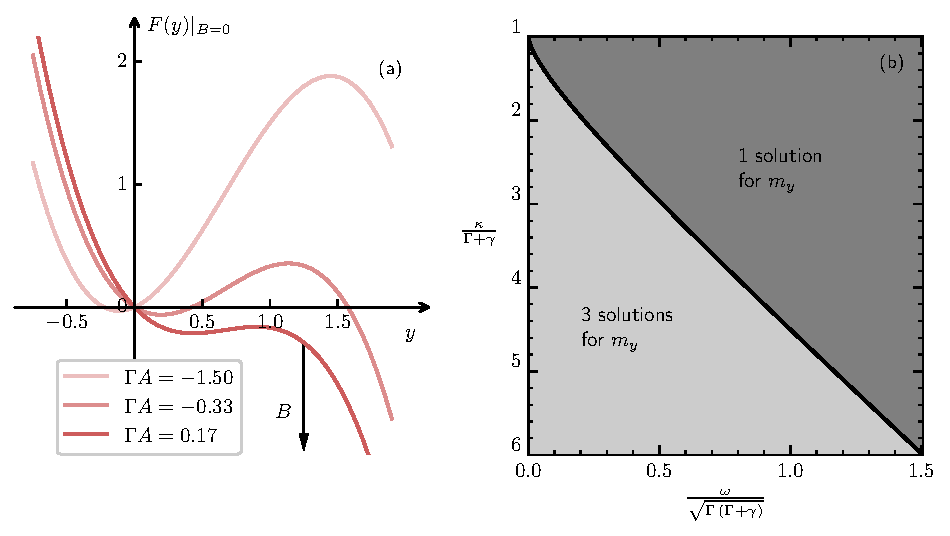
\includegraphics{pictures/polynomial_scheme_phase.pdf}
    \label{fig:numb_fixp}
\end{figure}
For sufficiently large values of $B$, the function is shifted downwards such that only one root survives. Consequently there is a critical constellation of $B$, so that the number of solutions change from one to three. This idea can be made advantage of for calculating the number of fixed points. If the local maximum of $F$ lies below zero, only one root exists.
% \begin{wrapfigure}[19]{l}{0pt}
%     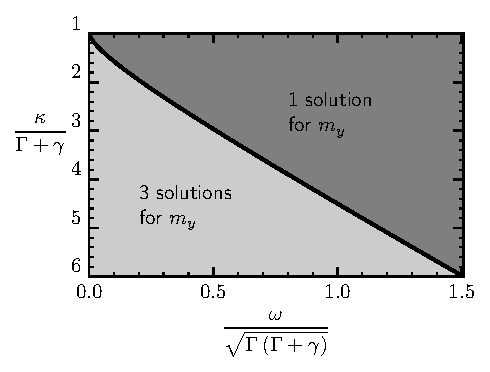
\includegraphics{pictures/numb_fixp2.pdf}
%     \vspace*{-2cm}\caption{The number of fixed points depending on the parameter configuration.}
%     \label{fig:numb_fixp}
% \end{wrapfigure}
With the rescaling $\Omega=\tw/\sqrt{2\,\Gamma\,(\Gamma+\gamma)}$ and $K=\tk/(\sqrt{2}\,(\Gamma+\gamma))$ one gets
\begin{gather*}
    B=\frac{K}{2\,\Omega^2}\\\text{and}\quad
% \end{align*}
% and
% \begin{align*}
    y_\text{max}=\frac{1}{3}\,\left( 2+ \sqrt{1-\frac{3}{2}\,(1-K)\,\frac{1}{\Omega^2}}  \right)
\end{gather*}
and thus the problem only depends on two parameters. Now the border between the configurations with different numbers of fixed points can be determined, by numerically meeting the above mentioned condition of a local maximum with $F(y_{12})=0$. To be explicit this is done by calculating the root of $F(y_{12})$ with respect to $K$ for various values of $\Omega$. The result is shown in \figref{fig:numb_fixp}\\\\As known from previous considerations if $y_\text{max}<1$, i.e. $A>0$ which corresponds to $K>1$, the maximum of $F$ is negative even for $B=0$, resulting in only one solution. Another thing can be noted at this point. As $F(0)=-B$ and $B\neq0$ for $\kappa\neq0$, one solution $m_y$ has always to be negative for $\kappa\neq0$.\\\\

As stable fixed points are possible long-time states of the system, it would be possibly problematic, if they lied outside the physically allowed space, meaning $|m|\leq1/2$. Reassuringly this is never the case as I show in \appref{appendix:mod_of_fixp}. Numerical calculations deliver the same result. I want to mention at this point that in all diagrams that are shown in this thesis $\Gamma=1$ is chosen. All coupling strengths, i.e. energies, are measured in the units of $\Gamma=1$. %
% \begin{wrapfigure}[22]{l}{0pt}
%     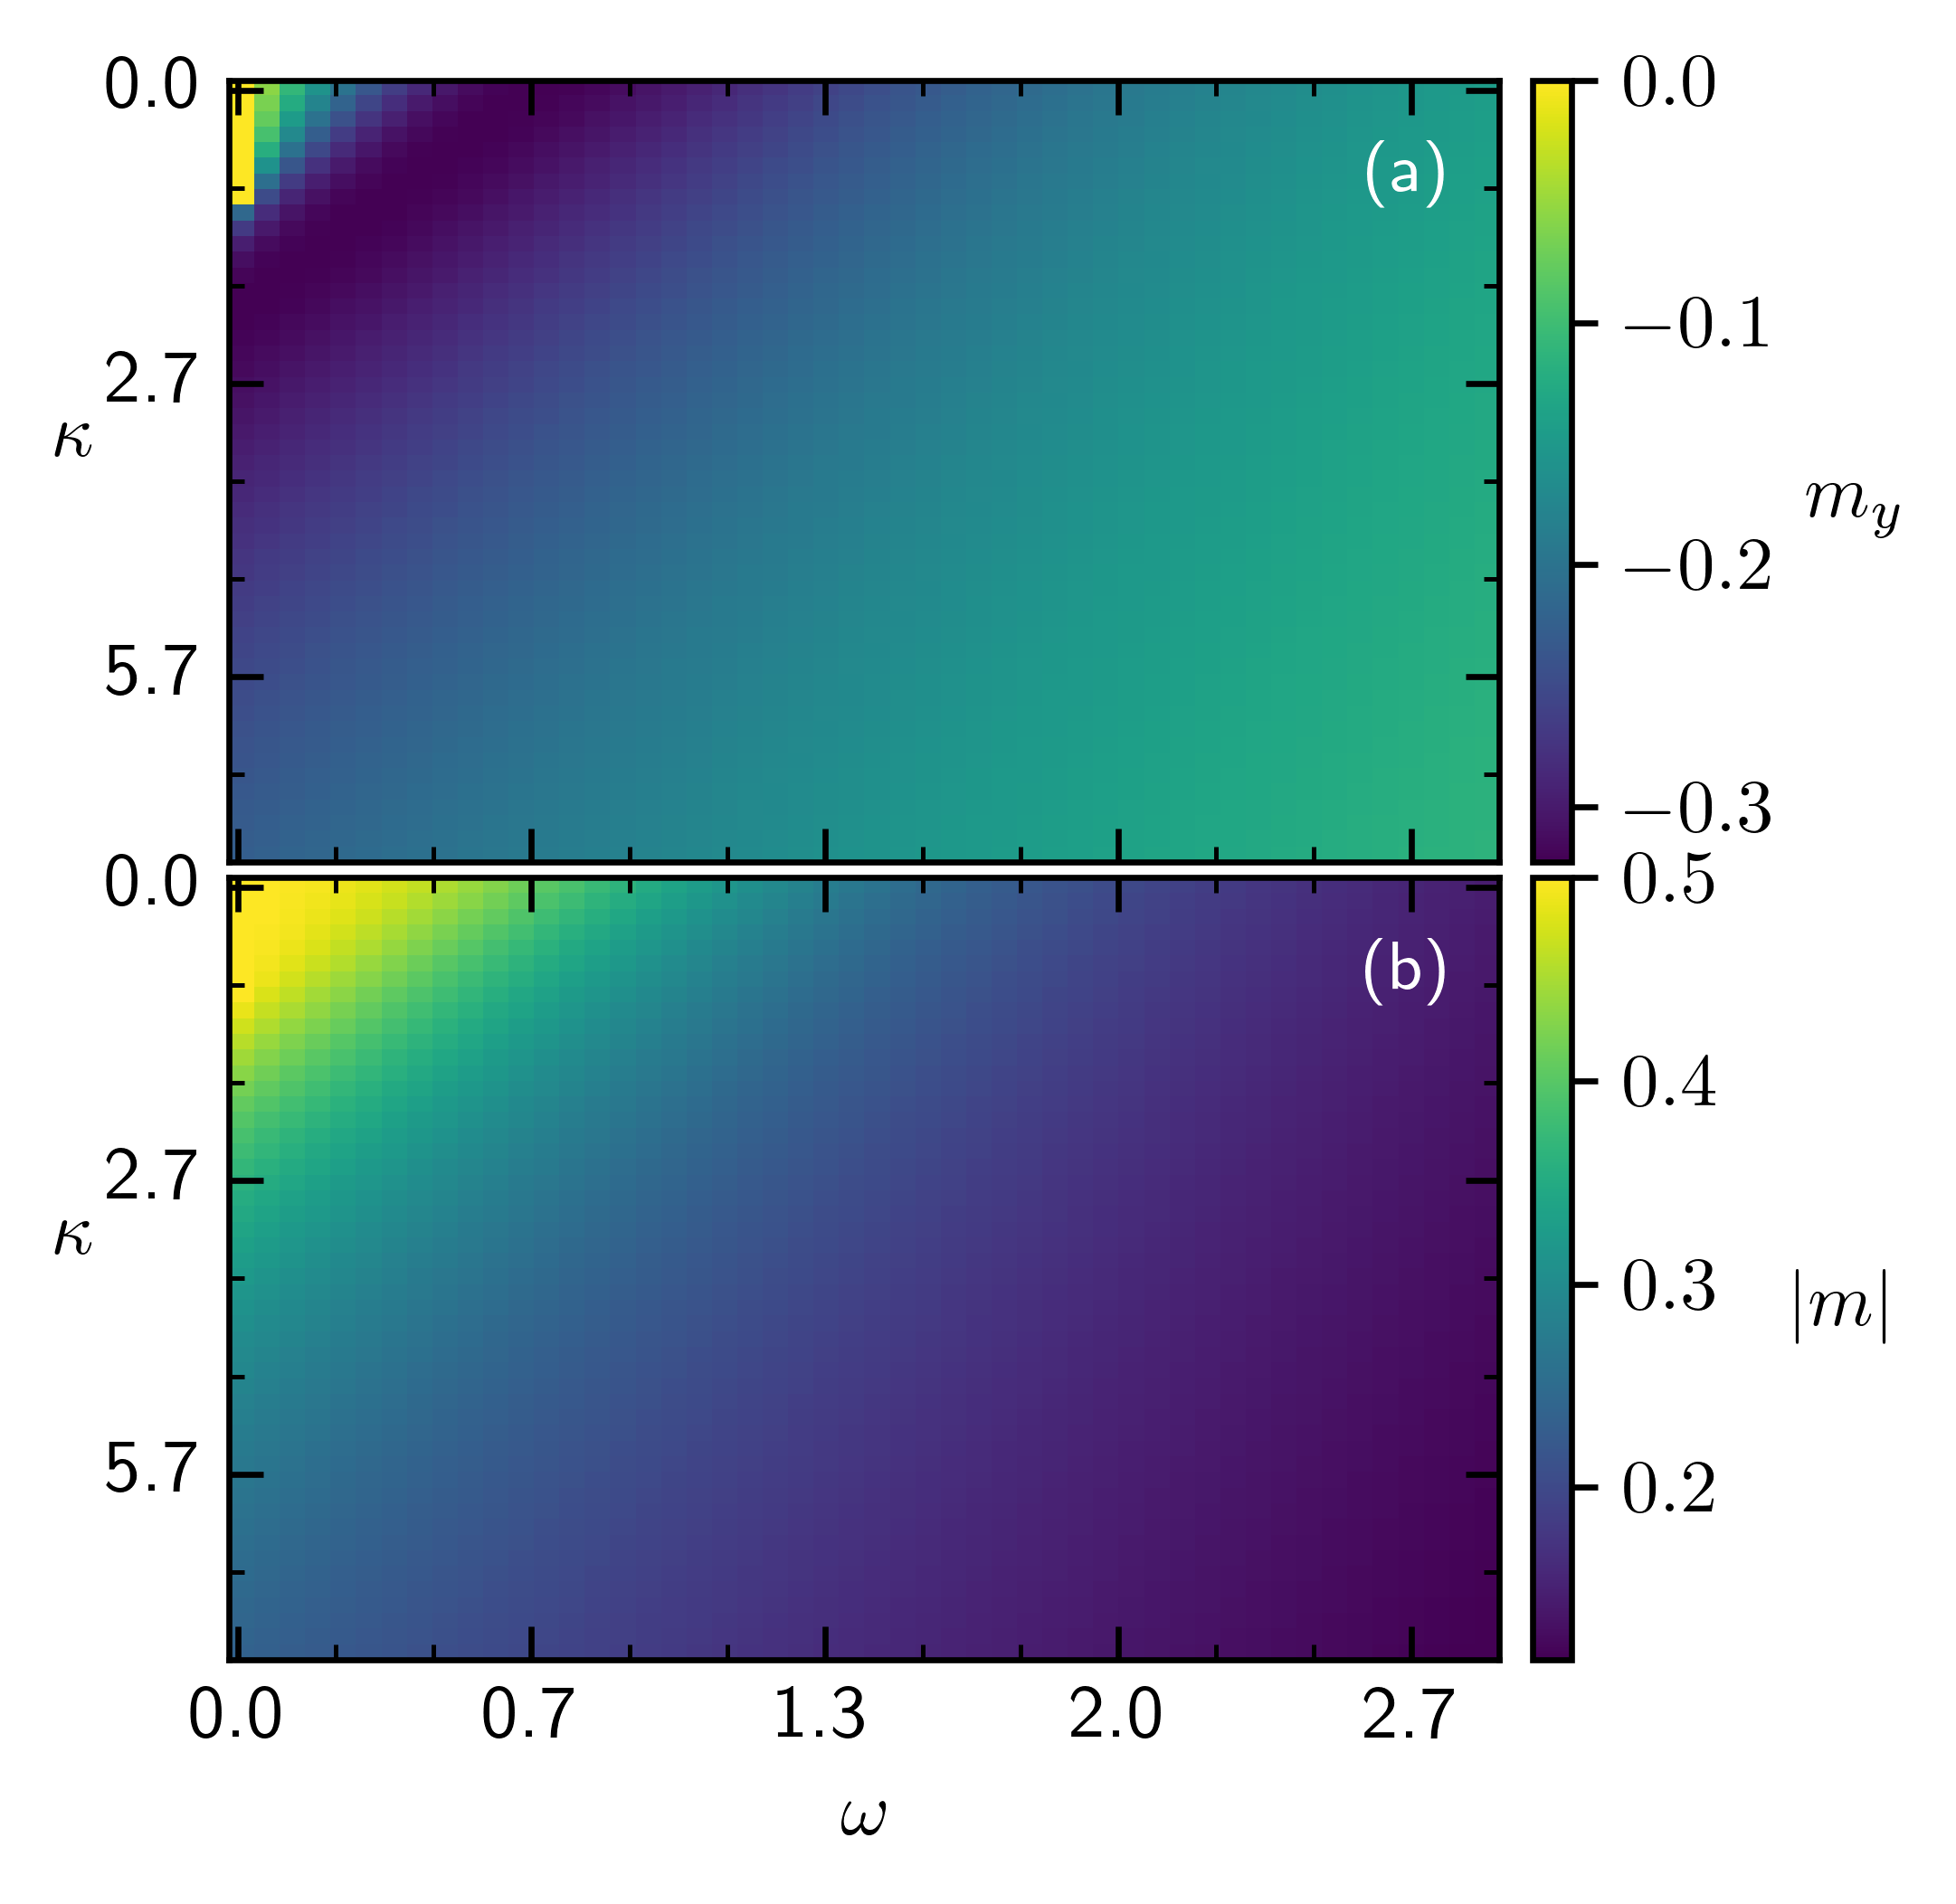
\includegraphics{pictures/fixp_bound_heatmap_s.png}
%     \vspace*{-2cm}\caption{Heatmap for the possible fixed point values for the small $m_y$-solution. (a) depicts $m_y$, whereas (b) depicts $|m|$-values.}
%     
% \end{wrapfigure}
\begin{figure}[H]
    % \floatbox[{\capbeside%\captionsetup[capbesidefigure]%{labelsep=newline}%
    % \thisfloatsetup{capbesideposition={right,center},capbesidewidth=none}}]{figure}[\FBwidth]
    \caption{Heatmap for the possible fixed point values for the small $m_y$-solution. (a) depicts $m_y$, whereas (b) depicts $|m|$-values.}
    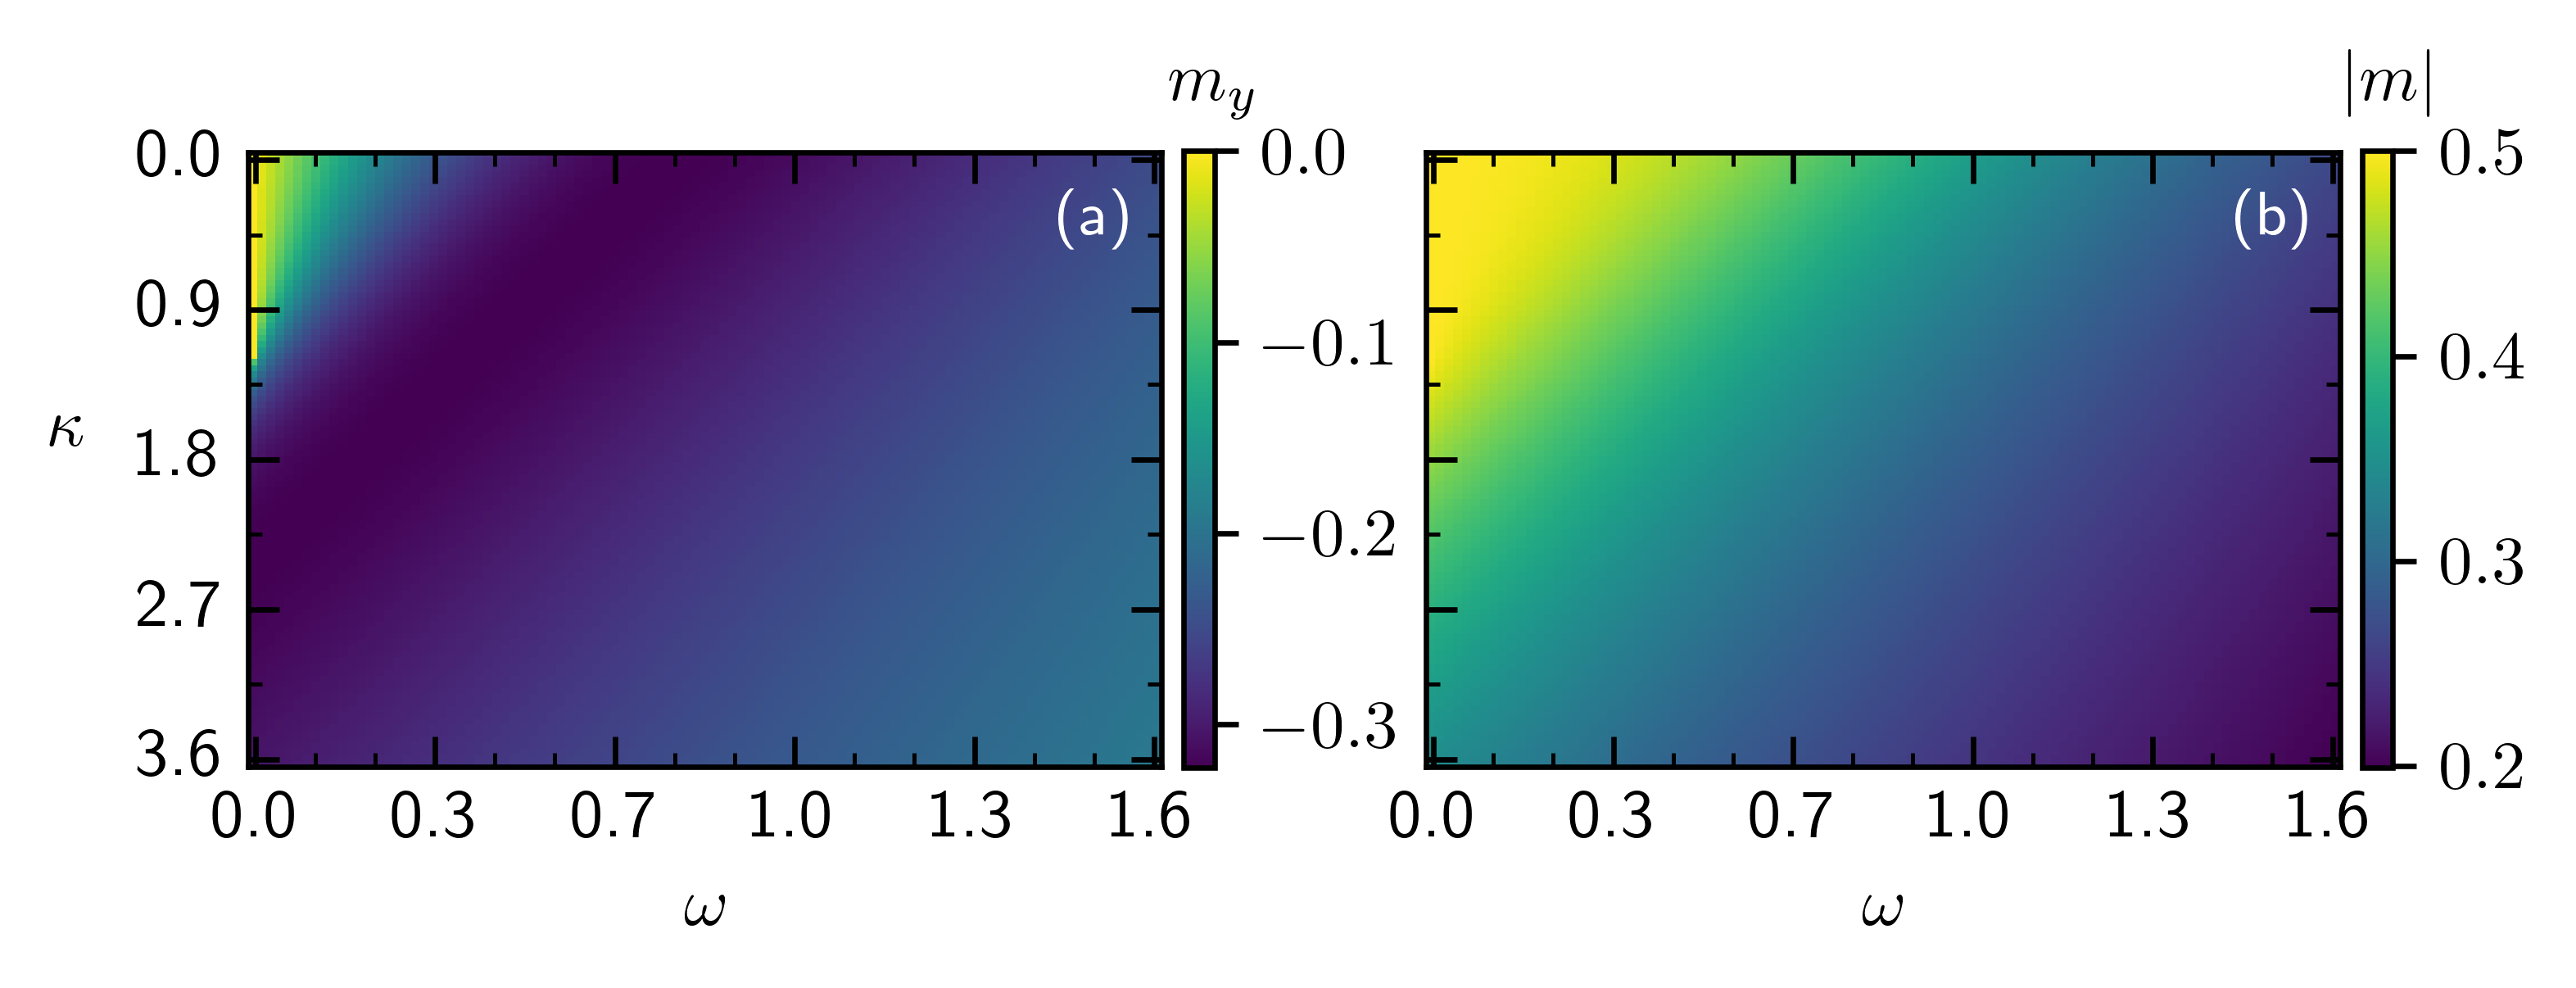
\includegraphics{pictures/fixp_bound_heatmap_s_horiz.png}
    \label{fig:fixp_small_bound_hm}
    %{\label{fig:num_of_fixp_criterium_BF}}
\end{figure}
\begin{figure}[H]
    \vspace*{-0.8cm}
    \hspace*{-1cm}
    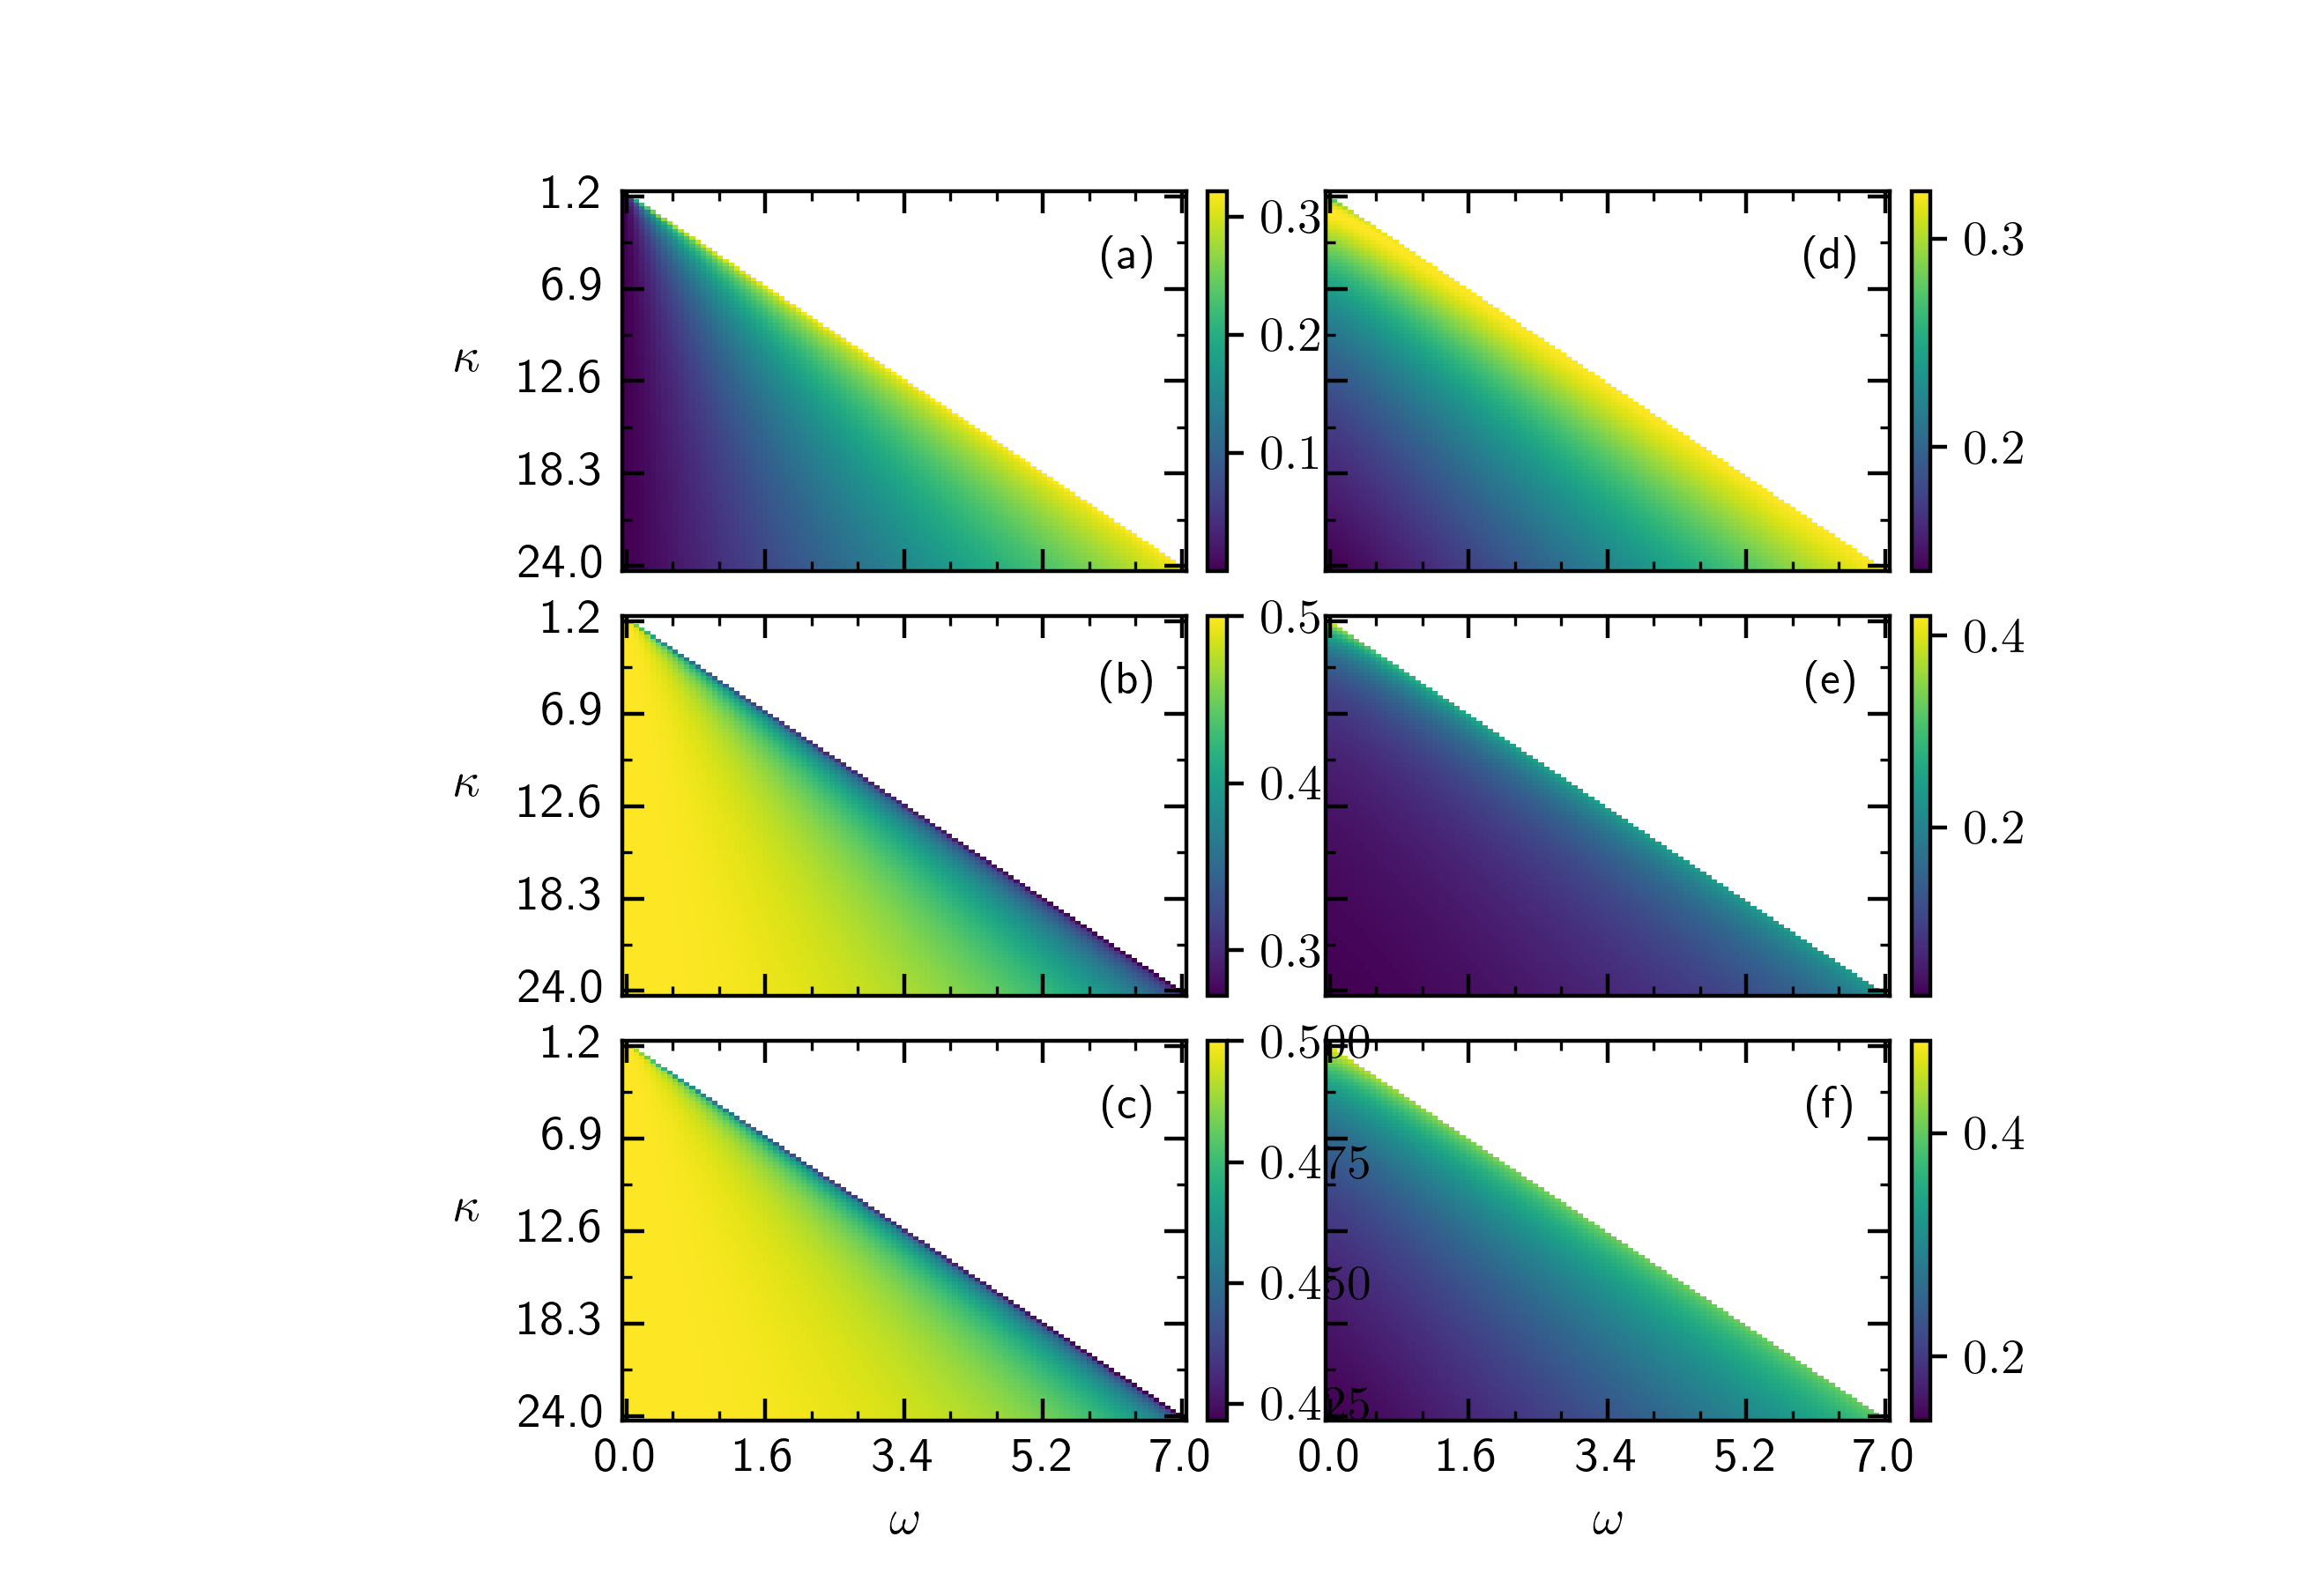
\includegraphics{pictures/fixp_bound_heatmap_ml2.png}
    \caption{heatmap of the range of the fixed point for a certain parameter range of $\omega$ and $\kappa$. $\Gamma=1$, $\gamma=0.2$ are fixed. Presented are properties of the middle $m_y$-solutions in diagrams (a-c) and for the larger $m_y$-solution in (d-f).}
    \label{fig:fixp_midlarge_bound_hm}
\end{figure}
For \figref{fig:fixp_small_bound_hm} and \figref{fig:fixp_midlarge_bound_hm} I calculated components of the collective spin as well as its modular value for different parameter configurations.
The column-like area of $m_y=0$ for small $\kappa$ and $\omega$ in \figref{fig:fixp_small_bound_hm}(a) stems from the fact that for $\omega=0$ and $A>0$ (i.e. $\kappa<\Gamma+\gamma$) $m_y=0$ is the constant solution to the stationary problem. For $A<0$ and $\omega=0$ the $y$-solution grows like $m_y\propto\sqrt{\kappa}$, whereas, for $A>0$ and constant, $m_y$ grows linearly with $\omega$ ($m_y\propto\omega$). Thus the somehow attention grabbing area in the top left corner of the $m_y$ plot can be explained by a constant part of the column at $\omega=0$ together with different grow regimes.
The fixed points are constraint to the physically allowed space, where $|m|\leq1/2$. In some cases the boundary is reached. Especially for the middle $m_y$ fixed point (\figref{fig:fixp_midlarge_bound_hm}(a-c)) $|m|$ is big for a wide range of parameters. Keep in mind that, as $m_z(m_y\rightarrow0)\rightarrow1/2$, the total collective spin reaches it's boundaries for small absolute values of $m_y$.\\\\
Summing up the findings of this paragraph, there are 2 different regions in parameter space. One area, where there exist 3 fixed points, is separated by a nearly linear border from a region of only one stationary solution.


\subsection{Stability analysis}
In order for stationary solutions to play a role in the long-time behavior of the system they need to be stable. This means there has to be at least a small area around the fixed point, so that the system, when starting from a point in this area, ends up in the fixed point for long times. If one makes the region of consideration around the fixed point small enough, the dynamics is governed by the linearization of the equations of motion with respect to $m$. In general one can consider the equation of motion for a function $\mathbf{x}=(x_1,x_2,x_3)^t$ that reads
\begin{align*}
    \dt \mathbf{x}=\mathbf{f}(\mathbf{x})=(f_1(\mathbf{x}),f_2(\mathbf{x}),f_3(\mathbf{x}))^t
\end{align*}
with any differentiable function $\mathbf{f}$. Up to first order in the difference between a point $\mathbf{x}$ and a stationary point of the equation of motion $\mathbf{x}^*$, the dynamics read 
\begin{align*}
    \dt \delta\mathbf{x} \vcentcolon&= \dt\,(\mathbf{x}-\mathbf{x}^*)=D\mathbf{f}|_{\mathbf{x}^*}\,\delta\mathbf{x}\\
    &=\vcentcolon\mathcal{C}\,\delta\mathbf{x}\quad,
\end{align*}
where $D\mathbf{f}|_{\mathbf{x}^*}$ is the Jacobian of $\mathbf{f}$. The emerged linear differential equation is solved by a simple matrix exponential
\begin{align*}
    \delta\mathbf{x}(t)=\delta\mathbf{x}(t=0)\,\exp(\mathcal{C}t)
\end{align*}
For a diagonalizable matrix $\mathcal{C}$, $\delta\mathbf{x}$ can be represented in an eigenbasis of $\mathcal{C}$. The component related to a member of the eigenbasis grows or decays exponentially with the according eigenvalue as rate. For a matrix with all negative eigenvalues a small deviation from the stationary point returns back to it, making this fixed point stable. \\If at least one eigenvalue is positive, the region around the stationary point contains an at least one dimensional subspace, for which points lying on this subspace depart from the fixed point with growing time. \\In this scenario, for an implementation of our model to a real physical system, the presence of unavoidable fluctuations would push the collective spin slightly away from the stable subspace, from where it would exponentially depart from the fixed point\cite{pikovskij_synchronization_2007}. Hence fixed points that are not fully stable will not behave as attractors for the collective spin, even in their vicinity. For the case of an eigenvalue getting zero, one has to turn to the next order for an evaluation of the stability.\\\\
% \begin{figure}[H]
%     \hspace*{-1cm}
%     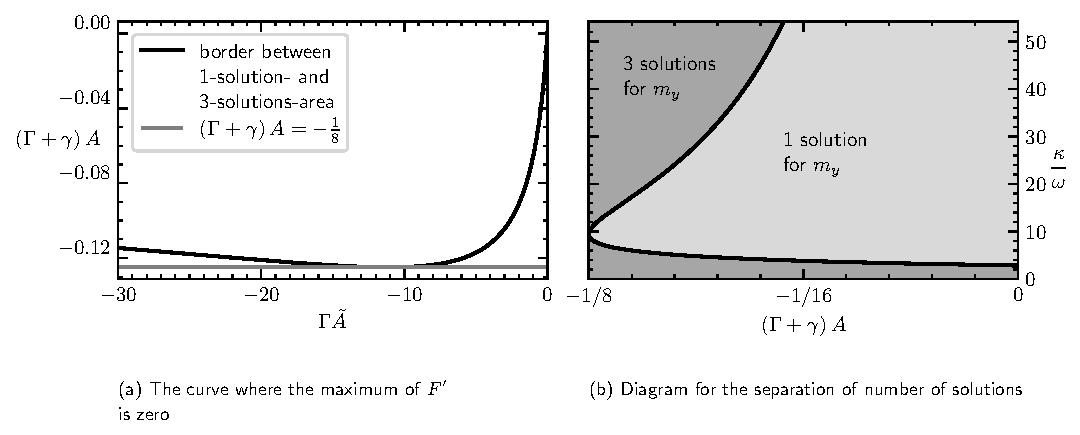
\includegraphics{pictures/phaseplot_A_kw.pdf}
%     \caption{The parameter configurations, where there are 1 ore 3 fixed points can be separated.}
%     \label{fig:phases_numb_of_fixp}
% \end{figure}
With this information in mind one can now move on to the analysis of the stability of the previously found stationary points, knowing that only points, where the linearization matrix has all negative eigenvalues, qualify as certain attractors. The starting of the examination is the calculation of the linear expansion of the equations of motion.
\begin{align*}
    \dt\left(\begin{array}{c}
         \delta m_x\\
         \delta m_y\\
         \delta m_z
    \end{array}\right)&=\left( \begin{array}{ccc}
        -\Gamma\,A-y^2+\frac{\tilde{\omega}}{\tilde{\kappa}}\,y&  0 & 0\\
        0 & -\Gamma\,A-y^2+\frac{\tilde{\omega}}{\tilde{\kappa}}\,y & \sqrt{2}\,\frac{\Gamma}{\tilde{\kappa}^2}\,(\tilde{\kappa}\,y-\tilde{\omega})\\
        0 &  -\sqrt{2}\,\frac{\Gamma}{\tilde{\kappa}^2}\,(2\tilde{\kappa}\,y-\tilde{\omega}) & -2\,\frac{\Gamma^2}{\tilde{\kappa}^2}
    \end{array} \right)\,\left(\begin{array}{c}
         \delta m_x\\
         \delta m_y\\
         \delta m_z
    \end{array}\right)
\end{align*}
For the analysis of the sign of the eigenvalues one is free to multiply the matrix with a positive number, i.e $\tilde{\kappa}^2/\tilde{\omega}^2$, what yields the matrix
\begin{align*}
    \mathcal{C}=\left( \begin{array}{ccc}
        -\Gamma A-{y}^2+{y}&  0 & 0\\
        0 & -\Gamma A-{y}^2+{y}& \sqrt{2}\,\Gamma/\tilde{\kappa}\,({y}-\frac{\tilde{\kappa}}{\tilde{\omega}})\\
        0 &  -\sqrt{2}\,\Gamma/\tilde{\kappa}\,(2\,{y}-\frac{\tilde{\kappa}}{\tilde{\omega}}) & -2\,\frac{\Gamma^2}{\tilde{\omega}^2}
    \end{array} \right)
\end{align*}
The first eigenvalue is already accessible due to the block form of the matrix. In order to determine the sign of the first eigenvalue in general, it is convenient to define an even more general parameter
% \begin{wrapfigure}[16]{l}{0pt}
\begin{figure}[H]
    \centering
    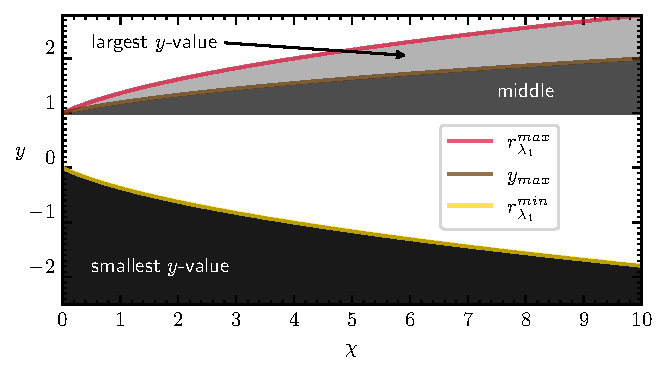
\includegraphics{pictures/sign_of_ev1_streched.pdf}
    % \vspace*{-2cm}
    \caption{The smaller ($r_{\lambda_1}^{min}$) and larger ($r_{\lambda_1}^{max}$) roots of $\lambda_1$ with marked areas for the value for ${y}=k/w\cdot m_y$. ${y}_{max}$ is the ${y}$-position of $F$.}
    \label{fig:sign_lam1}
\end{figure}
% \end{wrapfigure}
\begin{gather*}
    \chi\vcentcolon=\frac{K-1}{\Omega^2}\\
    \Rightarrow\quad\Gamma A=-\half\,\chi,\quad
    B=\half\,\chi+\frac{1}{2\,\Omega^2}%\frac{K}{2\,\Omega^2}&=\frac{K-1}{2\,\Omega^2}+\frac{1}{2\,\Omega^2}=\half\,\chi+\frac{1}{2\,\Omega^2}
\end{gather*}
The first eigenvalue is in the form of a second order polynomial in $y$ and has therefore in general 2 roots. Between the two roots the eigenvalue is positive marking the fixed point as unstable, where as outside the interval between the roots the eigenvalue is negative, maintaining the possibility of a stable fixed point. When the parameter $\chi$ gets negative \figref{fig:sign_lam1} shows, that the roots of $\lambda_1$ lie both in the region $y>0$. From the previous consideration it is known, that only one fixed point exists for $\chi<0$, i.e $K<1$, and it is negative. Thus for $\chi<0$ the first eigenvalue is always negative.\\\\
Turning to the case $K>1$. Here 3 fixed points are possible. Picturing a possible course of the polynomial of third degree, whose solutions resemble the $y$-values of the fixed points one can make a few statements on the position of those fixed points. The smallest solution, which is always negative, has its maximal value for the shift $B$ being minimal. For a given parameter configuration, it always holds $B<\chi/2$. So the values of the smallest solution, if $B$ is replaced by $\chi$ are always larger as the true solution. In fact $B\rightarrow\chi$ when $\Omega\rightarrow\infty$ and also $K$ diverges in a way that keeps $\chi$ constant.
\begin{align*}
    \tilde{F}({y})=-\half\,\chi-(1-\half\,\chi)\,{y}    - {y}^3+2\,{y}^2
\end{align*}
% For a given value of $\chi$ the parameter $\Omega$ can be chosen freely, because through an appropriate choice of $K$ the value of $\chi$ can be fixed. So for every possible value of $\chi>0$ the supreme value of $B$ is just $\chi/2$, as $\Omega\rightarrow\infty$.
% The first, smallest fixed point has again because of the positive sign of $B$ always a negative $y$-component. It has it's greatest value for minimal $B$. Negative values of $\chi$ lead to positive roots of $\lambda_1$, which induces that $\lambda_1$ itself is negative. \\\\
It turns out that the roots of $\lambda_1$ are always a root of $\tilde{F}$. Consequently the true $y$-value of the fixed point, with smallest $y$, is always smaller than the root of $\lambda_1$ and therefore this fixed point has a negative first eigenvalue.\\\\
So I will move on to the next fixed point, the one in the middle. It also takes its smallest value for minimal $B$, allowing one to look at the function $\tilde{F}$ again. In this constellation the middle root is always at ${y}=1$. The maximal possible $y$-value (actually supremum) for the middle fixed point is at the maximum point of $F$ which is also the minimal possible value of the largest root. The maximum $y$-value of the largest fixed point, is again for minimal $B$ and thus the larger root of $\lambda_1$ is a supremum of this fixed point.\\\\
In summary one can state that the first eigenvalue of the smallest-$y$ solution is always negative, whereas the eigenvalue of the other possible fixed points is always positive, identifying them as unstable. \\\\As unstable fixed points are from a physical perspective not as significant, I will focus in the following part of the discussion mainly on the fixed point with smallest $y$-solution. The stability of this stationary solution is yet to be determined by evaluating the remaining eigenvalues.
% $K$ and $\Omega$ can always be adopted in a way, so that $\chi$ and $1/\Omega^2$ can take every arbitrarily large number.
% \begin{gather*}
%     \frac{K-1}{\Omega^2}=\chi, \quad \frac{1}{\Omega^2}=M\\
%     \Rightarrow K=1+\frac{\chi}{M}\quad\text{and}\quad\Omega = \frac{1}{\sqrt{M}}
% \end{gather*}
% Thus the true $B$ can be made arbitrarily big while $\chi$ stays as it is, allowing in turn, that the fixed point, with the largest $y$-value, gets arbitrarily large.
% So we can already provide a diagramm for the possible sign-values of $\lambda_1$ in \autoref{fig:sign_lam1}.\\\\
This analysis will be performed numerically. Thus there is less need for rescaling quantities, instead it is often more convenient to stick to the original form, in order to avoid unnecessary pols. In this form $m_y$ is determined by the equation
\begin{align*}
    0=&-\half\,\Gamma\omega-(\half\,\Gamma\,(\Gamma+\gamma-\kappa)+\omega^2)\,m_y\\&-\kappa^2\,m_y^3+2\,\kappa\omega\,m_y^2
\end{align*}
and the linearization of the equations of motion result in the following matrix.
\begin{align*}
    \Gamma\,\mathcal{C}=&\left( \begin{array}{c c c}
        -\half\,\Gamma\,(\Gamma+\gamma-\kappa)-\kappa^2\,m_y^2
        +\omega\kappa\,m_y&0&0\\
        0&-\half\,\Gamma\,(\Gamma+\gamma-\kappa)-\kappa^2\,m_y^2
        +\omega\kappa\,m_y&\Gamma\,(\kappa\,m_y-\omega)\\
        0&-\Gamma\,(2\kappa\,m_y-\omega)&-\Gamma^2
    \end{array}  \right)
\end{align*}

% \begin{wrapfigure}[29]{l}{0pt}
%     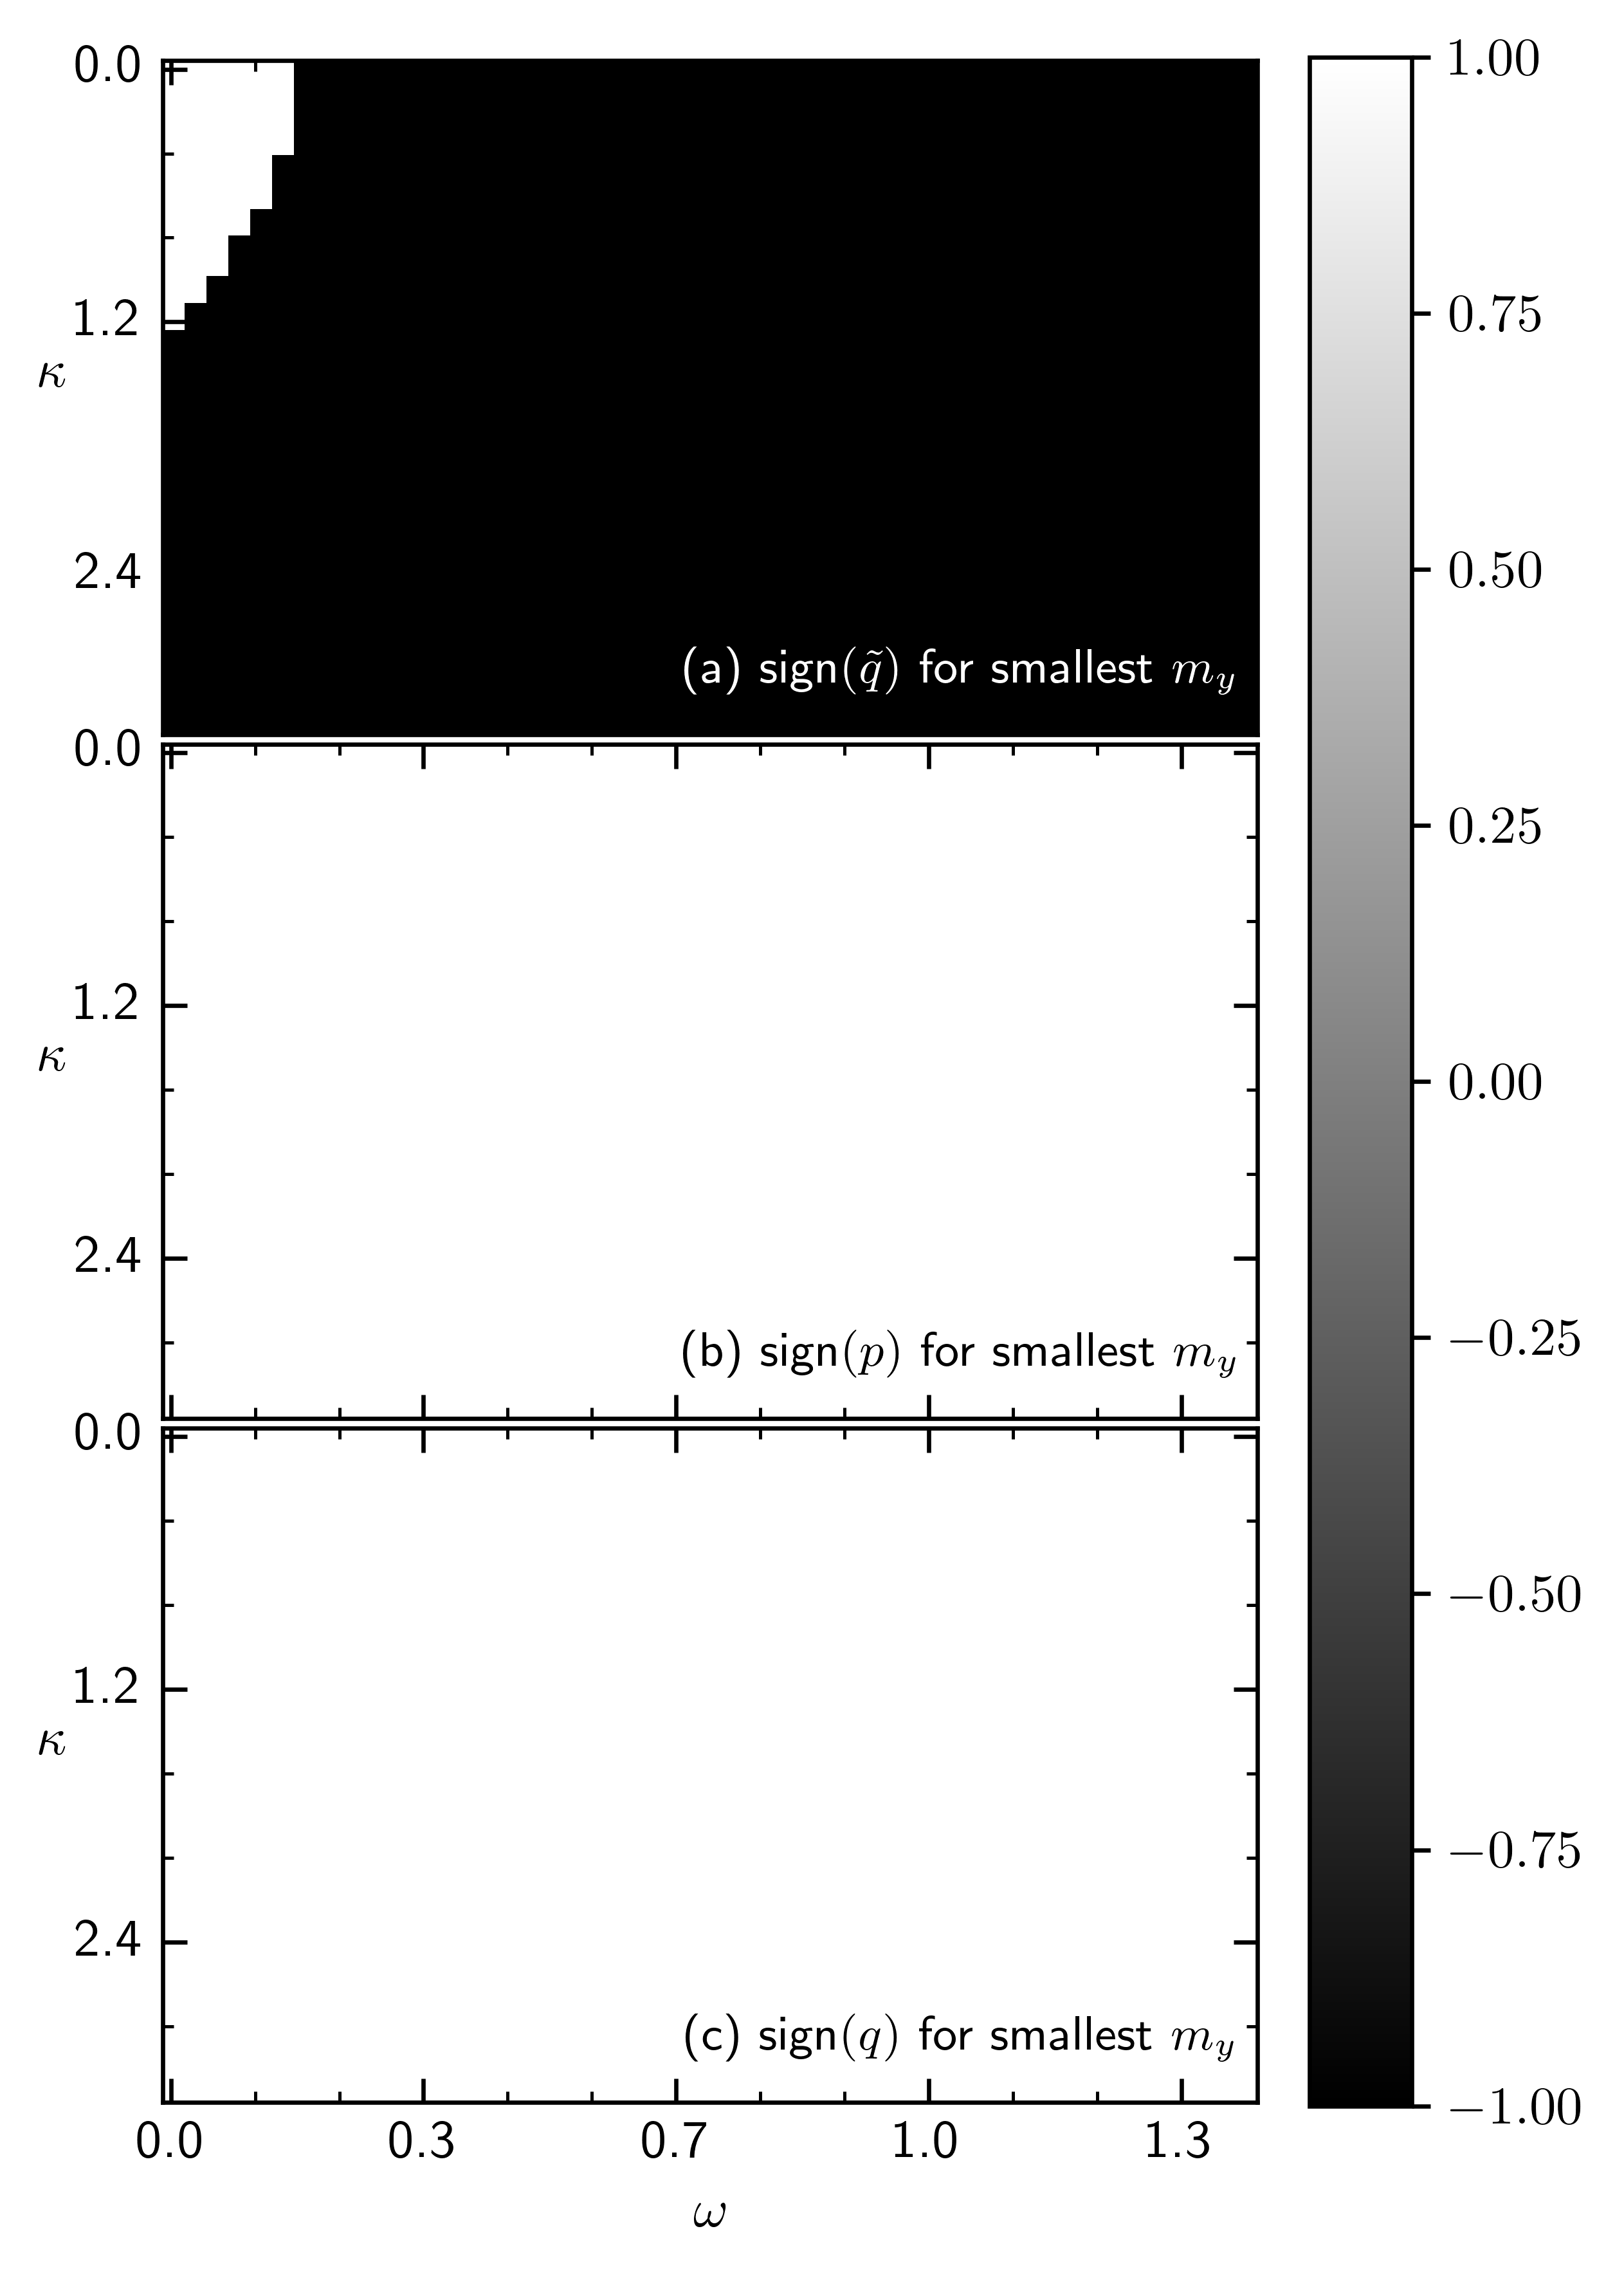
\includegraphics{pictures/lam2_anal_s.png}
%     \vspace*{-2cm}\caption{Heatmap for the possible fixed point values for the small $m_y$-solution. (a) depicts $m_y$, whereas (b) depicts $|m|$-values.}
%     \label{fig:sign_lam23_s}
% \end{wrapfigure}


The remaining two eigenvalues of the fixed points are the eigenvalue of the lower $2\times2$-block of the linearization matrix and are determined by the $\lambda$-roots of the expression
\begin{align*}
    0&=\lambda^2+\left( \Gamma^2 +\half\,\Gamma\,(\Gamma+\gamma-\kappa)+\kappa^2\,m_y^2
    -\omega\kappa\,m_y\right)\,\lambda\\
    &+\Gamma^2\,(\half\,\Gamma\,(\Gamma+\gamma-\kappa)+\kappa^2\,m_y^2-\omega\kappa\,m_y)\\
    &+\Gamma^2\,(\kappa\,m_y-\omega)\,(2\,\kappa\,m_y-\omega)\\
    &=\vcentcolon t^2+p\,t+q\\
    \Rightarrow\quad\lambda_{23}&=\half\,(-p\pm\sqrt{p^2-4q})\quad.
\end{align*}
% or
% \begin{align*}
%     0=&\,t^2+\left( 2\,\frac{\Gamma^2}{\tilde{\omega}^2}+\Gamma\tilde{A}+y^2-y \right)\,t\\
%     &+2\,\frac{\Gamma^2}{\tilde{\omega}^2}\,\left( \Gamma\tilde{A}+y^2-y \right)\\
%     &+2\,\frac{\Gamma^2}{\tilde{\kappa}^2}\,(2\,y-\frac{\tilde{\kappa}}{\tilde{\omega}})\,(y-\frac{\tilde{\kappa}}{\tilde{\omega}})\\
%     &=\vcentcolon t^2+p\,t+q\\
%     \Rightarrow\quad\lambda_{23}=&\half\,(-p\pm\sqrt{p^2-4q})\quad.
% \end{align*}
When $q$ becomes negative, the square root gets larger in absolute value than $p$ and thus one eigenvalue is positive, resulting in an unstable fixed point. On the other hand, when $p$ and $q$ are both positive, both eigenvalues $\lambda_{23}$ have negative real part.

\begin{figure}[H]
    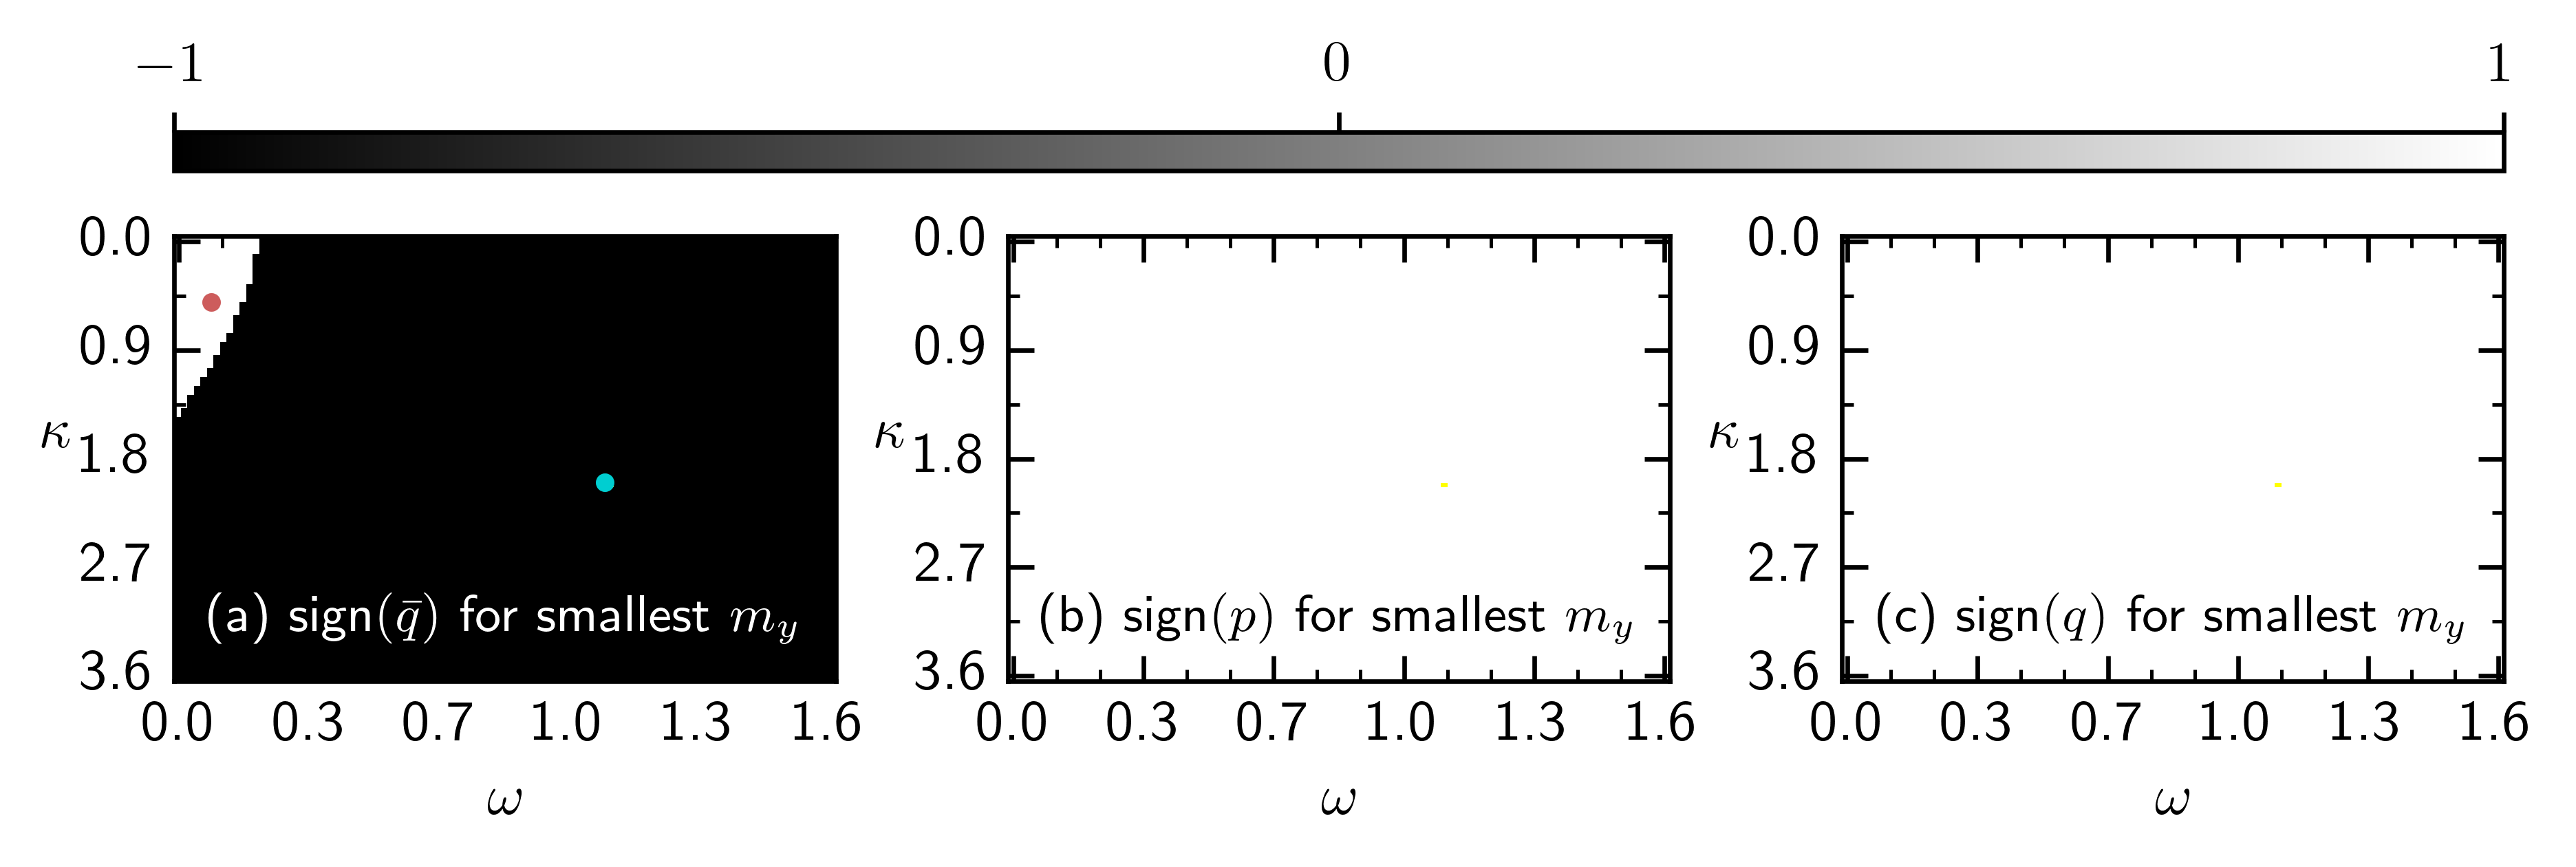
\includegraphics{pictures/lam2_anal_s2.png}
    \caption{Sign analysis of eigenvalue 2 and 3 for the smallest $y$-valued stationary point. In (a) the sign of the interior of the square root, involved in the formula for these eigenvalues, is shown and hence complex eigenvalues are indicated. For the red and blue dots exemplary trajectories are plotted below, confirming the presence or absence of oscillatory behavior. (b) and (c) show that the sign of the quantities $p$ and $q$.}% are both always positive, and thus the whole eigenvalue has negative real part.}
    \label{fig:sign_lam23_s}
\end{figure}%
As can be observed from \figref{fig:sign_lam23_s} (b)-(c) $p$ and $q$ are always positive for the fixed point with smallest $y$-value and hence this stationary point is stable for all considered parameter configurations.\\
From the information, whether the eigenvalues are real or complex, a hint about the type of the dynamics can be derived. In the case of complex eigenvalues, which arise, if the discriminant of the characteristic polynomial $\bar{q}\vcentcolon=p^2-4q$ gets negative,  the matrix exponential has an oscillatory part. This is expected to also show in the full dynamics, if the system is sufficiently close to such a stationary point. To confirm this I took one parameter configuration in each of the two regions, where the eigenvalues become complex versus where they stay real. Their location is shown in \figref{fig:sign_lam23_s} (a). For those parameter configurations I calculated four exemplary trajectories starting at random points in the spin space, which are depicted in \figref{fig:expl_traj_d0}.
% Starting with the analysis of $p$ and going back one last time in the rescaled form with the above defined new parameters, one finds
% \begin{align*}
%     p=&\frac{\Gamma}{\Omega^2\,(\Gamma+\gamma)}-\half\,\chi+3\,y^2-4\,y+1
% \end{align*}
% the roots of this expression, which are maximally apart from each other, are found, when $\Omega\rightarrow\infty$ in the same spirit as above. This yields as roots of $p$
% \begin{align*}
%     r_p=&\frac{1}{3}\,\left( 2\pm\sqrt{1+\frac{3}{2}\,\chi-3\,\frac{\Gamma}{\Omega^2\,(\Gamma+\gamma)}} \right)\\
%     r_p^\text{max}=&\frac{1}{3}\,\left( 2+\sqrt{1+\frac{3}{2}\,\chi} \right)\\
%     r_p^\text{min}=&\frac{1}{3}\,\left( 2-\sqrt{1+\frac{3}{2}\,\chi} \right)
% \end{align*}
% One can recognize, that $r_p^\text{max}=\tilde{y}_\text{max}$ and $r_p^\text{min}=\tilde{y}_\text{min}$. Thus we can infer that for the bracketing fixed points $p$ is always positive, whereas for the middle fixed point we can't make this statement. Together with the finding that $q$ is positive this induces that the fixed point with smallest $y$-value is stable.\\\\
% For the unstable fixed points the analysis of the eigenvalues $\lambda_{23}$ is done numerically by the computing the expression
% \begin{align*}
%     \lambda_{23}=&\half\,(-p\pm\sqrt{p^2-4q})\quad.
% \end{align*}
% When $q$ becomes negative, the square roots gets larger in absolute value than $p$ and thus one eigenvalue is positive, resulting in an unstable fixed point. On the other hand, when $p$ and $q$ are both positive, both eigenvalues $\lambda_{23}$ have negative real part. The eigenvalues become complex and allow for oscillatory behavior near the fixed point if the interior of the square root, labeled as  
% \begin{align*}
%     \bar{q}\vcentcolon=p^2-4q\quad.
% \end{align*}
% get's negative. To describe the properties of the fixed points we investigate the three values $p$, $q$ and $\bar{q}$. %As already mentioned a negative $\bar{q}$ signals complex eigenvalues. In this case $-p$ is the real part of the eigenvalue. On the other hand when $q$ gets negative the eigenvalues $\lambda_2$ and $\lambda_3$ have different signs, whereas when $q\geq0$ the eigenvalues $\lambda_{23}$ have always the oposite sign of $p$
\begin{figure}[H]
    \centering
    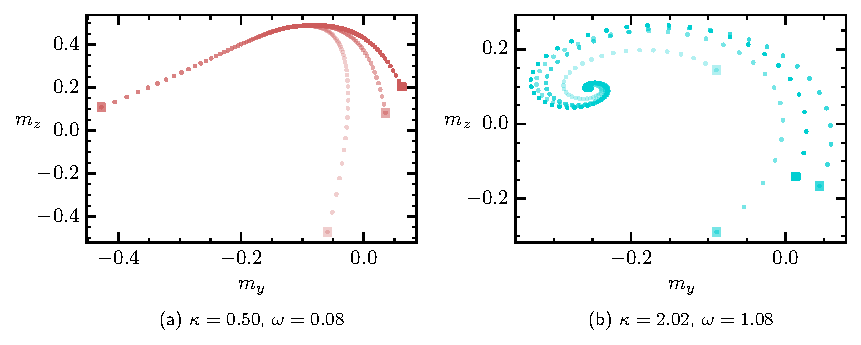
\includegraphics{pictures/example_traj_d0.pdf}
    \caption{For the two different parameter constellations in the area of complex (b) and all real (a) eigenvalues four trajectories are plotted starting at randomly chosen starting points. The starting points are marked by squares. In the two figures the different level of opacity is used to differentiate the trajectories.
    }
    \label{fig:expl_traj_d0}
\end{figure}

The evaluated trajectories show the expected behavior. Whereas for the case of all real eigenvalues the collective spin decays in a straight forward fashion to its stationary point, for complex eigenvalues the origin of oscillatory behavior arises. %Nevertheless for the case of $\delta=0$ these oscillations are damped, bringing the system for long times to a constant stationary point.
\\\\An indication to the speed of this decay is given by the magnitude of the eigenvalues, which are plotted in \figref{fig:eig_value_stab1} and \figref{fig:eig_value_stab2}. The less significant values of the unstable fixed points are shown in \appref{appendix:eig_del0} for completeness.

\begin{figure}[H]
    \centering
    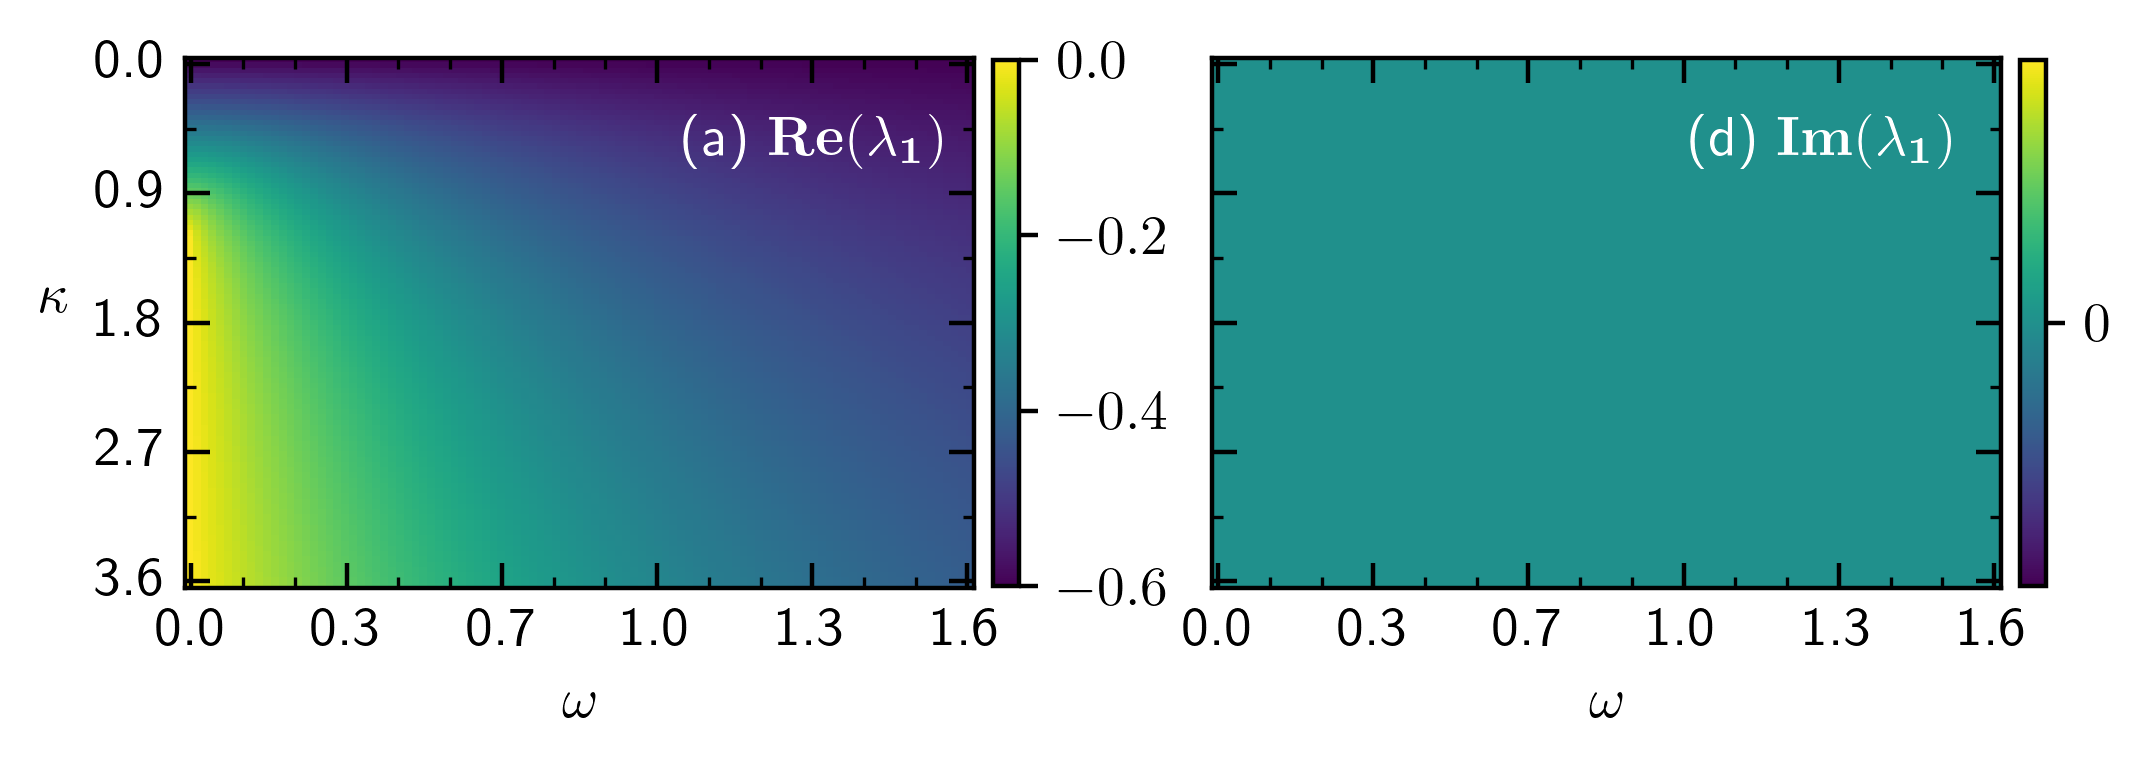
\includegraphics{pictures/lam_anal_s_1.png}
    \caption{In this graph the first eigenvalue of the fixed point with the smallest $y$-value are plotted.}
    \label{fig:eig_value_stab1}
\end{figure}
\begin{figure}[H]
    \centering
    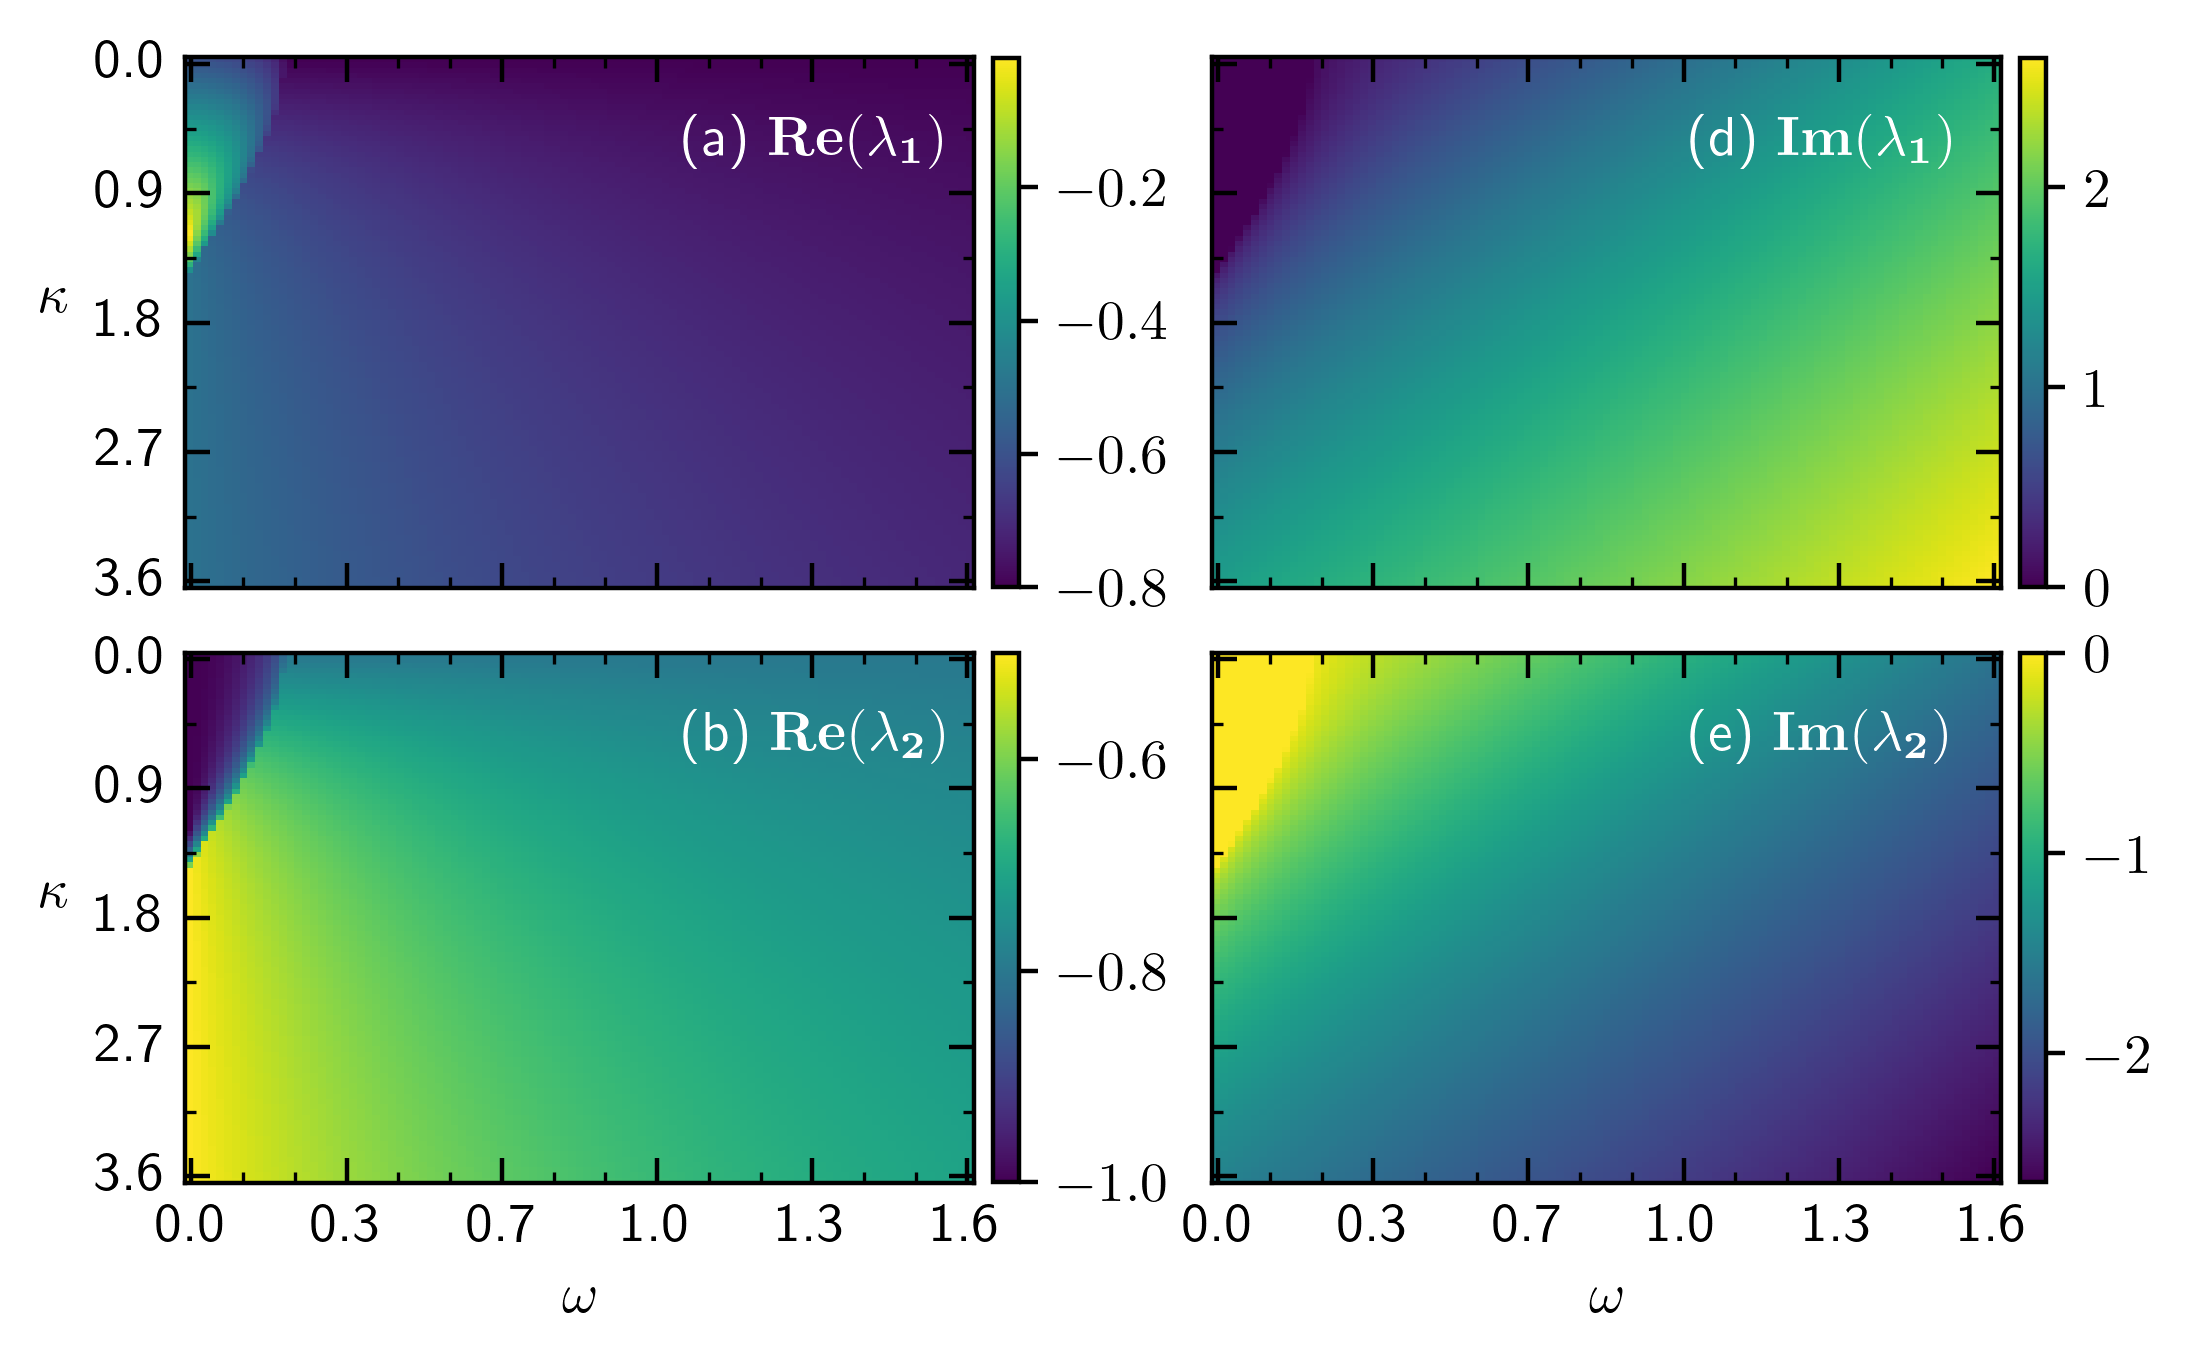
\includegraphics{pictures/lam_anal_s_2.png}
    \caption{In this graph the second and third eigenvalue of the fixed point with the smallest $y$-value are plotted. Notice the region of small $\kappa$ and $\omega$ in the top left corner of the real and imaginary parts of the eigenvalues. Here the real part changes rather quickly, which stems from the square root becoming real (\figref{fig:sign_lam23_s}).
    }
    \label{fig:eig_value_stab2}
\end{figure}

By studying the constraint of zero detuning, I was able to perform a good part of the characterization of that system analytically. This allowed to get an intuition on how changes in the equations of motion due to different parameter values can influence the existence and stability of fixed points. Without detuning I found that the system always decays to a stationary fixed point, indifferently whether there were 3 or 1 stationary solutions to the equation of motion. Nevertheless outsets of oscillatory dynamics have been observed, giving rise to the question, whether the onset of detuning can change the stability of those oscillations. 

% % \clearpage
% \chapter{Dynamics in the thermodynamic limit}
\newpage
\section{Analysis for the detuned driving}\label{sec:detuned_analysis}%[Detuned driving]
After I examined the system in resonance with the driving laser, it is interesting to see if the stability of the system remains when a detuning is introduced. As the presence of a small detuning can not be completely avoided in reality, it is important to examine if the previously found properties withstand the onset of detuning, and are thus actually observable.\\
For the non-resonant driving $m_x=0$ is no stationary solution anymore, on the contrary $m_x$ and $m_y$ are coupled by the detuning in an oscillatory way. One can wonder, if this additional oscillation inducing term can effect the system in a way that the oscillations do not die out. In fact this is true. In this section I will show the rise of time crystal regimes and dedicate the section to two properties of the system, that I find most interesting. On the one hand subregions are found where more than one limit cycle exists for the same parameter configuration and hence multistability arises. Additionally the division of the dynamics into a region of stationary and time crystal solutions will be linked to synchronization behavior. The start of the analysis will again constitute the search for stable fixed points.


\subsection[stability in general]{Stability analysis of the fixed points}\label{sec:stab_3D}
The procedure by which the number of fixed points is determined as well as their stability is the same as previously. Because of the more complex structure of the equations of motion with detuning present the analysis will be performed numerically.\\
In this context the following system of equations is solved for stationary $m_x$- and $m_y$-values
\begin{align*}
    -\Gamma\delta\,m_y-\Gamma\,(\gamma+\Gamma-\kappa)\,m_x-2\,\kappa^2\,m_x\,( m_x^2+ m_y^2)+2\,\kappa\omega\,m_xm_y  &=0\\\\
    \Gamma\delta\,m_x-\omega\Gamma-\Gamma\,(\gamma+\Gamma-\kappa)\,m_y-2\,\omega^2\,m_y&\\
    -2\,\kappa^2\,m_y\,( m_x^2+ m_y^2)+2\,\kappa\omega\,(m_x^2+2\,m_y^2)  &=0\quad.
\end{align*}
% After multiplying the first equation by $m_y$ and the second by $m_x$, the two equations can be subtracted from each other.
% \begin{align*}
%     -\Gamma\delta\,(m_x^2+m_y^2)+\Gamma\omega\,m_x+2\,\omega^2\,m_xm_y-2\,\kappa\omega\,m_x\,(m_x^2+m_y^2)
% \end{align*}
% By solving this quadratic equation for $m_y$ analytically and plugging the result into the second equation, one has two find a root of a one variable function, which is computationally less expensive than determining the roots of the two dimensional problem. For the pursuit of this procedure I divided the x-axis into a grid and searched between the gridpoints for roots in order to find all of the fixed points.\\
% In critical regions, where this procedure did not work well, I created a 2D grid and solved the two dimensional problem.\\\\
As a result of the numerical calculation one finds, that there again exist two regions, one in which there is one fixed point and one in which three fixed points are present. The $\delta=0$ case is expanded continuously.
% \begin{align*}
%     m_{y,12}(m_x)=\frac{1}{\Gamma\delta+2\,\kappa\omega\,m_x}\,\left( \omega^2\,m_x\pm \sqrt{\omega^4\,m_x^2-(\Gamma\delta+2\,\kappa\omega\,m_x)\,[(\Gamma\delta+2\,\kappa\omega\,m_x)\,m_x^2-\Gamma\omega\,m_x]} \right)
% \end{align*}
\begin{figure}[H]
    % \vspace*{-1cm}
    \hspace*{-1.2cm}
    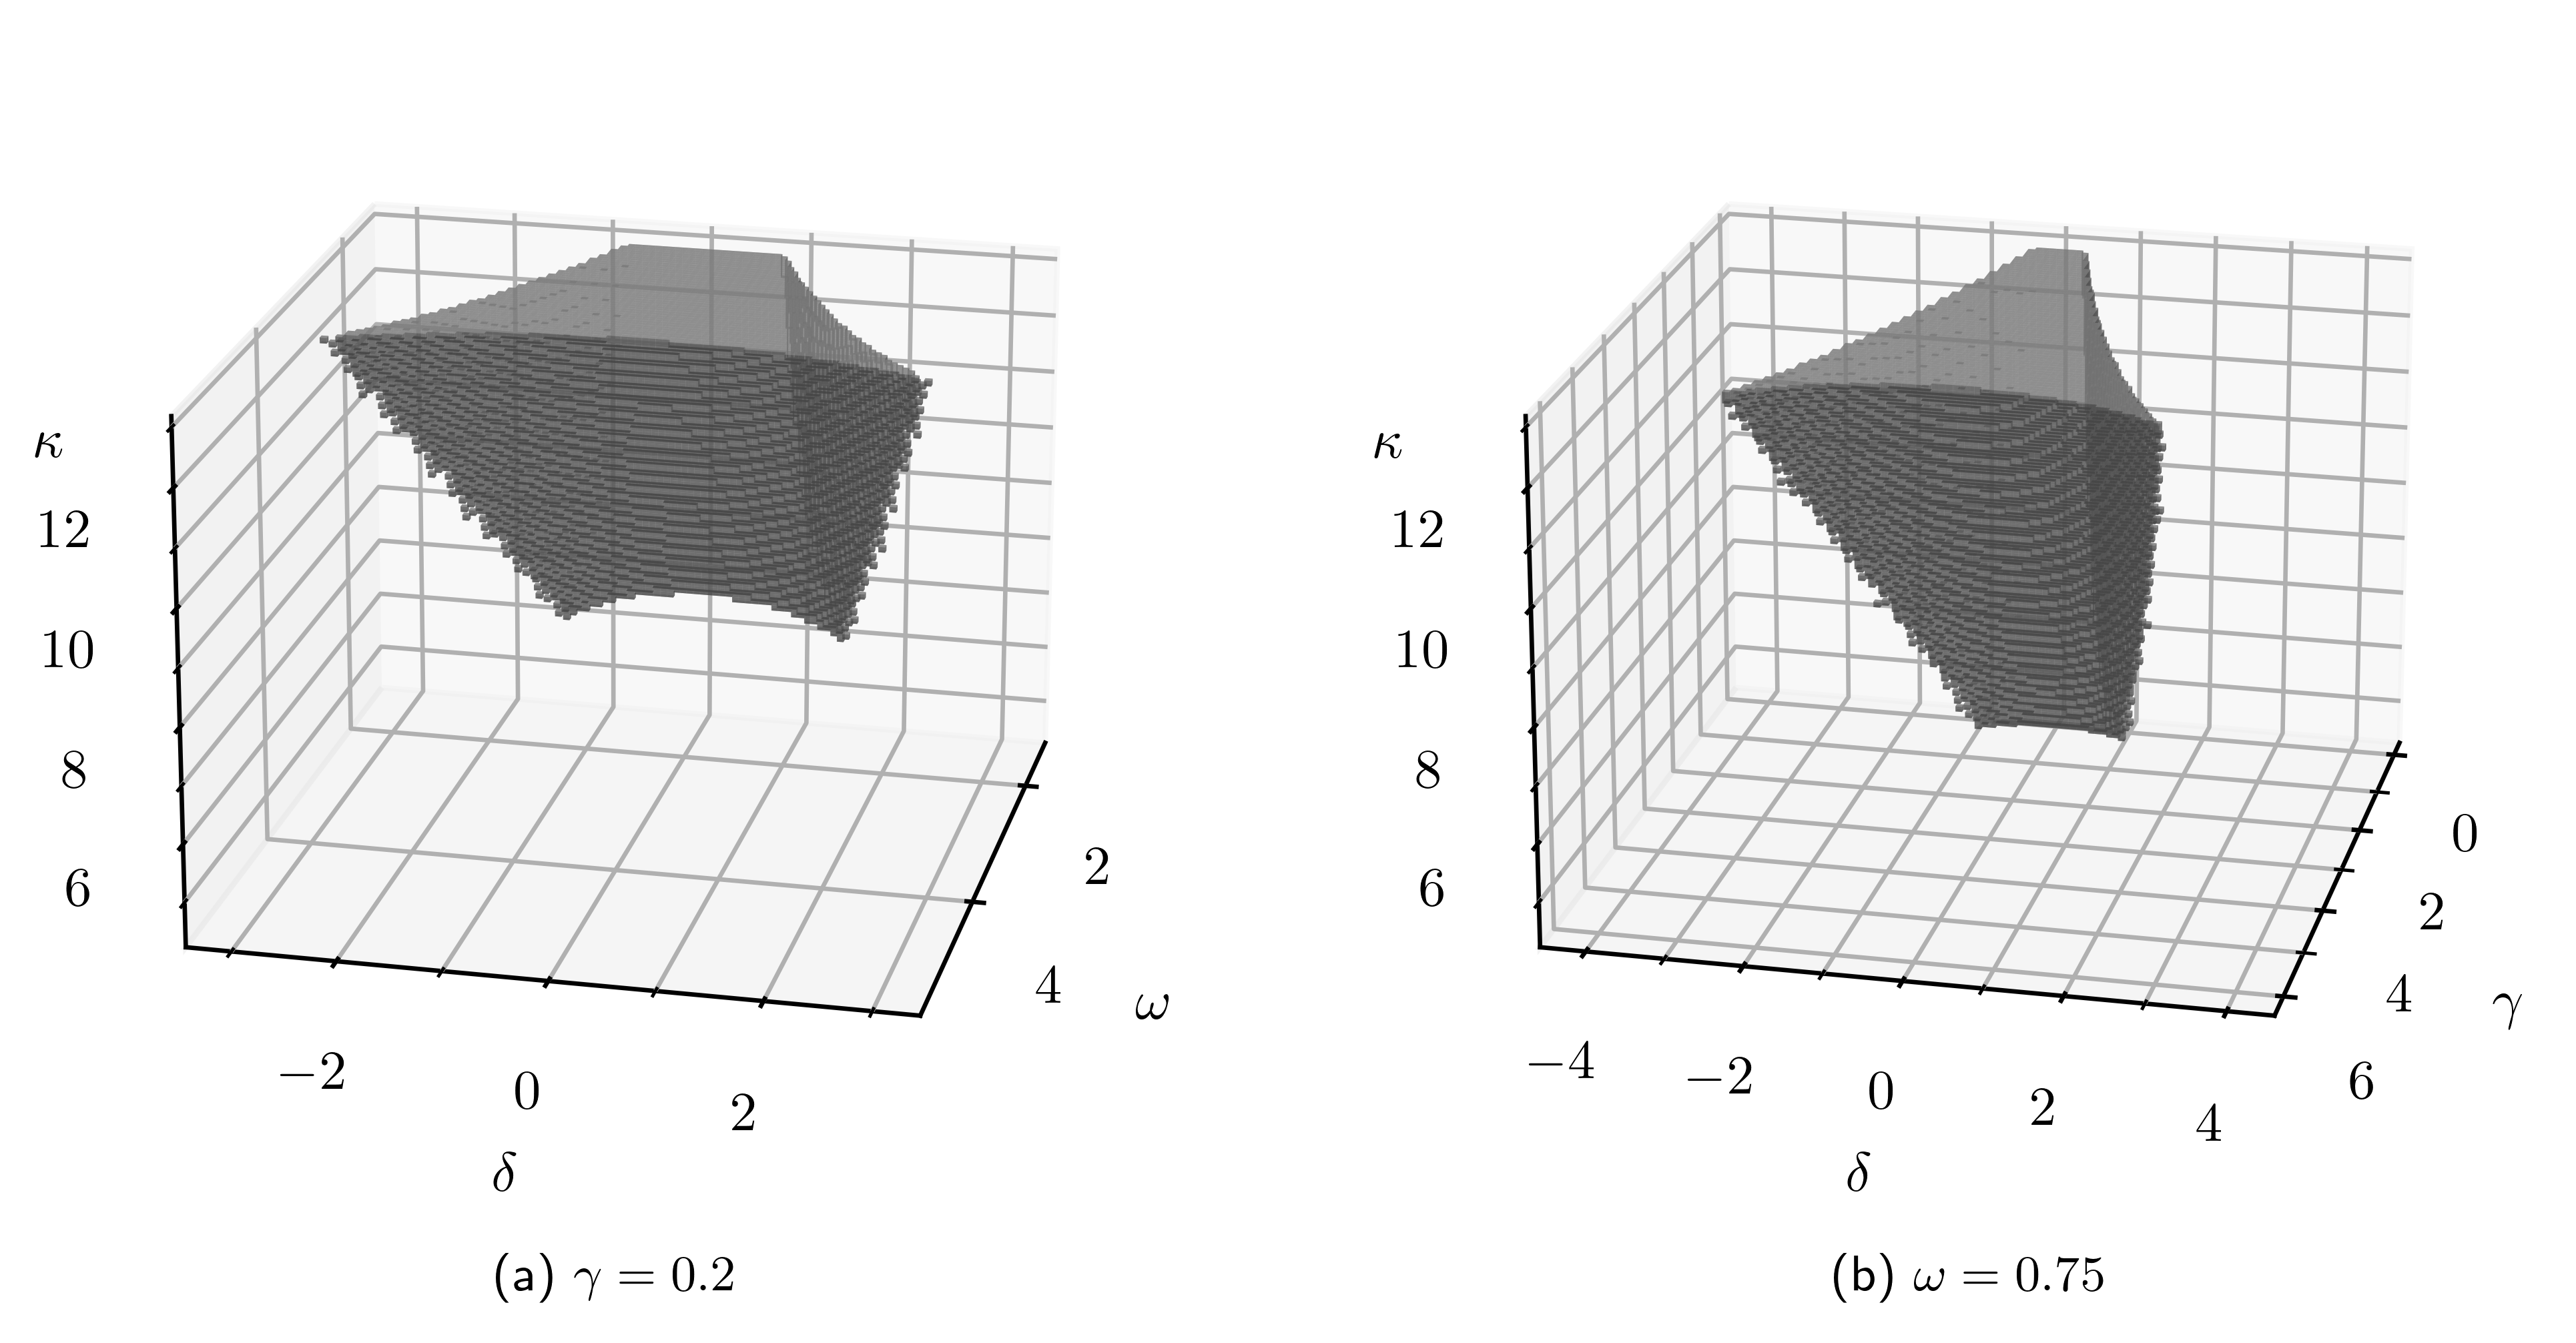
\includegraphics{pictures/numb_of_fixp_stab3d_gw.png}
    \caption{The gray filled region has 3 fixed points, whereas the rest of the shown parameter space has 1 fixed point. In the left graph $\gamma$ is held on $0.2$, where in the right graph $\omega$ is fixed to $0.75$. The two parameters $\omega$ and $\gamma$ shape the regions of different numbers of fixed points similarly.}%Shown in the bottom row are different projectin views. They do not show cuts through parameter space, but projections of one parameter dimension onto the other two. I find this gives a better impression of the shape of the area with three stationary solutions.}
    \label{fig:numb_of_fixp_3D}
\end{figure}
The stability of the stationary solutions is also determined analogously to the zero detuning case. The equations of motion are linearized in the fixed points and the sign of the eigenvalues of the linearization is evaluated. The findings of this analysis draw a consistent picture with the one found for $\delta=0$, as shown in \figref{fig:stability_of_solutions}. Stable stationary solutions exist and complement the zero detuning case. But contrary to this case, here there also exist regions, where no stable fixed points are present. In these parts of the parameter space more complicated behavior is expected, as for example limit cycles.
\begin{figure}[H]
    % \vspace*{-1cm}
    % \centering
    \hspace*{-1.2cm}
    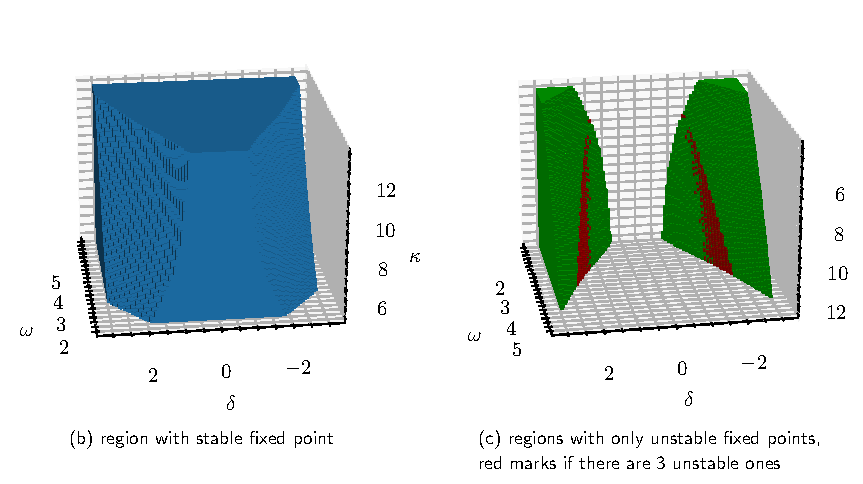
\includegraphics{pictures/stability_regions_2plots.pdf}
    \caption{Stability of the stationary points. The blue filled area has one stable fixed point, whereas in the green filled region there is no stable fixed point at all. One can also find a regime, in which there are three fixed points, but all of them are unstable. This area is marked red. Pumping and dephasing are set to $\Gamma=1$ and $\gamma=0.2$.}
    \label{fig:stability_of_solutions}
\end{figure}

\begin{figure}[H]
    \vspace*{-0.3cm}
    % \hspace*{-1.2cm}
    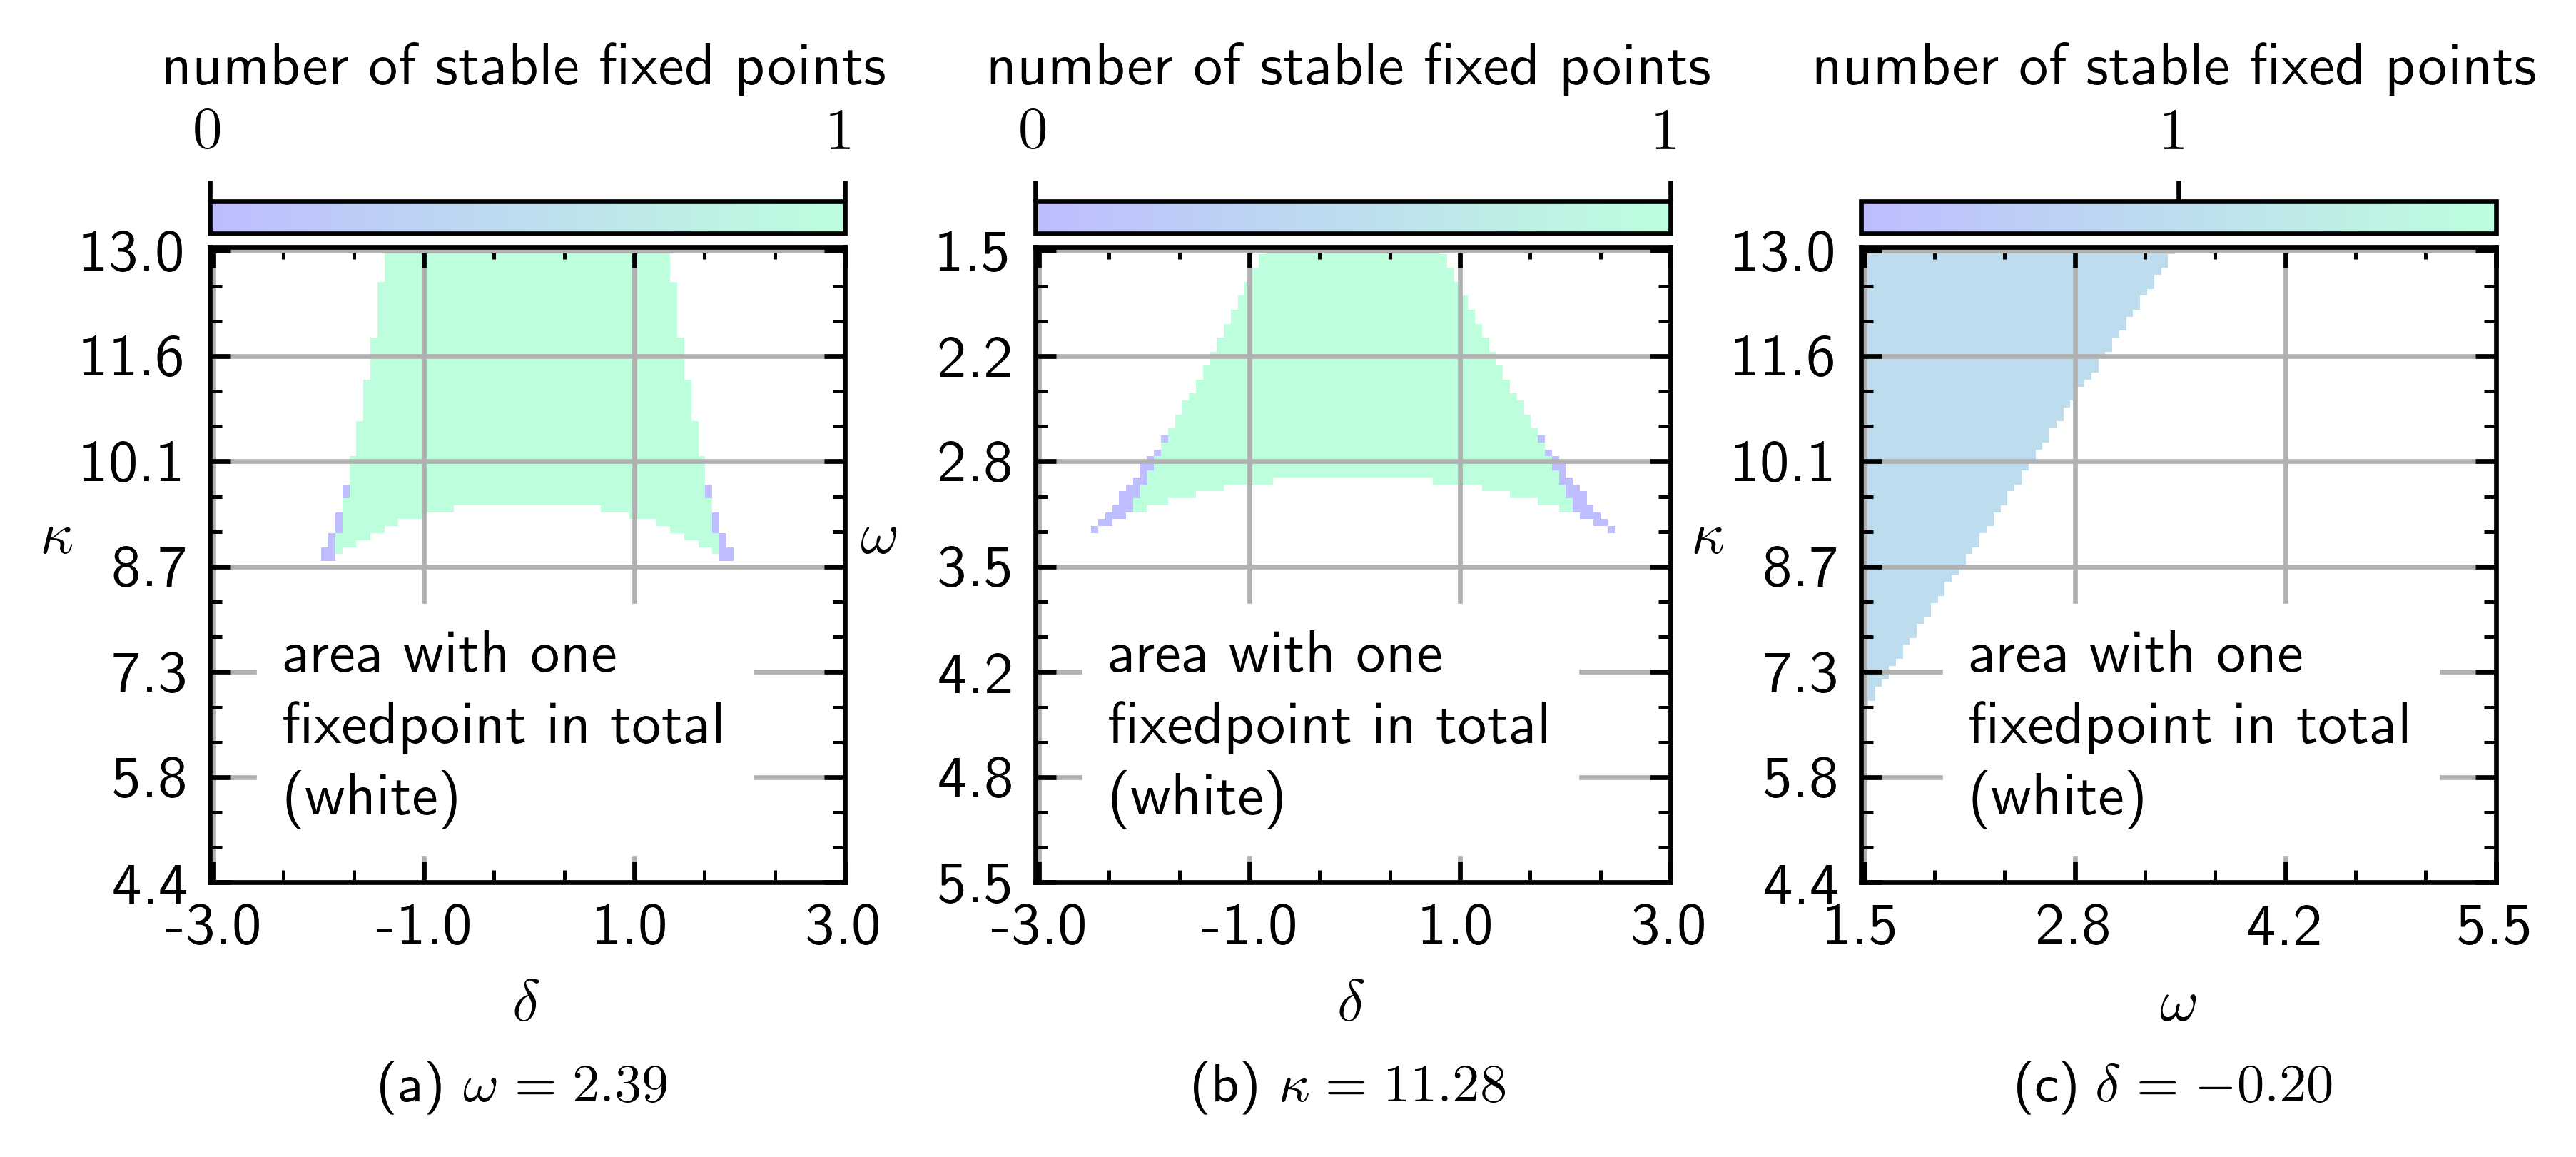
\includegraphics{pictures/numb_of_fixp_stabcuts2.png}
    \caption{Stability of the three stationary points. In this diagrams the area, in which three fixed points exist, is evaluated in more detail. Thus marked white is the region, where only one fixed point is present, without distinction between stable and unstable ones. The purple sections indicate parameter constellations, for which there are 3 fixed points, but all of them are unstable, whereas green ((a)-(b)) and blue (c) indicate at least one stable fixed point. The diagrams are cuts through parameter space.}
    \label{fig:stability_cuts}
\end{figure}
In \figref{fig:stability_of_solutions} a region can be noticed, where 3 fixed points exist, but all of them are unstable. This is a consequence of the fact that for increasing $\kappa$ the number of stable fixed points decreases but at the same time the total number of stationary solutions grows. \figref{fig:stability_cuts} shows that those regions are located on the surface of the area with 3 stationary points, indicating a straight forward succession of phases, as parameters are altered.\\\\
Because the treatment of different coherent dephasing strengths does not deliver additional insights, I will only consider a fixed dephasing at $\gamma=0.2$. A short treatment for varying $\gamma$ can be found in \appref{appendix:stability_gamma}.
% \begin{figure}[H]
%     \floatbox[{\capbeside%\captionsetup[capbesidefigure]%{labelsep=newline}%
%     \thisfloatsetup{capbesideposition={right,center},capbesidewidth=none}}]{figure}[\FBwidth]
%     {\caption{A 3D depiction of the area of 3 existing fixed points and their stability.\\\\
%     Marked with a color are the parameter configurations, where three stationary points exist. The Turquoise region at the edges mark non-stability. This shows that those parameter points lie on the surface of the region with three stationary points, and do not reach into the bulk of at least one stable fixed point, that is marked with a blueish purple. \\\\The assumption that in the absence of a stable stationary solution limit cycle can occur is in fact true. Through integration of the equations of motion one finds in those regions limit cycle and even quasi-periodic behavior. Some exemplary trajectories are found in the appendix.}}
%     {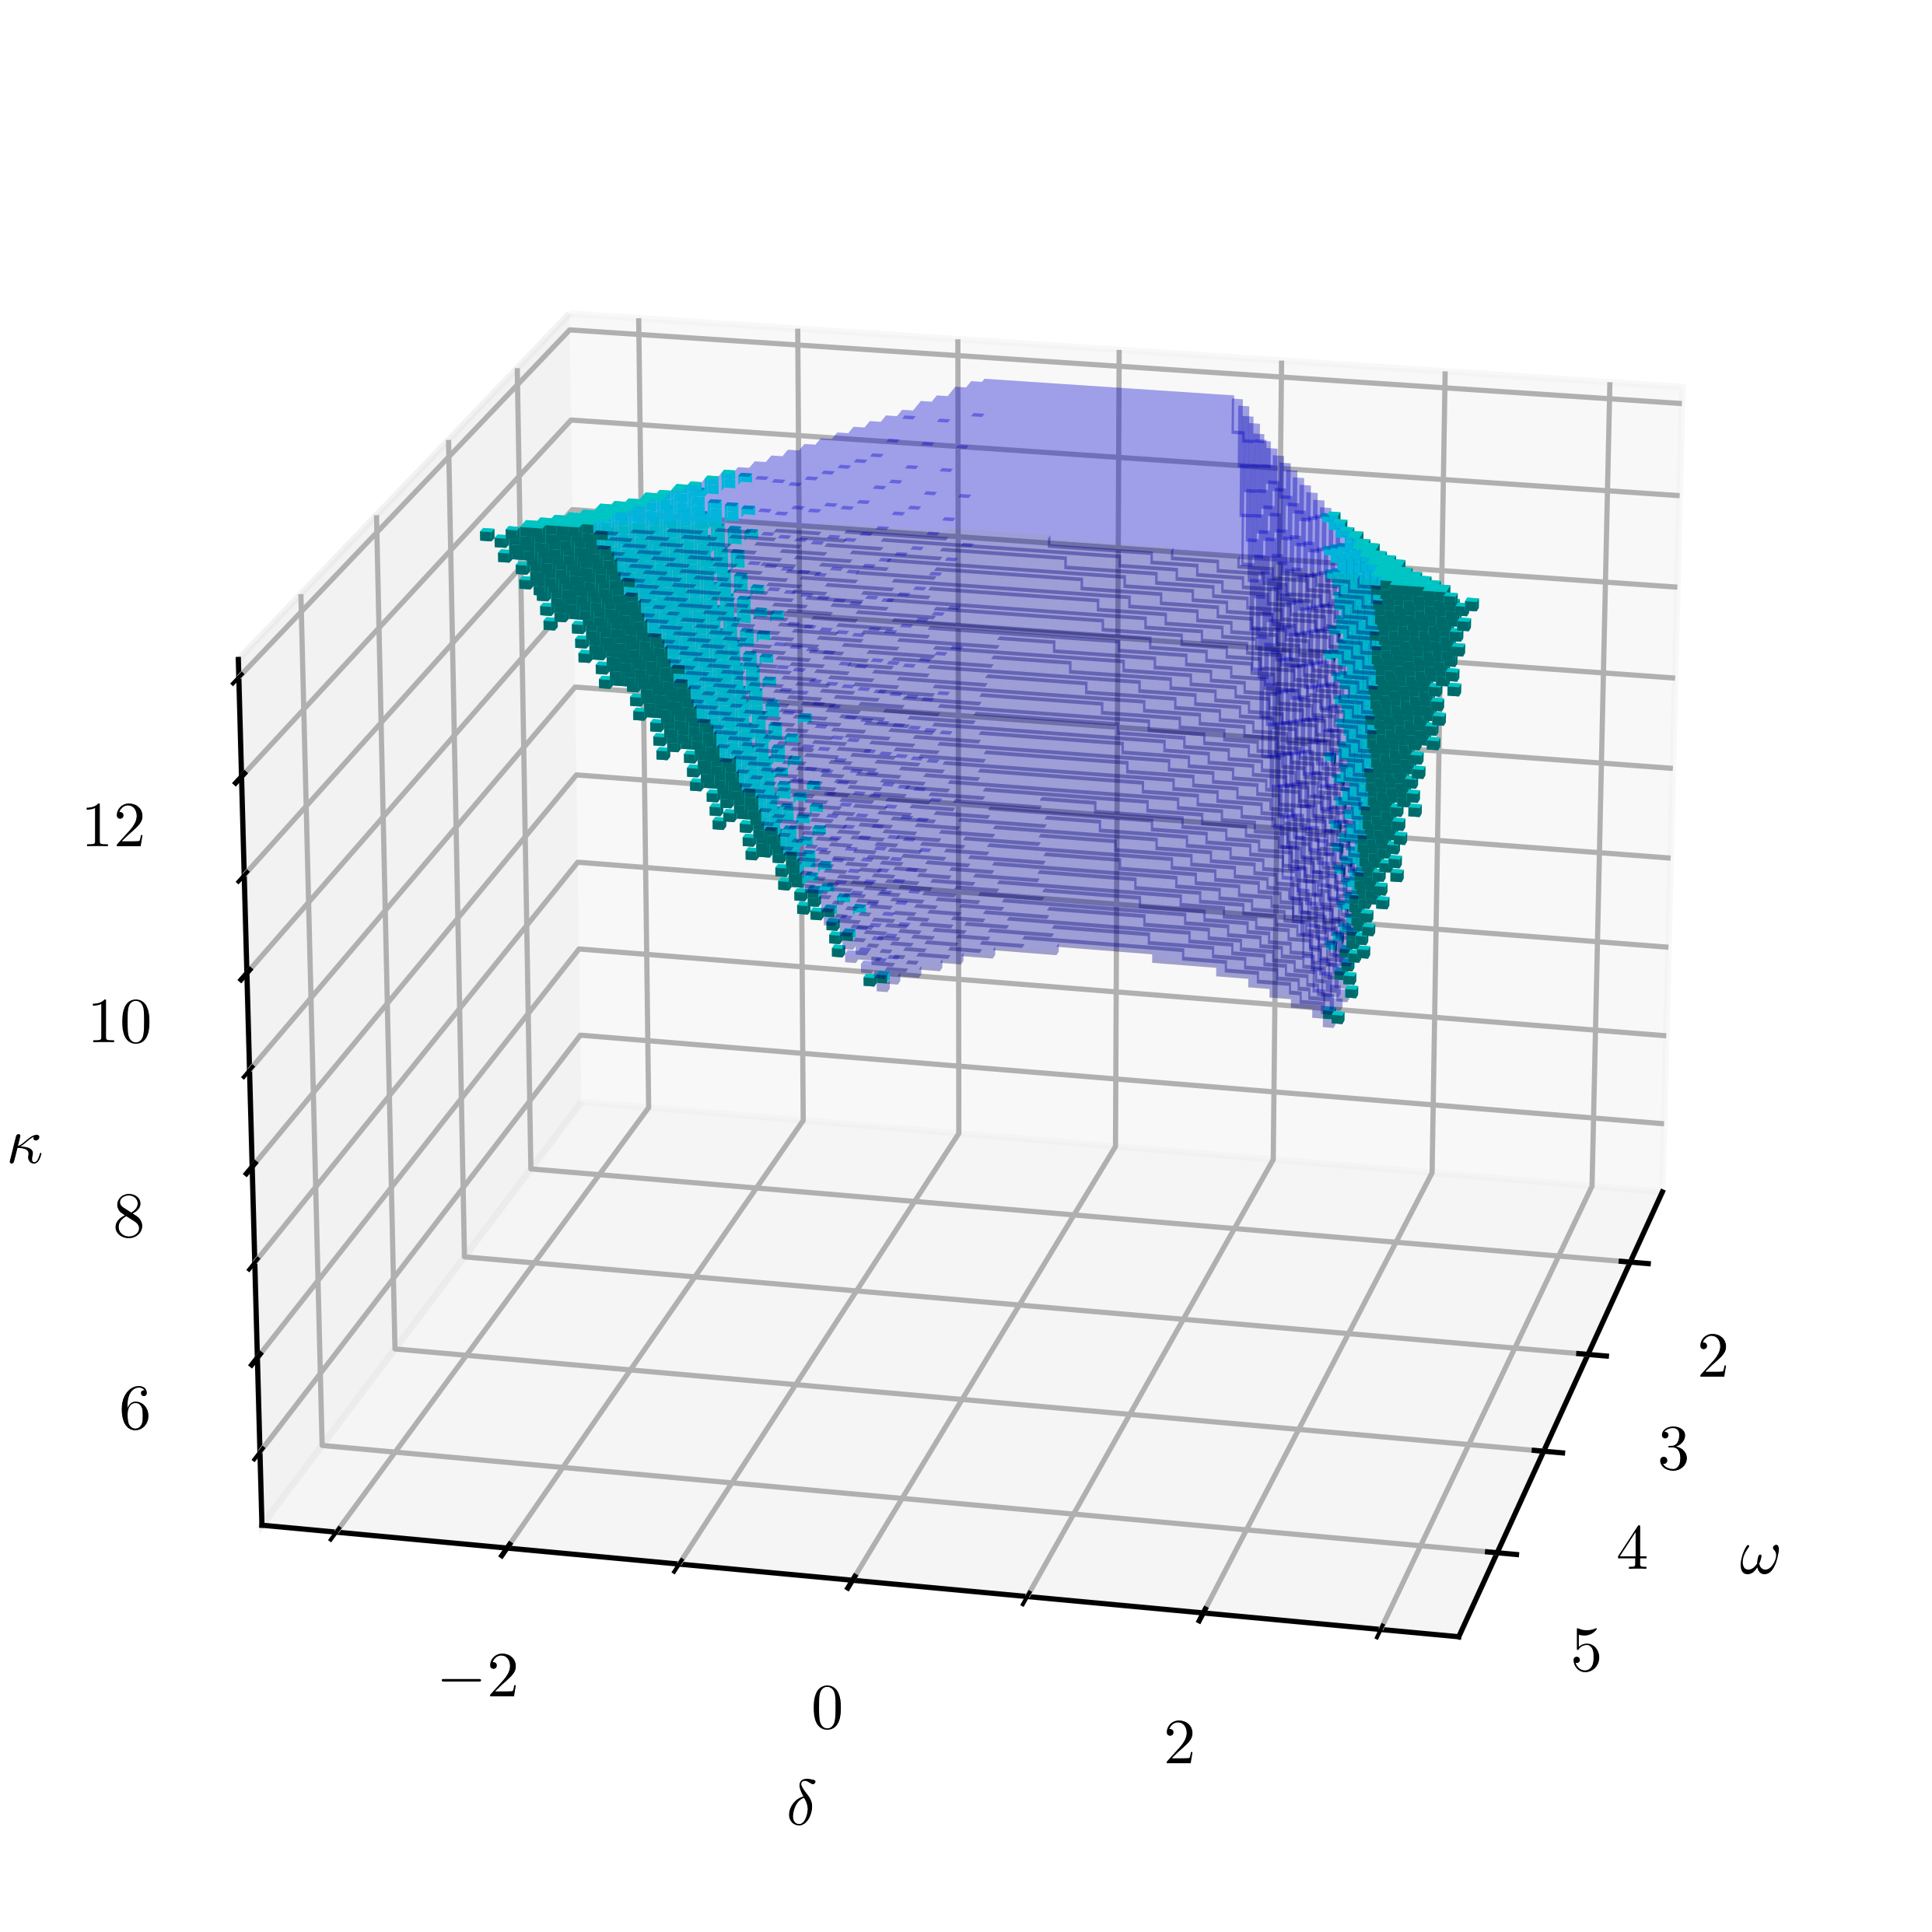
\includegraphics[scale=0.8]{pictures/numb_of_fixp_stab3d.png}}
%     \label{fig:fixp_stab3d}
%     %{\label{fig:num_of_fixp_criterium_BF}}
% \end{figure}
% \\\\
\subsection{Long-time behavior}
For long observation times the system will most likely be found in an attracting state, as already explained in \secref{sec:longterm_zerodel}. This can be a stationary solution or among others a time crystal state, meaning an undamped oscillation. Such states are in fact observable in our mean-field approach. 
\begin{figure}[H]
    % \vspace*{-1cm}
    \hspace*{-1.2cm}
    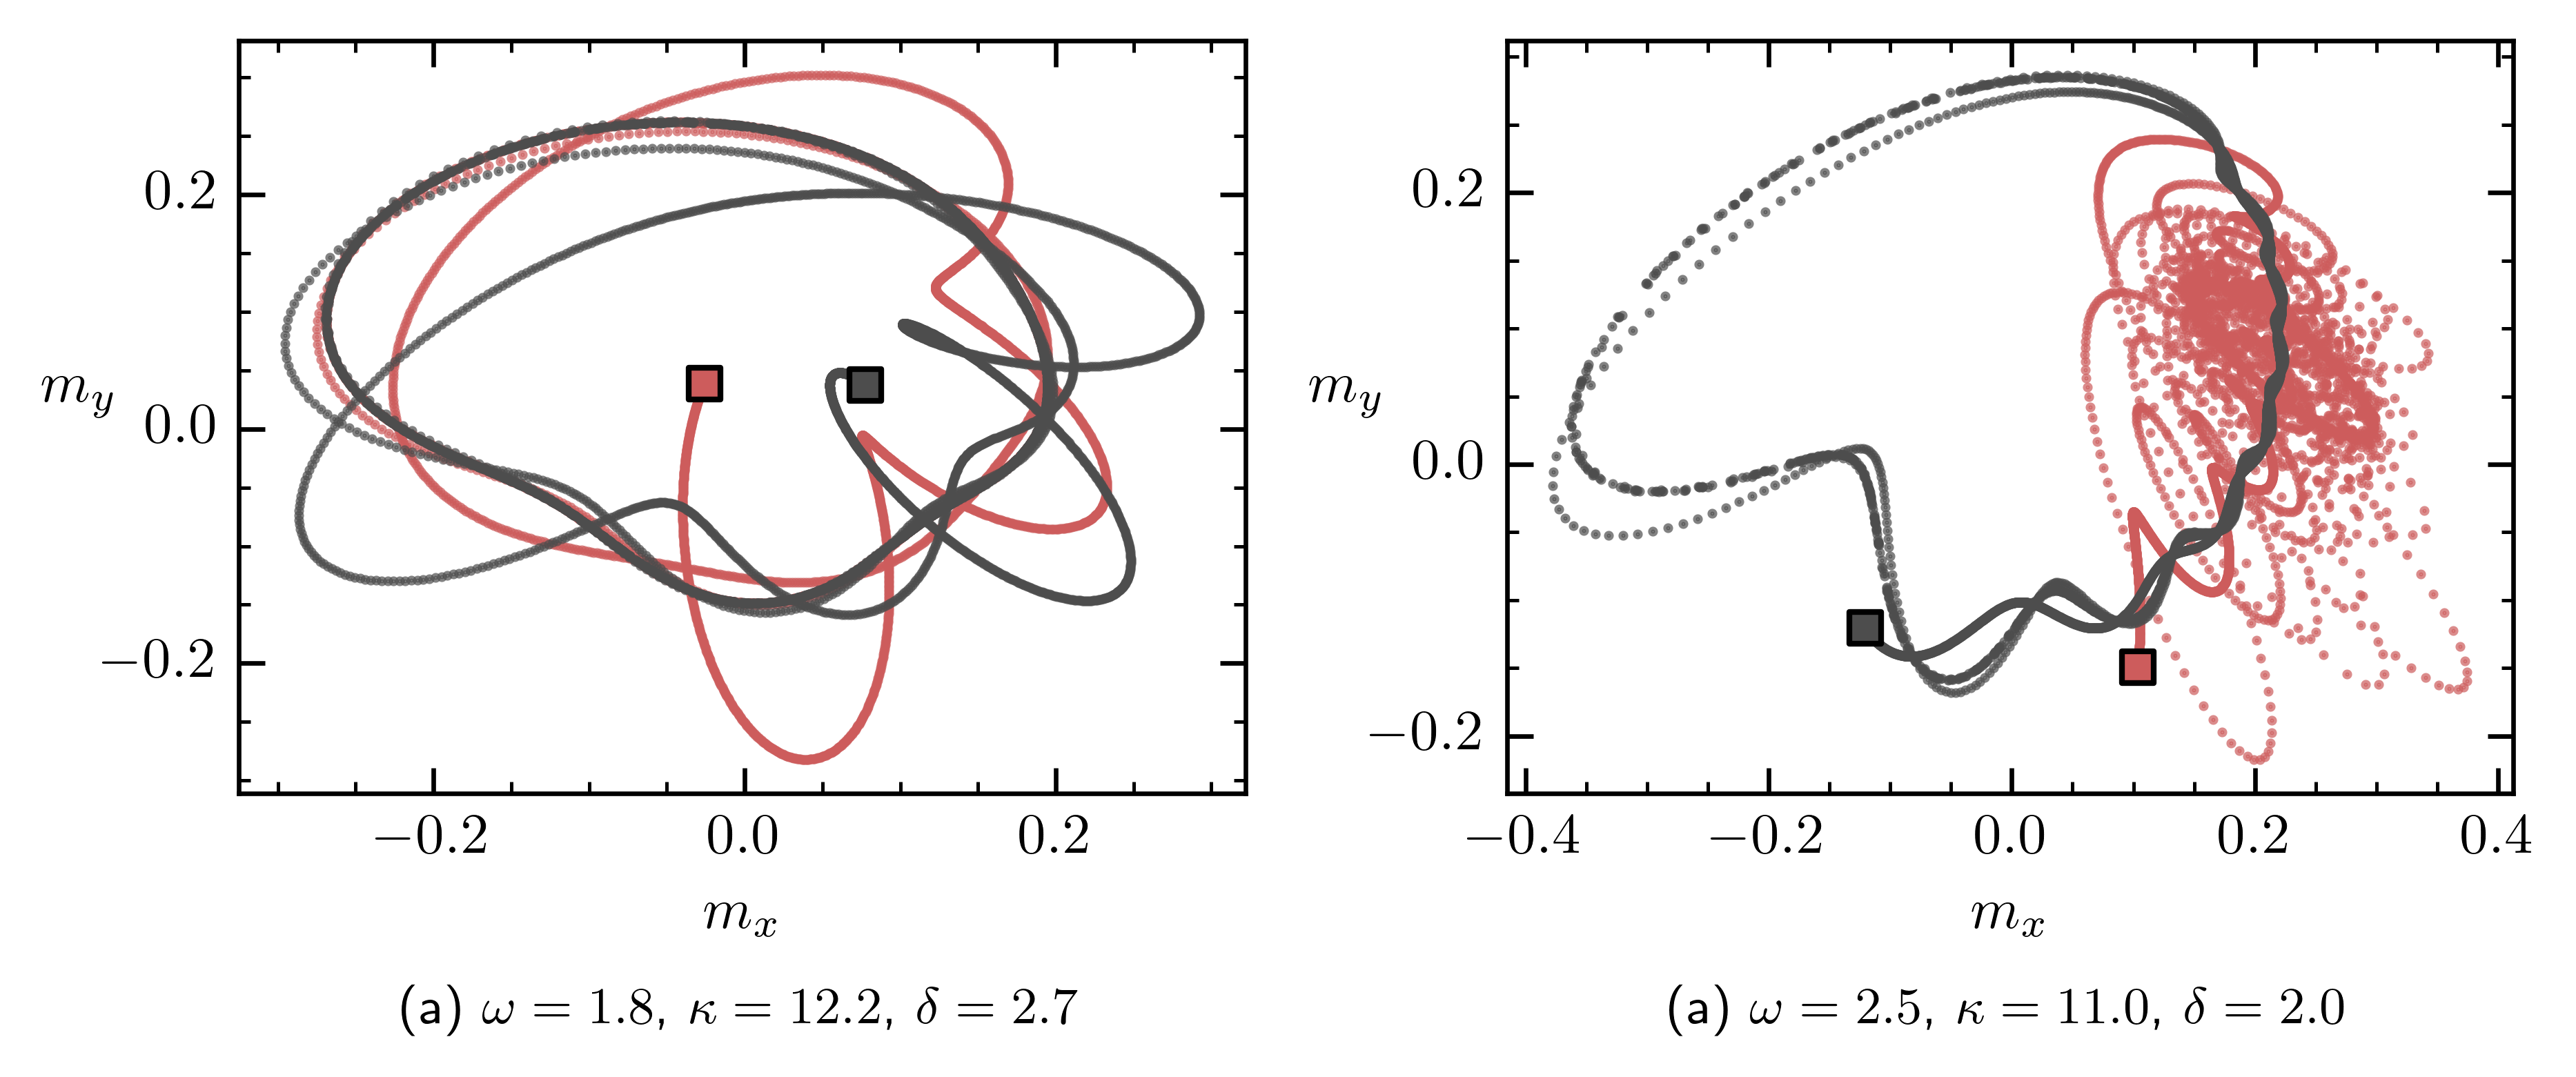
\includegraphics[scale=1]{pictures/lc_example.png}
    \caption{Two exemplary trajectories for two different parameter configurations. The starting points were picked randomly. The small squares with the black frame indicate the starting points of the system.}
    \label{fig:expl_lc}
\end{figure}
In \figref{fig:expl_lc} I plotted two exemplary trajectories for two different parameter configurations respectively, starting at a random initial state of the collective spin. In \figref{fig:expl_lc} (a) one can see that after a convergence time both trajectories overlap each other. So there is only one limit cycle that the system is drawn to for both starting positions. Of course the phase of the oscillation depends on the start and can be different. But the trace of the trajectories in spin space coincides for long times. \\\\For the parameter configuration in \figref{fig:expl_lc} (b) at least two distinct patterns are possible for long times. The gray trajectory converges relatively fast to its limit cycle and hence looks cleaner. The rather messy appearance of the red trajectory stems from the long time it takes to approach its final long-time state. But both trajectories converge, as I have checked. In fact the darkest and broadest shaped ellipse that can be seen in red marks the limit cycle to which the trajectory converges.\\\\
The fact that two different limit cycles are possible states for long times tells us that the system exhibits multistability for certain parameter constellation, in form of the presence of more than one attracting state. Where the system eventually ends up is determined by the state at the beginning of the dynamics. In \appref{appendix:expl_traj} a few more exemplary long term states of the system are depicted for different parameter configurations.\newpage
The remaining part of this section is devoted to a further analysis of the evolution of multistability in parameter space and how the possible long-time states change with changing coupling constants. I will also be able to map some of the properties onto the language of synchronization.\\
A simple way to track the change of limit cycles as well as the rise of multistability is to observe the mean value of a limit cycle over its period.
\figref{fig:fixedpoint_colormap} has been created by plotting the stable stationary solution, where it exists, and in the other case the average over a period of a limit cycle.




% When examining the long term behavior of a system, a general point of interest is how the eventually occupied states shift and deform, when the parameters are changed. A simple observable in the context of time crystals is the mean value over a period of the limit cycle. 
\begin{figure}[H]
    % \vspace*{-1cm}
    \hspace*{-1.2cm}
    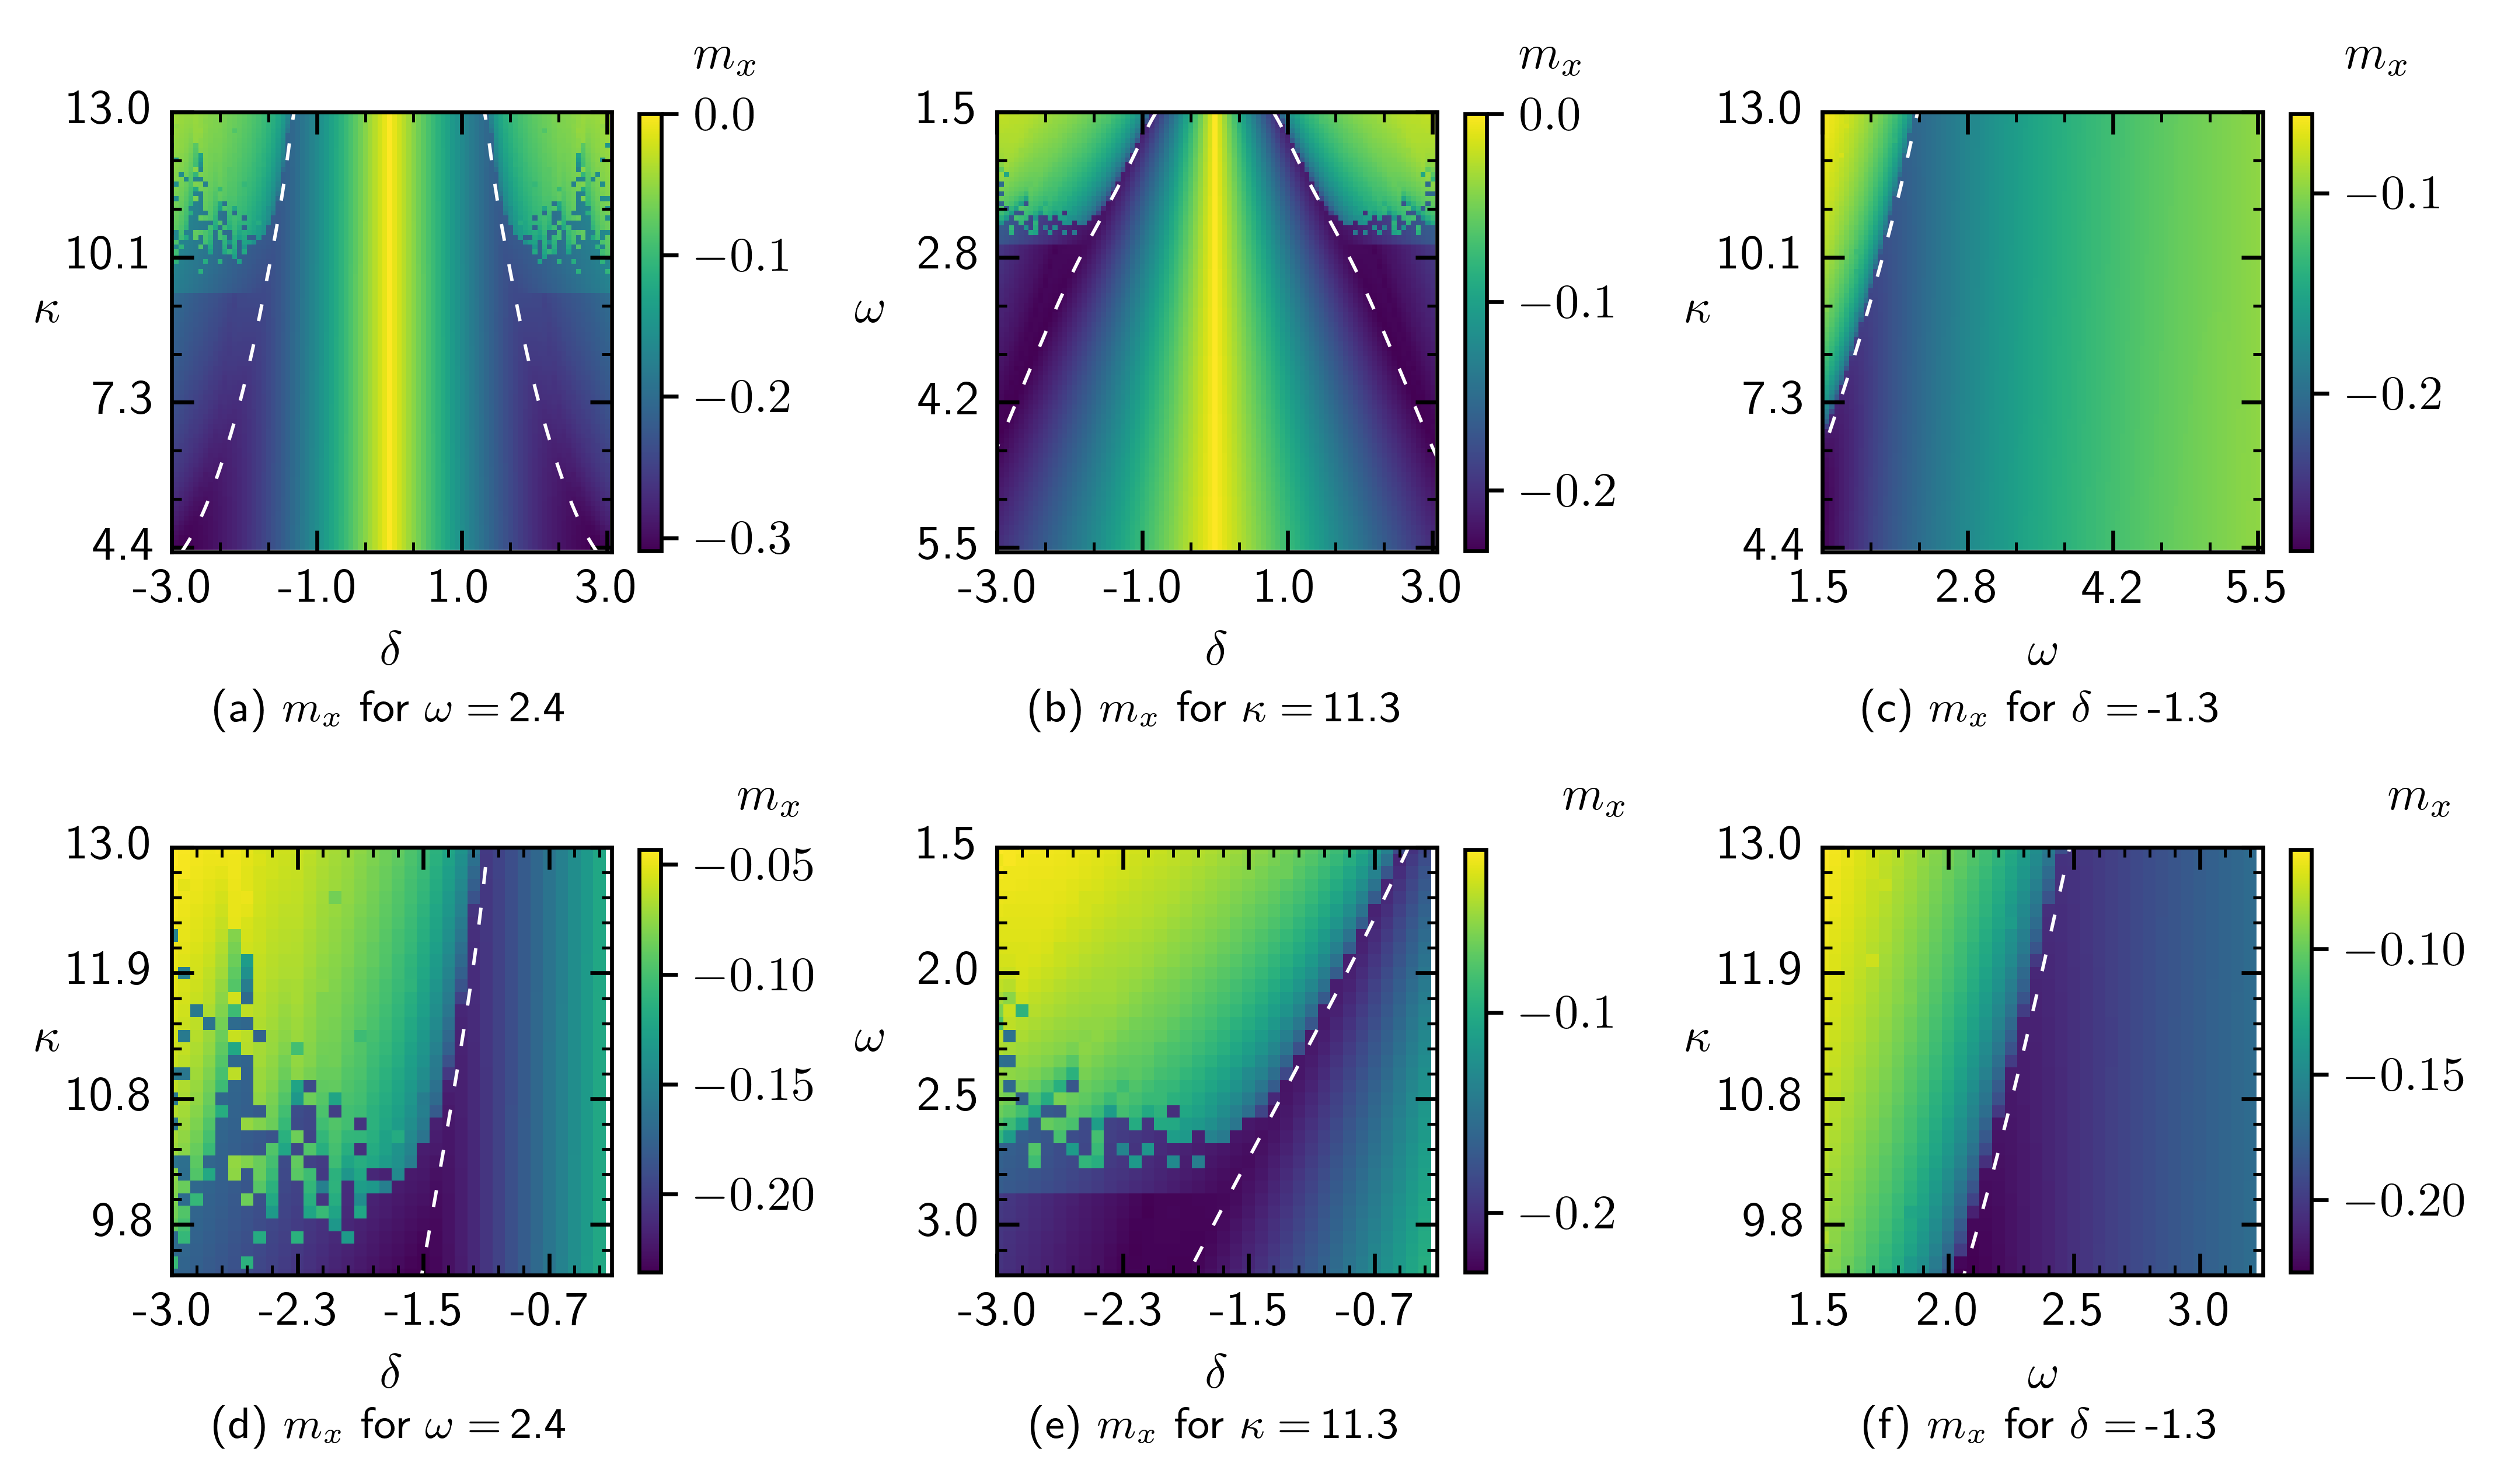
\includegraphics[scale=1]{pictures/stable_fixp_extended_withline_dashed.png}
    \caption{Shown is the $m_x$ component of the stable stationary points and of averaged limit cycles for different cuts through parameter space. Under each cut in the top row is a close-up of the interesting areas in the top left corners. the white dashed line separates the regions with one and from those with no stable fixed point. In the cases where more than one limit cycle exists, I chose the one whose average had the smallest $m_x$-value.}
    \label{fig:fixedpoint_colormap}
\end{figure}
By examining \figref{fig:fixedpoint_colormap} one can tell that the transition from stationary steady states to the time crystal phase, which is marked by the white dashed line, is at some parameter points more smoothly than at others. The separation line has been computed by selecting the first point where there is no stable fixed point anymore, when passing through each line of the evaluated parameter grid in decreasing order of $\delta$. A polynomial of 4th degree is then fitted to those points to approximate the border line. Notice that as a result of this method the separation line lies inside the time crystal phase. Also because of the approximate nature of this determination, the line should only serve as a orientation, where the phase separation is located.\\\\
For the cuts with constant $\kappa$ and constant $\omega$, the area where limit cycles exist can be roughly divided into two regions. For one region, as already mentioned the transition from the stationary phase is very smooth, whereas for the other region, there is significant change in the average value of the long-time states to the nearby parameter configurations where stationary solutions exist. Multistability has also its influence on the appearance of the diagram. Where it occurs, I plotted in \figref{fig:fixedpoint_colormap} the averaged limit cycles with smallest $m_x$-value. \\What also stands out is that the phase plot in this part of the parameter space is very fragmented. The biggest reason for this fragmentation is that for the generation of this diagram too few starting points have been chosen to detect all present limit cycles. Another important factor was, that in order to integrate up to long times without having too much error, one has to choose the precision of the integrator very high, which has not been done, when originally generating \figref{fig:fixedpoint_colormap}. \\Because of the high numerical expense it takes to determine enough trajectories of the system up to a sufficiently large time with good precision, I have decided to redo the diagram in more detail only for a selected area in the plane of $\omega=2.3889$ (\figref{fig:precise_multistab2d}). An additional remark has to be made regarding \figref{fig:fixedpoint_colormap}. In some of the plots a sudden but slight jump in the color map is noticeable. This stems from the fact that already in those plots a minor adjustment of precision has been made for the critical regions. %The white dashed separation line between limit cycles and stationary points has been determined by collecting the border points where just no stable stationary point exists anymore and fitting a spline to it. Because of the low resolution of considered parameter constellations the curve should serve more as an approximate locater of the border between limit cycles and fixed points than a definite cut.
\subsubsection{Synchronization}\label{sec:synchronization}
Despite all of the mentioned constraints, the diagram is valid for most of the shown area, as only the change from the one limit cycle phase to the multistability region has some artefact. Thus I will focus now on the information that can be retrieved from the valid parts of the diagram.\\%, due to the above mentioned reasons. 
The shape of the white dashed separation line in the $\omega$-$\delta$-diagram reminds of the typical division of states for contexts in which synchronization effects are observable. As mentioned in the intdroduction, synchronization is the adaption of oscillating systems to each other, which are coupled through a weak interaction. In our case the two synchronizing parts are the system on the one hand and the driving laser on the other. As the driving laser is not affected by the system, only the latter can adapt. Hence synchronization takes place when the system oscillates with the same frequency as the laser. As the equations of motion are formulated in the rotating frame of the laser, see \secref{sec:theory}, the dynamics in case of frequency locking take the form of stationary points. A few conditions have to be met in order to being able to speak of synchronization \cite{pikovskij_synchronization_2007}:
\begin{itemize}
    \item The coupling between the two systems has to be weak enough to speak of non-trivial influence.
    \item Both systems have to be able to maintain autonomous oscillations, if decoupled.
    \item If the original frequency of one of the systems is altered, this has to have an effect on the resulting common frequency, that arises due to the coupling.
\end{itemize}
As the both regions of limit cycles as well as stationary points extent to small values of $\omega$, i.e. small interaction between laser and system, in those areas the condition of weak coupling is satisfied. Also the last condition of changing locked frequency with change of the driving frequency is fulfilled. I have already said, that the laser in our formalism is not influenced by the system. Therefore only the system can follow the change in laser frequency. As the system exhibits stationary states in a certain interval around $\delta=0$, what has been confirmed in \secref{sec:stab_3D}, the system is locked to the oscillation of the laser for changing laser frequencies. In order to confirm autonomous oscillations of the system without laser driving, one has to remove the driving from the formalism, which is not trivial. The Hamiltonian for this case reads
\begin{align*}
    H &= \frac{\omega_0}{2}\,J_z +\alpha\,(J_+a + J_-a^\dagger)+ \beta\,J_z\,(b^\dagger+b)+\xi\,\sum_{i=1}^N\,(\sigma_i^-c_i^\dagger+\sigma_i^+c_i)
\end{align*}
As a consequence of not having to perform a transformation into the rotating frame of the laser, the bosonic ancilla operators, are defined slightly differently, i.e. related to a factor $\propto\exp(i\omega_0t)$. But this really does not change the quality of the dynamics. It becomes obvious that the same dynamics can be achieved by considering the original Hamiltonian and setting there the driving $\omega=0$ and $\delta=\omega_0$. Examining trajectories for these parameter configurations one can find that limit cycles arise. Thus the system is able to maintain oscillations even without external laser driving, hence satisfying the remaining condition for synchronization. As mentioned earlier the transition line between fixed points and time crystal phase, has a typical property of the phase locking effect. The more the frequencies of the involved systems differ, the stronger the coupling between them has to be to achieve synchronization. 
\subsubsection{Multistability}\label{sec:multistability}
Having thus found an enriching correspondence of the found phase diagram to synchronization effects, I want to turn to the discussion of multistability, that occurs in the time crystal phase. For this analysis I have redone the diagram that shows the change of the average value of a limit cycle over a period for the plane with $\omega=2.3889$. It is shown in \figref{fig:precise_multistab2d}.
\begin{figure}[H]
    \vspace*{-0.45cm}
    \hspace*{-1.2cm}
    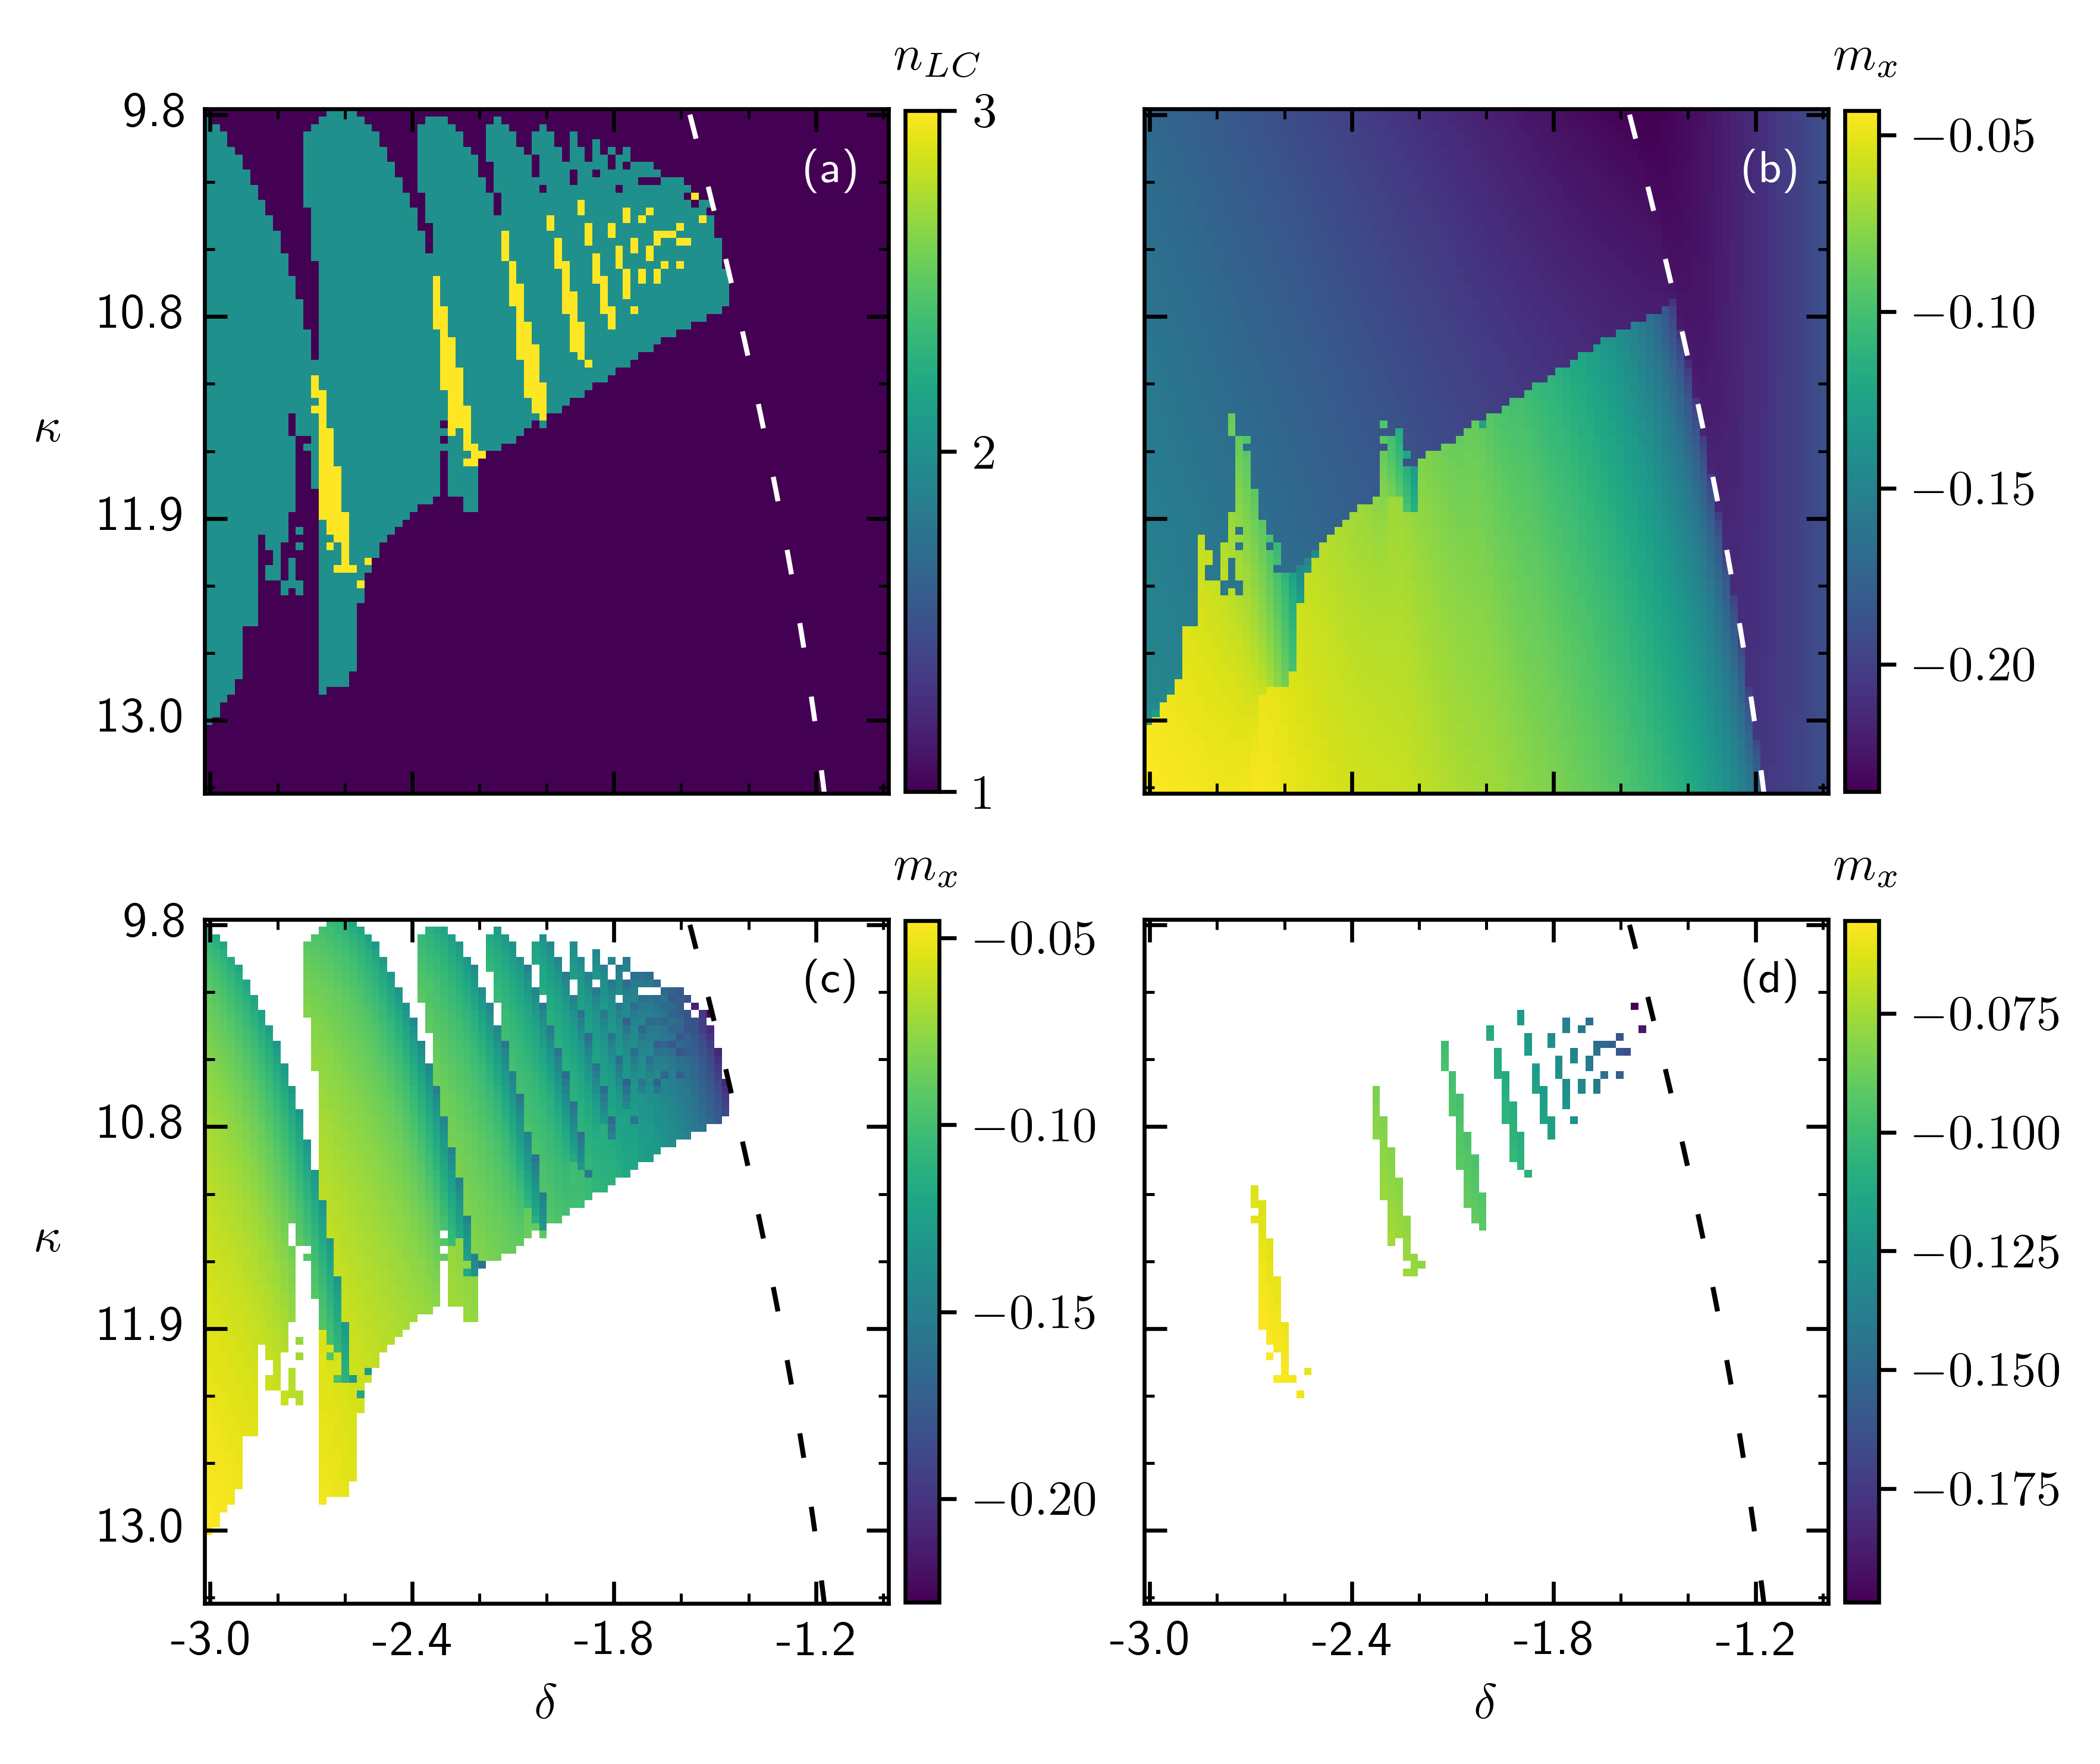
\includegraphics{pictures/limit_cycle_mean.png}
    \caption{multistability phases. In (a) $n_{LC}$ measures the number of different limit cycles. The dashed line, which is also present in the other three plots, separates the region of fixed points (right) from that where stable long-time oscillations exist (to the left of the line). The values of the fixed point as well the averages of the $m_x$-component of the spin over a period are shown in diagrams (b)-(d). The plotted averages have been chosen in increasing order of their value, i.e in (b) the smallest values of $m_x$ have been plotted and in (d) the largest.}
    \label{fig:precise_multistab2d}
\end{figure}
\figref{fig:precise_multistab2d}(a) shows the number of different limit cycles. It was determined by computing the average value of the total spin over the period of a limit cycle. The criteria by which stable oscillations have been differentiated from each other was a distance of mean total spin of at least $0.005$. It is found that up to three different limit cycles are approached for the same parameter configuration depending on the initial condition of the system. Intriguingly for some regions of the phase diagram a repeating pattern shows when the detuning is changed. Period and amplitude of this oscillation-like behavior is decreasing with shrinking $\delta$. \\\\What is also interesting is that the sharp transition in the mean value of the $m_x$-component of the spin is not due to the rise of multistability. Multistability rather accompanies the change in mean long-time spin. Passing through parameter space from small to big $\kappa$ one can say the following. Where more than one limit cycle exists, one of them keeps up the smooth course of average spin. When moving further in parameter space up to the area, where again only one stable oscillation exists, only those oscillations survive, which continue the previous course of average spin more abruptly (\figref{fig:precise_multistab2d}(b)). Hence the multistability appears at a transition in magnitude of the averaged $m_x$-value, where a region of elevated $m_x$-value stretches out a comb of additional long time states beyond a rather sharp border. I want to explicitly mention that, what the above figure suggests - namely that the comb of \figref{fig:precise_multistab2d}(c) expands the bright section of \figref{fig:precise_multistab2d}(b) - is in  fact true.\\\\
Expanding the analysis I want to look in more detail to the behavior of multistability as the detuning is changed. Therefore I picked two one-dimensional cuts through parameter space. They are marked in \figref{fig:delta_cut_traj}. One line is picked in the area where a repeating pattern in $\delta$ is observed. Another one has been selected in the area where the number of limit cycles exhibits a large incision and despite larger integration precision, the exact border could not be resolved well. \\\\
% \begin{figure}[H]
%     % \vspace*{-1cm}
%     \hspace*{-1.2cm}
%     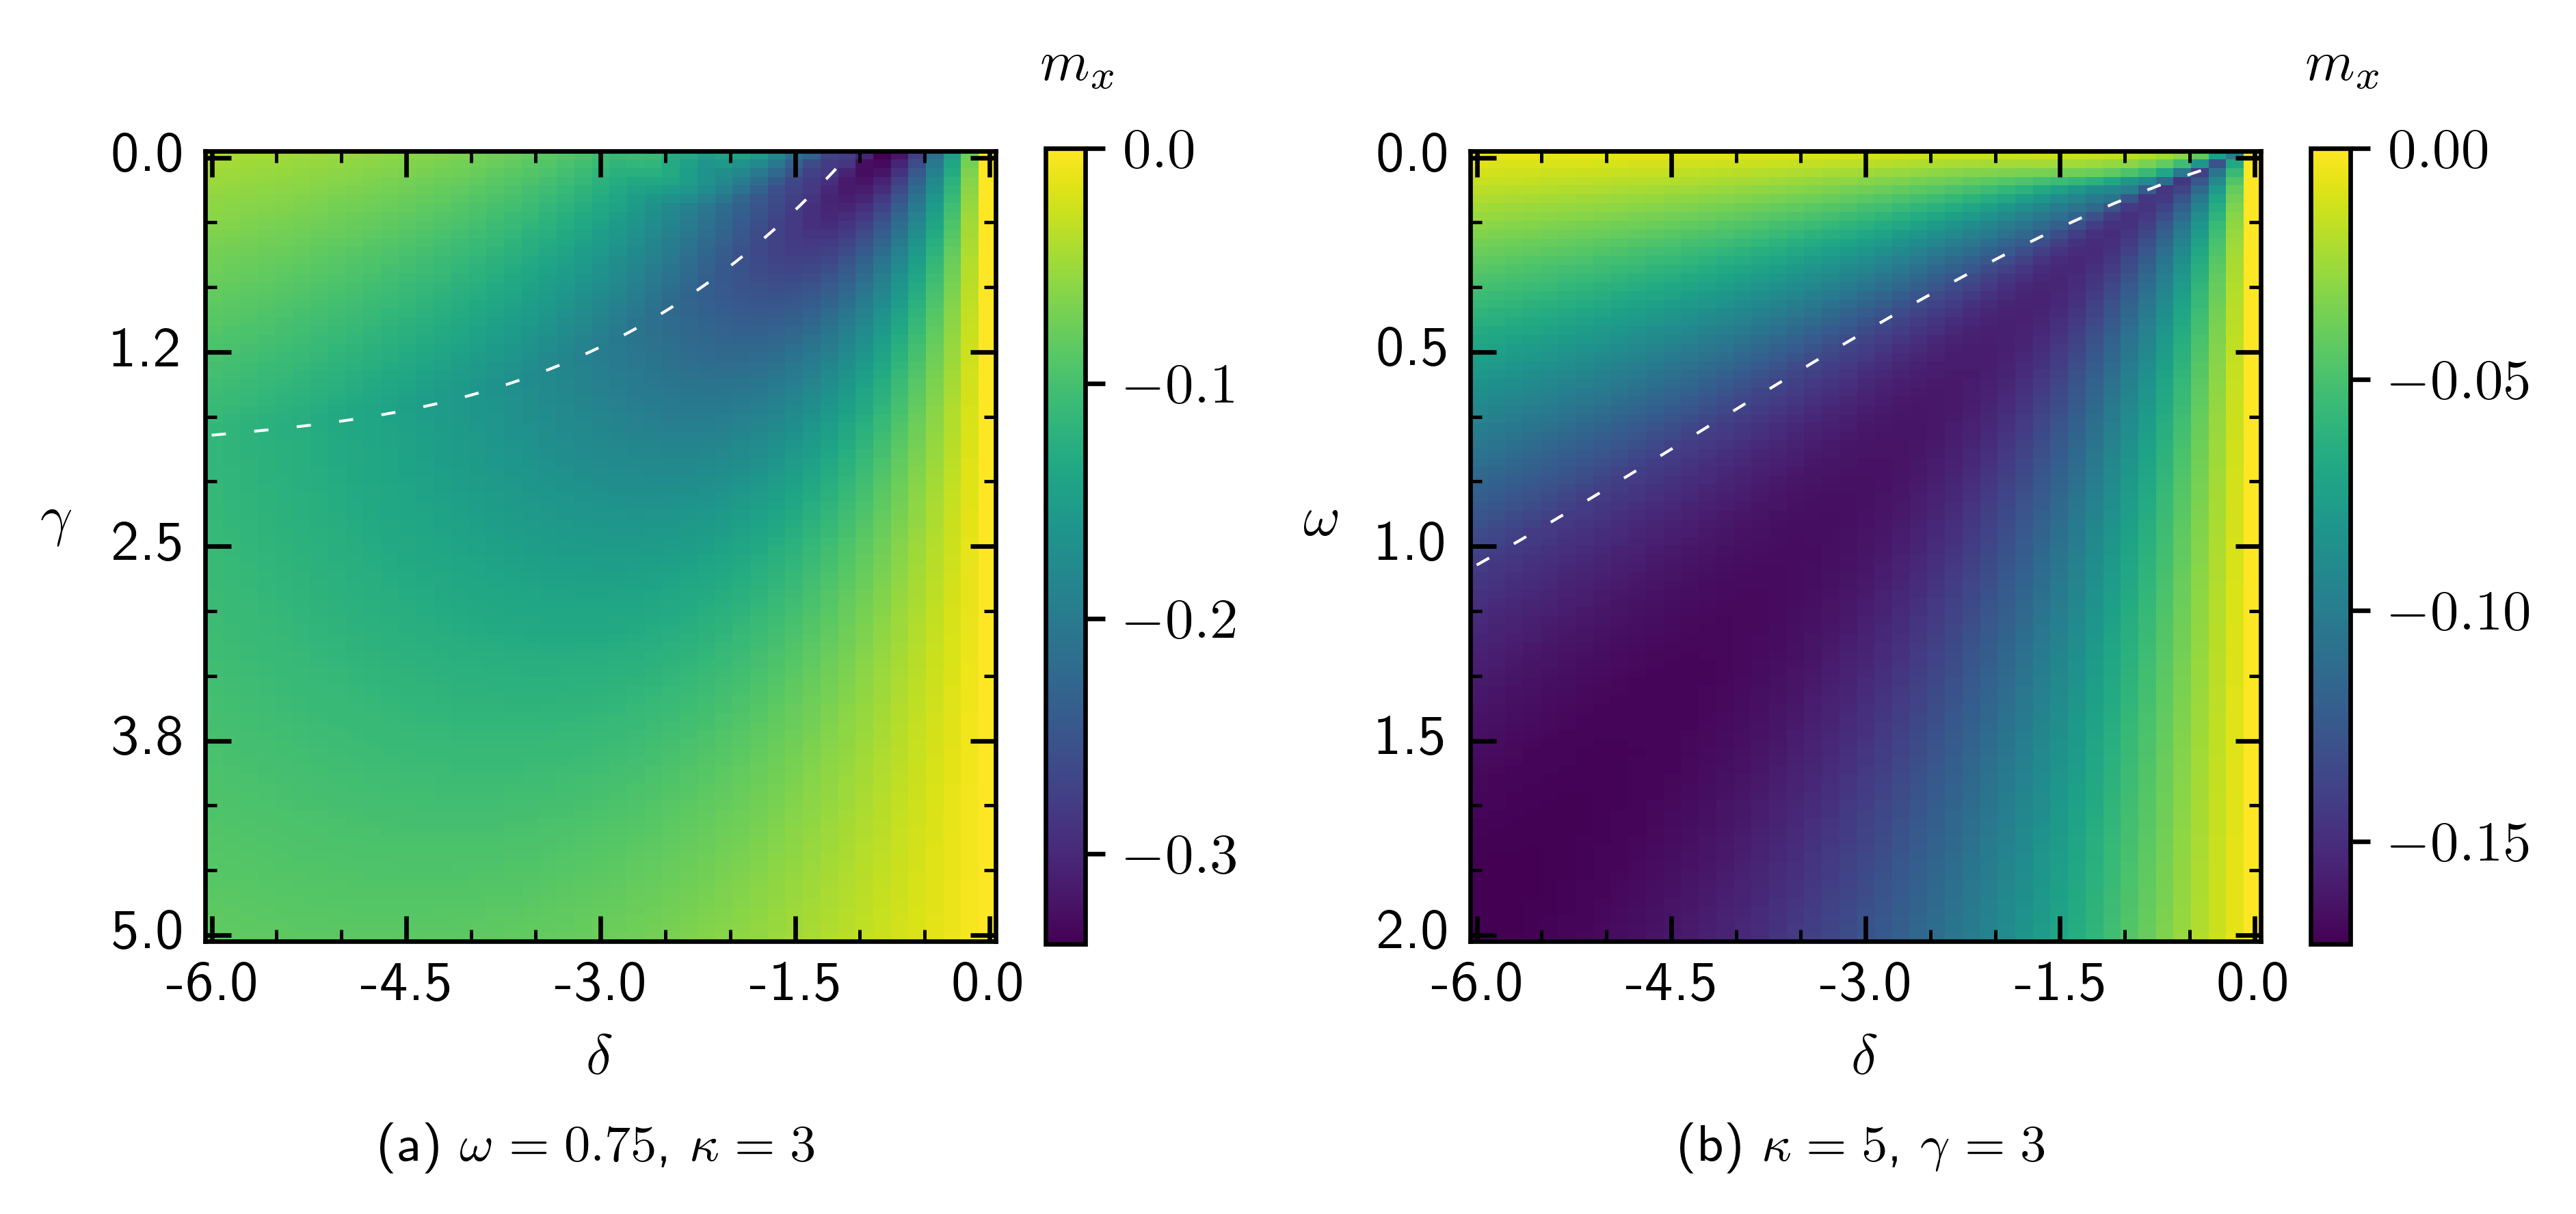
\includegraphics{pictures/limit_cycle_mean_gw.png}
%     \caption{$n_{LC}$ measures the number of different limit cycles.}
%     
% \end{figure}
\begin{figure}[H]
    % \vspace*{-1cm}
    % \hspace*{-1.2cm}
    \caption{cut locations. Drawn in white are the paths in parameter space, where the the course of multistability is examined in greater detail and resolution. The upper line has its position at $\kappa=10.12$ and the lower line is located at $\kappa=11.9$. $\omega$ has its value at $2.3889$. The white dashed line again marks the onset of stable stationary solutions for smaller detuning values.}
    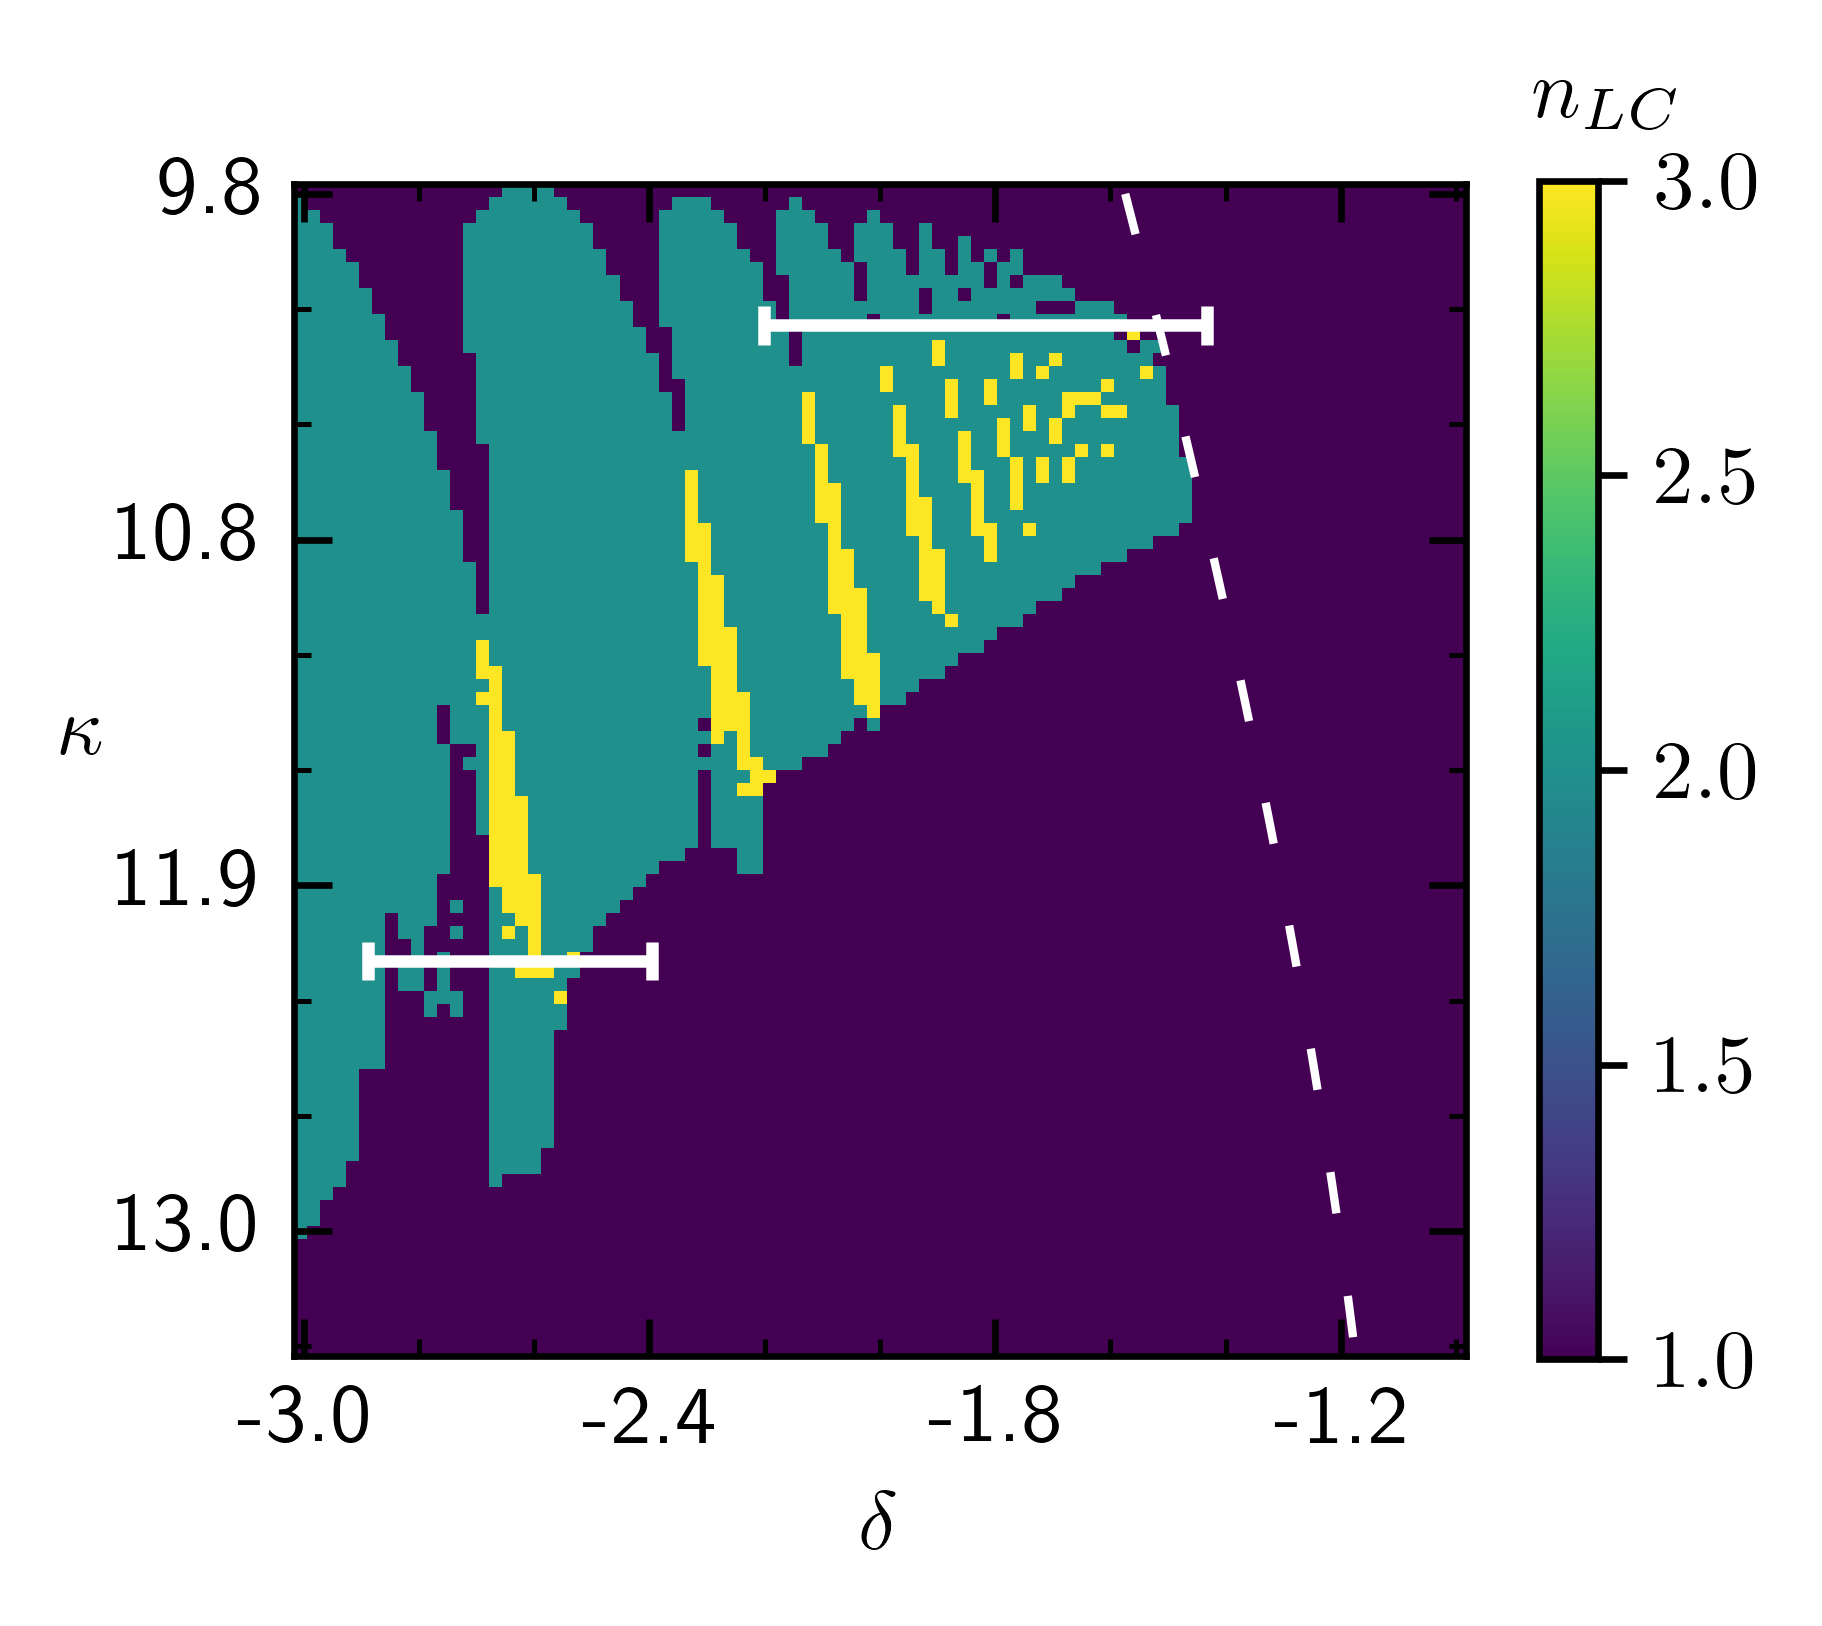
\includegraphics{pictures/multistab_cuts.png}
    \label{fig:delta_cut_traj}
\end{figure}


\begin{figure}[H]
    % \vspace*{-1cm}
    \hspace*{-1.2cm}
    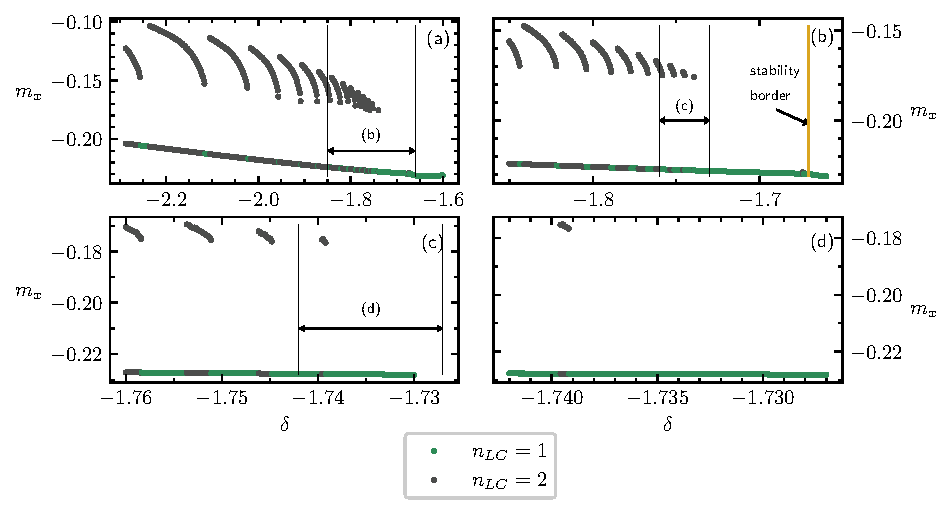
\includegraphics{pictures/multistab_line.pdf}
    \caption{One dimensional multistability cuts for the oscillatory area. Drawn are the $m_x$-values of trajectories averaged over a period of the limit cycle. In (a) 400 different values for the detuning have been considered. Particularly interesting looking sub-intervals have been identified and shown in greater detail in figures (b)-(d). All of them show the average of all the possible long-time states for 750 different $\delta$-values. Throughout the figure $\kappa=10.12$ and $\omega=2.39$.}
    \label{fig:osci_cut}
\end{figure}
The cut for the former region, where oscillatory-like patterns are found is depicted in \figref{fig:osci_cut}. It can be observed that a similar pattern repeats itself. Following the depiction of the averaged limit cycles with decreasing detuning, the distance in $\delta$ between each pattern shrinks, as well as the range of $m_x$ that each section of multistability covers. \\\figref{fig:osci_cut}(d) also shows that the pattern gets extinct at $\delta\approx-1.74$ and hence a good way before the onset of exact synchronization. I have chosen a high resolution of $1000$ values for the detuning between $-1.742<\delta<-1.727$. I expect this number of grid points to be sufficient in order to detect an additional instance of the aforementioned pattern, if it existed. But further investigation is necessary to give a final answer to this question. Another observation that can be made is that the number of fixed points jumps discontinuously in the detuning.\\\\
I want to end the discussion of multistability with the close-up that is shown in \figref{fig:delcut_bay}. It depicts a cut through the area where a wedge of singular stability is  located between two regions, in which two and three different limit cycles exist. The cut through this wedge shows highly discontinuous behavior in $\delta$. One finds two uninterrupted branches at larger $m_x$-values. They coexist for certain values of detuning, but are not connected. The third branch with smallest $x$-component of the collective spin is very discontinuous. It contains unconnected parts of variable size, and goes over to a combination of three graphs of different character, which is depicted in \figref{fig:delcut_bay}(d). \\\\Understanding the behavior of \figref{fig:osci_cut} and \figref{fig:delcut_bay} is an outlook to future work, as it is out of the scope of this project.
\begin{figure}[H]
    % \vspace*{-1cm}
    \hspace*{-1.2cm}
    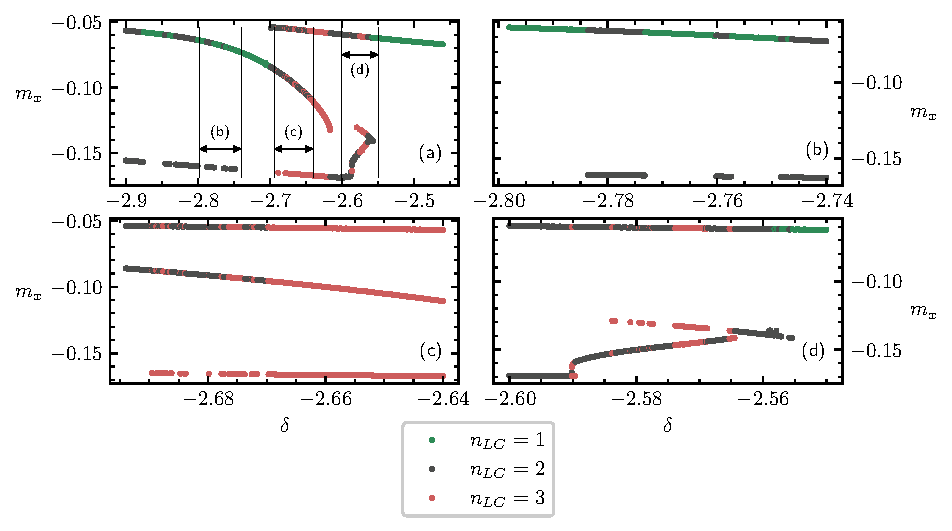
\includegraphics{pictures/multistab_line_bay.pdf}
    \caption{One dimensional cuts for the region where the multistability is incised (See \figref{fig:delta_cut_traj}). Drawn are the $m_x$-values of trajectories averaged over a period of the limit cycle. Subfigure (a) shows a wide cut through the incision. For that 1000 different values for the detuning have been considered. (b)-(d) are close up diagrams of regions marked in (a). All of them show the average of all the possible long-time states for 750 different $\delta$-values. Throughout the figure $\kappa=11.9$ and $\omega=2.39$.}
    \label{fig:delcut_bay}
\end{figure}
This section constituted the main part of the thesis. The full model with the presence of detuning has been examined with respect to stability and long-time states. I have learned in \secref{sec:stab_3D} that the system exhibits regions, in which the collective spin always ends up at stable stationary points after a certain time of convergence. These stationary solutions can be explained by synchronization, where the system adapts its oscillations to the frequency of the laser, see \secref{sec:synchronization}. \\Outside the regions of synchronization the system performs oscillations, which break free from the complete adaption to the external driving. The resulting limit cycles have been analyzed regarding to their behavior as parameters are changed, \secref{sec:multistability}. It was found that multistability arises, accompanying a change of magnitude of the mean spin value. \\Further was observed that the number of different limit cycles, that exist for a certain parameter configuration, jumps discontinuously in parameter space. Especially rich behavior is found i.a. at the borders of multistability. Repeating and highly discontinuous patterns could be observed when the detuning was altered. I will now close the thesis with a summary of its findings followed by a brief outlook to possible future investigations.


% \subsection{Basin of attraction}
% \begin{figure}[H]
%     % \vspace*{-1cm}
%     \hspace*{-1.2cm}
%     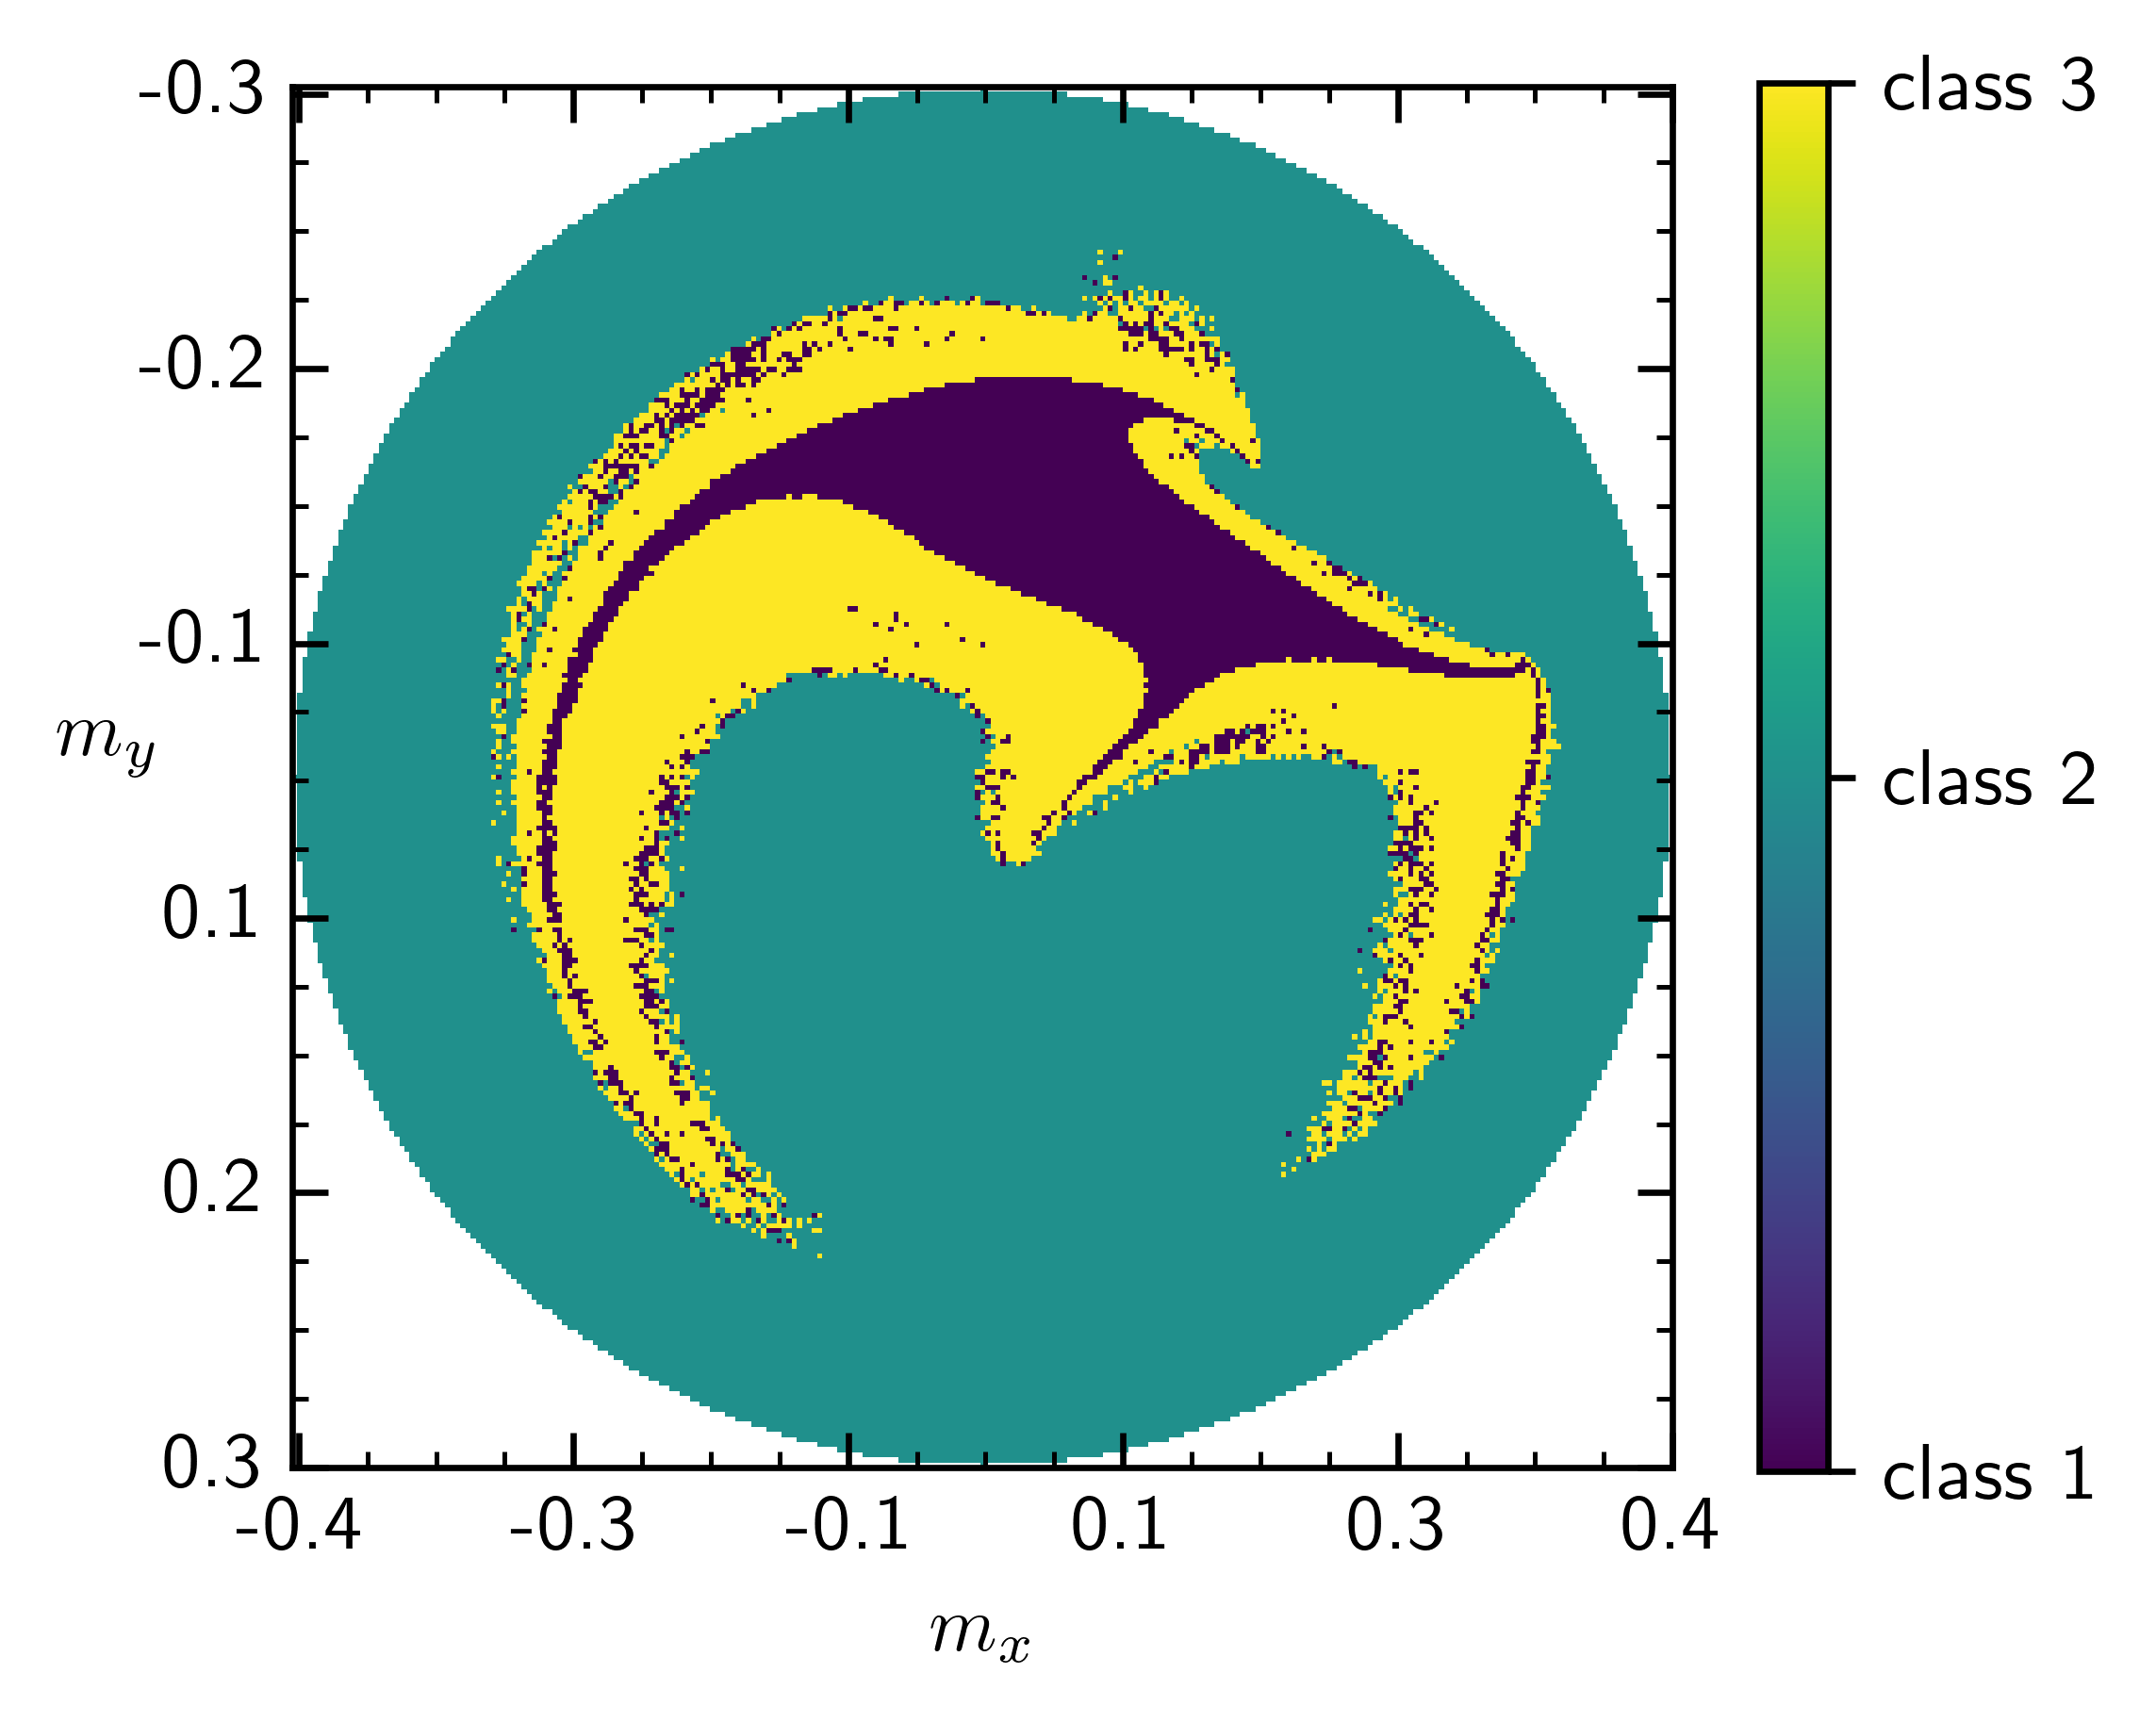
\includegraphics{pictures/phaseplot_tilted.png}
%     \caption{}
% \end{figure}
% \begin{figure}[H]
%     % \vspace*{-1cm}
%     \hspace*{-1.2cm}
%     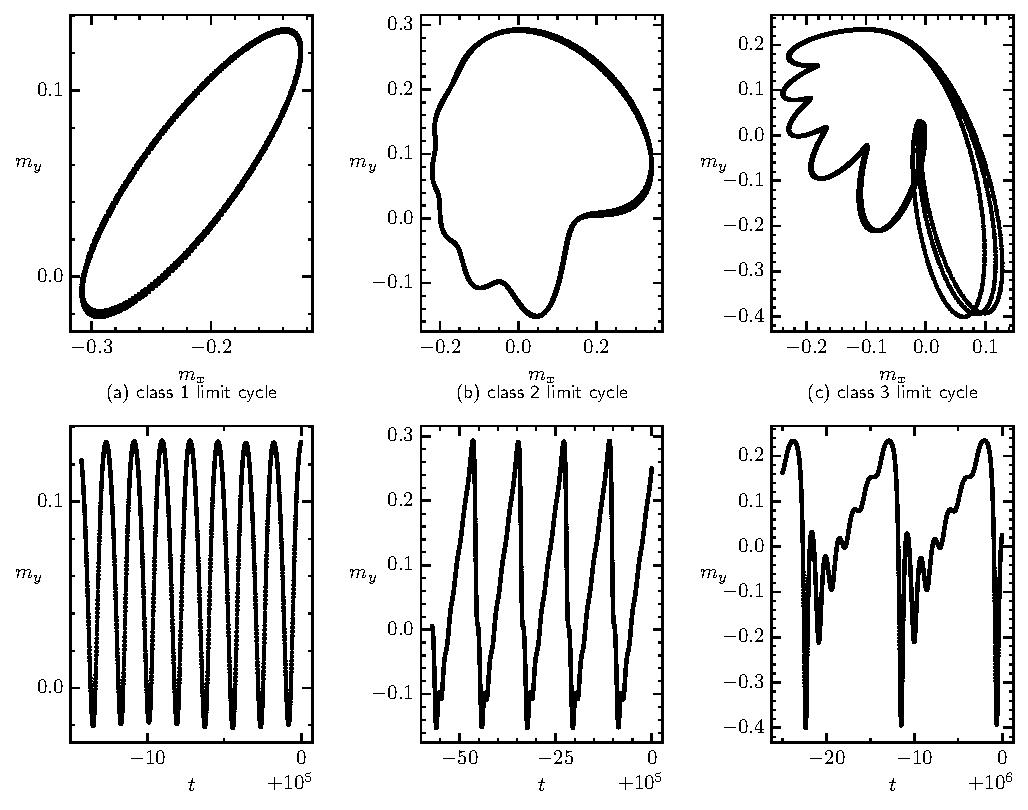
\includegraphics{pictures/classes_plot_wcut.pdf}
%     \caption{}
% \end{figure}

% \automark[section]{section}
% \lehead[\headmark]{\headmark}
% \rohead[\headmark]{\headmark}
% \lehead[Conclusion]{Conclusion}
% \rohead[Conclusion]{Conclusion}
% \automark[chapter]{chapter}
\chapter{Conclusion}
The subject of this thesis was an ensemble of non-interacting two-level atoms in the thermodynamical limit, coherently driven by a laser. The interaction of the atoms with the environment accounted for collective spontaneous emission processes, collective dephasing and a local pumping. I showed that in the absence of local pumping the system converges to a featureless fully mixed state for long times. Further it was analytically shown that the system converges to stationary non-equilibrium states, when local pumping is introduced. In the case where the laser is resonant to the atoms of the system, a stationary state is always adopted for long times. The thesis was able to demonstrate that in the presence of both, detuning and local pumping, the rise of limit cycles can be observed.% The analysis in this setup was completely performed numerically. 

One of the most intriguing learnings from this project was that the stationary states, which were present for a wide range of parameter configurations of the full model, can be explained via synchronization. In these cases the system's dynamics result from a frequency locking and follow the frequency of the laser driving. 

A time crystal phase was discovered where no stable stationary solutions to the equations of motion of the collective spin exist. Within this phase parameter configurations exist, where more than one limit cycle can be adopted for long times and hence multistability arises. This phenomenon was examined with regard to its behavior when parameters were changed. For the number of present limit cycles as well as their average values a rich dependence on the parameter configuration was observed in form of strong discontinuity and repeating patterns.\\\\
The rise of metastability is linked to a transition in the average spin values of a limit cycle. But a comprehensive understanding of this phenomenon is yet to be found. An explanation of the intriguing courses the number of present limit cycles as well as their average values take is an interesting topic for subsequent work. Also the rise of synchronization has to be analyzed in more detail, and can possibly be described through transforming the mean-field equations into a different basis, where a phase is introduced. Maybe a link between metastability and synchronization can be uncovered. Another open question is how the existence of more than one limit cycle manifests itself in the space of the collective spin. A step in this direction can be the analysis of the basin of attraction of the long-time states.

Apart from these open questions, which have been out of scope of the Bachelor project, it would also be interesting to examine the system away from the thermodynamical limit. An important task is to evaluate whether the phenomena found in this work withstand in a finite system. The permutation invariance of the atoms in the considered model can be harvested to make numerical calculations for the quantum Lindblad equations more feasible. Possible synchronization effects and time crystal phases even in the presence of dephasing can have implications for research and applications \cite{nande_integrating_2025}.

% \printbibliography


\cleardoublepage
% \lehead[]{}
% \newpage
\makedeclarationoffidelity
% \automark[section]{chapter}
% \lehead[\headmark]{\headmark}
% \rohead[\headmark]{\headmark}




% {	
% 	\thispagestyle{plain}

% 	\section*{Related publication}
% 	This thesis resulted from the research conducted in the master studies of the author. Parts of these results are already published in the following preprint:\\

% 	\begin{center}
% 		M. Cech, I. Lesanovsky, and F. Carollo, \\
% 		``Thermodynamics of quantum trajectories on a quantum computer'', \\
% 		\href{https://doi.org/10.48550/arXiv.2301.07124}{arXiv:2301.07124 (2023)},\\
% 		Submitted to \textit{Physical Review Letters} in January 2023.
% 	\end{center}
% 	\clearpage
% }
% \automark[section]{section}
% \lehead[\headmark]{\headmark}
% \rohead[\headmark]{\headmark}
\printbibliography
% \begin{appendices}
\appendix
    \chapter{Appendix for the theoretical framework}
    \section{Derivation of the equations of motion}
    \label{appendix:eqm_derv}
    
    Starting from the Lindblad master equation I will derive the different interaction's contributions to the equations of motion for the components of the collective spin. For this purpose I
    revise a few of the properties of Pauli matrices.
    \begin{align*}
        [\sigma^\alpha,\sigma^\beta]&=2i\,\varepsilon_{\alpha\beta\lambda}\,\sigma^\lambda\\
        \Rightarrow\quad[J_\alpha,J_\beta]&=i\,\varepsilon_{\alpha\beta\lambda}\,J_\lambda\\
        [\sigma^z,\sigma^\pm]&=\pm2\,\sigma^\pm\\
        \Rightarrow\quad[J_z,J_\pm]&=\pm J_\pm\\
        \sigma^x\sigma^z&=\left( \begin{array}{cc}
             0 & -1  \\
             1& 0
        \end{array}\right)=-i\,\sigma^y\\
        \sigma^y\sigma^z&=\left( \begin{array}{cc}
             0 & i  \\
             i& 0
        \end{array}\right)=i\,\sigma_x\\
        \sigma^x\sigma^y&=\left( \begin{array}{cc}
             i & 0  \\
             0 & -i
        \end{array}\right)=i\,\sigma_z\\
        \sigma^\pm\sigma^z&=-i\,\sigma^y\pm i^2\,\sigma^x=\mp\sigma^\pm\\
        \sigma^-\sigma^+&=(\sigma^x)^2+(\sigma^y)^2+i\,\sigma^x\sigma^y-i\,\sigma^y\sigma^x\\
        &=2-2\,\sigma^z\\
        \sigma^+\sigma^-&=(\sigma^x)^2+(\sigma^y)^2-i\,\sigma^x\sigma^y+i\,\sigma^y\sigma^x\\
        &=2+2\,\sigma^z\\
        [\sigma^+,\sigma^-]_-&=4\,\sigma^z
    \end{align*}
    Applying these properties one can compute the part the driving is contributing to the equations of motion.
    \begin{align*}
        \mathcal{L}_\text{drive}(J_z)&=-i\,\omega\,\braket{[J_z,J_x]}\\
        &=\omega\,\braket{J_y}\\
        \mathcal{L}_\text{drive}(J_\pm)&=-i\,\frac{\delta}{2}\,\braket{[J_\pm,J_z]}-i\,\omega\,\braket{[J_\pm,J_x]}\\
        &=-i\,\left(\mp\frac{\delta}{2}\, \braket{J_\pm} \pm \omega\, \braket{J_z}\right)
    \end{align*}
    The contributions of the remaining interaction types can be also determined using the commutation relations.
    \begin{align*}
        \mathcal{L}_\text{SpE}(J_z)&=\frac{\kappa}{N}\,\Trs{\left(J_+ J_z J_- \rho-\half\,[J_z,J_+ J_-]_+\,\rho\right)}\\
        &=\frac{\kappa}{N}\,\Trs{\left(J_z J_+ J_- - J_+ J_- -\half\,(J_z J_+ J_- + J_+ J_z J_- + J_+ J_-)\right)\,\rho}\\
        &=\frac{\kappa}{N}\,\Trs{\left(J_z J_+ J_- - J_+ J_- -\half\,(2\,J_z J_+ J_- + J_+ J_- - J_+ J_-)\right)\,\rho}\\
        &=-\frac{\kappa}{N}\,\Trs{J_+ J_- \rho}
    \end{align*}

    \begin{align*}
        \mathcal{L}_\text{SpE}(J_+)&=\frac{\kappa}{N}\,\Trs{\left(J_+ J_+ J_- \rho-\half\,[J_+,J_+ J_-]_+\,\rho\right)}\\
        &=\frac{\kappa}{N}\,\Trs{\left(J_+ J_- J_+ + 2\,J_+ J_z -\half\,(J_+ J_- J_+ + J_+ J_+ J_-)\right)\,\rho}\\ &=\frac{\kappa}{N}\,\Trs{\left(J_+ J_- J_+ + 2\,J_+ J_z -\half\,(2\,J_+ J_- J_+ + 2 J_+ J_z)\right)\,\rho}\\\\
        &=\frac{\kappa}{N}\,\Trs{J_+ J_z \rho}\\\\
        \mathcal{L}_\text{SpE}(J_-)&=\frac{\kappa}{N}\,\Trs{\left(J_+ J_- J_- \rho-\half\,[J_-,J_+ J_-]_+\,\rho\right)}\\
        &=\frac{\kappa}{N}\,\Trs{\left(J_- J_+ J_- + 2\,J_z J_- -\half\,(J_- J_+ J_- + J_+ J_- J_-)\right)\,\rho}\\ 
        &=\frac{\kappa}{N}\,\Trs{J_z J_- \rho}
    \end{align*}
    \begin{align*}
        \mathcal{L}_\text{Dp}(J_z)&=0\\
        \mathcal{L}_\text{Dp}(J_\pm)&=\gamma\,\Trs{\left(J_z J_\pm J_z \rho-\half\,[J_\pm,J_z^2]_+\,\rho\right)}\\
        &=\gamma\,\Trs{\left(J_\pm J_z^2\rho \pm J_\pm J_z \rho-\half\,(J_\pm J_z^2 + J_z J_\pm J_z \pm J_z J_\pm)\,\rho\right)}\\
        &=\gamma\,\Trs{\left(J_\pm J_z^2\rho \pm J_\pm J_z \rho-\half\,(2\,J_\pm J_z^2  \pm J_z J_\pm \pm J_\pm J_z)\,\rho\right)}\\
        &=\pm\half\, \gamma\,\Trs{[J_\pm,J_z]\,\rho}\\
        &=-\half\,\gamma\,\Trs{J_\pm\rho}
    \end{align*}
    \begin{align*}
        \mathcal{L}_\text{pump}(J_z)&=\frac{\Gamma}{8}\,\sum_{j,k=1}^N \Trs{\left( \sigma_j^- \sigma_k^z \sigma_j^+ -\half\,[\sigma_k^z,\sigma_j^-\sigma_j^+]_+   \right)\,\rho}\\
        &=\frac{\Gamma}{8}\,\sum_{j,k=1}^N \Trs{\left( \sigma_j^- \sigma_k^z \sigma_j^+ -\half\,[\sigma_k^z\sigma_j^-\sigma_j^++\sigma_j^-\sigma_j^+\sigma_k^z]   \right)\,\rho}\\
        &=\frac{\Gamma}{8}\,\sum_{j,k=1}^N \Trs{\left( \sigma_j^- \sigma_k^z \sigma_j^+ -\half\,[2\,\sigma_j^-\sigma_k^z\sigma_j^+  -2\, \sigma_j^-\sigma_j^+\delta_{jk}-2\, \sigma_j^-\sigma_j^+\delta_{jk}]   \right)\,\rho}\\
        &=\frac{\Gamma}{8}\,\sum_{k=1}^N \Trs{2\, \sigma_k^-\sigma_k^+  \,\rho}\\
        &=\frac{\Gamma}{4}\,\sum_{k=1}^N \Trs{ (2-2\,\sigma_k^z)  \,\rho}\\
        &=\half\,N\,\Gamma-\Gamma\,\braket{J_z}
    \end{align*}
    \begin{align*}
        \mathcal{L}_\text{pump}(J_-)&=\frac{\Gamma}{4}\,\sum_{j,k=1}^N \Trs{\left( \sigma_j^- \sigma_k^- \sigma_j^+ -\half\,[\sigma_k^-,\sigma_j^-\sigma_j^+]_+   \right)\,\rho}\\
        &=\frac{\Gamma}{4}\,\sum_{k=1}^N \Trs{\left( \sigma_k^- \sigma_k^- \sigma_k^+ -\half\,[\sigma_k^-\sigma_k^-\sigma_k^++\sigma_k^-\sigma_k^+\sigma_k^-]   \right)\,\rho}\\
        &=-\frac{\Gamma}{2}\,\sum_{k=1}^N\Trs{\sigma_k^-\sigma_k^z\rho}\\
        &=-\frac{\Gamma}{2}\,\sum_{k=1}^N\Trs{\sigma_k^-\rho}\\\\
        \mathcal{L}_\text{pump}(J_+)&=\frac{\Gamma}{4}\,\sum_{j,k=1}^N \Trs{\left( \sigma_j^- \sigma_k^+ \sigma_j^+ -\half\,[\sigma_k^+,\sigma_j^-\sigma_j^+]_+   \right)\,\rho}\\
        &=-\frac{\Gamma}{2}\,\sum_{k=1}^N\Trs{\sigma_k^z\sigma_k^+\rho}\\
        &=-\frac{\Gamma}{2}\,\sum_{k=1}^N\Trs{\sigma_k^+\rho}
    \end{align*}
    
    \chapter{Appendix for zero detuning}
    \section{Decay without pumping}
    \label{appendix:msq_calc}
    In this paragraph I want to discuss, why in the absence of pumping the system always decays to fully mixed state. But first I want to derive a statement, which can be applied to certain driven-dissipative models, as they often encounter a similar form of the derivative  for the squared of the total spin. For this purpose assume that the coupled set of $N$ ordinary differential equations has the solution $\vec{F}:\,\mathbb{R}\rightarrow\mathbb{R}^N$. Define from that the function squared $F^2:\,\mathbb{R}\rightarrow\mathbb{R}:\,t\mapsto\sum_{i=1}^NF_i^2(t)$. The statement is now, that if one is able to write the derivative of the squared function in the following way
    \begin{align*}
        \half\,\dt F^2(t)&=\vec{F}^t(t)\,A\,\vec{F}(t)
    \end{align*}
    with a Matrix $A$, which is positive ore negative definite, then the only stationary solution to the system of ODE is $\vec{F}\equiv\vec{0}$. Further limit cycles can not exist. \\
    \textit{Proof}: The function $\vec{F}$, can be mapped via N-dimensional spherical coordinates into a different set of functions $f(t)$, $\varphi_j(t)$ $j\in\{1,\dots,N-1\}$, with $f$ the modulus of $F$, and $\varphi_j$ the angles. This is true for all solutions $\vec{F}\neq\vec{0}$. In the following I neglect this special case, as this is in the most cases anyway a stationary point and I am not interest in this part of the spin space. With the notation.
    \begin{align*}
        \vec{F}(t)&=f(t)\,\hat{r}(t)
    \end{align*}
    One can rewrite the differential equation for the squared function to
    \begin{align*}
        \half\,\dt F^2(t)=\half\,\dt f^2(t)=f(t)\,\dt f(t)&=f^2(t)\,\hat{r}^t\,A\,\hat{r}\\
        \Rightarrow\quad\dt f(t) = f(t)\,\hat{r}^t\,A\,\hat{r}
    \end{align*}
    Assuming that A is positive or negative definite one can use the property that $|\hat{r}(t)|=1\,\forall t$, in order to follow, that there exists an $\varepsilon>0$ so that
    \begin{align*}
        \lambda(t)\vcentcolon=\left| \hat{r}^t(t)\,A\,\hat{r}(t) \right| > \varepsilon
    \end{align*}
    For all $t$ and all functions $\{\varphi_j(t)\}$. \textit{Proof}: if this does not hold, there will have to be a sequence $(t_n)$ with $\lambda(t_n)\rightarrow0$. As the surface of an N-dimensional sphere is a compact set, this sequence would have to converge on the survace of the sphere, which would infer $\exists \hat{r}\neq0$ with 
    \begin{align*}
        \hat{r}^t(t)\,A\,\hat{r}(t)=0
    \end{align*}
    in contradiction to the definiteness of $A$. So depending on, whether $A$ is positive or negative definite, one can write
    \begin{align*}
        \dt f(t) >& \varepsilon\,f(t)\\
        \Rightarrow\quad f(t) >& c\,e^{\varepsilon\,t}\\
        \text{or}\quad \dt f(t) <& -\varepsilon\,f(t)\\
        \Rightarrow\quad f(t) <& c\,e^{-\varepsilon\,t}\\
    \end{align*}
    for suitable choice of $c$ (can be shown with mean value theorem). This implies, that there can't be a stationary solution of the set of ODE. The last statement holds, because for $t\rightarrow\infty$ either $f$ goes to zero, which would imply that all $F_i$ go to zero or $f$ grows boundlessly, which implies that, independent of the starting conditions, there exists a $F_i$, that grows boundlessly, which forbids the properties of a stationary state including limit cycles.\\\\Now in the case of the equations of motion in this work, the matrix $A$ is negative semi-definite in the absence of pumping. Nevertheless one can infer from the form of $A$ and the equations of motion that limit cycles can not exist and the only stationary state is $\vec{m}=0$. This can be seen by the following consideration. First revise the equations of motion for $\Gamma=0$
    \begin{align*}
        \dt m_x &= -\frac{\delta}{2}\,m_y-\half\,\gamma\,m_x+\kappa\,m_x m_z\\
        \dt m_y &= \frac{\delta}{2}\,m_x-\omega\,m_z-\half\,\gamma\,m_y+\kappa\,m_y m_z\\
        \dt m_z &= \omega\,m_y - \kappa\,(m_x^2+m_y^2)
    \end{align*}
    Accordingly the modulus of the total spin obeys the dynamics
    \begin{align*}
        \half\dt |m|^2=&-\half\,\hat{m}^t\,\left( \begin{array}{ccc}
            \gamma & 0&0  \\
            0& \gamma & 0\\
            0&0&0
       \end{array}\right)\,\hat{m}
    \end{align*}
    where $\hat{m}=\vec{m}/|m|$. In order for a vector to be a stationary solution, the derivatives of all spin components as well as the derivative of the total spin have to vanish. The latter condition implies $m_x=m_y=0$ and the combination with $\text{d}m_y/\text{d}t=0$ also demands $m_z=0$. Hence the fully mixed state is the only possible stationary point. Limit cycles can not exist either. This is found true by first noticing, that, because of the negative semi-definiteness of $A$, the total spin cannot grow. Thus in order for the system to have stable oscillations the total spin has to be constant, which implies that again $m_x=m_y=0$ has to hold. But this results in $m_z$ being constant. Hence no stable oscillations can occur.
    \newpage




    \section{Modulus of the fixed points in the case $\delta=0$}
    \label{appendix:mod_of_fixp}
    Here it is shown that all stationary solutions of the equations of motion without detuning are in the physically allowed set of values, i.e. $|m|\leq1/2$.
    The idea of the following analysis is to show first that $|m|$ is monoton in the parameters and then look at the maximum values. I begin by getting an expression for the modulus of the total spin.
    
    \begin{align*}
        m_z&=\half-\frac{1}{\Gamma}\,\left( \kappa\,(m_x^2+m_y^2)-\omega m_y  \right)\\
        &=\half-\frac{\kappa}{\Gamma}\,\left( m_y^2-\frac{\omega}{\kappa}\, m_y  \right)\\
        \Rightarrow\quad |m|^2&=\left( \half-\frac{\kappa}{\Gamma}\,\left( m_y^2-\frac{\omega}{\kappa}\, m_y  \right) \right)^2+m_y^2\\
        &=\left( \half-\frac{\omega^2}{\Gamma\kappa}\,\left( {y}^2- {y} \right) \right)^2+\frac{\omega^2}{\kappa^2}\,{y}^2\\
        &=\left( \half-\frac{\Omega^2}{K}\,\left( {y}^2- {y} \right) \right)^2+\frac{\Gamma}{\Gamma+\gamma}\,\frac{\Omega^2}{K^2}\,{y}^2\\
        \leq&\left( \half-\frac{\Omega^2}{K}\,\left( {y}^2- {y} \right) \right)^2+\frac{\Omega^2}{K^2}\,{y}^2\\
        &=\vcentcolon m^*
    \end{align*}
    The last definition allows to continue the analysis with only two parameters $K$, $\Omega$. The real magnetic modulus squared is always smaller than $m^*$. In order to take into account the interdependence of $y$ and the parameters through the determining equation for $y$, I have to express them through each other. 
    \begin{align*}
        0&=F(y)=-\frac{K}{2\Omega^2}-\left( \frac{1-K}{2\Omega^2} +1\right)\,{y}-{y}^3+2\,{y}^2\\
        \Rightarrow\quad \frac{K}{2\Omega^2}\,({y}-1)&=(1+\frac{1}{2\Omega^2})\,{y}+{y}^3-2\,{y}^2\\
        \frac{\Omega^2}{K}&=\frac{{y}-1}{2\,\left(  (1+\frac{1}{2\Omega^2})\,{y}+{y}^3-2\,{y}^2\right)}
    \end{align*}
    This equation looks at first strange, because $K/2\Omega^2$ could be negative for $0<{y}<1$. But as has been already seen in \figref{fig:sign_lam1}, this space is free of fixed points. For the computation of the derivative of $m^*$, the following is useful. 
    \begin{align*}
        \frac{\text{d}}{\text{d}{y}}\,\frac{\Omega^2}{K}&=\frac{1}{2\,\left(  (1+\frac{1}{2\Omega^2})\,{y}+{y}^3-2\,{y}^2\right)}-\frac{2\,({y}-1)\,(1+\frac{1}{2\Omega^2}+3\,{y}^2-4\,{y})}{4\,\left(  (1+\frac{1}{2\Omega^2})\,{y}+{y}^3-2\,{y}^2\right)^2}\\\\
        &=\frac{1+\frac{1}{2\Omega^2}-4\,{y}+5\,{y}^2-2\,{y}^3}{2\,\left(  (1+\frac{1}{2\Omega^2})\,{y}+{y}^3-2\,{y}^2\right)^2}
    \end{align*}
    The derivative of $m^*$ is calculated via
    \begin{align*}
        \frac{\partial m^*}{\partial{y}}&=-2\,\left(\frac{\Omega^2}{K}\,(2{y}-1)+\left(\frac{\text{d}}{\text{d}{y}}\,\frac{\Omega^2}{K}\right)\,({y}^2-{y})\right)\,\left( \half-\frac{\Omega^2}{K}\,\left( {y}^2- {y} \right) \right)+2\,\frac{\Omega^2}{K^2}\,{y}+2\,\left(\frac{\text{d}}{\text{d}{y}}\,\frac{\Omega^2}{K}\right)\,\frac{\Omega^2}{K}\,\frac{1}{\Omega^2}\,{y}^2\\\\
        &=4\,(\frac{\Omega^2}{K})^2\,{y}^3-\left(2\,(\frac{\Omega^2}{K})^2+4\,(\frac{\Omega^2}{K})^2\right)\,{y}^2+\left( 2\,(\frac{\Omega^2}{K})^2+2\,\frac{\Omega^2}{K^2}-2\,\frac{\Omega^2}{K} \right)\,{y}+\frac{\Omega^2}{K}\\\\
        &+2\,\dkw\,\kw\,{y}^4-4\,\dkw\,\kw\,{y}^3\\\\
        &-\left(\dkw-2\,\dkw\,\kw-2\,\dkw\,\kw\,\frac{1}{\Omega^2}\right)\,{y}^2+\dkw\,{y}\\\\
        &=\frac{\Omega^2}{K}\,\left[  4\,\frac{\Omega^2}{K}\,{y}^3-6\,\frac{\Omega^2}{K}\,{y}^2+\left( 2\,\frac{\Omega^2}{K}+2\,\frac{\Omega^2}{K}\,\frac{1}{\Omega^2}-2 \right)\,{y}+1 \right]\\\\
        &+\dkw\,\left[2\,\kw\,{y}^4-4\,\kw\,{y}^3-\left(1-2\,\kw-2\,\kw\,\frac{1}{\Omega^2}\right)\,{y}^2+{y}\right]\\\\
        &=\vcentcolon \frac{\partial \alpha}{\partial{y}}+\dkw\,\frac{\partial \beta}{\partial{y}}
    \end{align*}
    
    Plugging the former expression into the equation for the derivative of $m^*$ yields
    \begin{align*}
        \frac{2\,\left[(1+\frac{1}{2\Omega^2})\,{y}+{y}^3-2\,{y}^2\right]^2}{{y}-1}\,\frac{\partial \alpha}{\partial{y}}&=2\,({y}-1)\,{y}^3-3\,({y}-1)\,{y}^2\\
        &+\left( {y}-1+({y}-1)\,\frac{1}{\Omega^2}-2\,\left((1+\frac{1}{2\Omega^2})\,{y}+{y}^3-2\,{y}^2\right) \right)\,{y}\\
        &+(1+\frac{1}{2\Omega^2})\,{y}+{y}^3-2\,{y}^2 \\\\
        &=3\,{y}^2+\left( -(1+\frac{1}{\Omega^2})-{y}\right)\,{y}+(1+\frac{1}{2\Omega^2})\,{y}-2\,{y}^2\\
        &=-\frac{1}{2\Omega^2}\,{y}\\\\
        \Rightarrow\quad\frac{\partial \alpha}{\partial{y}}&=-\frac{{y}-1}{2\,\left[(1+\frac{1}{2\Omega^2})\,{y}+{y}^3-2\,{y}^2\right]^2}\,\frac{1}{2\Omega^2}\,{y}
    \end{align*}
    Doing the same for the $\beta$-expression, one finds
    \begin{align*}
        \left[(1+\frac{1}{2\Omega^2})\,{y}+{y}^3-2\,{y}^2\right]\,\frac{\partial \beta}{\partial{y}}&=({y}-1)\,{y}^4-2\,({y}-1)\,{y}^3-\left( (1+\frac{1}{2\Omega^2})\,{y}+{y}^3-2\,{y}^2-{y}+1-({y}-1)\,\frac{1}{\Omega^2} \right)\,{y}^2\\
        &+((1+\frac{1}{2\Omega^2})\,{y}+{y}^3-2\,{y}^2)\,{y}\\
        &=-\left( 1+\frac{1}{\Omega^2}-\frac{1}{2\Omega^2}\,{y}  \right)\,{y}^2+(1+\frac{1}{2\Omega^2})\,{y}^2\\
        &=\frac{1}{2\Omega^2}\,({y}^3-{y}^2)=\frac{1}{2\Omega^2}\,{y}^2\,({y}-1)
    \end{align*}
    After joining all terms, one finds
    \begin{align*}
        \frac{\partial \alpha}{\partial{y}}+\dkw\,\frac{\partial \beta}{\partial{y}}&=-\frac{\frac{1}{2\Omega^2}\,({y}-1)}{2\,\left[(1+\frac{1}{2\Omega^2})\,{y}+{y}^3-2\,{y}^2\right]^3}\,\left( {y}\,((1+\frac{1}{2\Omega^2})\,{y}+{y}^3-2\,{y}^2) -{y}^2\,(1+\frac{1}{2\Omega^2}-4\,{y}+5\,{y}^2-2\,{y}^3)\right)\\
        &=-\frac{\frac{1}{2\Omega^2}\,({y}-1)}{2\,\left[(1+\frac{1}{2\Omega^2})\,{y}+{y}^3-2\,{y}^2\right]^3}\,\left( 2\,{y}^5-4\,{y}^4+2\,{y}^3 \right)\\
        &=-\frac{\frac{1}{2\Omega^2}\,({y}-1)}{2\,\left[(1+\frac{1}{2\Omega^2})+{y}^2-2\,{y}\right]^3}\,\left( 2\,{y}^2-4\,{y}+2 \right)
    \end{align*}
    The quadratic polynomial in the denominater is always positive as it is positive for $y=0$ and has no roots.
    \begin{align*}
        0&=(1+\frac{1}{2\Omega^2})+{y}^2-2\,{y}\\
        y_\text{roots}&=\half\,(2\pm\sqrt{4-4\,(1+\,\frac{1}{2\Omega^2})})\\
        &=2\pm\sqrt{-\frac{1}{2\Omega^2}}
    \end{align*}
    By rewriting $2\,y^2-4\,y+2=2\,(y-1)^2$ the derivative of $m^*$ can be written as
    \begin{align*}
        \frac{\partial m^*}{\partial{y}}&=-\frac{\frac{1}{2\Omega^2}\,({y}-1)^3}{\left[(1+\frac{1}{2\Omega^2})+{y}^2-2\,{y}\right]^3}
    \end{align*}
    It can be inferred, that $\partial_{{y}}\,m^*>0$ for ${y}<1$ and $\partial_{{y}}\,m^*<0$ for ${y}>1$. As mentioned before these are the only two areas in which ${y}$ can fall. For $y$ smaller than zero $m^*$ takes it's maximum for ${y}\rightarrow0$ and for the area ${y}>1$ $m^*$ takes it's maximum for ${y}\rightarrow1$. Looking again at the form of $|m|^2$ 
    \begin{align*}
        |m|^2\leq m^*=\left( \half-\frac{\Omega^2}{K}\,\left( {y}^2- {y} \right) \right)^2+\frac{\Omega^2}{K^2}\,{y}^2
    \end{align*}
    The limit of ${y}\rightarrow1$ can only be achieved in the limit $\Omega\rightarrow\infty$, while% i.e. $\Gamma/\omega^2\rightarrow0$, while
    \begin{align*}
        \text{constant}=\frac{K}{\Omega^2}=\frac{\kappa\Gamma}{\omega^2}
    \end{align*}
    This means in particular, that also $K\rightarrow\infty$ and therefore $K^2/\Omega^2\rightarrow\infty$. But this fixes $|m|$ to $1/2$. \\\\
    The case $y\rightarrow0$ requires $K/2\Omega^2\rightarrow0$. With the use of the theorem over implicit functions \cite{deitmar_analysis_2021}, one can calculate the the derivative of $y$ with respect to $K/2\Omega^2=\vcentcolon\tau$, as follows
    \begin{align*}
        \frac{\diff y}{\diff\tau}\Big|_{y=0,\,\tau=0}=-\frac{\partial F}{\partial\tau}\Big|_{y=0,\,\tau=0}\,\left(\frac{\partial F}{\partial y}\Big|_{y=0,\,\tau=0}\right)^{-1}=\frac{1}{\frac{1}{2\,\Omega^2}+1}
    \end{align*}
    $F$ denotes the determining function for $y$. 
    \begin{align*}
        F(y)=-\frac{K}{2\Omega^2}-\left( \frac{1-K}{2\Omega^2} +1\right)\,{y}-{y}^3+2\,{y}^2
    \end{align*}
    With this result, one is able to compute the fractions $y/\tau$ in the limit $\tau\rightarrow\infty$. One proceeds by
    \begin{align*}
        m^*&=\left( \half- \half\,\frac{1}{\tau}\,(y^2-y) \right)^2+\frac{1}{4\Omega^2}\,\frac{y^2}{\tau^2}\\
        &=\frac{1}{4}\,\left( 1- \frac{1}{\frac{1}{2\Omega^2}+1}\right)^2+\frac{1}{4\Omega^2}\,\frac{1}{\left(\frac{1}{2\Omega^2}+1\right)^2}\\
        &=\left(\frac{1}{4}+\Omega^2\right)\,\frac{1}{\left(\frac{1}{2\Omega^2}+1\right)^2}\\
        &=\frac{1}{4}\,\frac{1+4\,\Omega^2}{1+4\,\Omega^2+4\,\Omega^4}\leq\frac{1}{4}
    \end{align*}
    Thus also in this case the physical boundary of $|m|$ is not violated. Drawing the numerically found fixed points in the $yz$-plane, confirms these findings. All stationary points of the mean field equations of motion lie in the physical space.
    \begin{figure}[H]
        \hspace*{-0.4cm}
        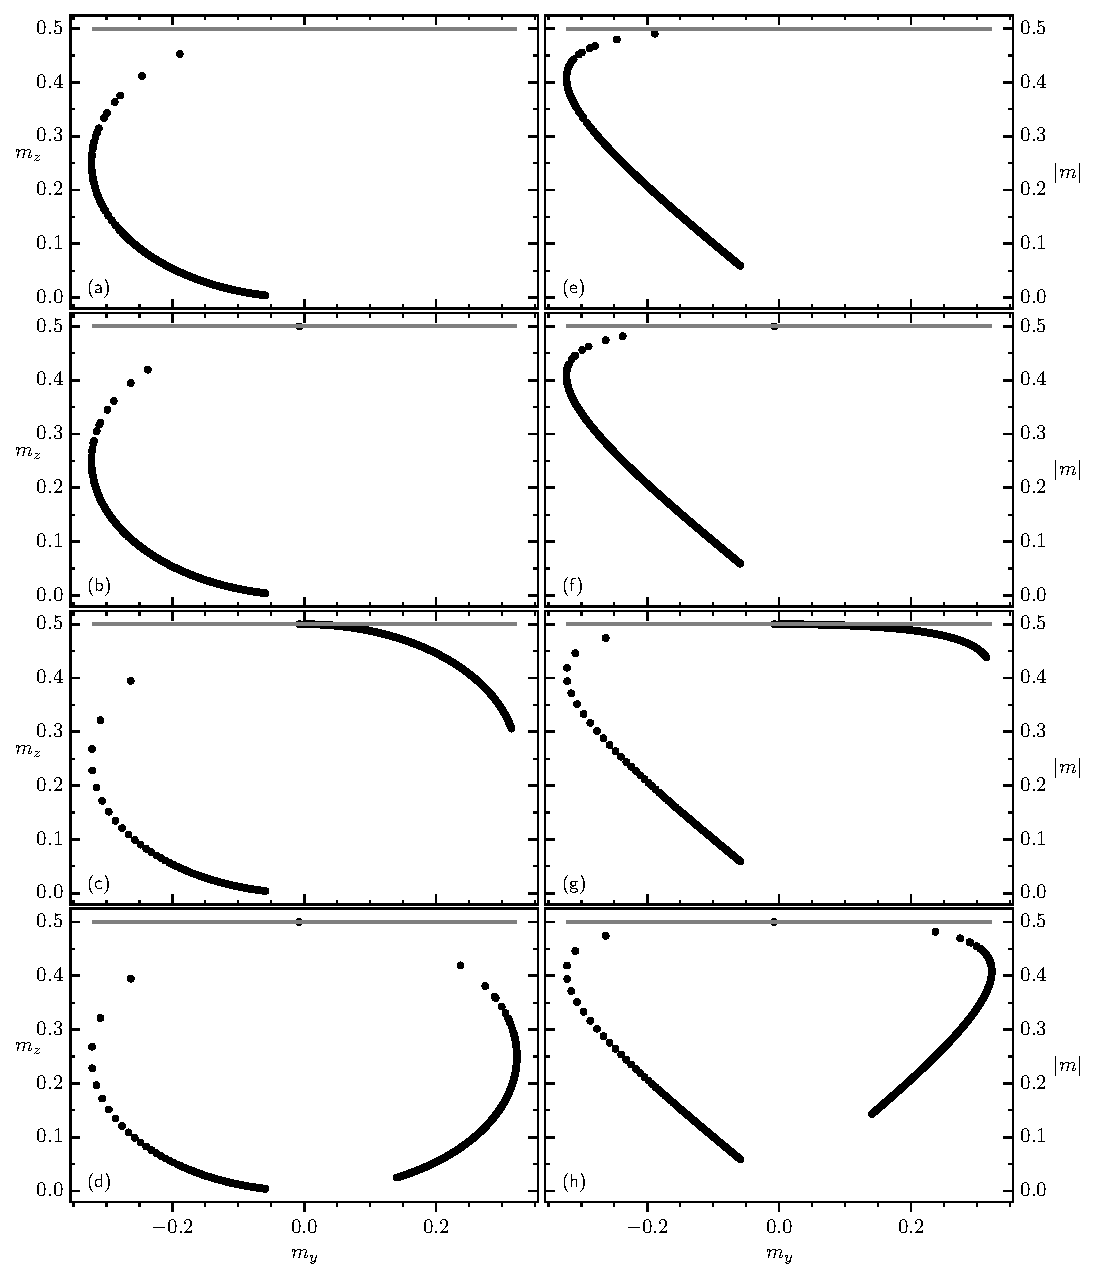
\includegraphics{pictures/fixp_boundaries.pdf}
        \caption{This graphic showes the range of $m_y$, $m_z$, $|m|$ for a parameter grid of $1.2\leq\kappa\leq24$ and $3\cdot10^{-7}\leq\omega\leq7$, $\Gamma=1$ $\gamma=0.2$. In the left column (a-d) the fixed points are shown in the $y-z$-plane, whereas in the right column (e-h) the modulus of the total angular momentum is depectid in dependence of $m_y$ for the different parameter values. The first row shows the fixed point in the parameter regime, where there is only one fixed point present. From the 2. row downwards the fixed points in the area of three stationary solutions are show in the order smallest, middle and largest $m_y$-value.}
    \end{figure}
    
    
    
    \section{Linearization eigenvalues for the unstable fixed points in the case $\delta=0$}
    \label{appendix:eig_del0}
    In this section of the appendix the eigenvalues of the linearization matrix for fixed points with middle and largest $y$-value are depicted. They show again their instability.
    \begin{figure}[H]
        \centering
        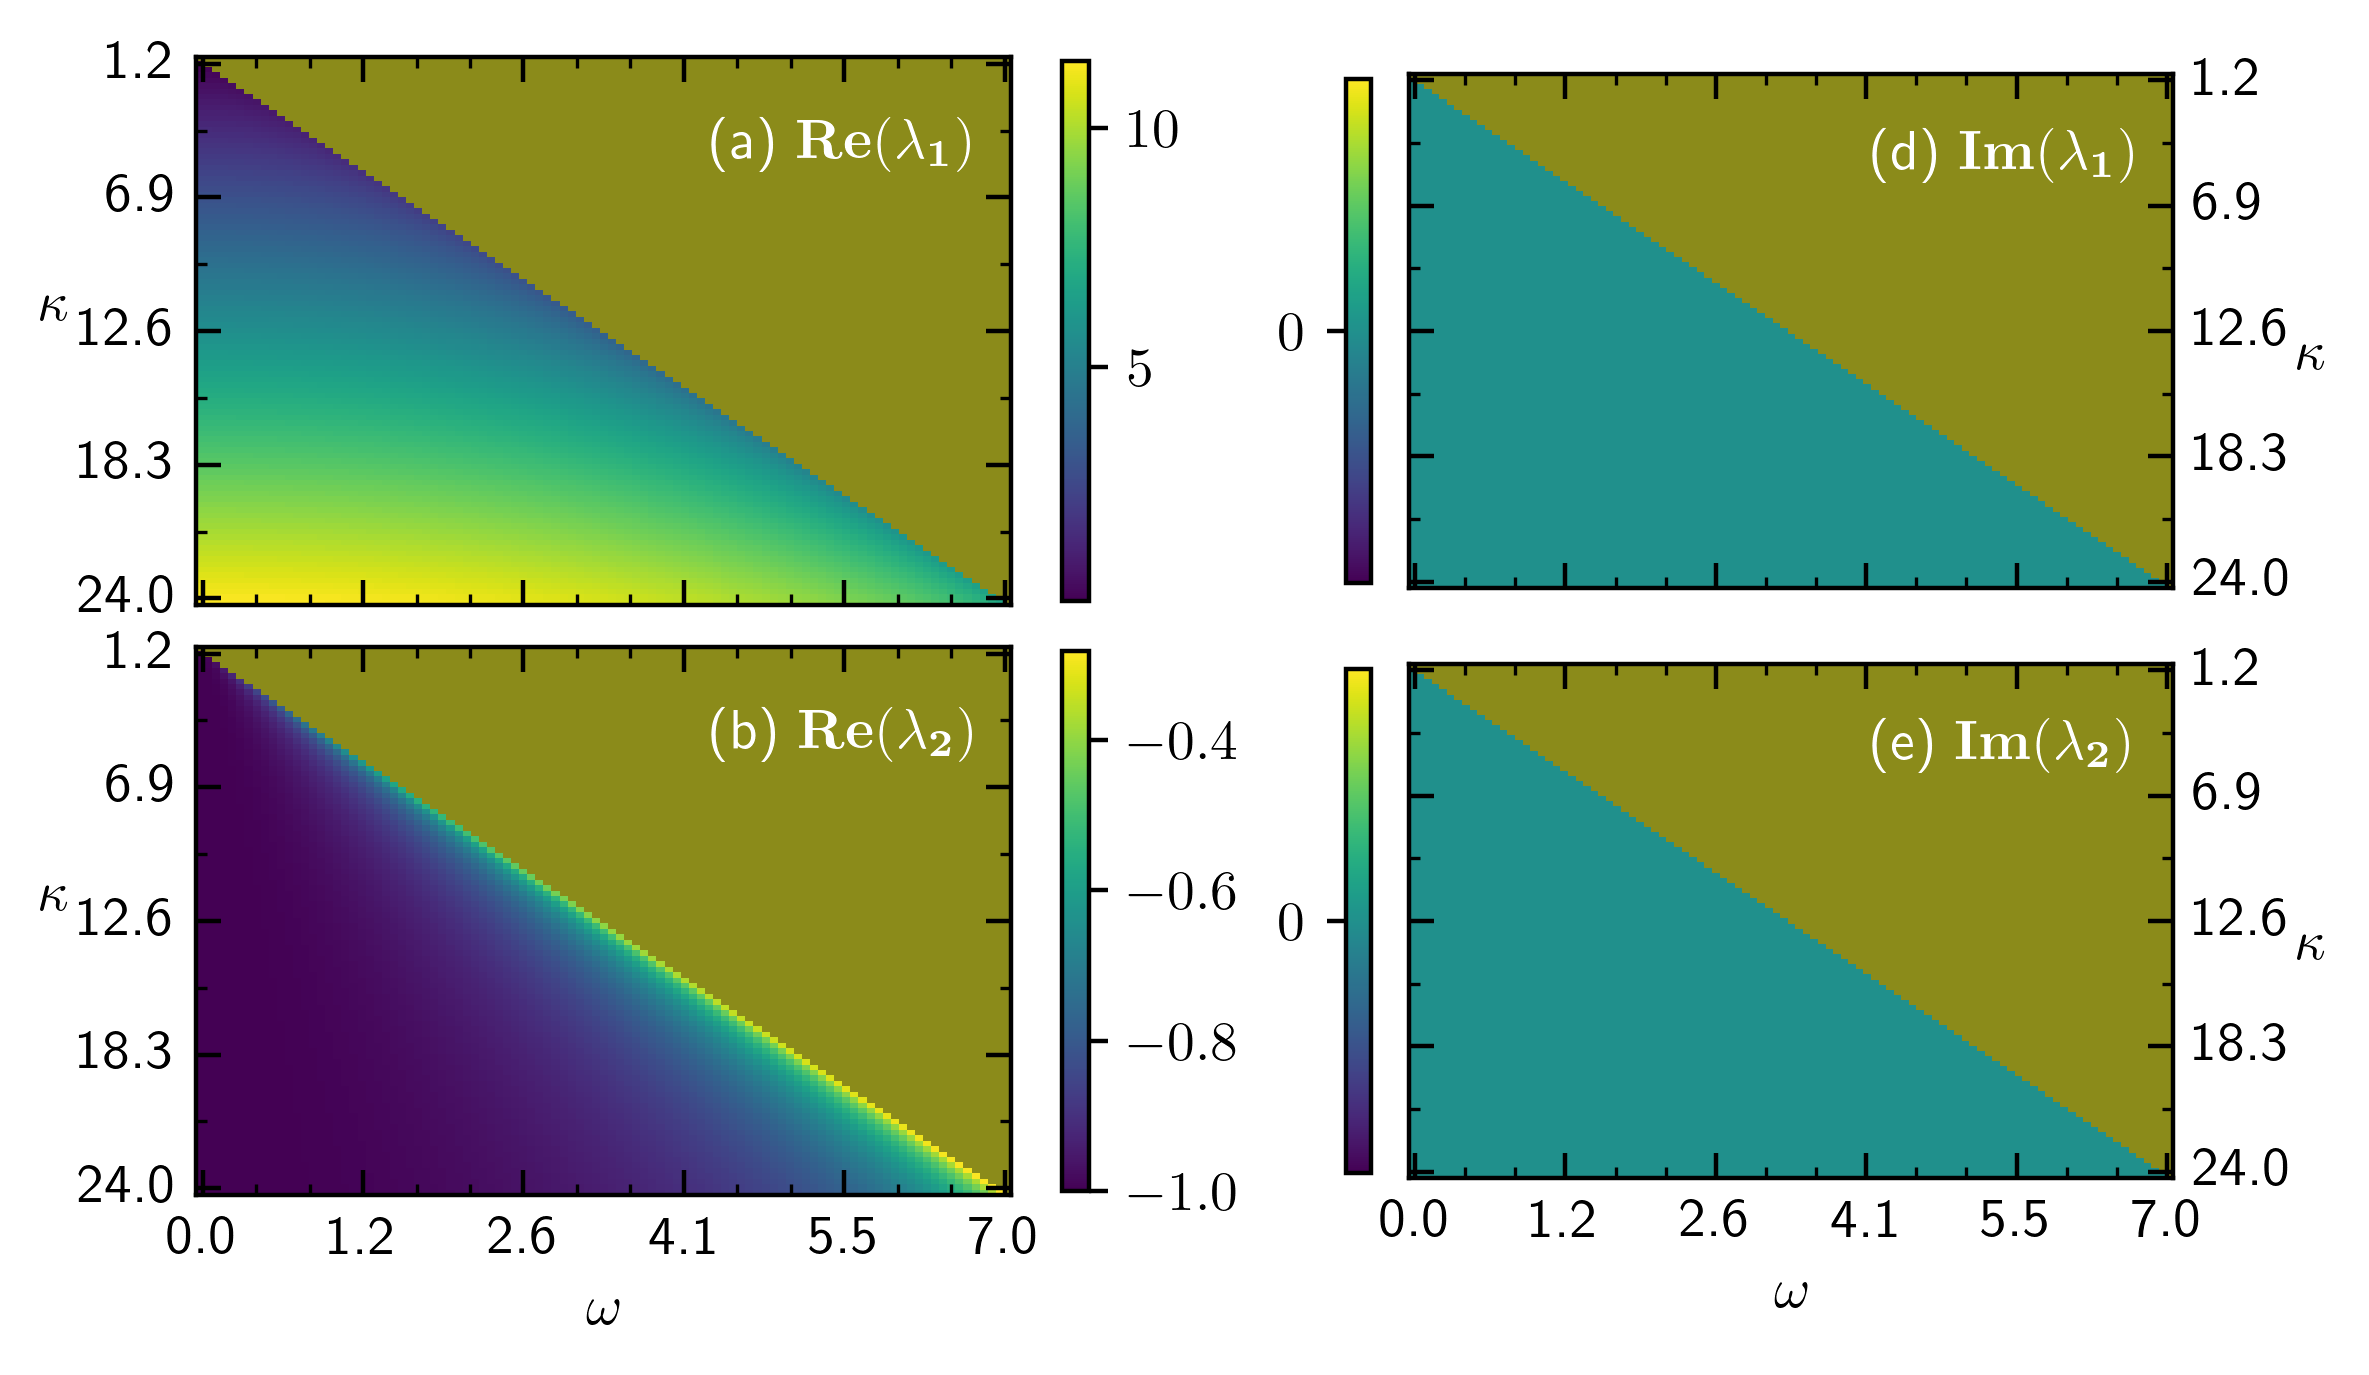
\includegraphics{pictures/lam_anal_m1.png}
        \caption{Real and imaginary part of the two of the eigenvalues of the linearization for the middle-$y$ stationary solution.
        }
    \end{figure}
    
    \begin{figure}[H]
        \centering
        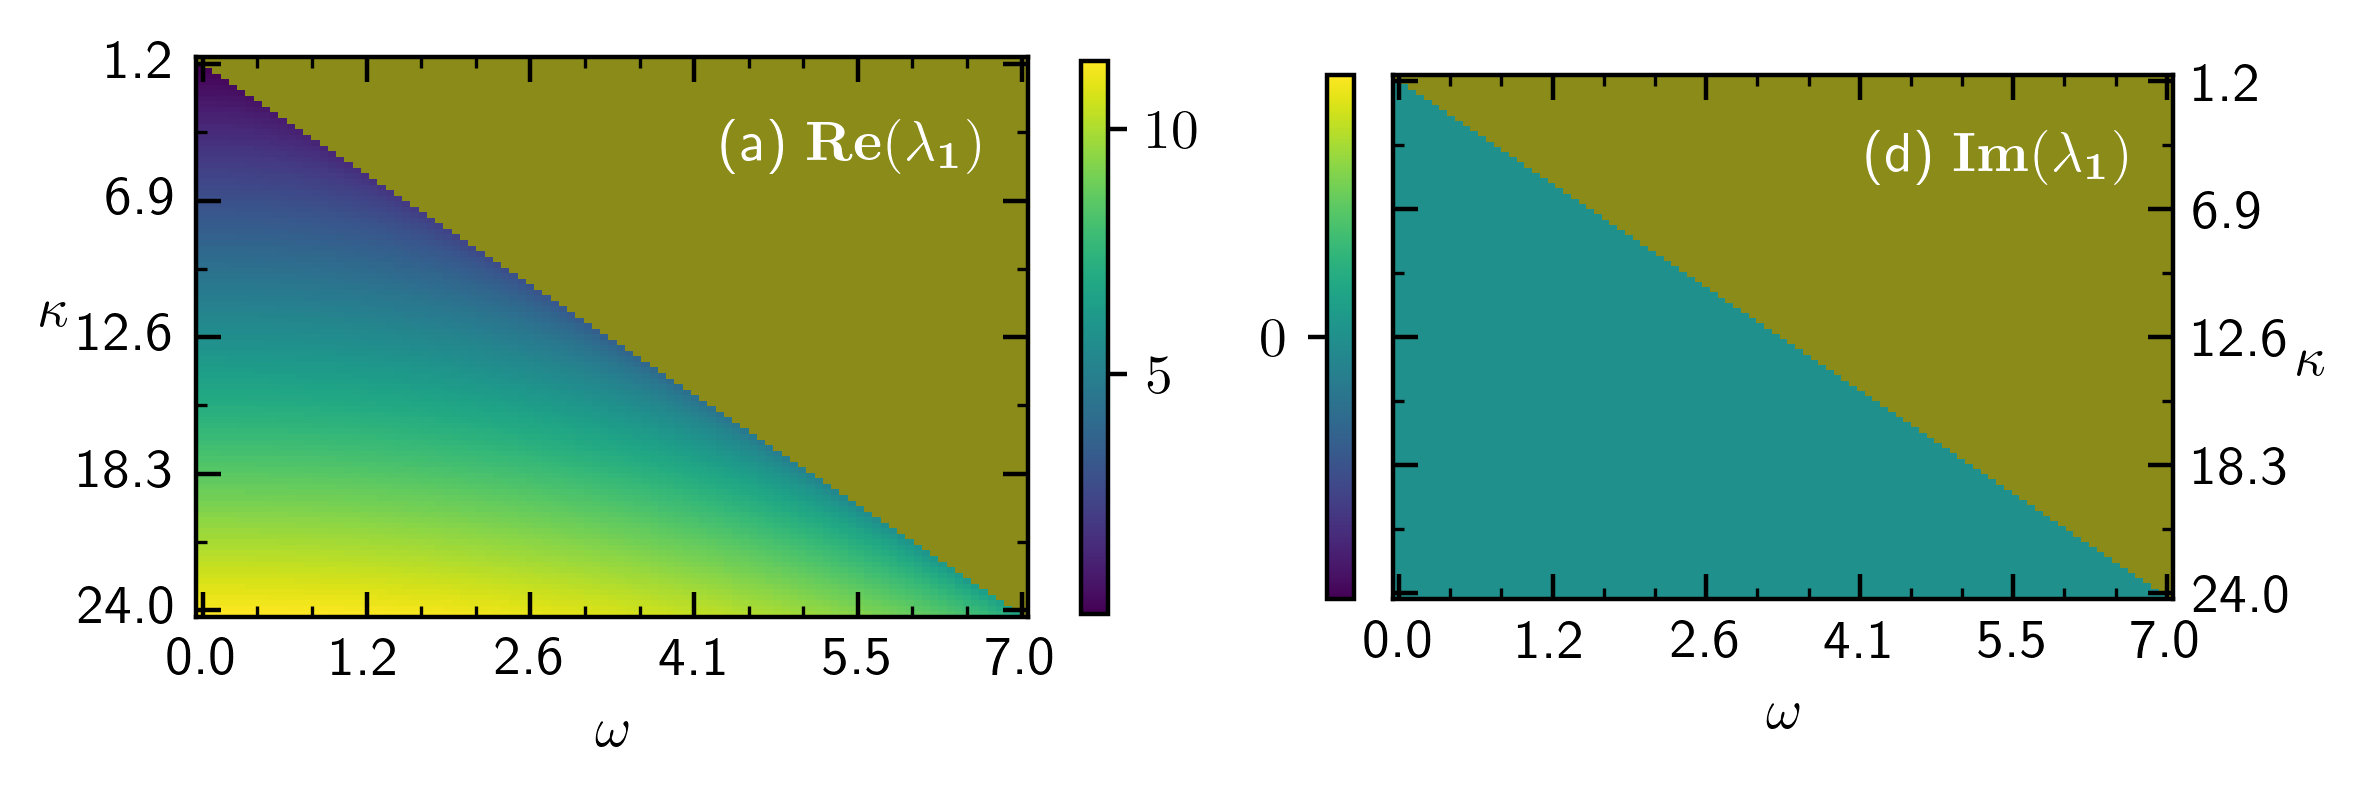
\includegraphics{pictures/lam_anal_m2.png}
        \caption{The remaining eigenvalue of the linearization for the the middle-$y$ stationary solution.
        }
    \end{figure}
    \begin{figure}[H]
        \centering
        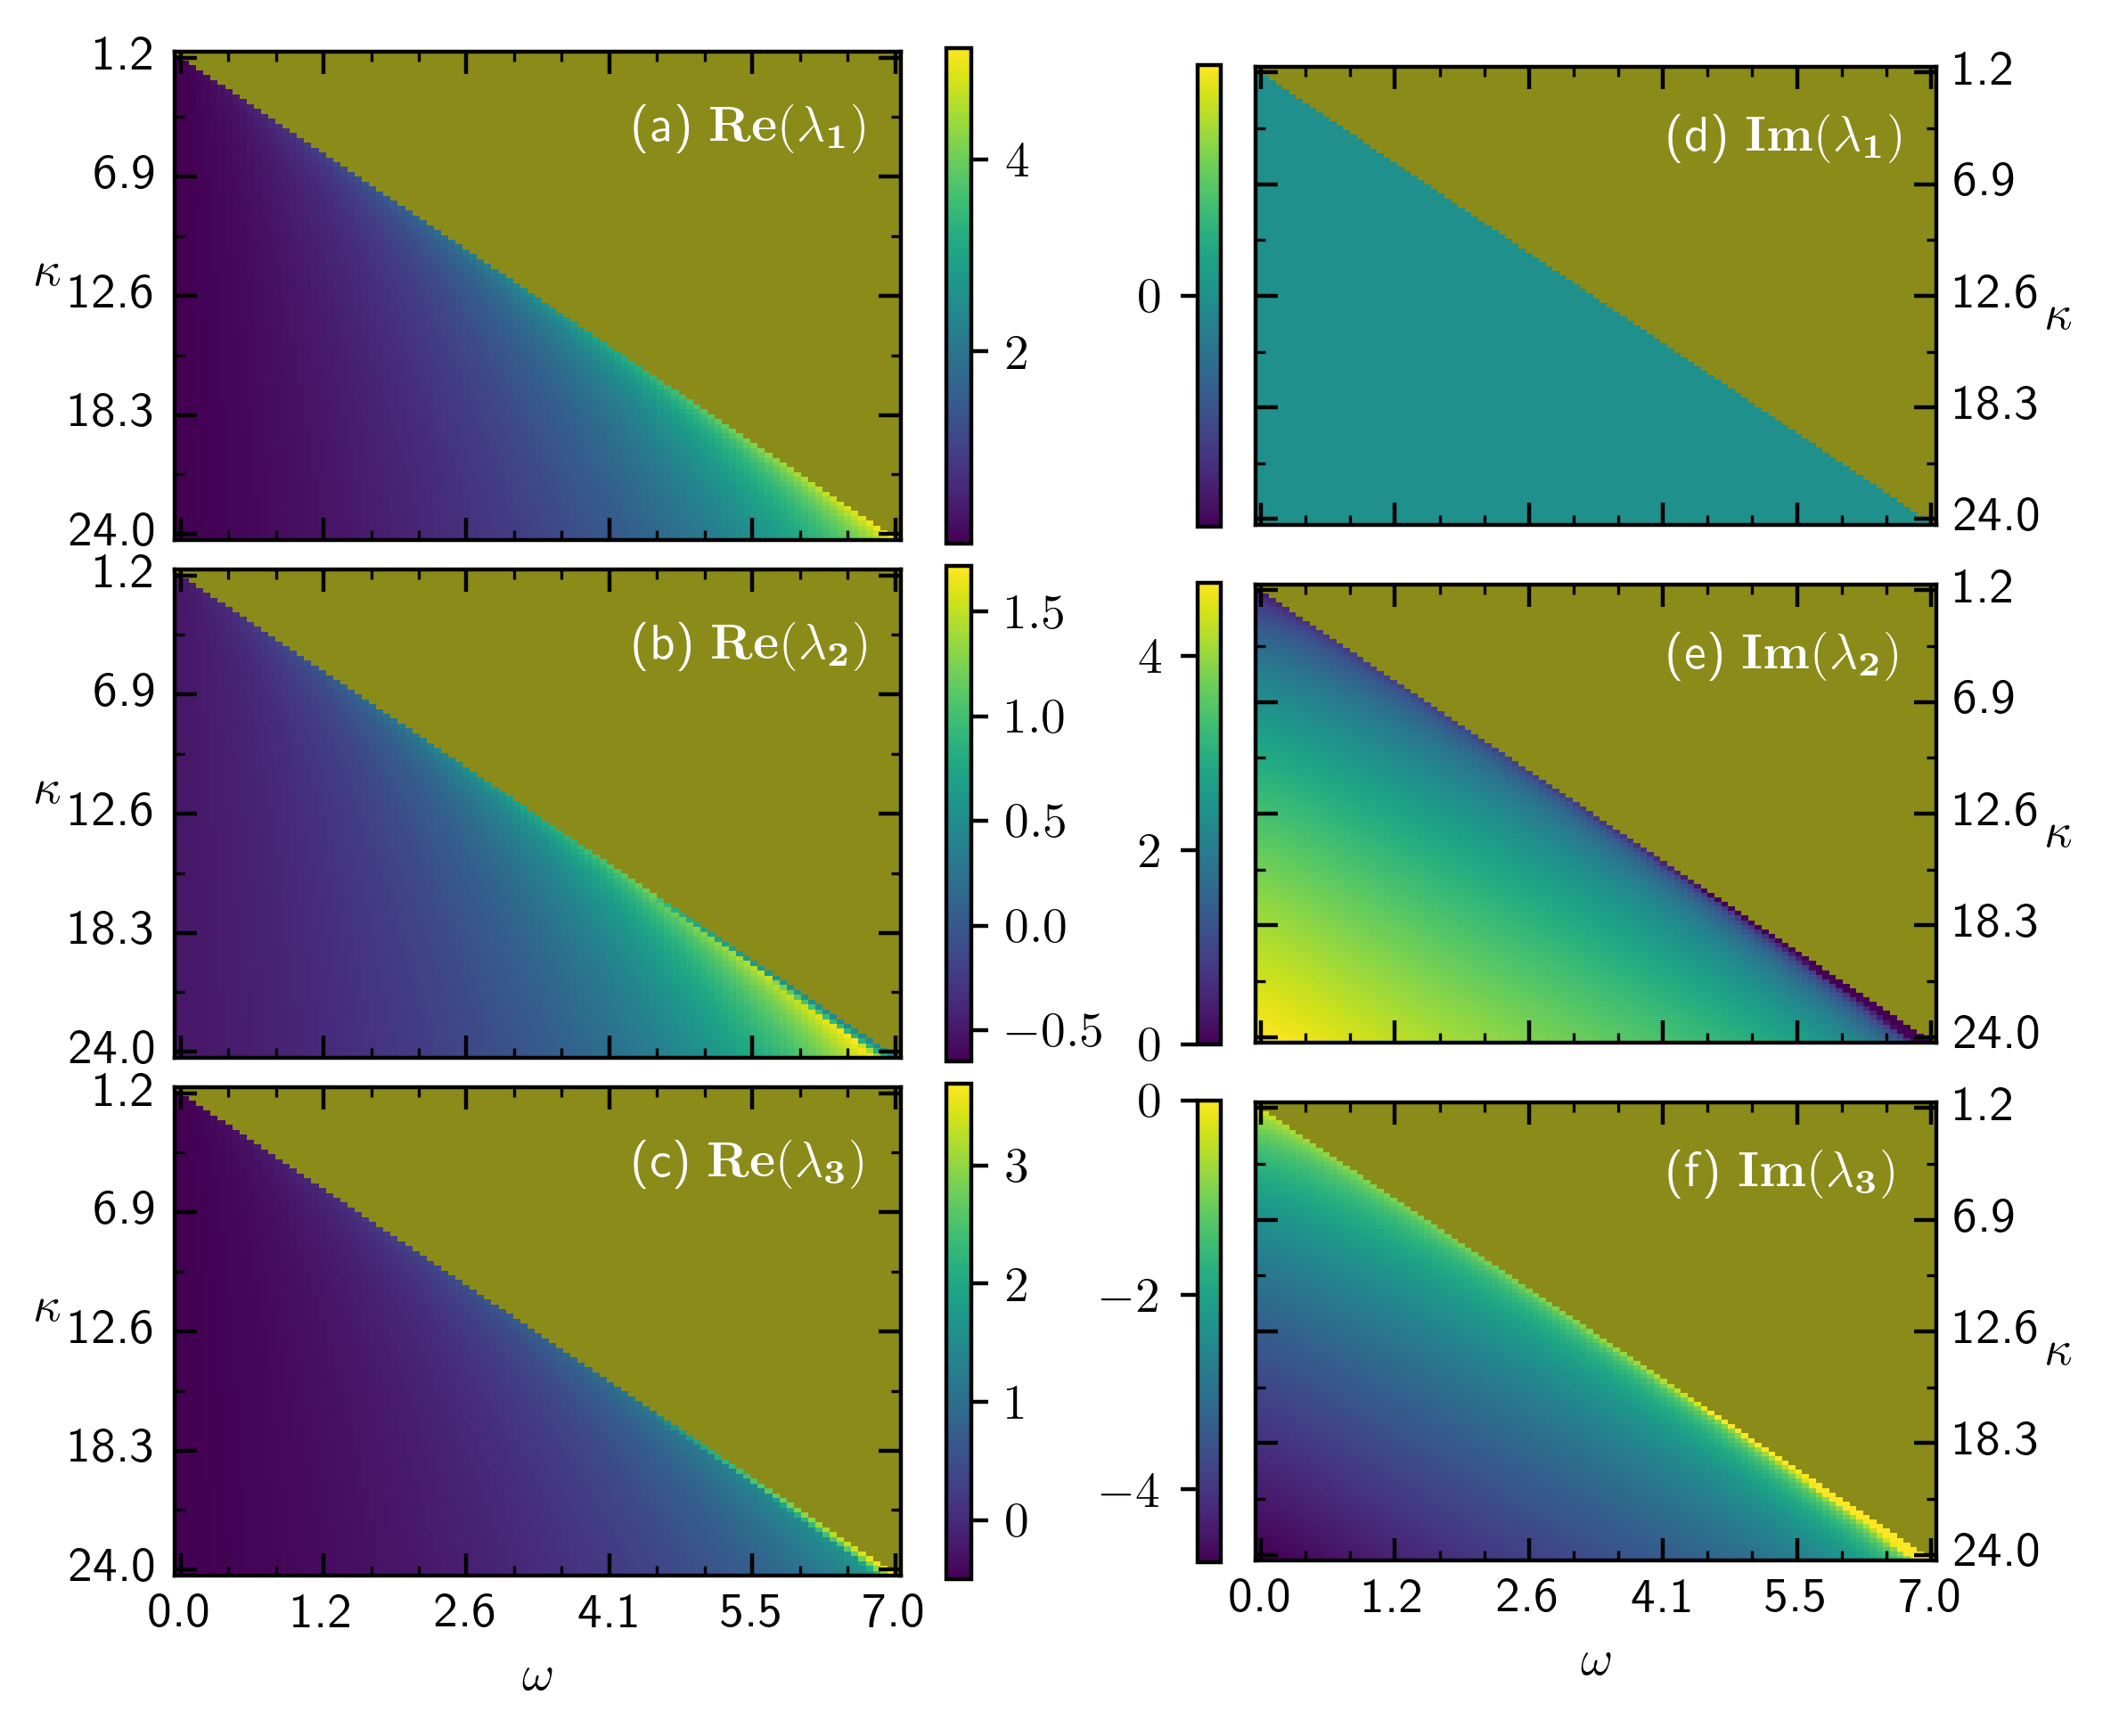
\includegraphics{pictures/lam_anal_l.png}
        \caption{Real and imaginary part of the eigenvalues from the linearization of the equations of motion are shown for the largest $y$-value fixed point.
        }
    \end{figure}
    
    \chapter{Appendix for the model with detuning}
    \section{Exemplary trajectories}
    \label{appendix:expl_traj}
    This paragraph shows a few exemplary long-time states of the system for the area where the transition of $m_x$-values is accompanied by multistability. Therefore I reconsider the outstanding regions in \figref{fig:fixedpoint_colormap} of \secref{sec:detuned_analysis}. I divide those regions into 9 parts and select randomly a parameter configuration out of those areas. For a few random initial conditions I depict the resulting long-time states.
    \begin{figure}[H]
        \centering
        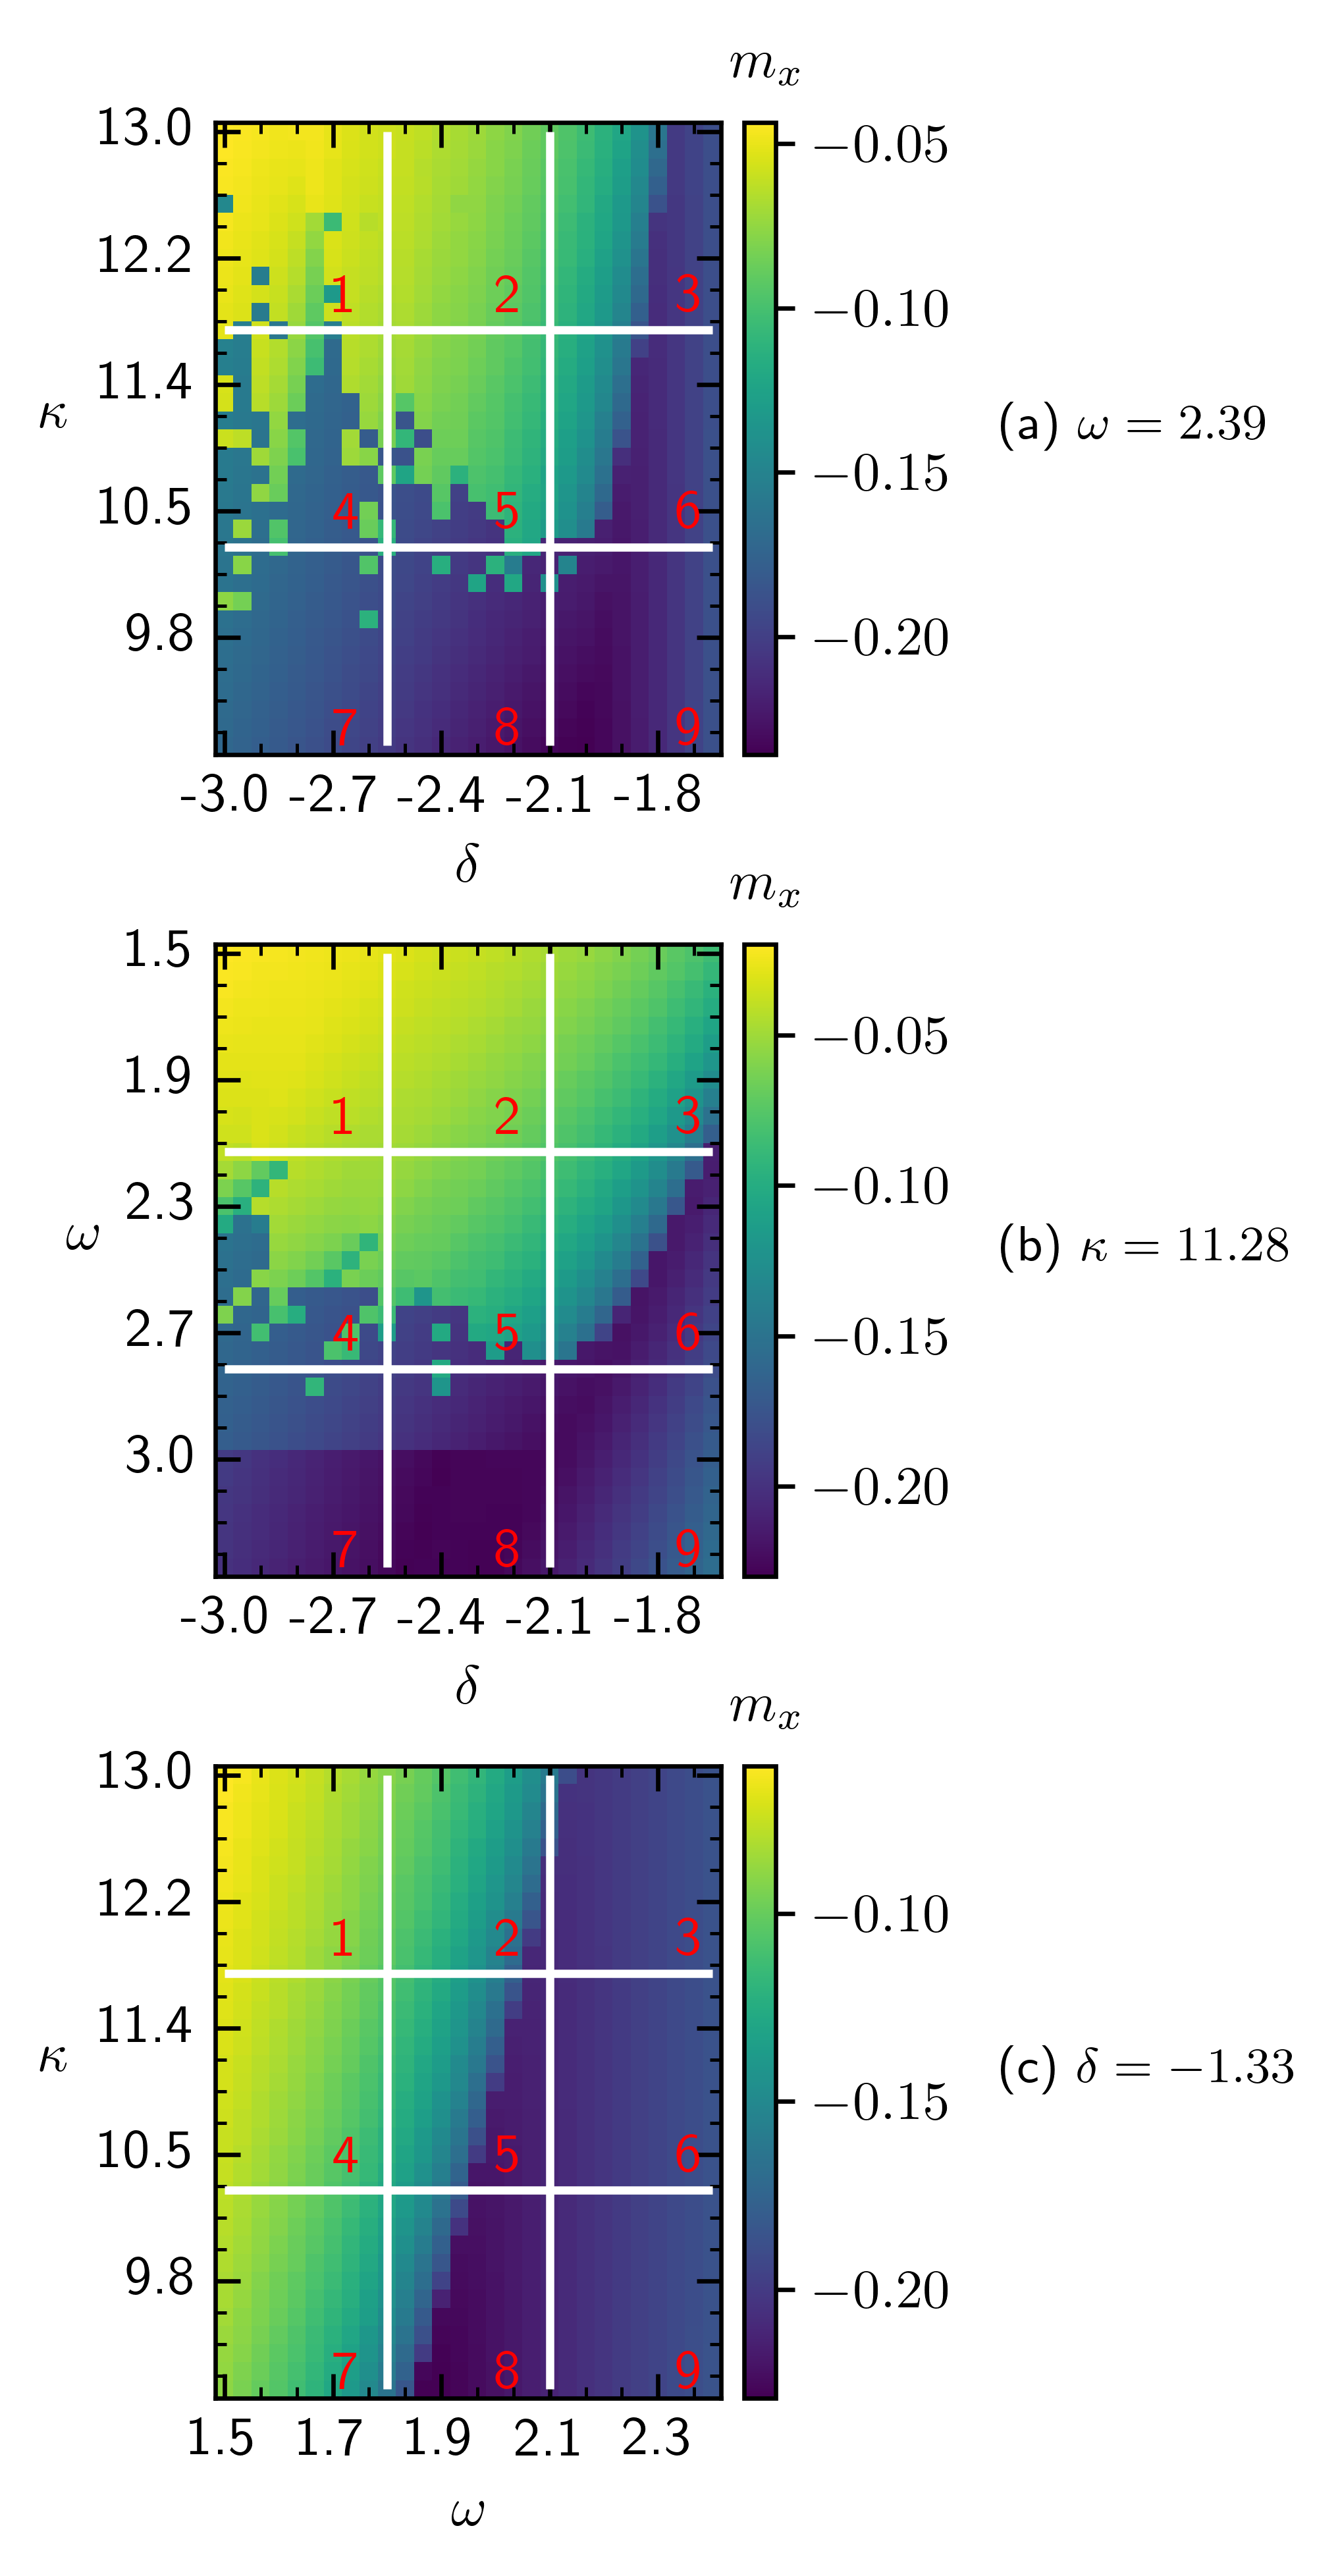
\includegraphics{pictures/combined_spec_sec.png}
        \caption{The division of the outstanding areas of \figref{fig:fixedpoint_colormap}.}
    \end{figure}
    
    \begin{figure}[H]
        \centering
        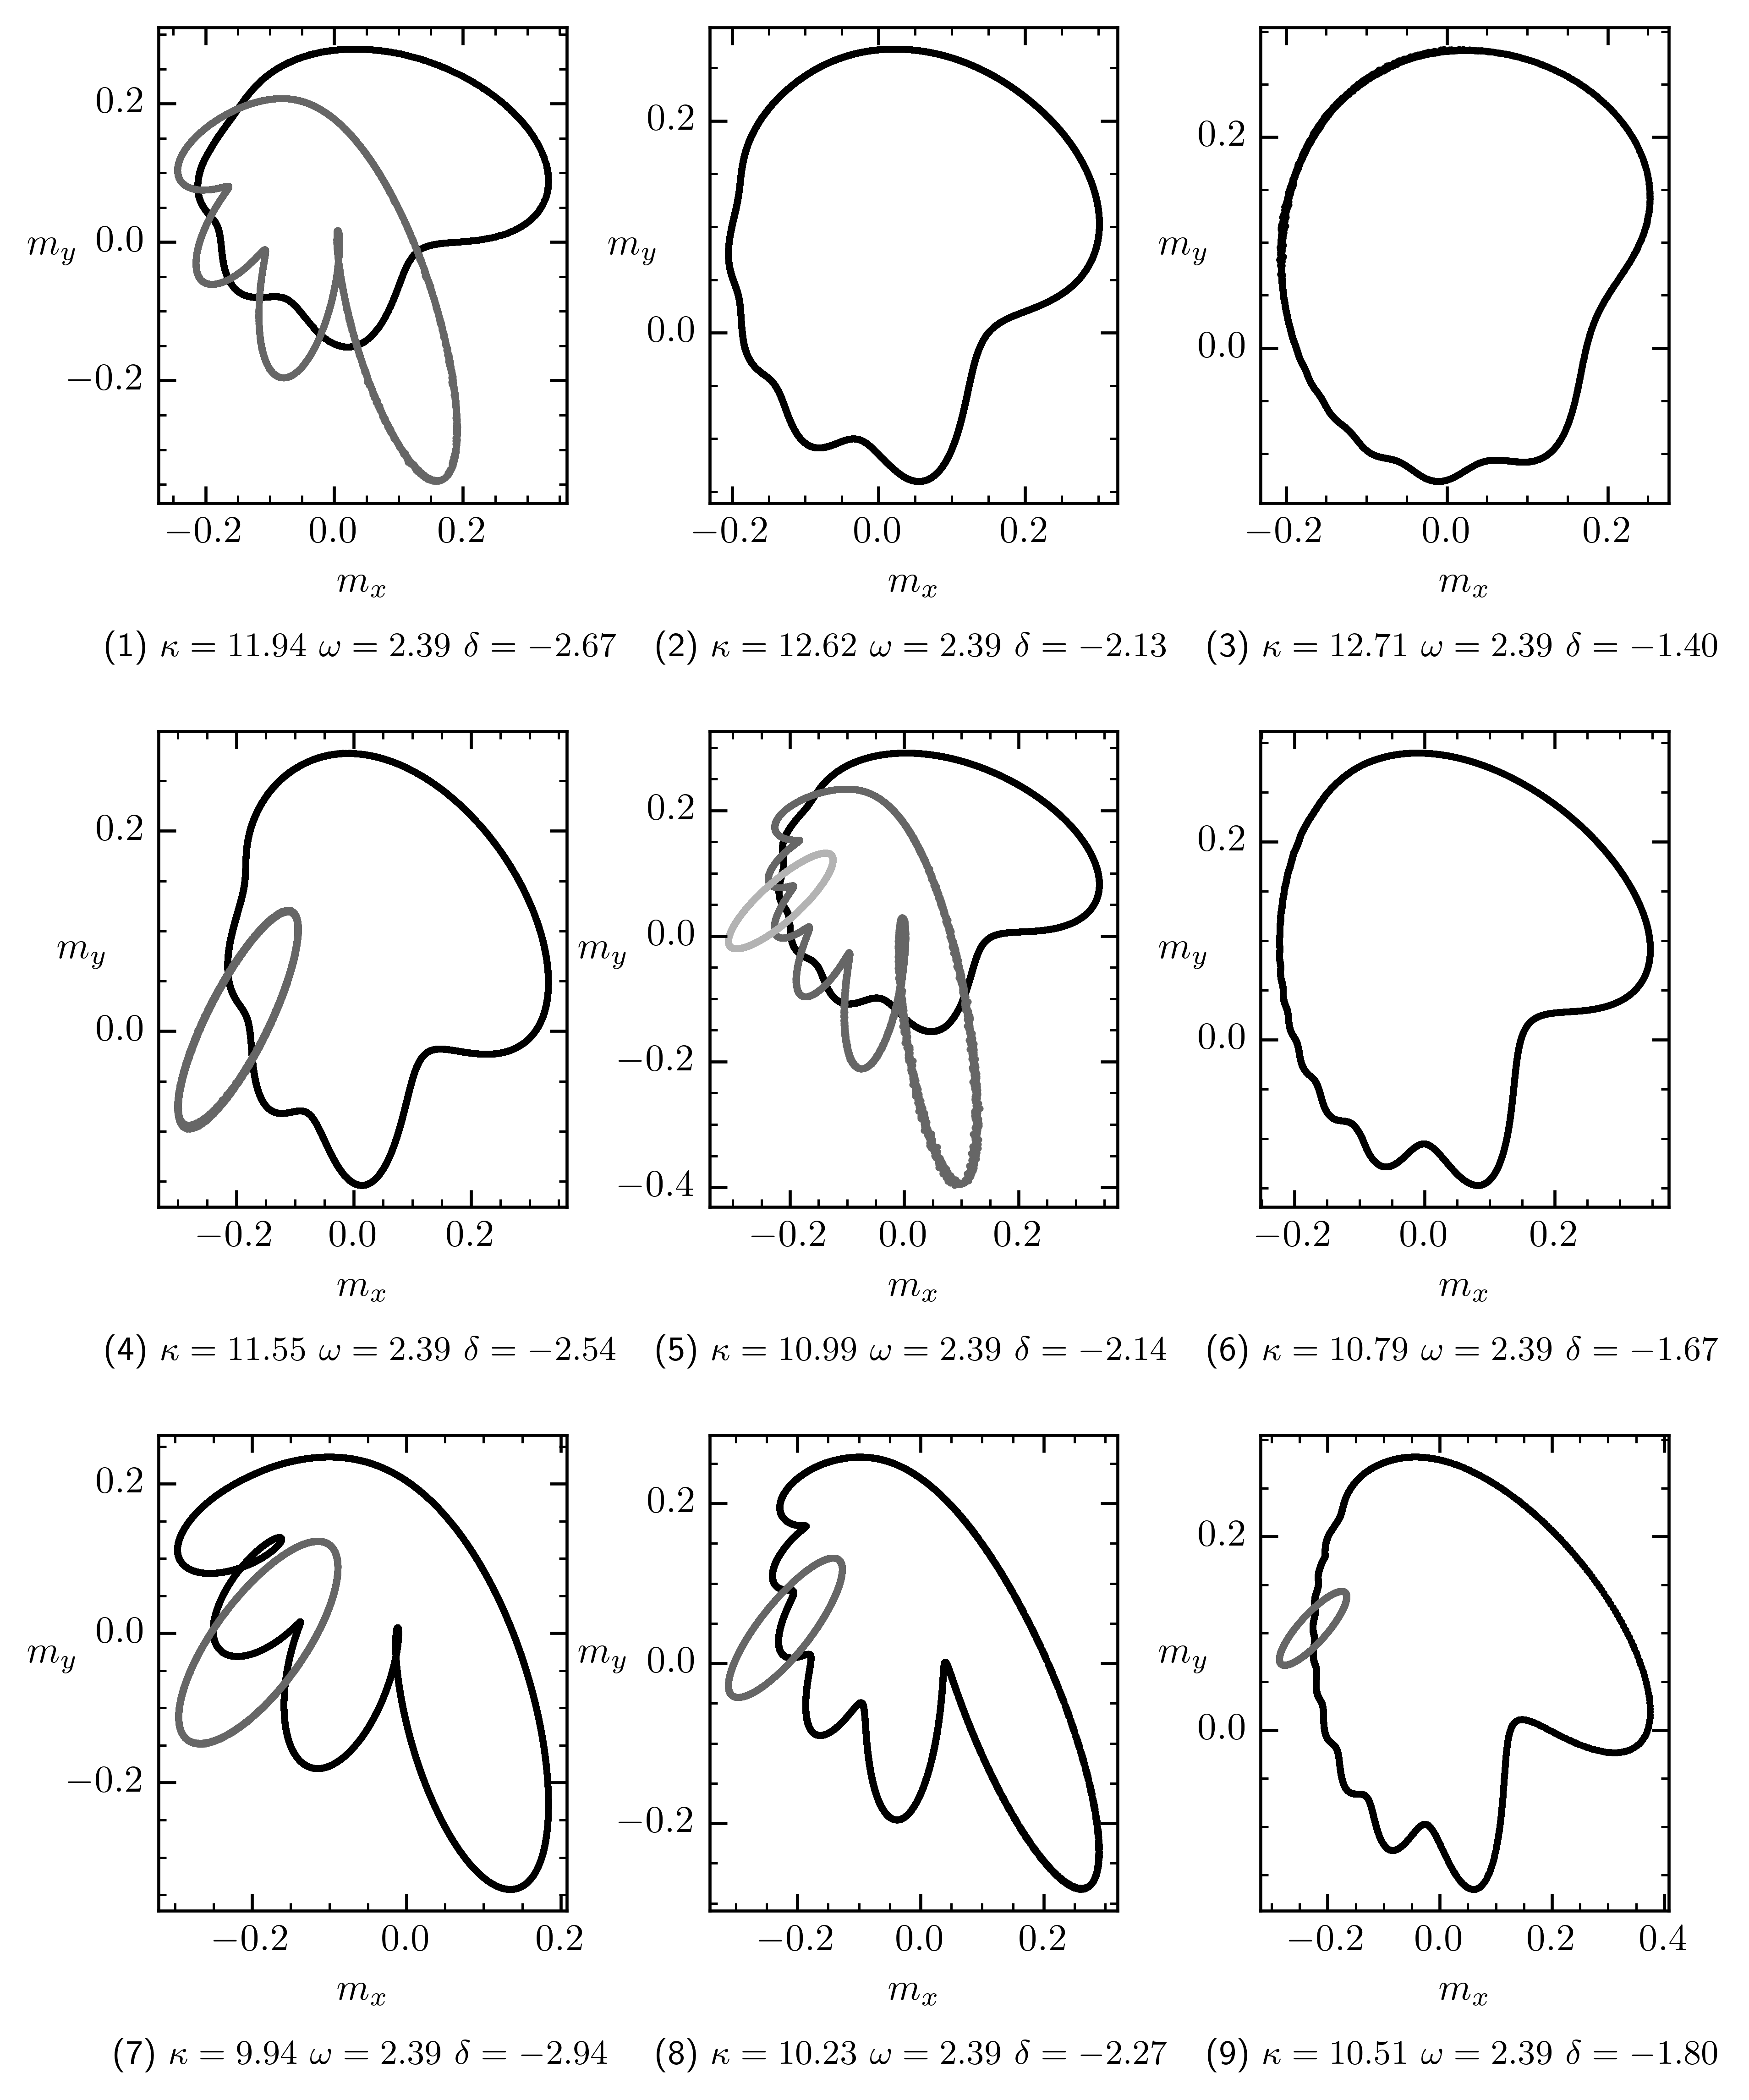
\includegraphics{pictures/lc_traj_wcut3.png}
        \caption{For $\omega=2.389$ possible long time states are shown for random values from the parameter grid. Where stationary points exist, I also drew the transition from the starting points to the stationary point.}
    \end{figure}
    
    \begin{figure}[H]
        \hspace*{-1cm}
        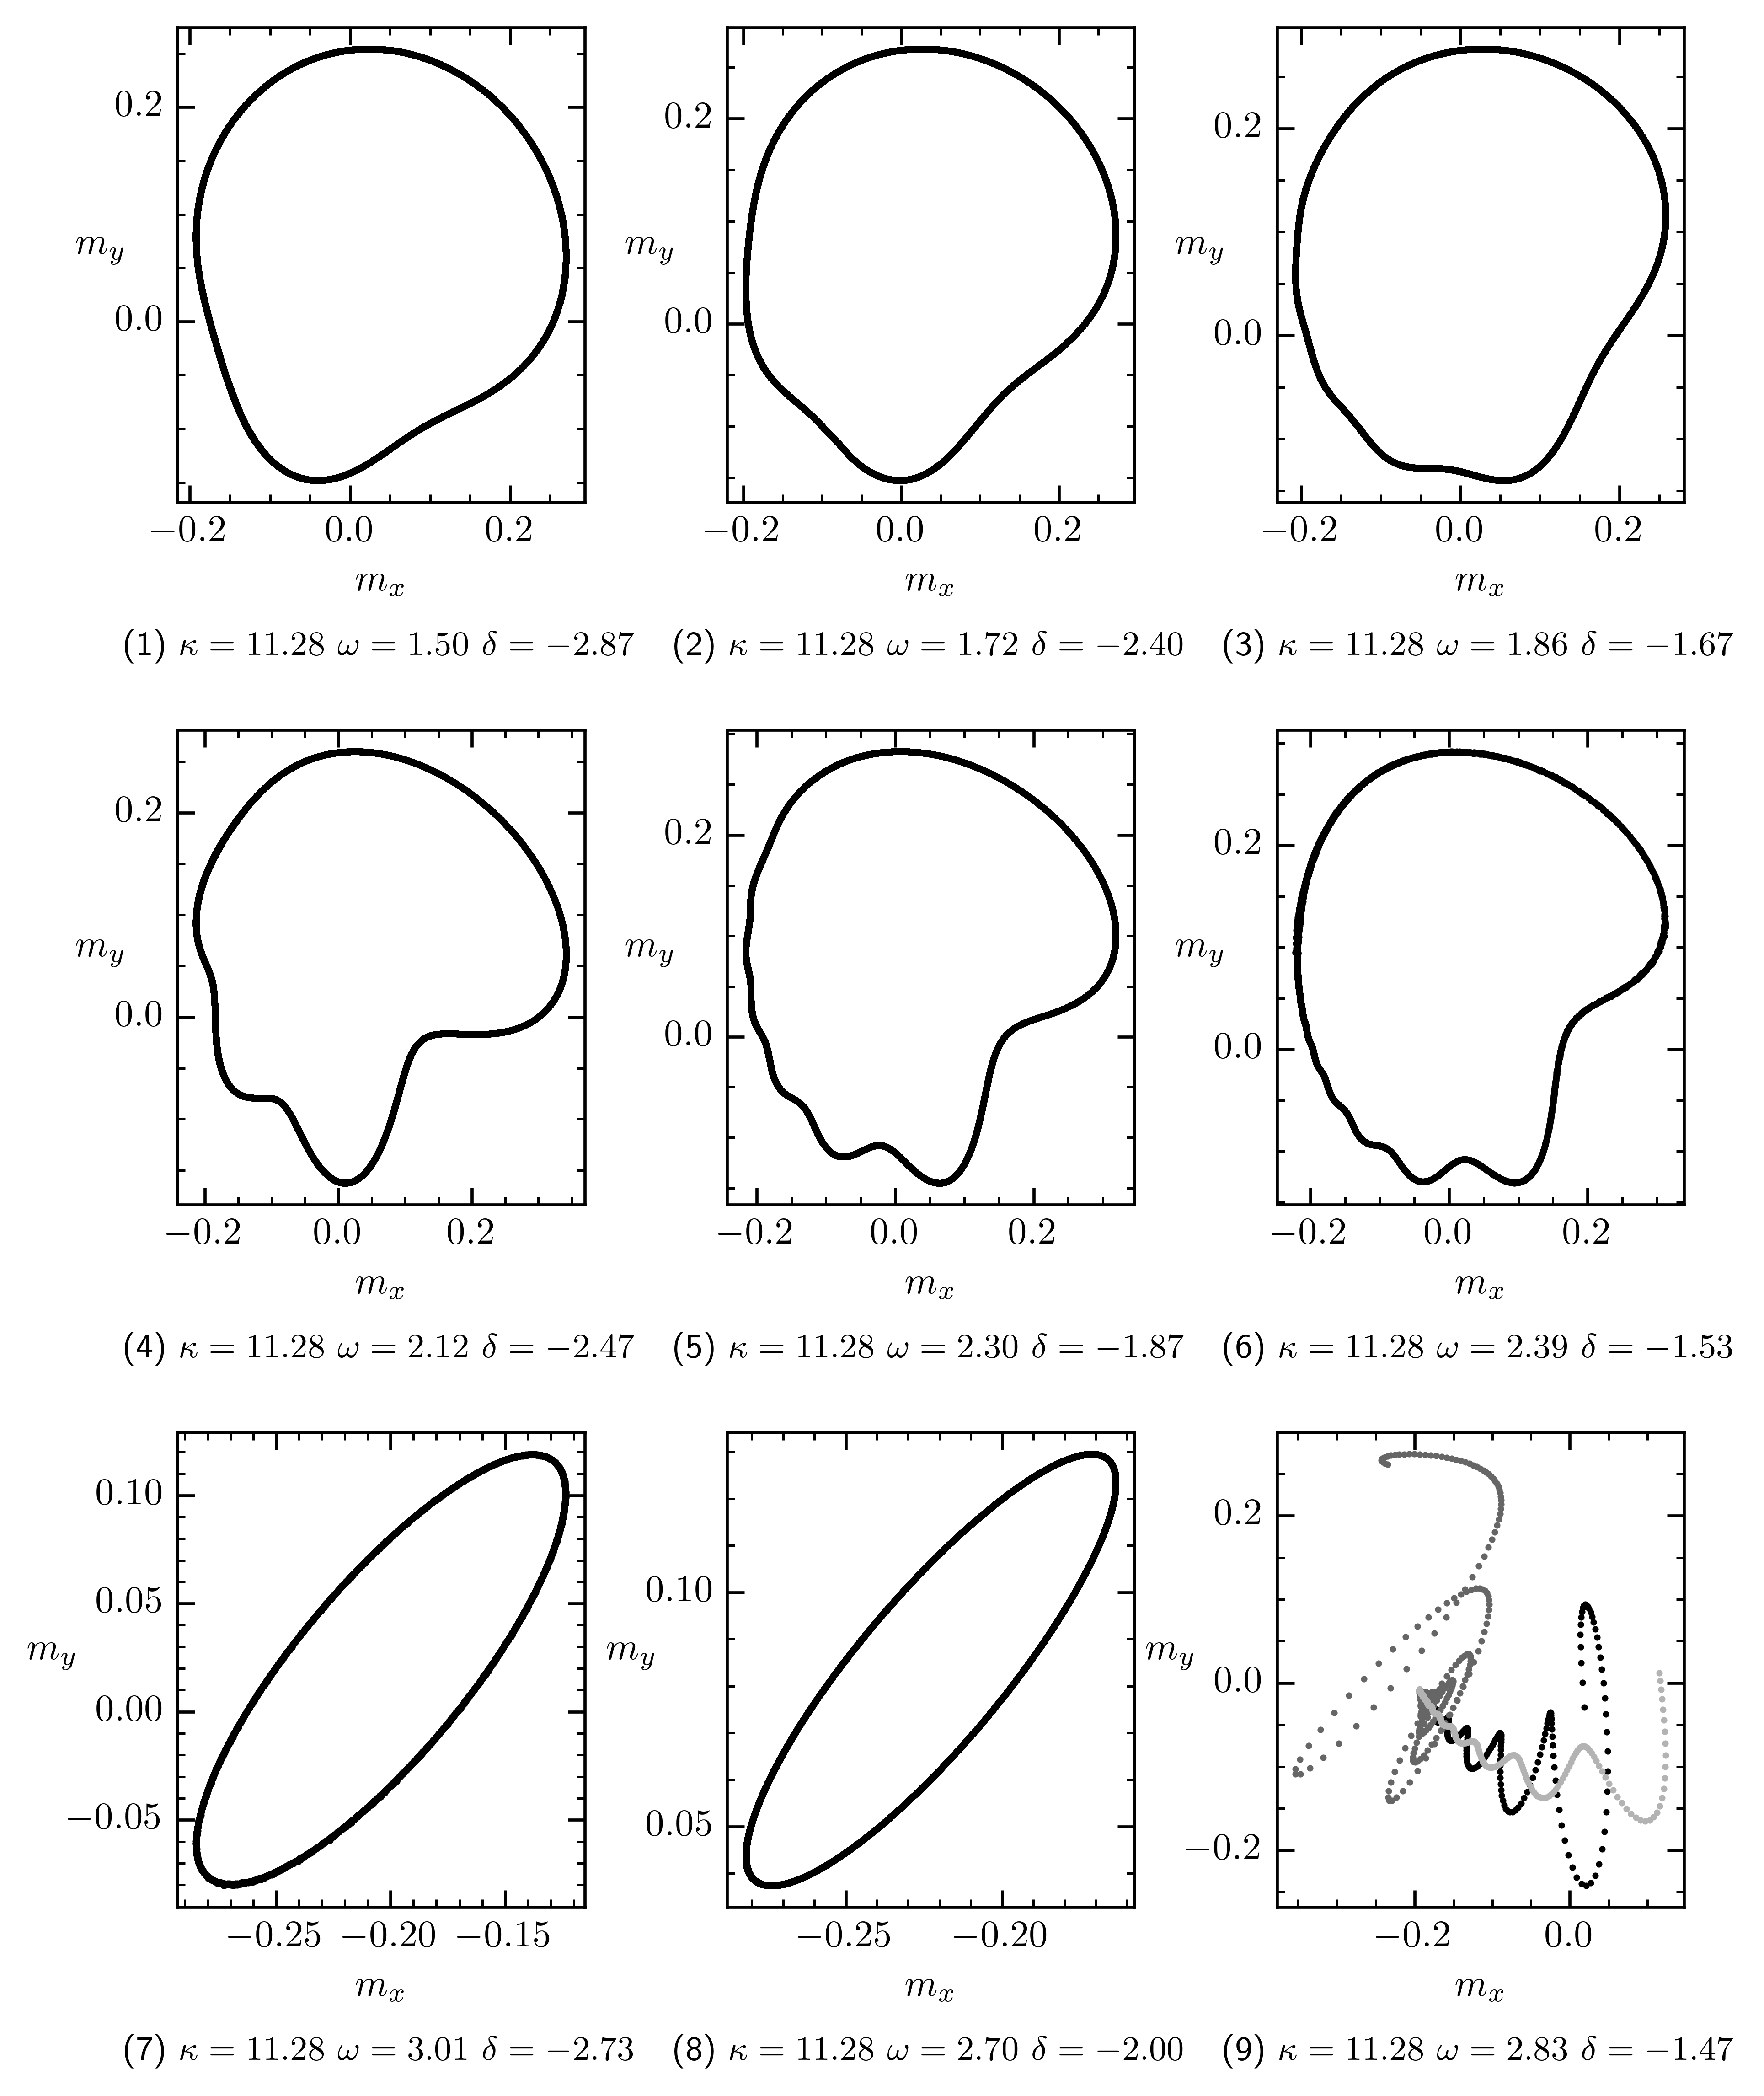
\includegraphics{pictures/lc_traj_kcut2.png}
        \caption{For $\kappa=11.28$ possible long time states are shown for random values from the parameter grid. Where stationary points exist, I also drew the transition from the starting points to the stationary point.}
    \end{figure}
    
    \begin{figure}[H]
        \centering
        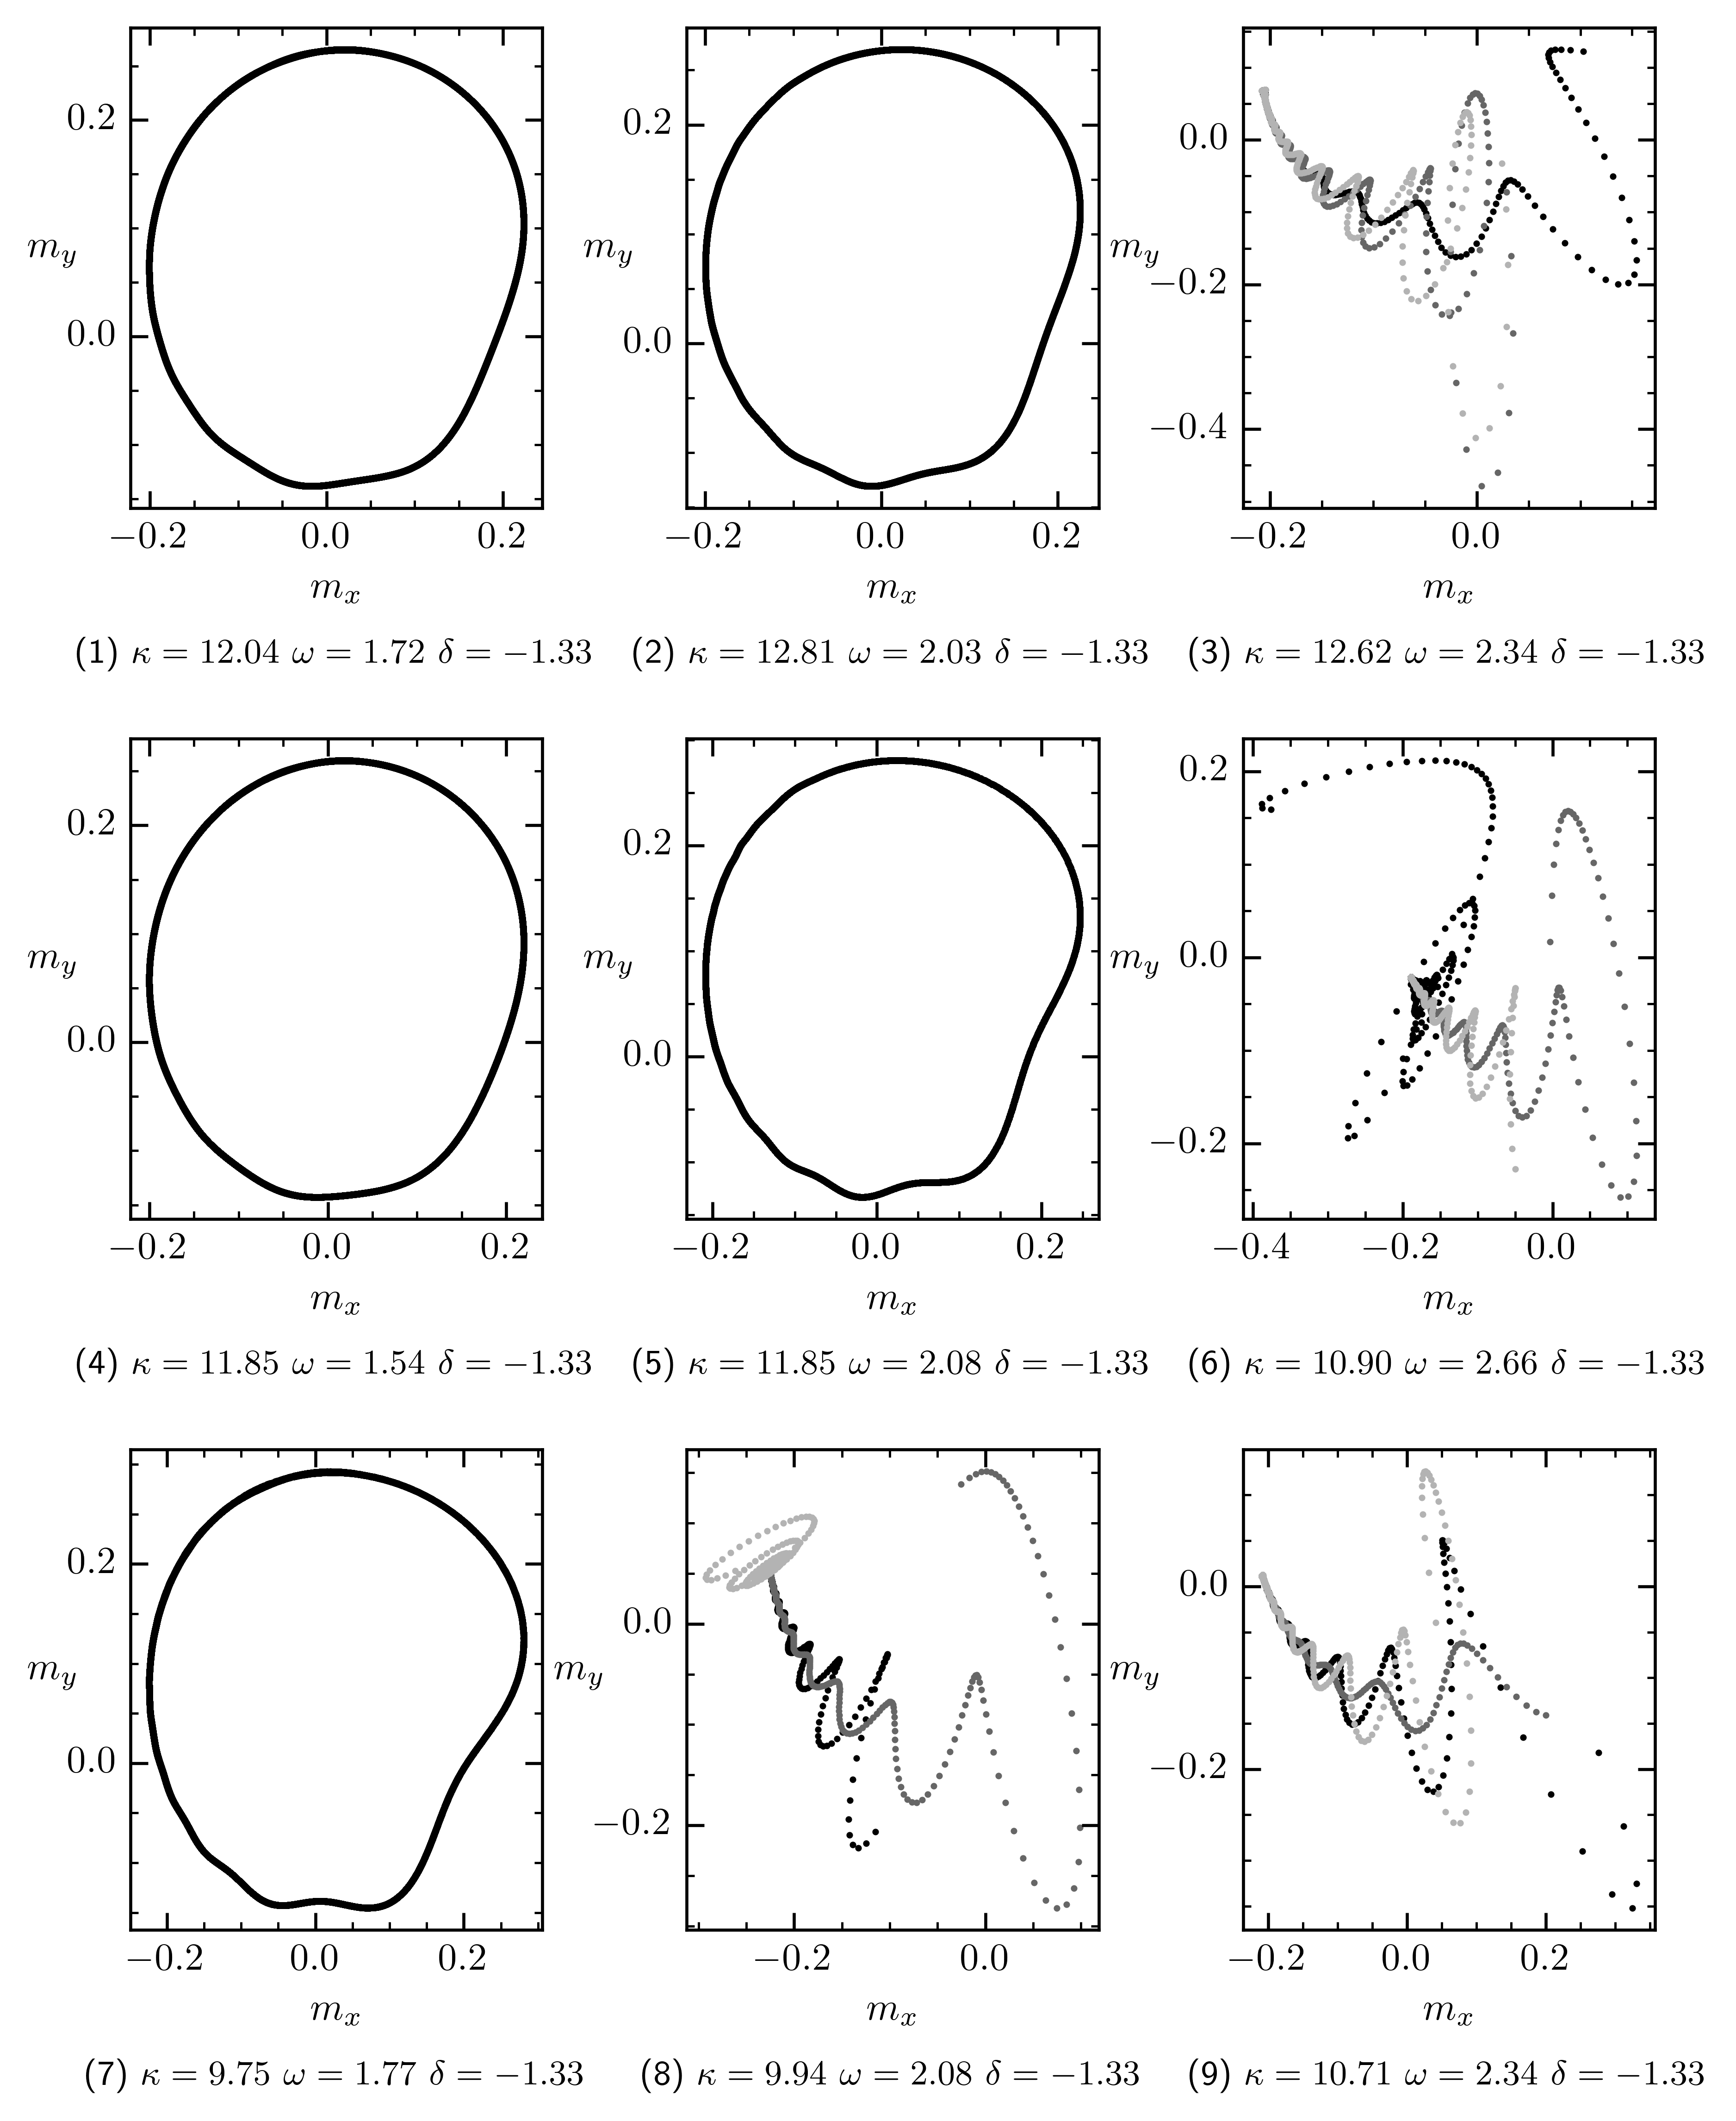
\includegraphics{pictures/lc_traj_dcut2.png}
        \caption{For $\delta=-1.33$ possible long time states are shown for random values from the parameter grid. Where stationary points exist, I also drew the transition from the starting points to the stationary point.}
    \end{figure}\newpage

    \section{Long-time states for varying dephasing strength}\label{app:gamma_analysis}
    An examination of the long-time states for different $\gamma$-values, which has been omitted in the main text, is briefly carried out at this point. For this purpose I again plot the stationary points as well as the average over a period of a limit cycle for different parameter values.
    \begin{figure}[H]
        \centering
        \caption{fixed points and averaged limit cycles over their period. In (a) $\gamma$ and $\delta$ are varied, while the other parameter a kept fixed. In (b) the cut with differing $\omega$ and $\delta$ is repeated for a different $\kappa$ and more importantly a different $\gamma$ value. $\Gamma=1$ as always. The white dashed line separates the region of limit cycles from that where stationary points exist. In both plots the area above the white line is the time crystal phase.}
        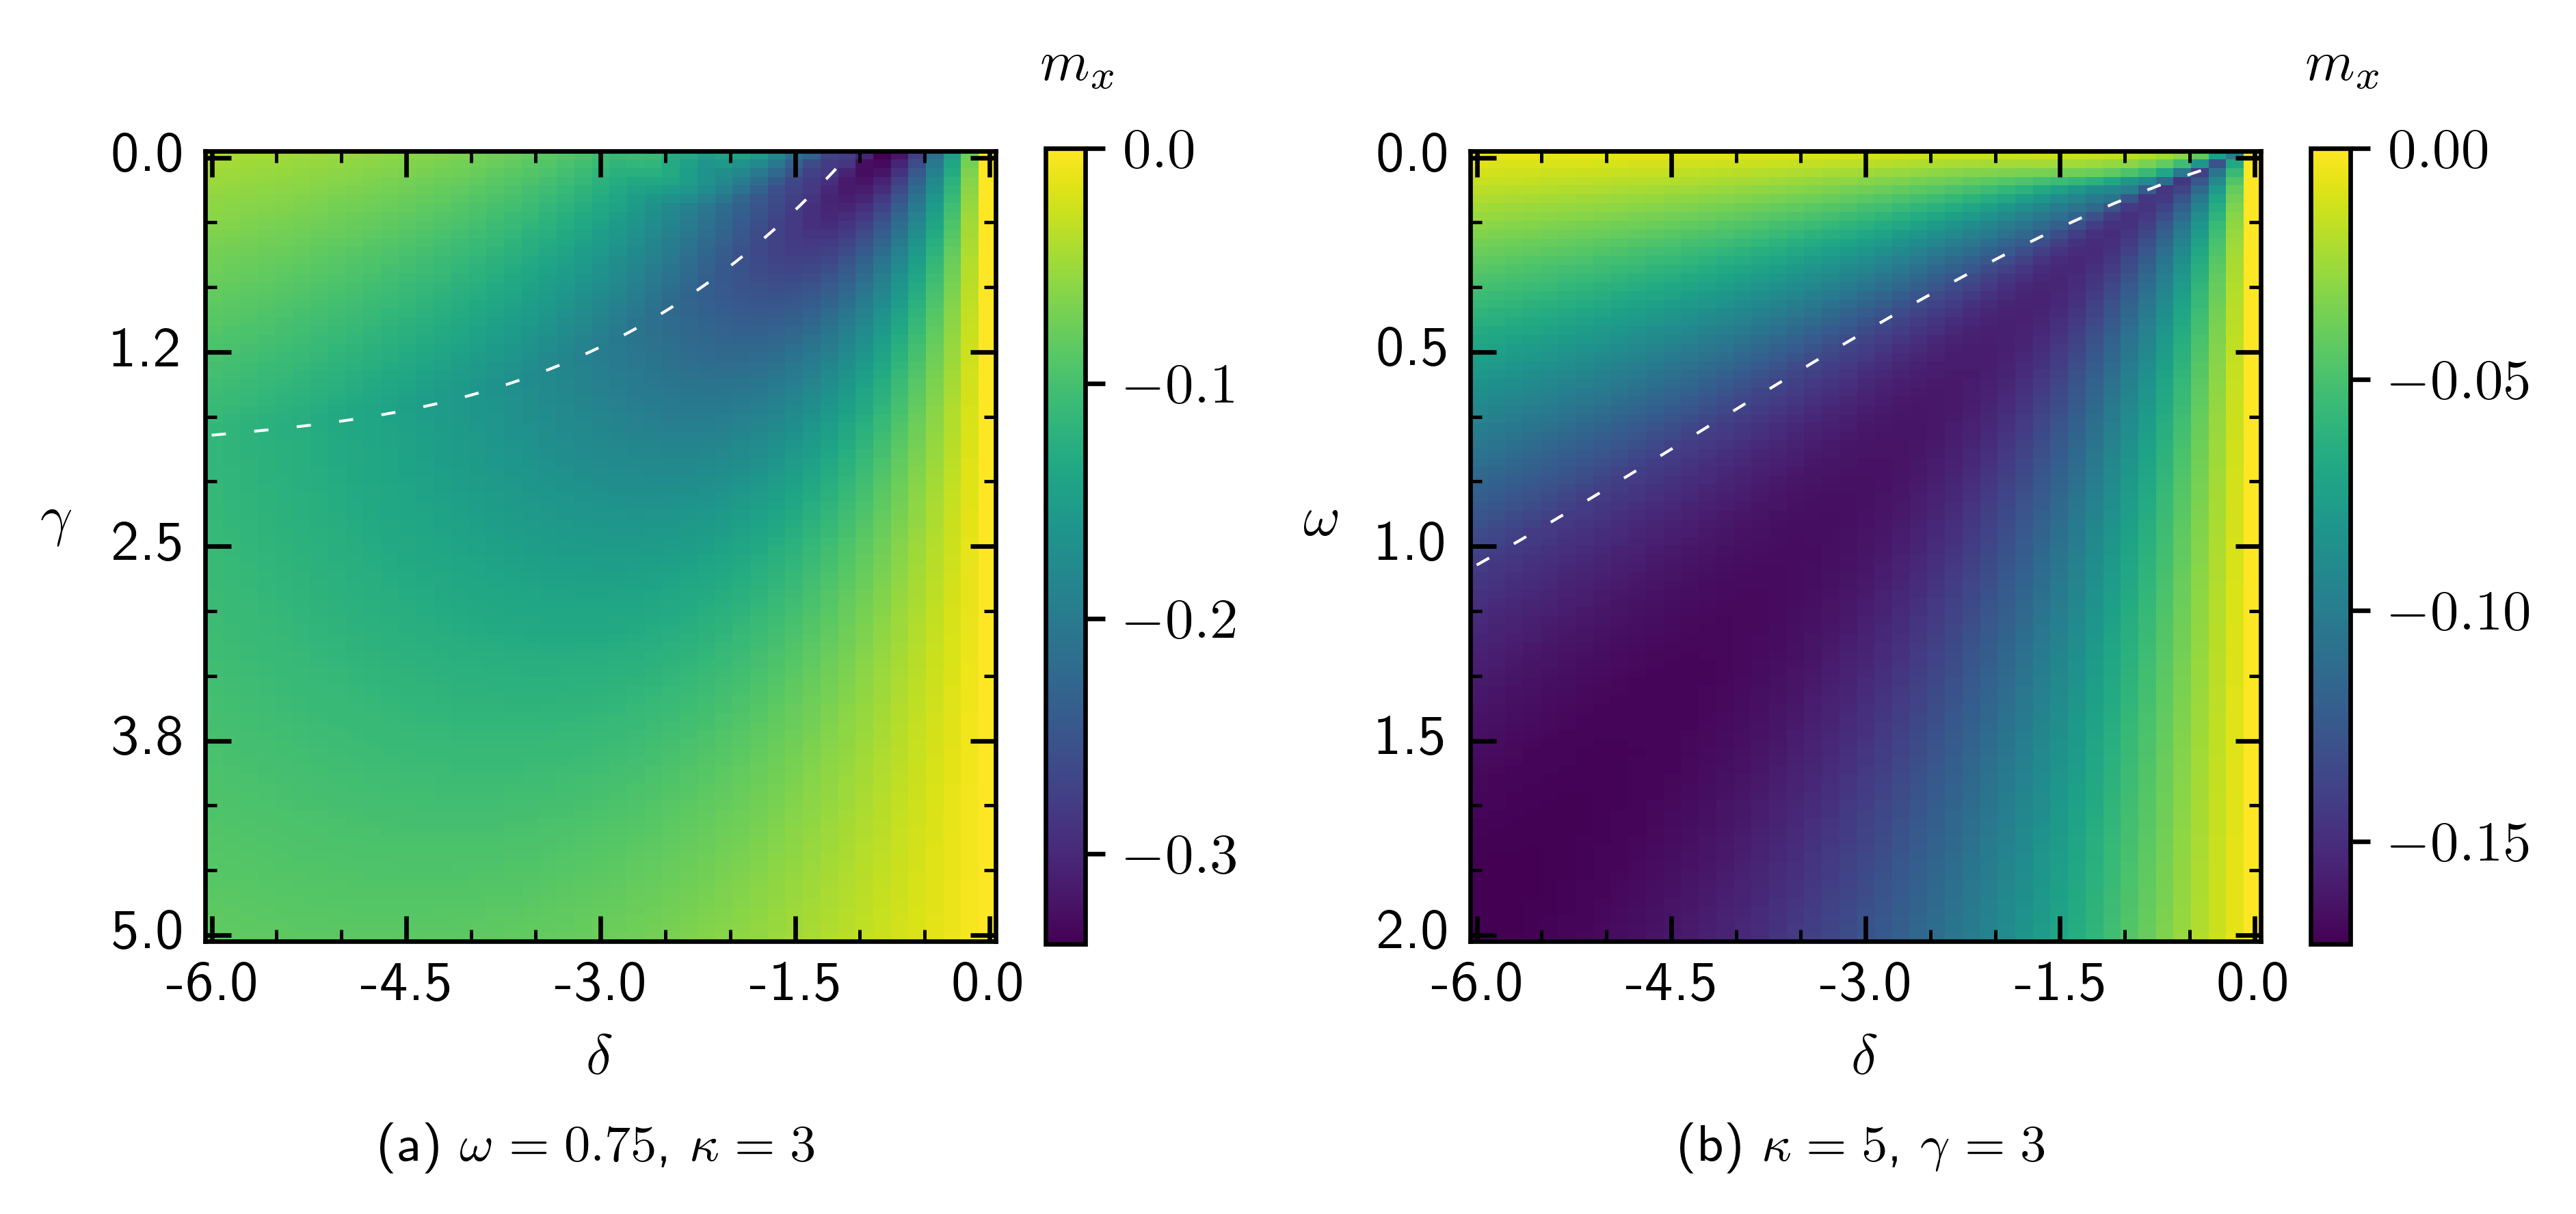
\includegraphics{pictures/limit_cycle_mean_gw.png}
        \label{fig:gamma_longtime}
    \end{figure}
    A several interesting observations can be made. Starting with \figref{fig:gamma_longtime}(b) one can see that the phase separation line has qualitatively the same shape as for $\gamma=0.2$. It again follows the property of synchronization effects that the larger the detuning between the considered systems is the larger the coupling between them has to be in order to see synchronization. I can also inform the reader that the parameter set that has been chosen in \figref{fig:gamma_longtime}  exhibits no multistability. For all configuration only one limit cycle or one stationary solution exists. \\
    What can be additionally observed is that the long-time states show a valley of small $m_x$ values, that lies near the phase separation line but does not coincide with it. \\\\
    Turning to \figref{fig:gamma_longtime}(a) one finds that the time crystal phase is stable for a wide range of dephasing strength for certain parameter constellations. What is also intriguing is that the higher $\gamma$ is the larger, in absolute value, the detuning has to be in order to observe a time crystal phase. The form of the phase separation line also suggests that there might be a maximal value of dephasing such that above that value no limit cycles can arise. But this definitively has to be yet verified, what could be an interesting subject of future analysis.




% \end{appendices}
\cleardoublepage

% additional material  
%%%%%%%%%%%%%%%%%%%%%%%%%%%%%%%%%%%%%%%%%%%%%%%%%%%%%%%%%%%%%%%%%%%%%%%%%%%%%%%%%%%%%%%%%%%%%%%%%

% {
% 	\thispagestyle{plain}
% 	\printbibliography
% 	\clearpage
% }

% % \begin{appendices}
\appendix
    \chapter{Appendix for the theoretical framework}
    \section{Derivation of the equations of motion}
    \label{appendix:eqm_derv}
    
    Starting from the Lindblad master equation I will derive the different interaction's contributions to the equations of motion for the components of the collective spin. For this purpose I
    revise a few of the properties of Pauli matrices.
    \begin{align*}
        [\sigma^\alpha,\sigma^\beta]&=2i\,\varepsilon_{\alpha\beta\lambda}\,\sigma^\lambda\\
        \Rightarrow\quad[J_\alpha,J_\beta]&=i\,\varepsilon_{\alpha\beta\lambda}\,J_\lambda\\
        [\sigma^z,\sigma^\pm]&=\pm2\,\sigma^\pm\\
        \Rightarrow\quad[J_z,J_\pm]&=\pm J_\pm\\
        \sigma^x\sigma^z&=\left( \begin{array}{cc}
             0 & -1  \\
             1& 0
        \end{array}\right)=-i\,\sigma^y\\
        \sigma^y\sigma^z&=\left( \begin{array}{cc}
             0 & i  \\
             i& 0
        \end{array}\right)=i\,\sigma_x\\
        \sigma^x\sigma^y&=\left( \begin{array}{cc}
             i & 0  \\
             0 & -i
        \end{array}\right)=i\,\sigma_z\\
        \sigma^\pm\sigma^z&=-i\,\sigma^y\pm i^2\,\sigma^x=\mp\sigma^\pm\\
        \sigma^-\sigma^+&=(\sigma^x)^2+(\sigma^y)^2+i\,\sigma^x\sigma^y-i\,\sigma^y\sigma^x\\
        &=2-2\,\sigma^z\\
        \sigma^+\sigma^-&=(\sigma^x)^2+(\sigma^y)^2-i\,\sigma^x\sigma^y+i\,\sigma^y\sigma^x\\
        &=2+2\,\sigma^z\\
        [\sigma^+,\sigma^-]_-&=4\,\sigma^z
    \end{align*}
    Applying these properties one can compute the part the driving is contributing to the equations of motion.
    \begin{align*}
        \mathcal{L}_\text{drive}(J_z)&=-i\,\omega\,\braket{[J_z,J_x]}\\
        &=\omega\,\braket{J_y}\\
        \mathcal{L}_\text{drive}(J_\pm)&=-i\,\frac{\delta}{2}\,\braket{[J_\pm,J_z]}-i\,\omega\,\braket{[J_\pm,J_x]}\\
        &=-i\,\left(\mp\frac{\delta}{2}\, \braket{J_\pm} \pm \omega\, \braket{J_z}\right)
    \end{align*}
    The contributions of the remaining interaction types can be also determined using the commutation relations.
    \begin{align*}
        \mathcal{L}_\text{SpE}(J_z)&=\frac{\kappa}{N}\,\Trs{\left(J_+ J_z J_- \rho-\half\,[J_z,J_+ J_-]_+\,\rho\right)}\\
        &=\frac{\kappa}{N}\,\Trs{\left(J_z J_+ J_- - J_+ J_- -\half\,(J_z J_+ J_- + J_+ J_z J_- + J_+ J_-)\right)\,\rho}\\
        &=\frac{\kappa}{N}\,\Trs{\left(J_z J_+ J_- - J_+ J_- -\half\,(2\,J_z J_+ J_- + J_+ J_- - J_+ J_-)\right)\,\rho}\\
        &=-\frac{\kappa}{N}\,\Trs{J_+ J_- \rho}
    \end{align*}

    \begin{align*}
        \mathcal{L}_\text{SpE}(J_+)&=\frac{\kappa}{N}\,\Trs{\left(J_+ J_+ J_- \rho-\half\,[J_+,J_+ J_-]_+\,\rho\right)}\\
        &=\frac{\kappa}{N}\,\Trs{\left(J_+ J_- J_+ + 2\,J_+ J_z -\half\,(J_+ J_- J_+ + J_+ J_+ J_-)\right)\,\rho}\\ &=\frac{\kappa}{N}\,\Trs{\left(J_+ J_- J_+ + 2\,J_+ J_z -\half\,(2\,J_+ J_- J_+ + 2 J_+ J_z)\right)\,\rho}\\\\
        &=\frac{\kappa}{N}\,\Trs{J_+ J_z \rho}\\\\
        \mathcal{L}_\text{SpE}(J_-)&=\frac{\kappa}{N}\,\Trs{\left(J_+ J_- J_- \rho-\half\,[J_-,J_+ J_-]_+\,\rho\right)}\\
        &=\frac{\kappa}{N}\,\Trs{\left(J_- J_+ J_- + 2\,J_z J_- -\half\,(J_- J_+ J_- + J_+ J_- J_-)\right)\,\rho}\\ 
        &=\frac{\kappa}{N}\,\Trs{J_z J_- \rho}
    \end{align*}
    \begin{align*}
        \mathcal{L}_\text{Dp}(J_z)&=0\\
        \mathcal{L}_\text{Dp}(J_\pm)&=\gamma\,\Trs{\left(J_z J_\pm J_z \rho-\half\,[J_\pm,J_z^2]_+\,\rho\right)}\\
        &=\gamma\,\Trs{\left(J_\pm J_z^2\rho \pm J_\pm J_z \rho-\half\,(J_\pm J_z^2 + J_z J_\pm J_z \pm J_z J_\pm)\,\rho\right)}\\
        &=\gamma\,\Trs{\left(J_\pm J_z^2\rho \pm J_\pm J_z \rho-\half\,(2\,J_\pm J_z^2  \pm J_z J_\pm \pm J_\pm J_z)\,\rho\right)}\\
        &=\pm\half\, \gamma\,\Trs{[J_\pm,J_z]\,\rho}\\
        &=-\half\,\gamma\,\Trs{J_\pm\rho}
    \end{align*}
    \begin{align*}
        \mathcal{L}_\text{pump}(J_z)&=\frac{\Gamma}{8}\,\sum_{j,k=1}^N \Trs{\left( \sigma_j^- \sigma_k^z \sigma_j^+ -\half\,[\sigma_k^z,\sigma_j^-\sigma_j^+]_+   \right)\,\rho}\\
        &=\frac{\Gamma}{8}\,\sum_{j,k=1}^N \Trs{\left( \sigma_j^- \sigma_k^z \sigma_j^+ -\half\,[\sigma_k^z\sigma_j^-\sigma_j^++\sigma_j^-\sigma_j^+\sigma_k^z]   \right)\,\rho}\\
        &=\frac{\Gamma}{8}\,\sum_{j,k=1}^N \Trs{\left( \sigma_j^- \sigma_k^z \sigma_j^+ -\half\,[2\,\sigma_j^-\sigma_k^z\sigma_j^+  -2\, \sigma_j^-\sigma_j^+\delta_{jk}-2\, \sigma_j^-\sigma_j^+\delta_{jk}]   \right)\,\rho}\\
        &=\frac{\Gamma}{8}\,\sum_{k=1}^N \Trs{2\, \sigma_k^-\sigma_k^+  \,\rho}\\
        &=\frac{\Gamma}{4}\,\sum_{k=1}^N \Trs{ (2-2\,\sigma_k^z)  \,\rho}\\
        &=\half\,N\,\Gamma-\Gamma\,\braket{J_z}
    \end{align*}
    \begin{align*}
        \mathcal{L}_\text{pump}(J_-)&=\frac{\Gamma}{4}\,\sum_{j,k=1}^N \Trs{\left( \sigma_j^- \sigma_k^- \sigma_j^+ -\half\,[\sigma_k^-,\sigma_j^-\sigma_j^+]_+   \right)\,\rho}\\
        &=\frac{\Gamma}{4}\,\sum_{k=1}^N \Trs{\left( \sigma_k^- \sigma_k^- \sigma_k^+ -\half\,[\sigma_k^-\sigma_k^-\sigma_k^++\sigma_k^-\sigma_k^+\sigma_k^-]   \right)\,\rho}\\
        &=-\frac{\Gamma}{2}\,\sum_{k=1}^N\Trs{\sigma_k^-\sigma_k^z\rho}\\
        &=-\frac{\Gamma}{2}\,\sum_{k=1}^N\Trs{\sigma_k^-\rho}\\\\
        \mathcal{L}_\text{pump}(J_+)&=\frac{\Gamma}{4}\,\sum_{j,k=1}^N \Trs{\left( \sigma_j^- \sigma_k^+ \sigma_j^+ -\half\,[\sigma_k^+,\sigma_j^-\sigma_j^+]_+   \right)\,\rho}\\
        &=-\frac{\Gamma}{2}\,\sum_{k=1}^N\Trs{\sigma_k^z\sigma_k^+\rho}\\
        &=-\frac{\Gamma}{2}\,\sum_{k=1}^N\Trs{\sigma_k^+\rho}
    \end{align*}
    
    \chapter{Appendix for zero detuning}
    \section{Decay without pumping}
    \label{appendix:msq_calc}
    In this paragraph I want to discuss, why in the absence of pumping the system always decays to fully mixed state. But first I want to derive a statement, which can be applied to certain driven-dissipative models, as they often encounter a similar form of the derivative  for the squared of the total spin. For this purpose assume that the coupled set of $N$ ordinary differential equations has the solution $\vec{F}:\,\mathbb{R}\rightarrow\mathbb{R}^N$. Define from that the function squared $F^2:\,\mathbb{R}\rightarrow\mathbb{R}:\,t\mapsto\sum_{i=1}^NF_i^2(t)$. The statement is now, that if one is able to write the derivative of the squared function in the following way
    \begin{align*}
        \half\,\dt F^2(t)&=\vec{F}^t(t)\,A\,\vec{F}(t)
    \end{align*}
    with a Matrix $A$, which is positive ore negative definite, then the only stationary solution to the system of ODE is $\vec{F}\equiv\vec{0}$. Further limit cycles can not exist. \\
    \textit{Proof}: The function $\vec{F}$, can be mapped via N-dimensional spherical coordinates into a different set of functions $f(t)$, $\varphi_j(t)$ $j\in\{1,\dots,N-1\}$, with $f$ the modulus of $F$, and $\varphi_j$ the angles. This is true for all solutions $\vec{F}\neq\vec{0}$. In the following I neglect this special case, as this is in the most cases anyway a stationary point and I am not interest in this part of the spin space. With the notation.
    \begin{align*}
        \vec{F}(t)&=f(t)\,\hat{r}(t)
    \end{align*}
    One can rewrite the differential equation for the squared function to
    \begin{align*}
        \half\,\dt F^2(t)=\half\,\dt f^2(t)=f(t)\,\dt f(t)&=f^2(t)\,\hat{r}^t\,A\,\hat{r}\\
        \Rightarrow\quad\dt f(t) = f(t)\,\hat{r}^t\,A\,\hat{r}
    \end{align*}
    Assuming that A is positive or negative definite one can use the property that $|\hat{r}(t)|=1\,\forall t$, in order to follow, that there exists an $\varepsilon>0$ so that
    \begin{align*}
        \lambda(t)\vcentcolon=\left| \hat{r}^t(t)\,A\,\hat{r}(t) \right| > \varepsilon
    \end{align*}
    For all $t$ and all functions $\{\varphi_j(t)\}$. \textit{Proof}: if this does not hold, there will have to be a sequence $(t_n)$ with $\lambda(t_n)\rightarrow0$. As the surface of an N-dimensional sphere is a compact set, this sequence would have to converge on the survace of the sphere, which would infer $\exists \hat{r}\neq0$ with 
    \begin{align*}
        \hat{r}^t(t)\,A\,\hat{r}(t)=0
    \end{align*}
    in contradiction to the definiteness of $A$. So depending on, whether $A$ is positive or negative definite, one can write
    \begin{align*}
        \dt f(t) >& \varepsilon\,f(t)\\
        \Rightarrow\quad f(t) >& c\,e^{\varepsilon\,t}\\
        \text{or}\quad \dt f(t) <& -\varepsilon\,f(t)\\
        \Rightarrow\quad f(t) <& c\,e^{-\varepsilon\,t}\\
    \end{align*}
    for suitable choice of $c$ (can be shown with mean value theorem). This implies, that there can't be a stationary solution of the set of ODE. The last statement holds, because for $t\rightarrow\infty$ either $f$ goes to zero, which would imply that all $F_i$ go to zero or $f$ grows boundlessly, which implies that, independent of the starting conditions, there exists a $F_i$, that grows boundlessly, which forbids the properties of a stationary state including limit cycles.\\\\Now in the case of the equations of motion in this work, the matrix $A$ is negative semi-definite in the absence of pumping. Nevertheless one can infer from the form of $A$ and the equations of motion that limit cycles can not exist and the only stationary state is $\vec{m}=0$. This can be seen by the following consideration. First revise the equations of motion for $\Gamma=0$
    \begin{align*}
        \dt m_x &= -\frac{\delta}{2}\,m_y-\half\,\gamma\,m_x+\kappa\,m_x m_z\\
        \dt m_y &= \frac{\delta}{2}\,m_x-\omega\,m_z-\half\,\gamma\,m_y+\kappa\,m_y m_z\\
        \dt m_z &= \omega\,m_y - \kappa\,(m_x^2+m_y^2)
    \end{align*}
    Accordingly the modulus of the total spin obeys the dynamics
    \begin{align*}
        \half\dt |m|^2=&-\half\,\hat{m}^t\,\left( \begin{array}{ccc}
            \gamma & 0&0  \\
            0& \gamma & 0\\
            0&0&0
       \end{array}\right)\,\hat{m}
    \end{align*}
    where $\hat{m}=\vec{m}/|m|$. In order for a vector to be a stationary solution, the derivatives of all spin components as well as the derivative of the total spin have to vanish. The latter condition implies $m_x=m_y=0$ and the combination with $\text{d}m_y/\text{d}t=0$ also demands $m_z=0$. Hence the fully mixed state is the only possible stationary point. Limit cycles can not exist either. This is found true by first noticing, that, because of the negative semi-definiteness of $A$, the total spin cannot grow. Thus in order for the system to have stable oscillations the total spin has to be constant, which implies that again $m_x=m_y=0$ has to hold. But this results in $m_z$ being constant. Hence no stable oscillations can occur.
    \newpage




    \section{Modulus of the fixed points in the case $\delta=0$}
    \label{appendix:mod_of_fixp}
    Here it is shown that all stationary solutions of the equations of motion without detuning are in the physically allowed set of values, i.e. $|m|\leq1/2$.
    The idea of the following analysis is to show first that $|m|$ is monoton in the parameters and then look at the maximum values. I begin by getting an expression for the modulus of the total spin.
    
    \begin{align*}
        m_z&=\half-\frac{1}{\Gamma}\,\left( \kappa\,(m_x^2+m_y^2)-\omega m_y  \right)\\
        &=\half-\frac{\kappa}{\Gamma}\,\left( m_y^2-\frac{\omega}{\kappa}\, m_y  \right)\\
        \Rightarrow\quad |m|^2&=\left( \half-\frac{\kappa}{\Gamma}\,\left( m_y^2-\frac{\omega}{\kappa}\, m_y  \right) \right)^2+m_y^2\\
        &=\left( \half-\frac{\omega^2}{\Gamma\kappa}\,\left( {y}^2- {y} \right) \right)^2+\frac{\omega^2}{\kappa^2}\,{y}^2\\
        &=\left( \half-\frac{\Omega^2}{K}\,\left( {y}^2- {y} \right) \right)^2+\frac{\Gamma}{\Gamma+\gamma}\,\frac{\Omega^2}{K^2}\,{y}^2\\
        \leq&\left( \half-\frac{\Omega^2}{K}\,\left( {y}^2- {y} \right) \right)^2+\frac{\Omega^2}{K^2}\,{y}^2\\
        &=\vcentcolon m^*
    \end{align*}
    The last definition allows to continue the analysis with only two parameters $K$, $\Omega$. The real magnetic modulus squared is always smaller than $m^*$. In order to take into account the interdependence of $y$ and the parameters through the determining equation for $y$, I have to express them through each other. 
    \begin{align*}
        0&=F(y)=-\frac{K}{2\Omega^2}-\left( \frac{1-K}{2\Omega^2} +1\right)\,{y}-{y}^3+2\,{y}^2\\
        \Rightarrow\quad \frac{K}{2\Omega^2}\,({y}-1)&=(1+\frac{1}{2\Omega^2})\,{y}+{y}^3-2\,{y}^2\\
        \frac{\Omega^2}{K}&=\frac{{y}-1}{2\,\left(  (1+\frac{1}{2\Omega^2})\,{y}+{y}^3-2\,{y}^2\right)}
    \end{align*}
    This equation looks at first strange, because $K/2\Omega^2$ could be negative for $0<{y}<1$. But as has been already seen in \figref{fig:sign_lam1}, this space is free of fixed points. For the computation of the derivative of $m^*$, the following is useful. 
    \begin{align*}
        \frac{\text{d}}{\text{d}{y}}\,\frac{\Omega^2}{K}&=\frac{1}{2\,\left(  (1+\frac{1}{2\Omega^2})\,{y}+{y}^3-2\,{y}^2\right)}-\frac{2\,({y}-1)\,(1+\frac{1}{2\Omega^2}+3\,{y}^2-4\,{y})}{4\,\left(  (1+\frac{1}{2\Omega^2})\,{y}+{y}^3-2\,{y}^2\right)^2}\\\\
        &=\frac{1+\frac{1}{2\Omega^2}-4\,{y}+5\,{y}^2-2\,{y}^3}{2\,\left(  (1+\frac{1}{2\Omega^2})\,{y}+{y}^3-2\,{y}^2\right)^2}
    \end{align*}
    The derivative of $m^*$ is calculated via
    \begin{align*}
        \frac{\partial m^*}{\partial{y}}&=-2\,\left(\frac{\Omega^2}{K}\,(2{y}-1)+\left(\frac{\text{d}}{\text{d}{y}}\,\frac{\Omega^2}{K}\right)\,({y}^2-{y})\right)\,\left( \half-\frac{\Omega^2}{K}\,\left( {y}^2- {y} \right) \right)+2\,\frac{\Omega^2}{K^2}\,{y}+2\,\left(\frac{\text{d}}{\text{d}{y}}\,\frac{\Omega^2}{K}\right)\,\frac{\Omega^2}{K}\,\frac{1}{\Omega^2}\,{y}^2\\\\
        &=4\,(\frac{\Omega^2}{K})^2\,{y}^3-\left(2\,(\frac{\Omega^2}{K})^2+4\,(\frac{\Omega^2}{K})^2\right)\,{y}^2+\left( 2\,(\frac{\Omega^2}{K})^2+2\,\frac{\Omega^2}{K^2}-2\,\frac{\Omega^2}{K} \right)\,{y}+\frac{\Omega^2}{K}\\\\
        &+2\,\dkw\,\kw\,{y}^4-4\,\dkw\,\kw\,{y}^3\\\\
        &-\left(\dkw-2\,\dkw\,\kw-2\,\dkw\,\kw\,\frac{1}{\Omega^2}\right)\,{y}^2+\dkw\,{y}\\\\
        &=\frac{\Omega^2}{K}\,\left[  4\,\frac{\Omega^2}{K}\,{y}^3-6\,\frac{\Omega^2}{K}\,{y}^2+\left( 2\,\frac{\Omega^2}{K}+2\,\frac{\Omega^2}{K}\,\frac{1}{\Omega^2}-2 \right)\,{y}+1 \right]\\\\
        &+\dkw\,\left[2\,\kw\,{y}^4-4\,\kw\,{y}^3-\left(1-2\,\kw-2\,\kw\,\frac{1}{\Omega^2}\right)\,{y}^2+{y}\right]\\\\
        &=\vcentcolon \frac{\partial \alpha}{\partial{y}}+\dkw\,\frac{\partial \beta}{\partial{y}}
    \end{align*}
    
    Plugging the former expression into the equation for the derivative of $m^*$ yields
    \begin{align*}
        \frac{2\,\left[(1+\frac{1}{2\Omega^2})\,{y}+{y}^3-2\,{y}^2\right]^2}{{y}-1}\,\frac{\partial \alpha}{\partial{y}}&=2\,({y}-1)\,{y}^3-3\,({y}-1)\,{y}^2\\
        &+\left( {y}-1+({y}-1)\,\frac{1}{\Omega^2}-2\,\left((1+\frac{1}{2\Omega^2})\,{y}+{y}^3-2\,{y}^2\right) \right)\,{y}\\
        &+(1+\frac{1}{2\Omega^2})\,{y}+{y}^3-2\,{y}^2 \\\\
        &=3\,{y}^2+\left( -(1+\frac{1}{\Omega^2})-{y}\right)\,{y}+(1+\frac{1}{2\Omega^2})\,{y}-2\,{y}^2\\
        &=-\frac{1}{2\Omega^2}\,{y}\\\\
        \Rightarrow\quad\frac{\partial \alpha}{\partial{y}}&=-\frac{{y}-1}{2\,\left[(1+\frac{1}{2\Omega^2})\,{y}+{y}^3-2\,{y}^2\right]^2}\,\frac{1}{2\Omega^2}\,{y}
    \end{align*}
    Doing the same for the $\beta$-expression, one finds
    \begin{align*}
        \left[(1+\frac{1}{2\Omega^2})\,{y}+{y}^3-2\,{y}^2\right]\,\frac{\partial \beta}{\partial{y}}&=({y}-1)\,{y}^4-2\,({y}-1)\,{y}^3-\left( (1+\frac{1}{2\Omega^2})\,{y}+{y}^3-2\,{y}^2-{y}+1-({y}-1)\,\frac{1}{\Omega^2} \right)\,{y}^2\\
        &+((1+\frac{1}{2\Omega^2})\,{y}+{y}^3-2\,{y}^2)\,{y}\\
        &=-\left( 1+\frac{1}{\Omega^2}-\frac{1}{2\Omega^2}\,{y}  \right)\,{y}^2+(1+\frac{1}{2\Omega^2})\,{y}^2\\
        &=\frac{1}{2\Omega^2}\,({y}^3-{y}^2)=\frac{1}{2\Omega^2}\,{y}^2\,({y}-1)
    \end{align*}
    After joining all terms, one finds
    \begin{align*}
        \frac{\partial \alpha}{\partial{y}}+\dkw\,\frac{\partial \beta}{\partial{y}}&=-\frac{\frac{1}{2\Omega^2}\,({y}-1)}{2\,\left[(1+\frac{1}{2\Omega^2})\,{y}+{y}^3-2\,{y}^2\right]^3}\,\left( {y}\,((1+\frac{1}{2\Omega^2})\,{y}+{y}^3-2\,{y}^2) -{y}^2\,(1+\frac{1}{2\Omega^2}-4\,{y}+5\,{y}^2-2\,{y}^3)\right)\\
        &=-\frac{\frac{1}{2\Omega^2}\,({y}-1)}{2\,\left[(1+\frac{1}{2\Omega^2})\,{y}+{y}^3-2\,{y}^2\right]^3}\,\left( 2\,{y}^5-4\,{y}^4+2\,{y}^3 \right)\\
        &=-\frac{\frac{1}{2\Omega^2}\,({y}-1)}{2\,\left[(1+\frac{1}{2\Omega^2})+{y}^2-2\,{y}\right]^3}\,\left( 2\,{y}^2-4\,{y}+2 \right)
    \end{align*}
    The quadratic polynomial in the denominater is always positive as it is positive for $y=0$ and has no roots.
    \begin{align*}
        0&=(1+\frac{1}{2\Omega^2})+{y}^2-2\,{y}\\
        y_\text{roots}&=\half\,(2\pm\sqrt{4-4\,(1+\,\frac{1}{2\Omega^2})})\\
        &=2\pm\sqrt{-\frac{1}{2\Omega^2}}
    \end{align*}
    By rewriting $2\,y^2-4\,y+2=2\,(y-1)^2$ the derivative of $m^*$ can be written as
    \begin{align*}
        \frac{\partial m^*}{\partial{y}}&=-\frac{\frac{1}{2\Omega^2}\,({y}-1)^3}{\left[(1+\frac{1}{2\Omega^2})+{y}^2-2\,{y}\right]^3}
    \end{align*}
    It can be inferred, that $\partial_{{y}}\,m^*>0$ for ${y}<1$ and $\partial_{{y}}\,m^*<0$ for ${y}>1$. As mentioned before these are the only two areas in which ${y}$ can fall. For $y$ smaller than zero $m^*$ takes it's maximum for ${y}\rightarrow0$ and for the area ${y}>1$ $m^*$ takes it's maximum for ${y}\rightarrow1$. Looking again at the form of $|m|^2$ 
    \begin{align*}
        |m|^2\leq m^*=\left( \half-\frac{\Omega^2}{K}\,\left( {y}^2- {y} \right) \right)^2+\frac{\Omega^2}{K^2}\,{y}^2
    \end{align*}
    The limit of ${y}\rightarrow1$ can only be achieved in the limit $\Omega\rightarrow\infty$, while% i.e. $\Gamma/\omega^2\rightarrow0$, while
    \begin{align*}
        \text{constant}=\frac{K}{\Omega^2}=\frac{\kappa\Gamma}{\omega^2}
    \end{align*}
    This means in particular, that also $K\rightarrow\infty$ and therefore $K^2/\Omega^2\rightarrow\infty$. But this fixes $|m|$ to $1/2$. \\\\
    The case $y\rightarrow0$ requires $K/2\Omega^2\rightarrow0$. With the use of the theorem over implicit functions \cite{deitmar_analysis_2021}, one can calculate the the derivative of $y$ with respect to $K/2\Omega^2=\vcentcolon\tau$, as follows
    \begin{align*}
        \frac{\diff y}{\diff\tau}\Big|_{y=0,\,\tau=0}=-\frac{\partial F}{\partial\tau}\Big|_{y=0,\,\tau=0}\,\left(\frac{\partial F}{\partial y}\Big|_{y=0,\,\tau=0}\right)^{-1}=\frac{1}{\frac{1}{2\,\Omega^2}+1}
    \end{align*}
    $F$ denotes the determining function for $y$. 
    \begin{align*}
        F(y)=-\frac{K}{2\Omega^2}-\left( \frac{1-K}{2\Omega^2} +1\right)\,{y}-{y}^3+2\,{y}^2
    \end{align*}
    With this result, one is able to compute the fractions $y/\tau$ in the limit $\tau\rightarrow\infty$. One proceeds by
    \begin{align*}
        m^*&=\left( \half- \half\,\frac{1}{\tau}\,(y^2-y) \right)^2+\frac{1}{4\Omega^2}\,\frac{y^2}{\tau^2}\\
        &=\frac{1}{4}\,\left( 1- \frac{1}{\frac{1}{2\Omega^2}+1}\right)^2+\frac{1}{4\Omega^2}\,\frac{1}{\left(\frac{1}{2\Omega^2}+1\right)^2}\\
        &=\left(\frac{1}{4}+\Omega^2\right)\,\frac{1}{\left(\frac{1}{2\Omega^2}+1\right)^2}\\
        &=\frac{1}{4}\,\frac{1+4\,\Omega^2}{1+4\,\Omega^2+4\,\Omega^4}\leq\frac{1}{4}
    \end{align*}
    Thus also in this case the physical boundary of $|m|$ is not violated. Drawing the numerically found fixed points in the $yz$-plane, confirms these findings. All stationary points of the mean field equations of motion lie in the physical space.
    \begin{figure}[H]
        \hspace*{-0.4cm}
        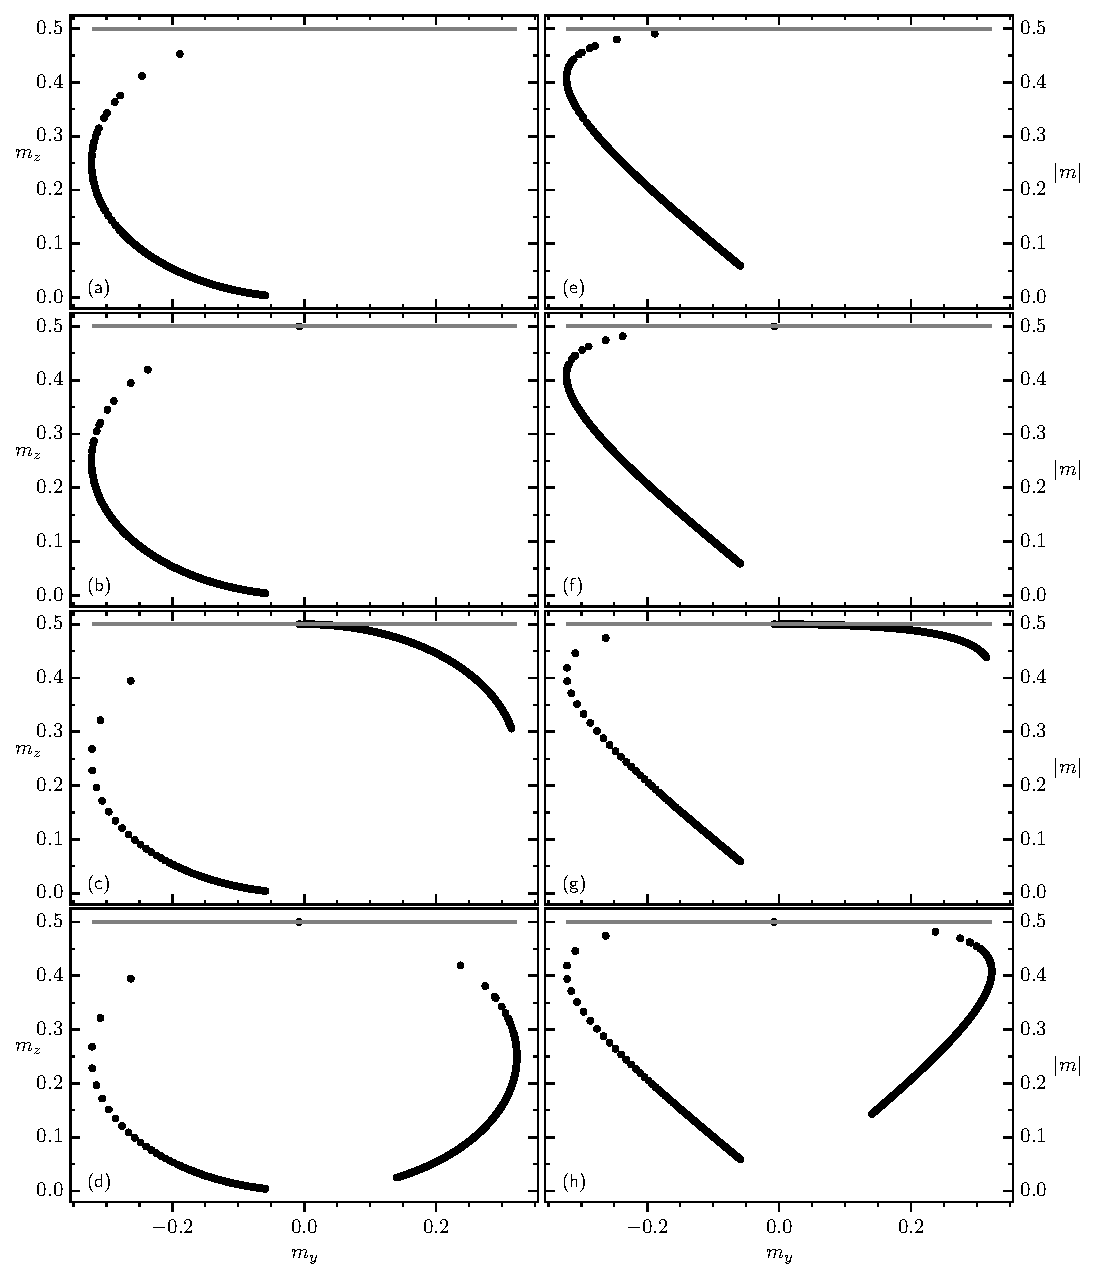
\includegraphics{pictures/fixp_boundaries.pdf}
        \caption{This graphic showes the range of $m_y$, $m_z$, $|m|$ for a parameter grid of $1.2\leq\kappa\leq24$ and $3\cdot10^{-7}\leq\omega\leq7$, $\Gamma=1$ $\gamma=0.2$. In the left column (a-d) the fixed points are shown in the $y-z$-plane, whereas in the right column (e-h) the modulus of the total angular momentum is depectid in dependence of $m_y$ for the different parameter values. The first row shows the fixed point in the parameter regime, where there is only one fixed point present. From the 2. row downwards the fixed points in the area of three stationary solutions are show in the order smallest, middle and largest $m_y$-value.}
    \end{figure}
    
    
    
    \section{Linearization eigenvalues for the unstable fixed points in the case $\delta=0$}
    \label{appendix:eig_del0}
    In this section of the appendix the eigenvalues of the linearization matrix for fixed points with middle and largest $y$-value are depicted. They show again their instability.
    \begin{figure}[H]
        \centering
        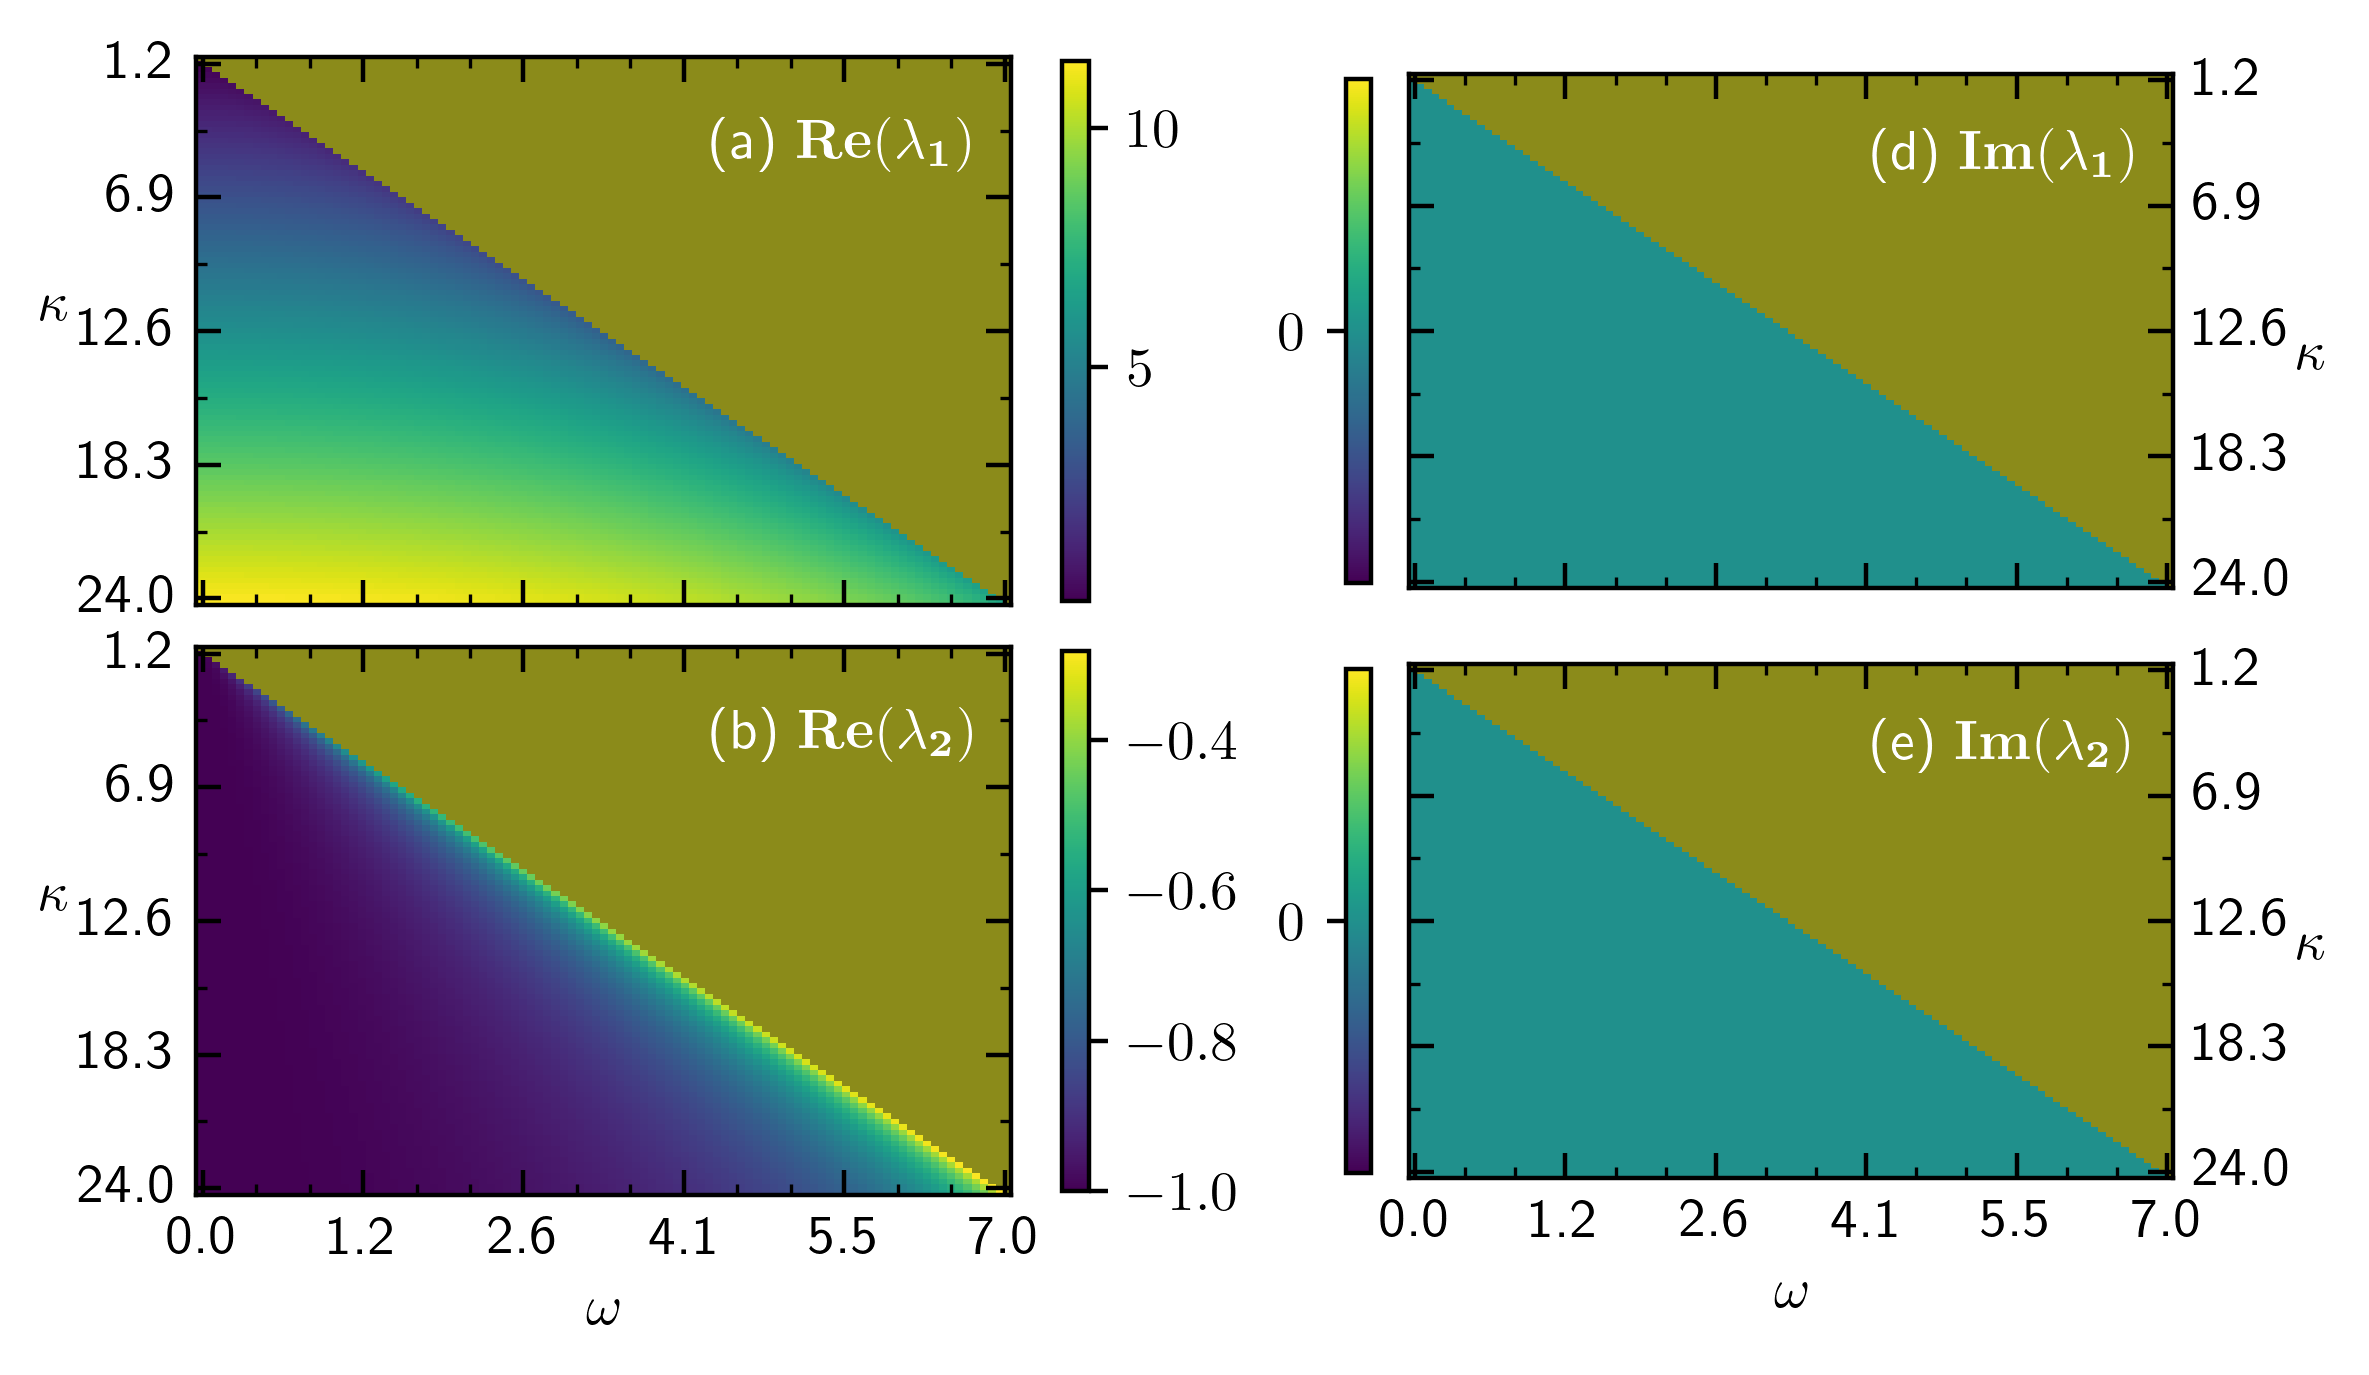
\includegraphics{pictures/lam_anal_m1.png}
        \caption{Real and imaginary part of the two of the eigenvalues of the linearization for the middle-$y$ stationary solution.
        }
    \end{figure}
    
    \begin{figure}[H]
        \centering
        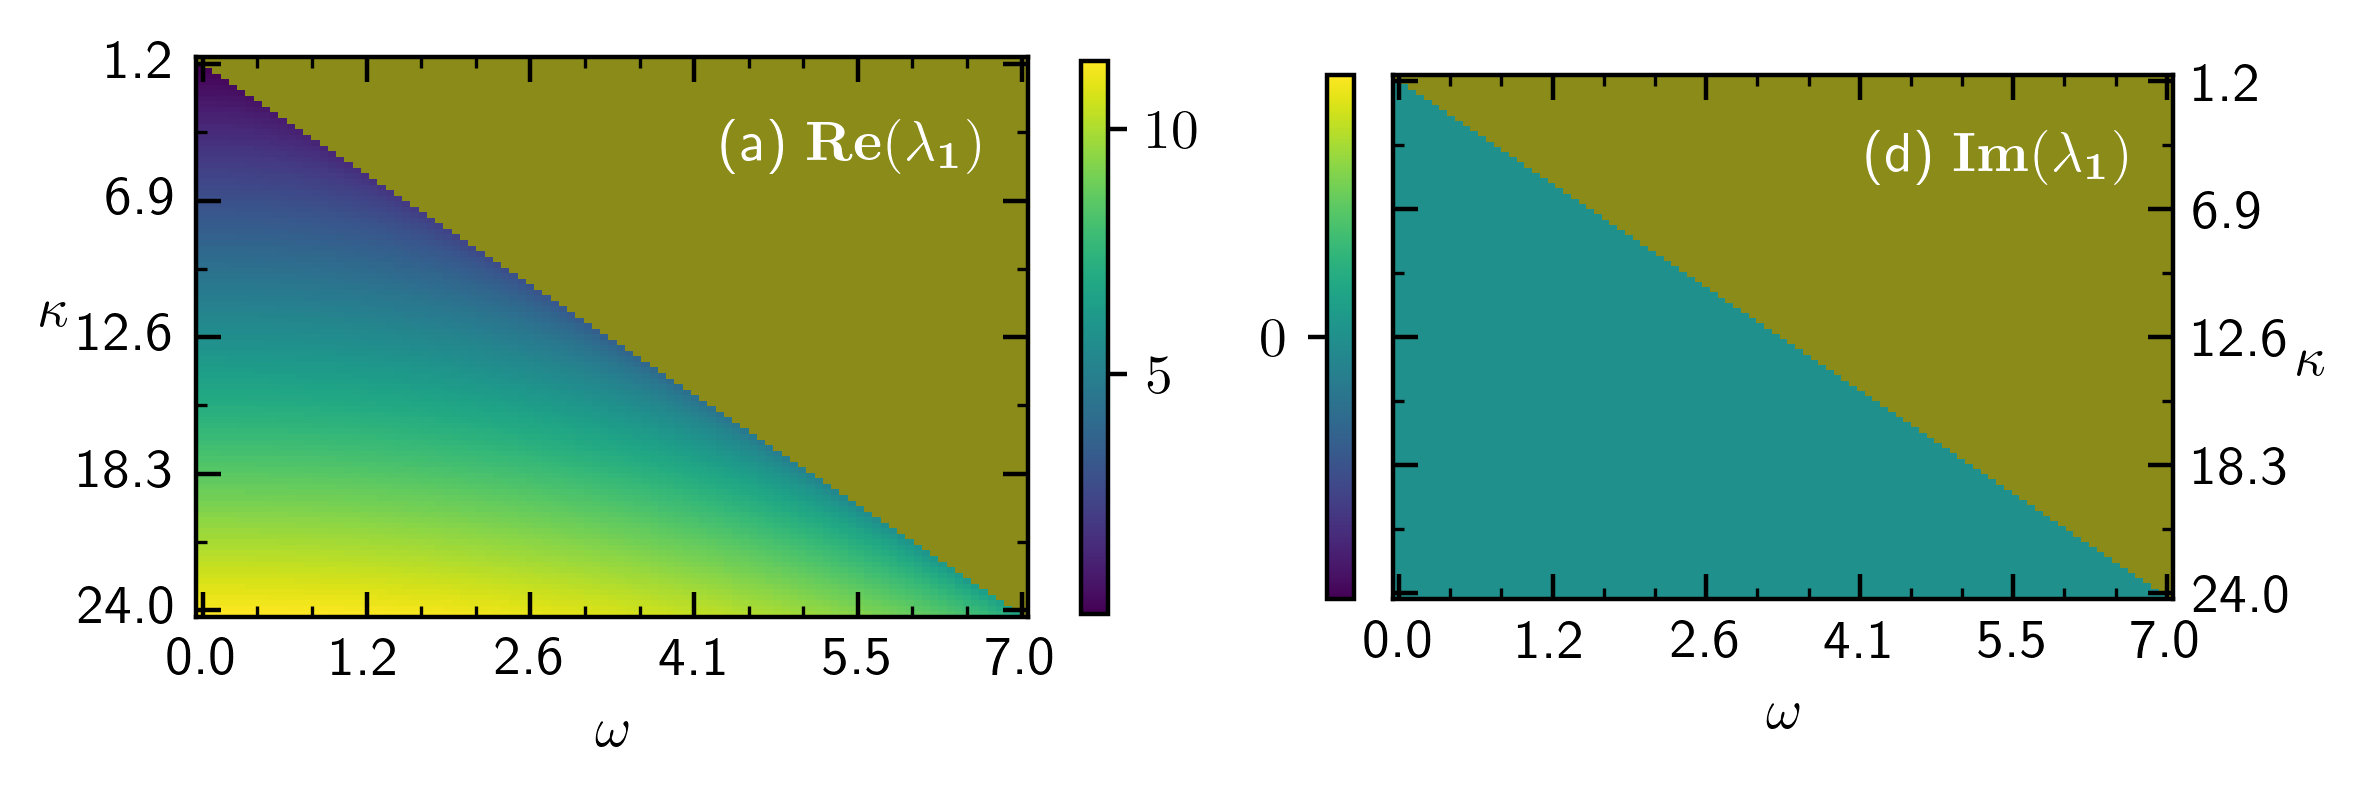
\includegraphics{pictures/lam_anal_m2.png}
        \caption{The remaining eigenvalue of the linearization for the the middle-$y$ stationary solution.
        }
    \end{figure}
    \begin{figure}[H]
        \centering
        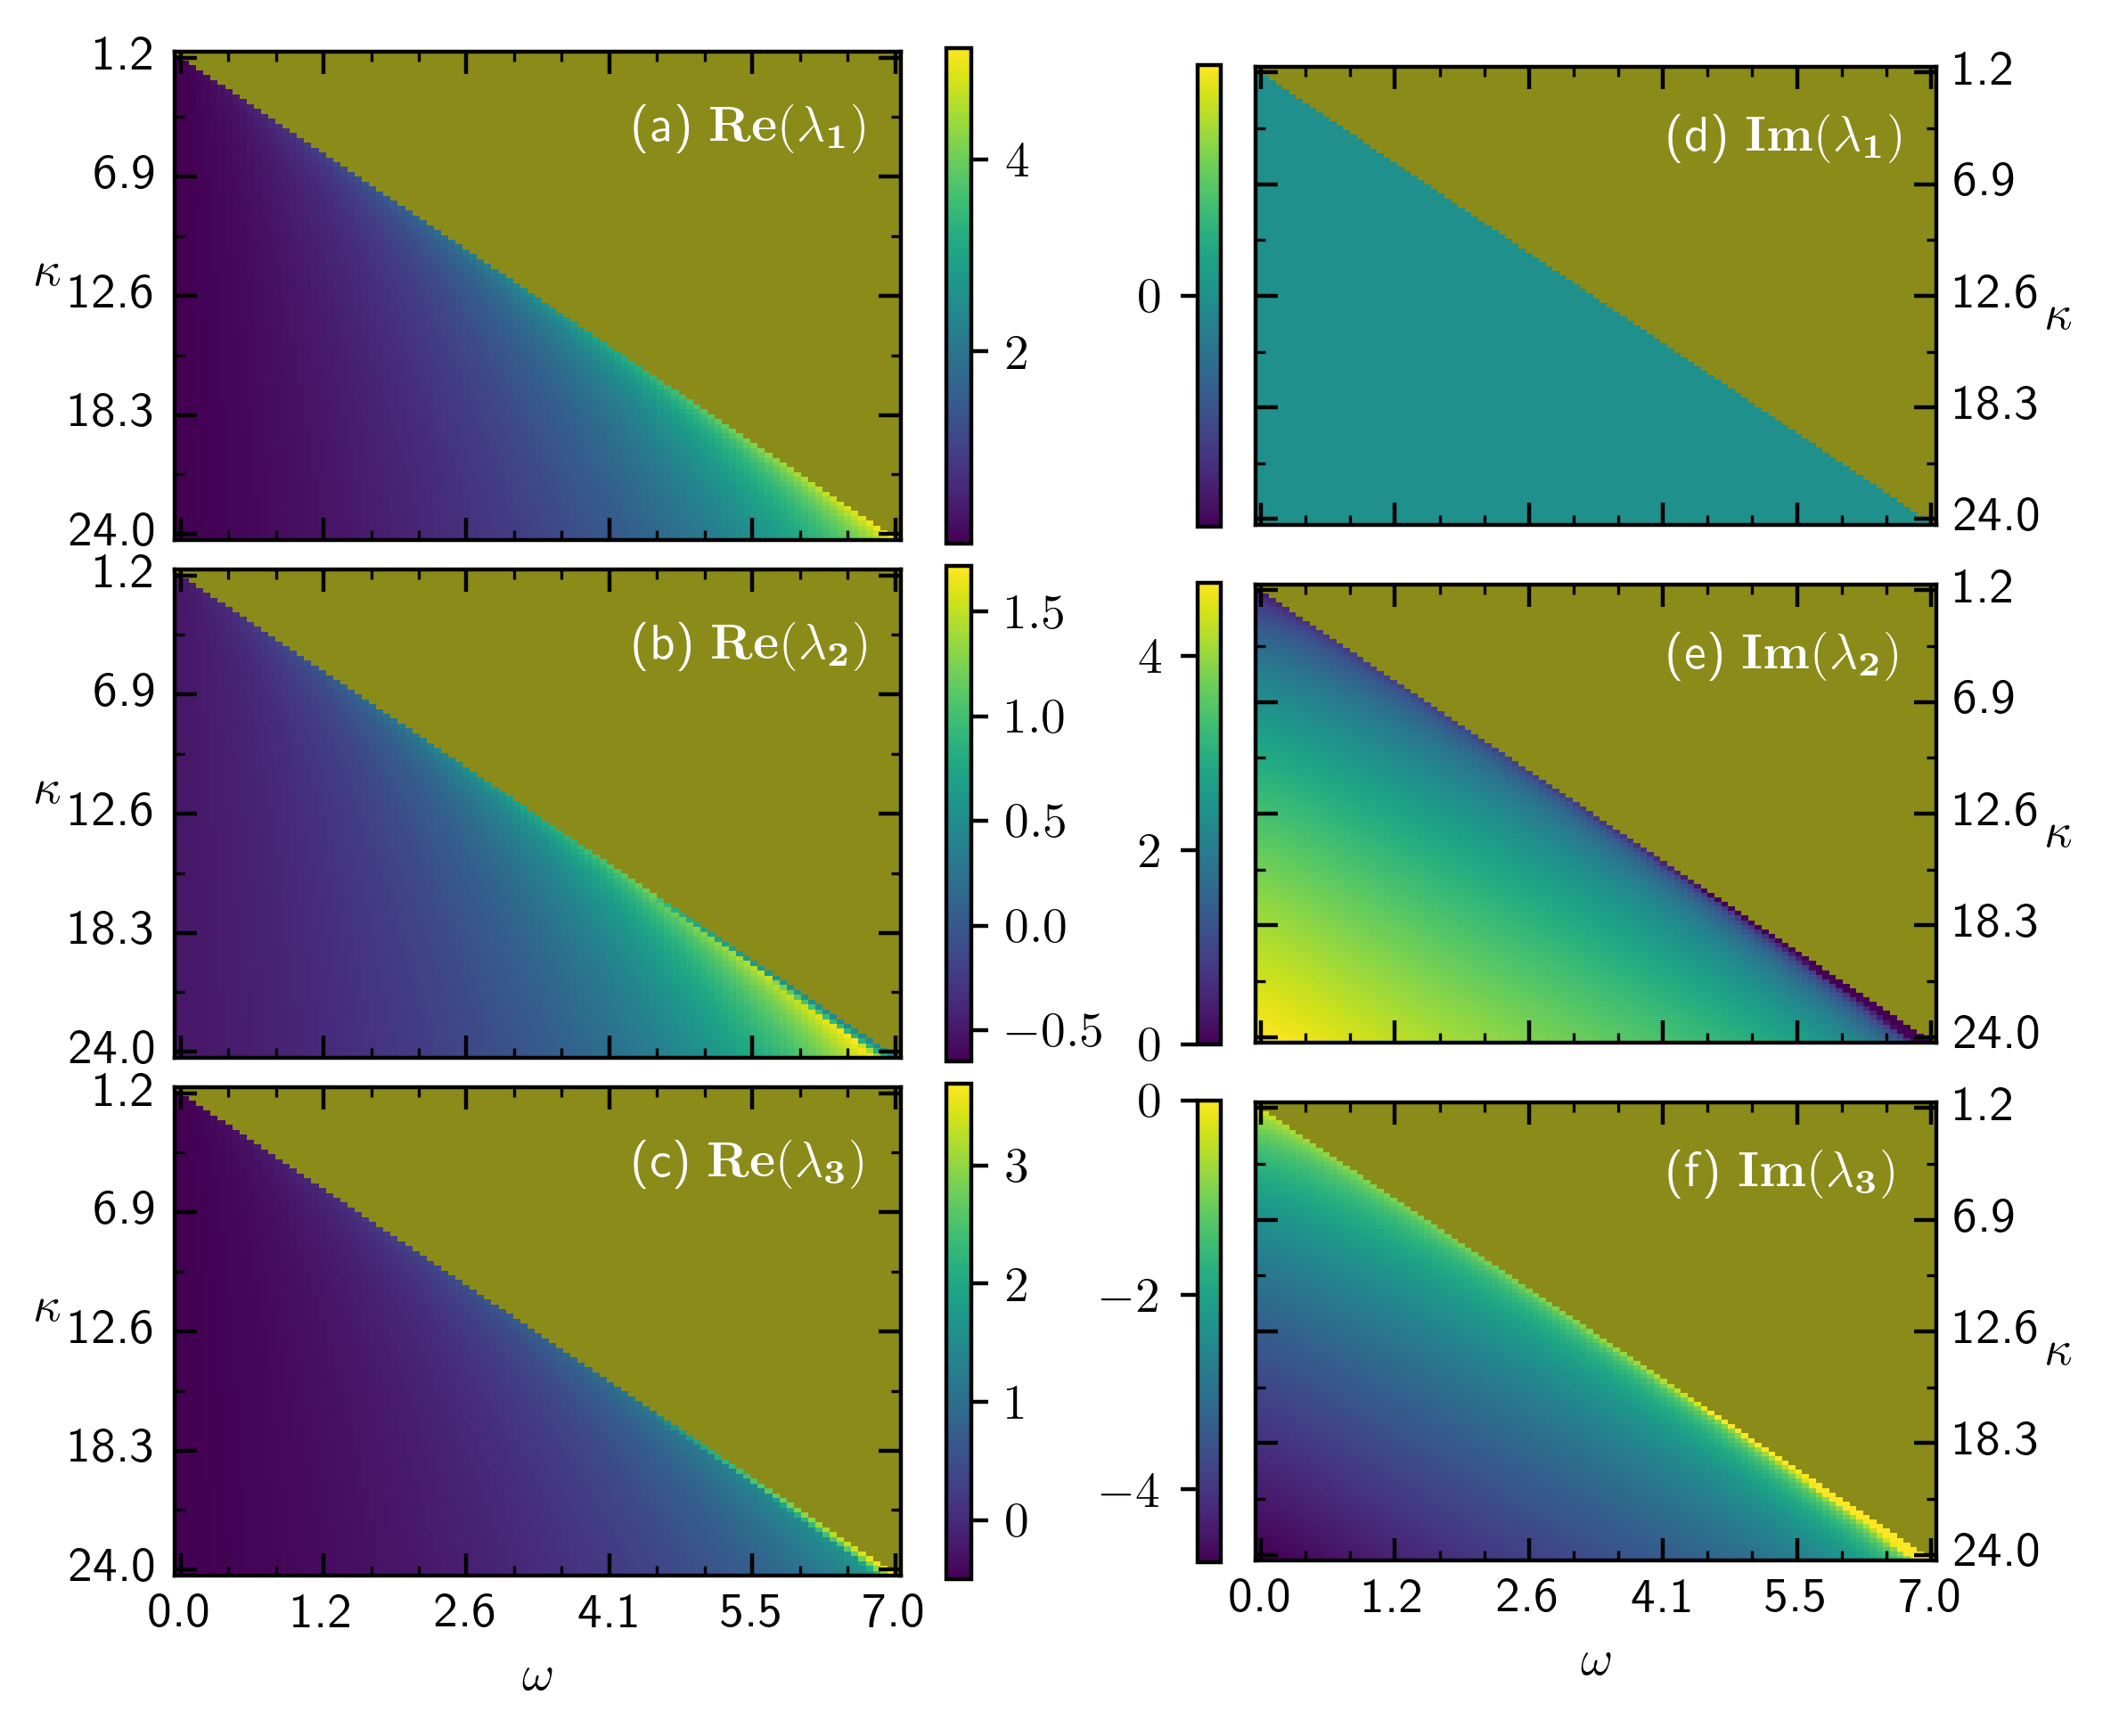
\includegraphics{pictures/lam_anal_l.png}
        \caption{Real and imaginary part of the eigenvalues from the linearization of the equations of motion are shown for the largest $y$-value fixed point.
        }
    \end{figure}
    
    \chapter{Appendix for the model with detuning}
    \section{Exemplary trajectories}
    \label{appendix:expl_traj}
    This paragraph shows a few exemplary long-time states of the system for the area where the transition of $m_x$-values is accompanied by multistability. Therefore I reconsider the outstanding regions in \figref{fig:fixedpoint_colormap} of \secref{sec:detuned_analysis}. I divide those regions into 9 parts and select randomly a parameter configuration out of those areas. For a few random initial conditions I depict the resulting long-time states.
    \begin{figure}[H]
        \centering
        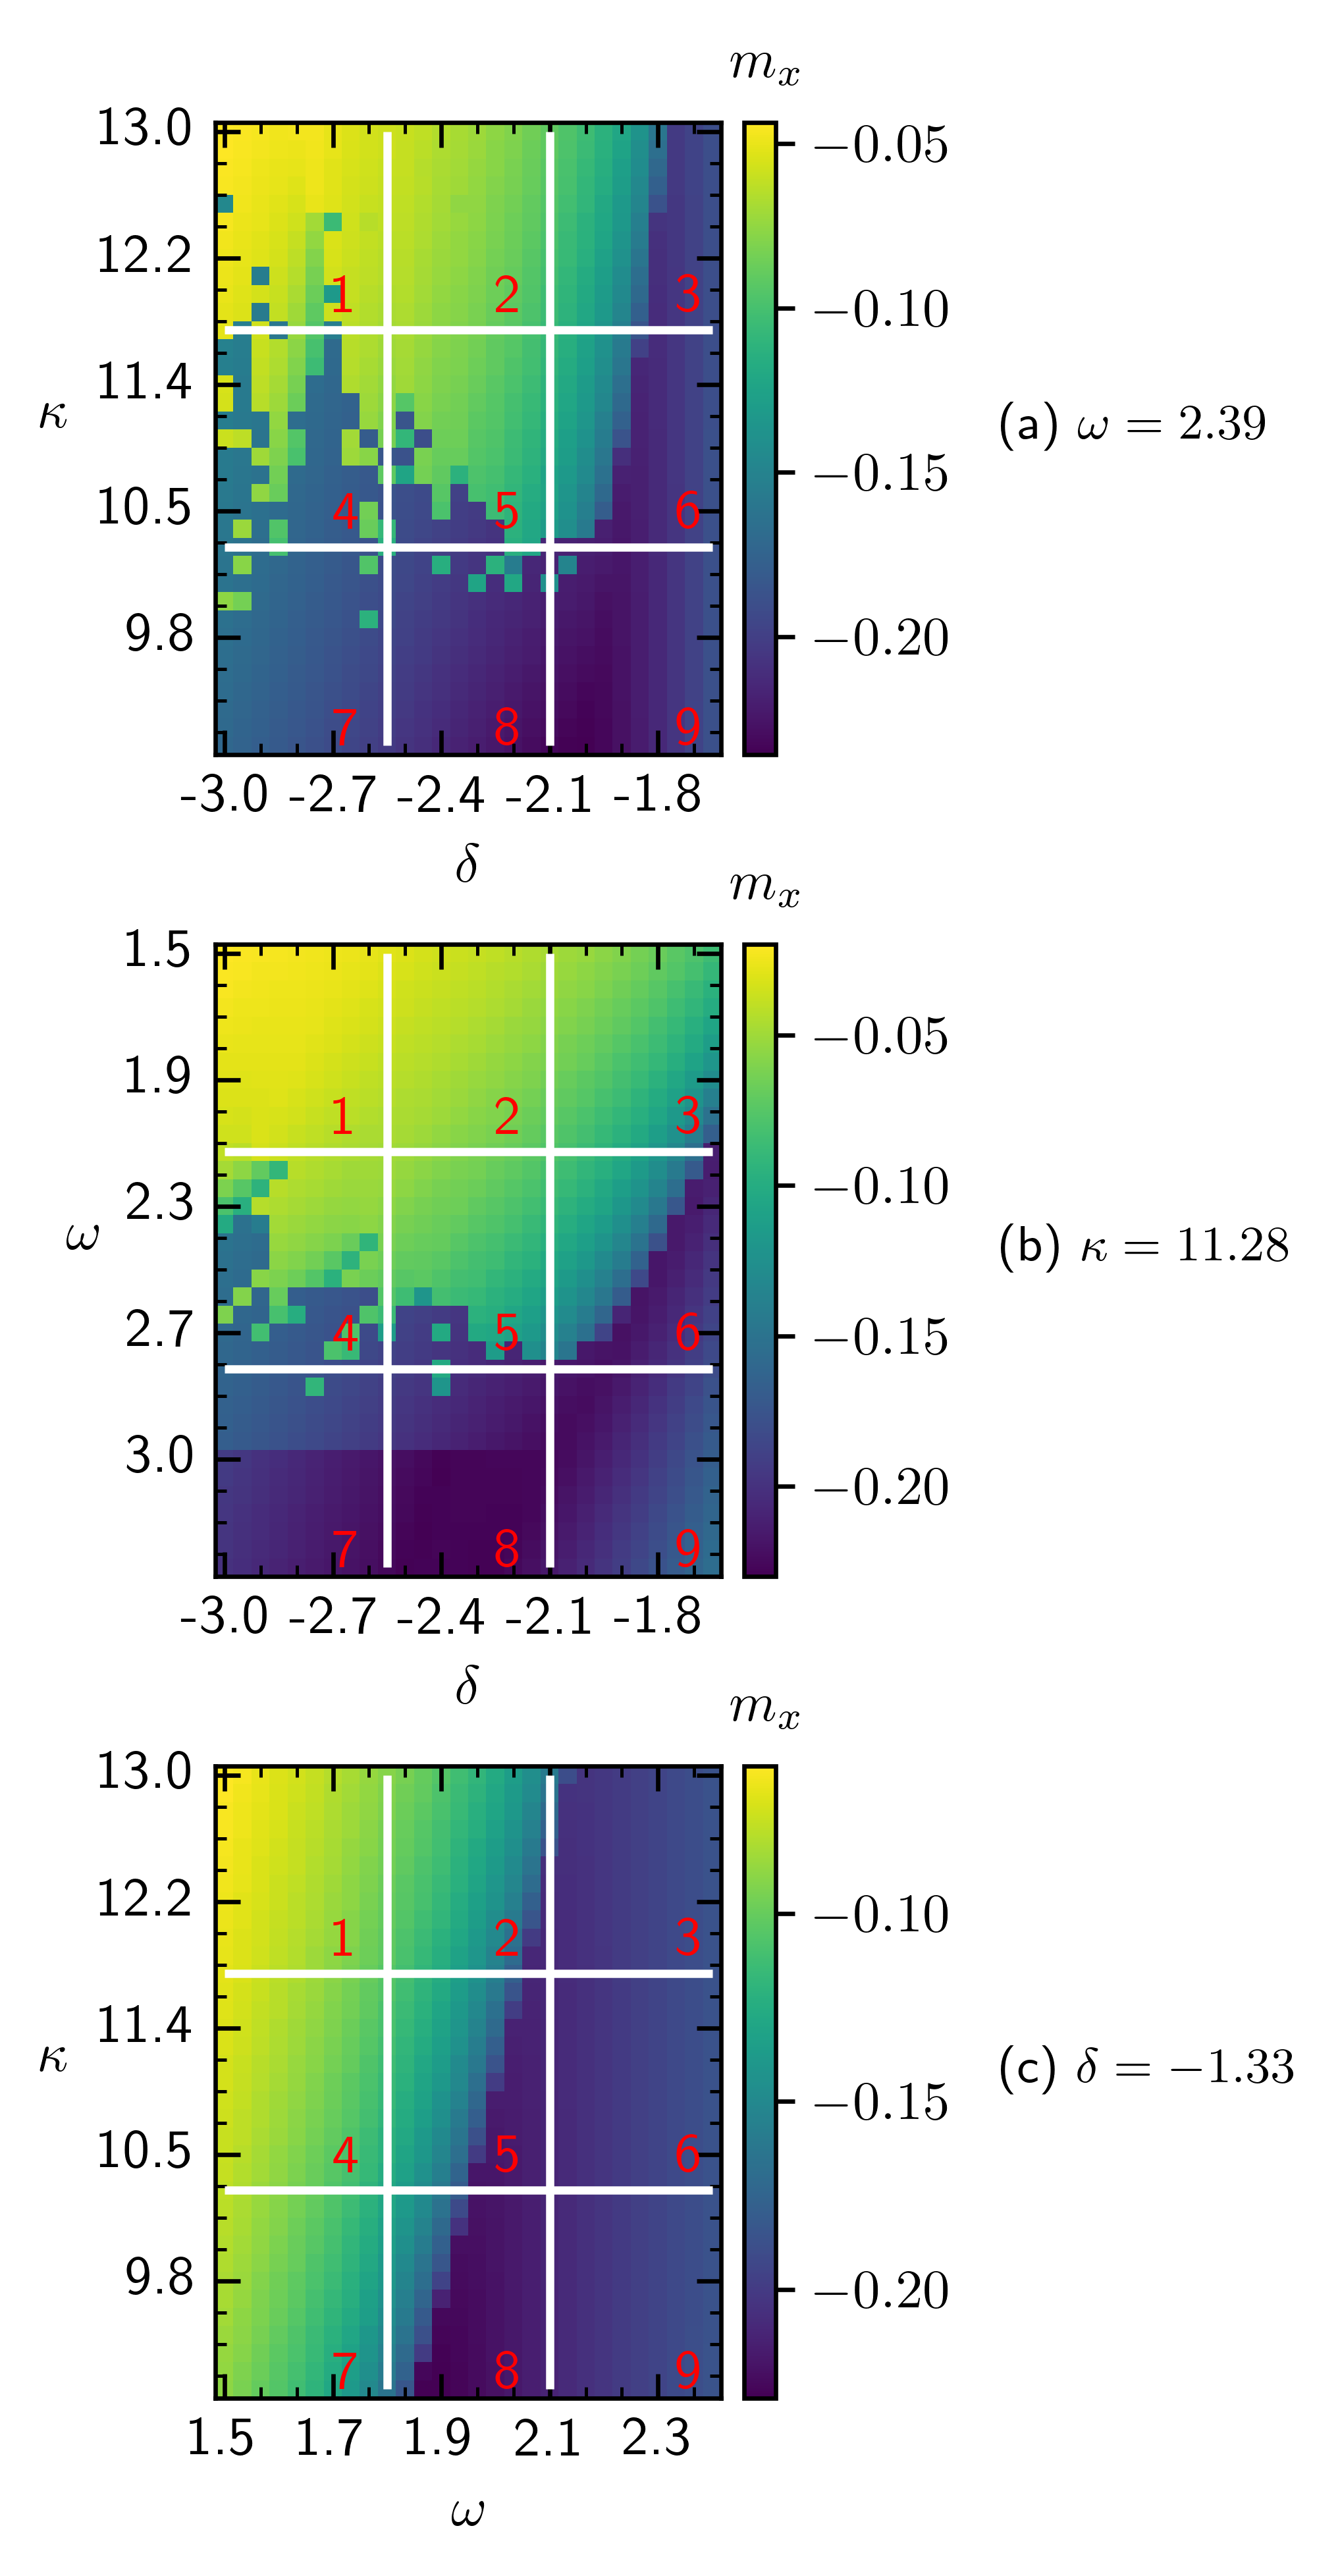
\includegraphics{pictures/combined_spec_sec.png}
        \caption{The division of the outstanding areas of \figref{fig:fixedpoint_colormap}.}
    \end{figure}
    
    \begin{figure}[H]
        \centering
        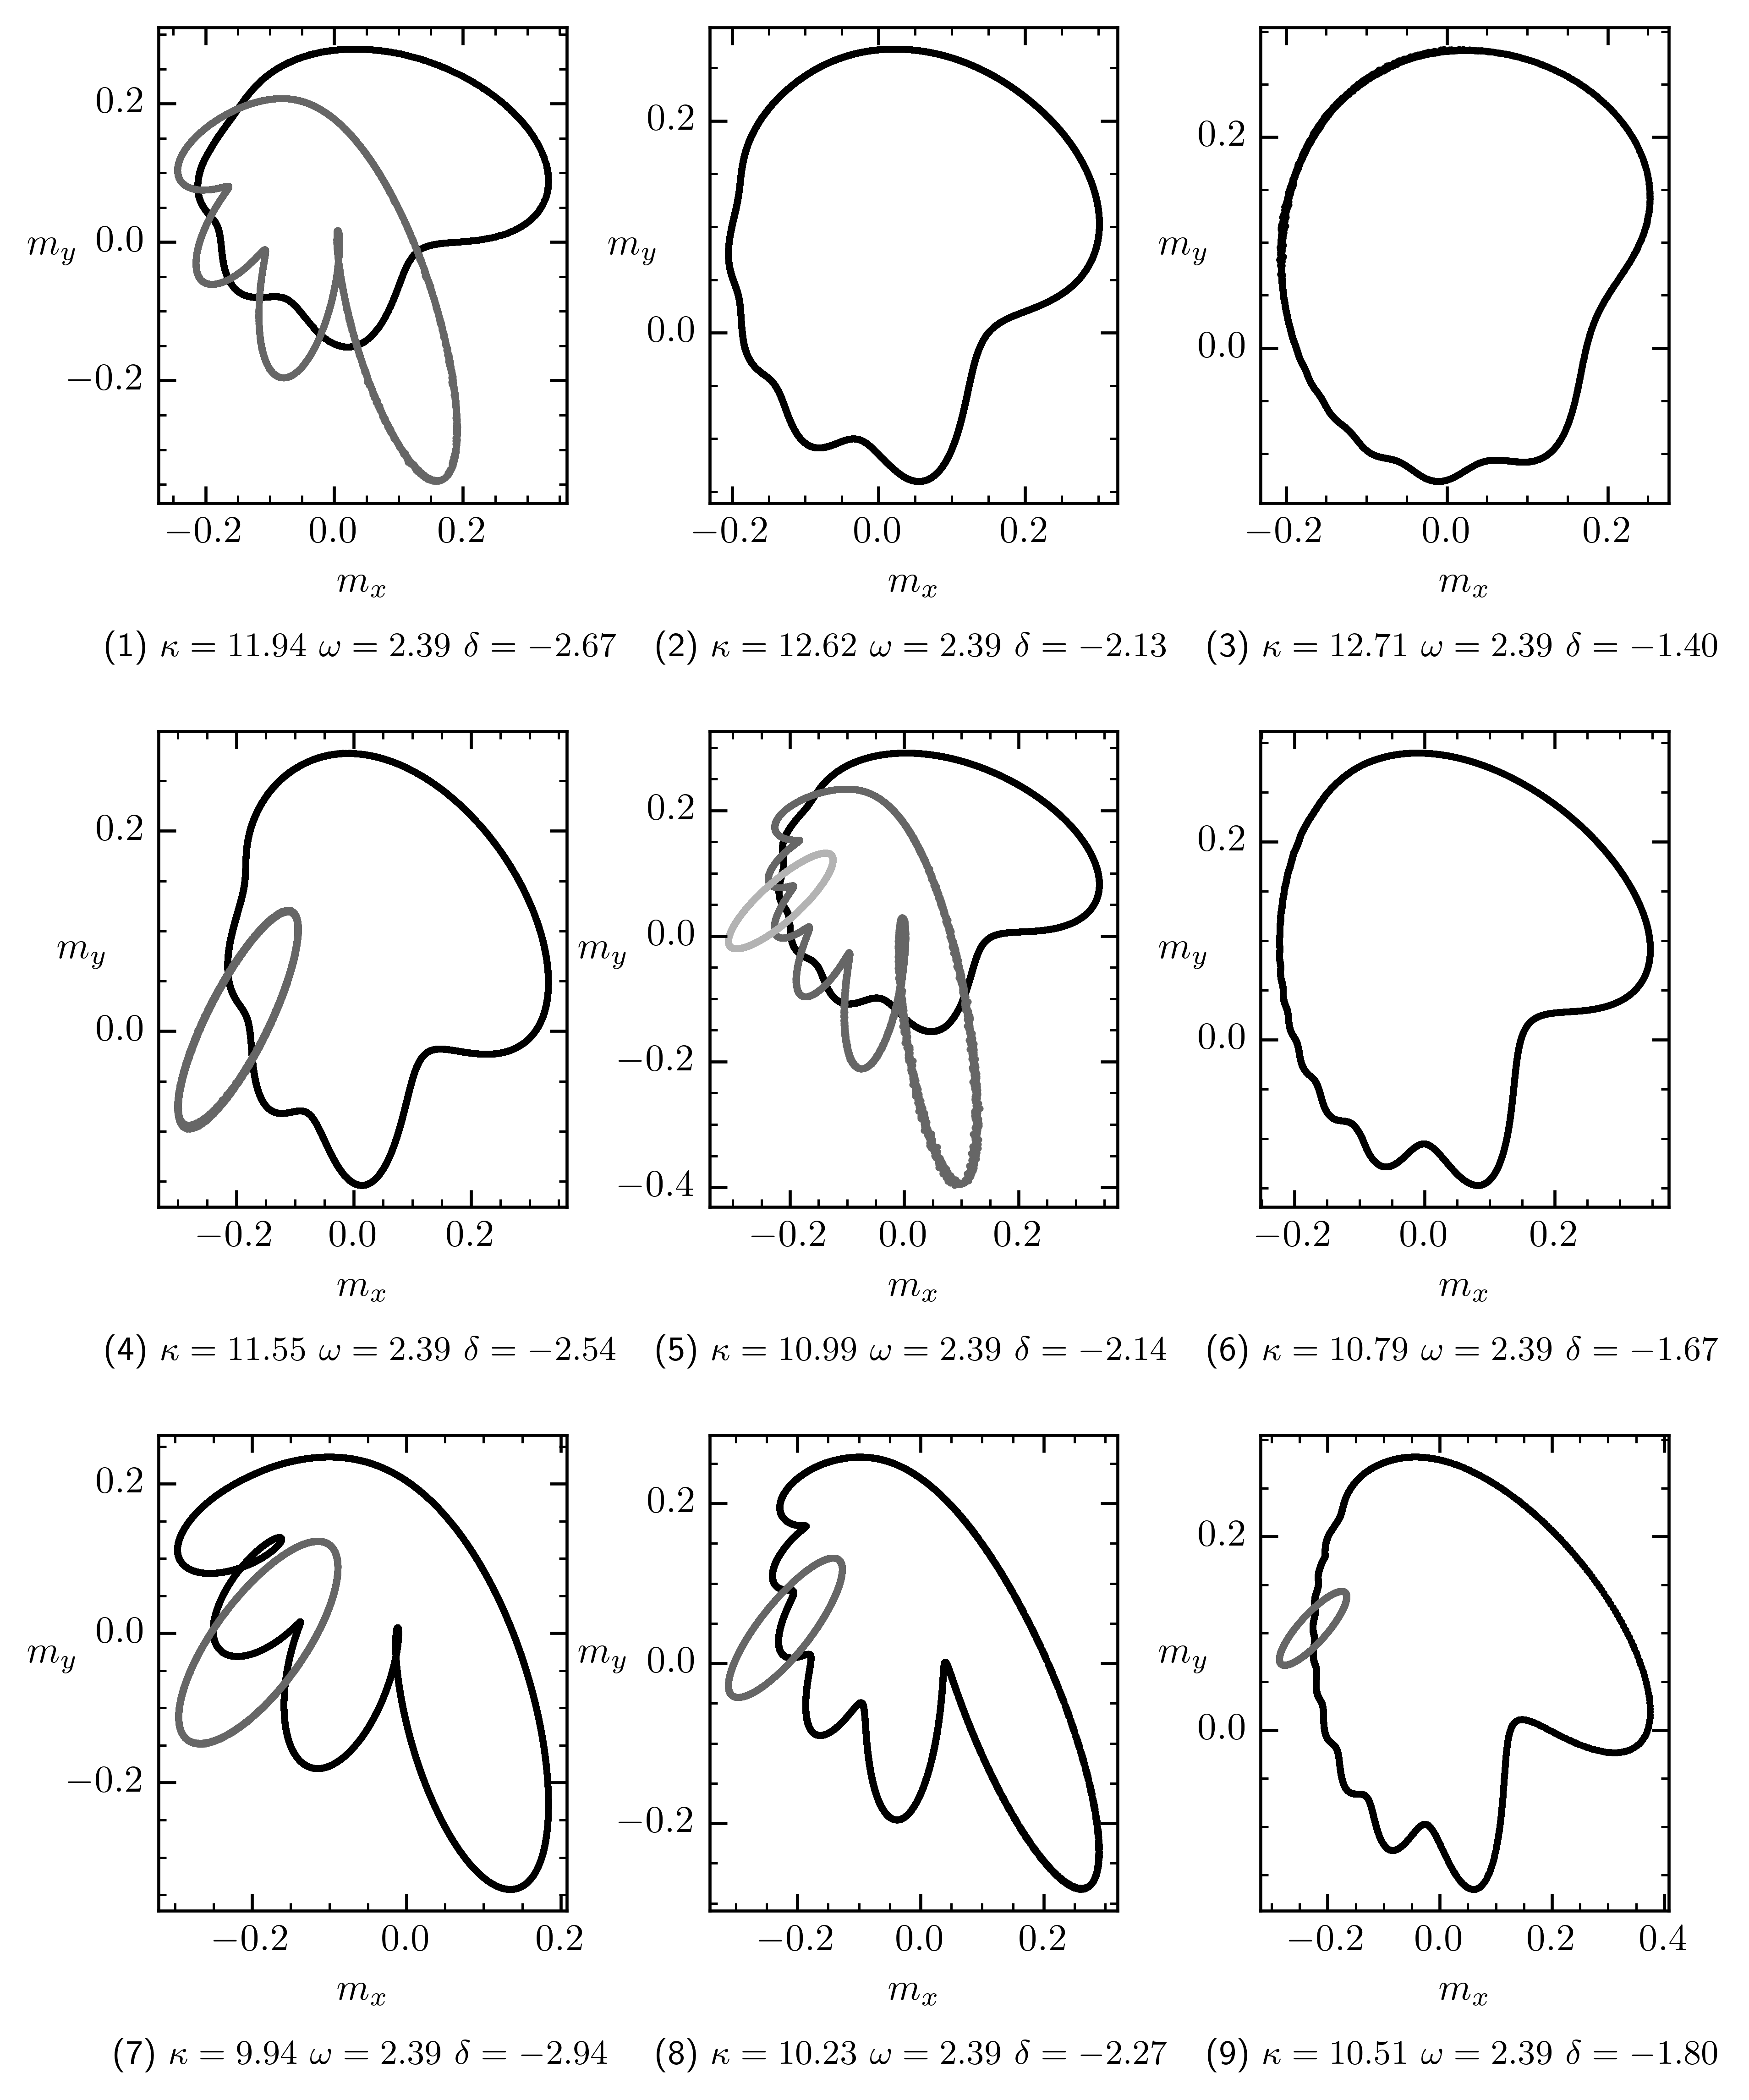
\includegraphics{pictures/lc_traj_wcut3.png}
        \caption{For $\omega=2.389$ possible long time states are shown for random values from the parameter grid. Where stationary points exist, I also drew the transition from the starting points to the stationary point.}
    \end{figure}
    
    \begin{figure}[H]
        \hspace*{-1cm}
        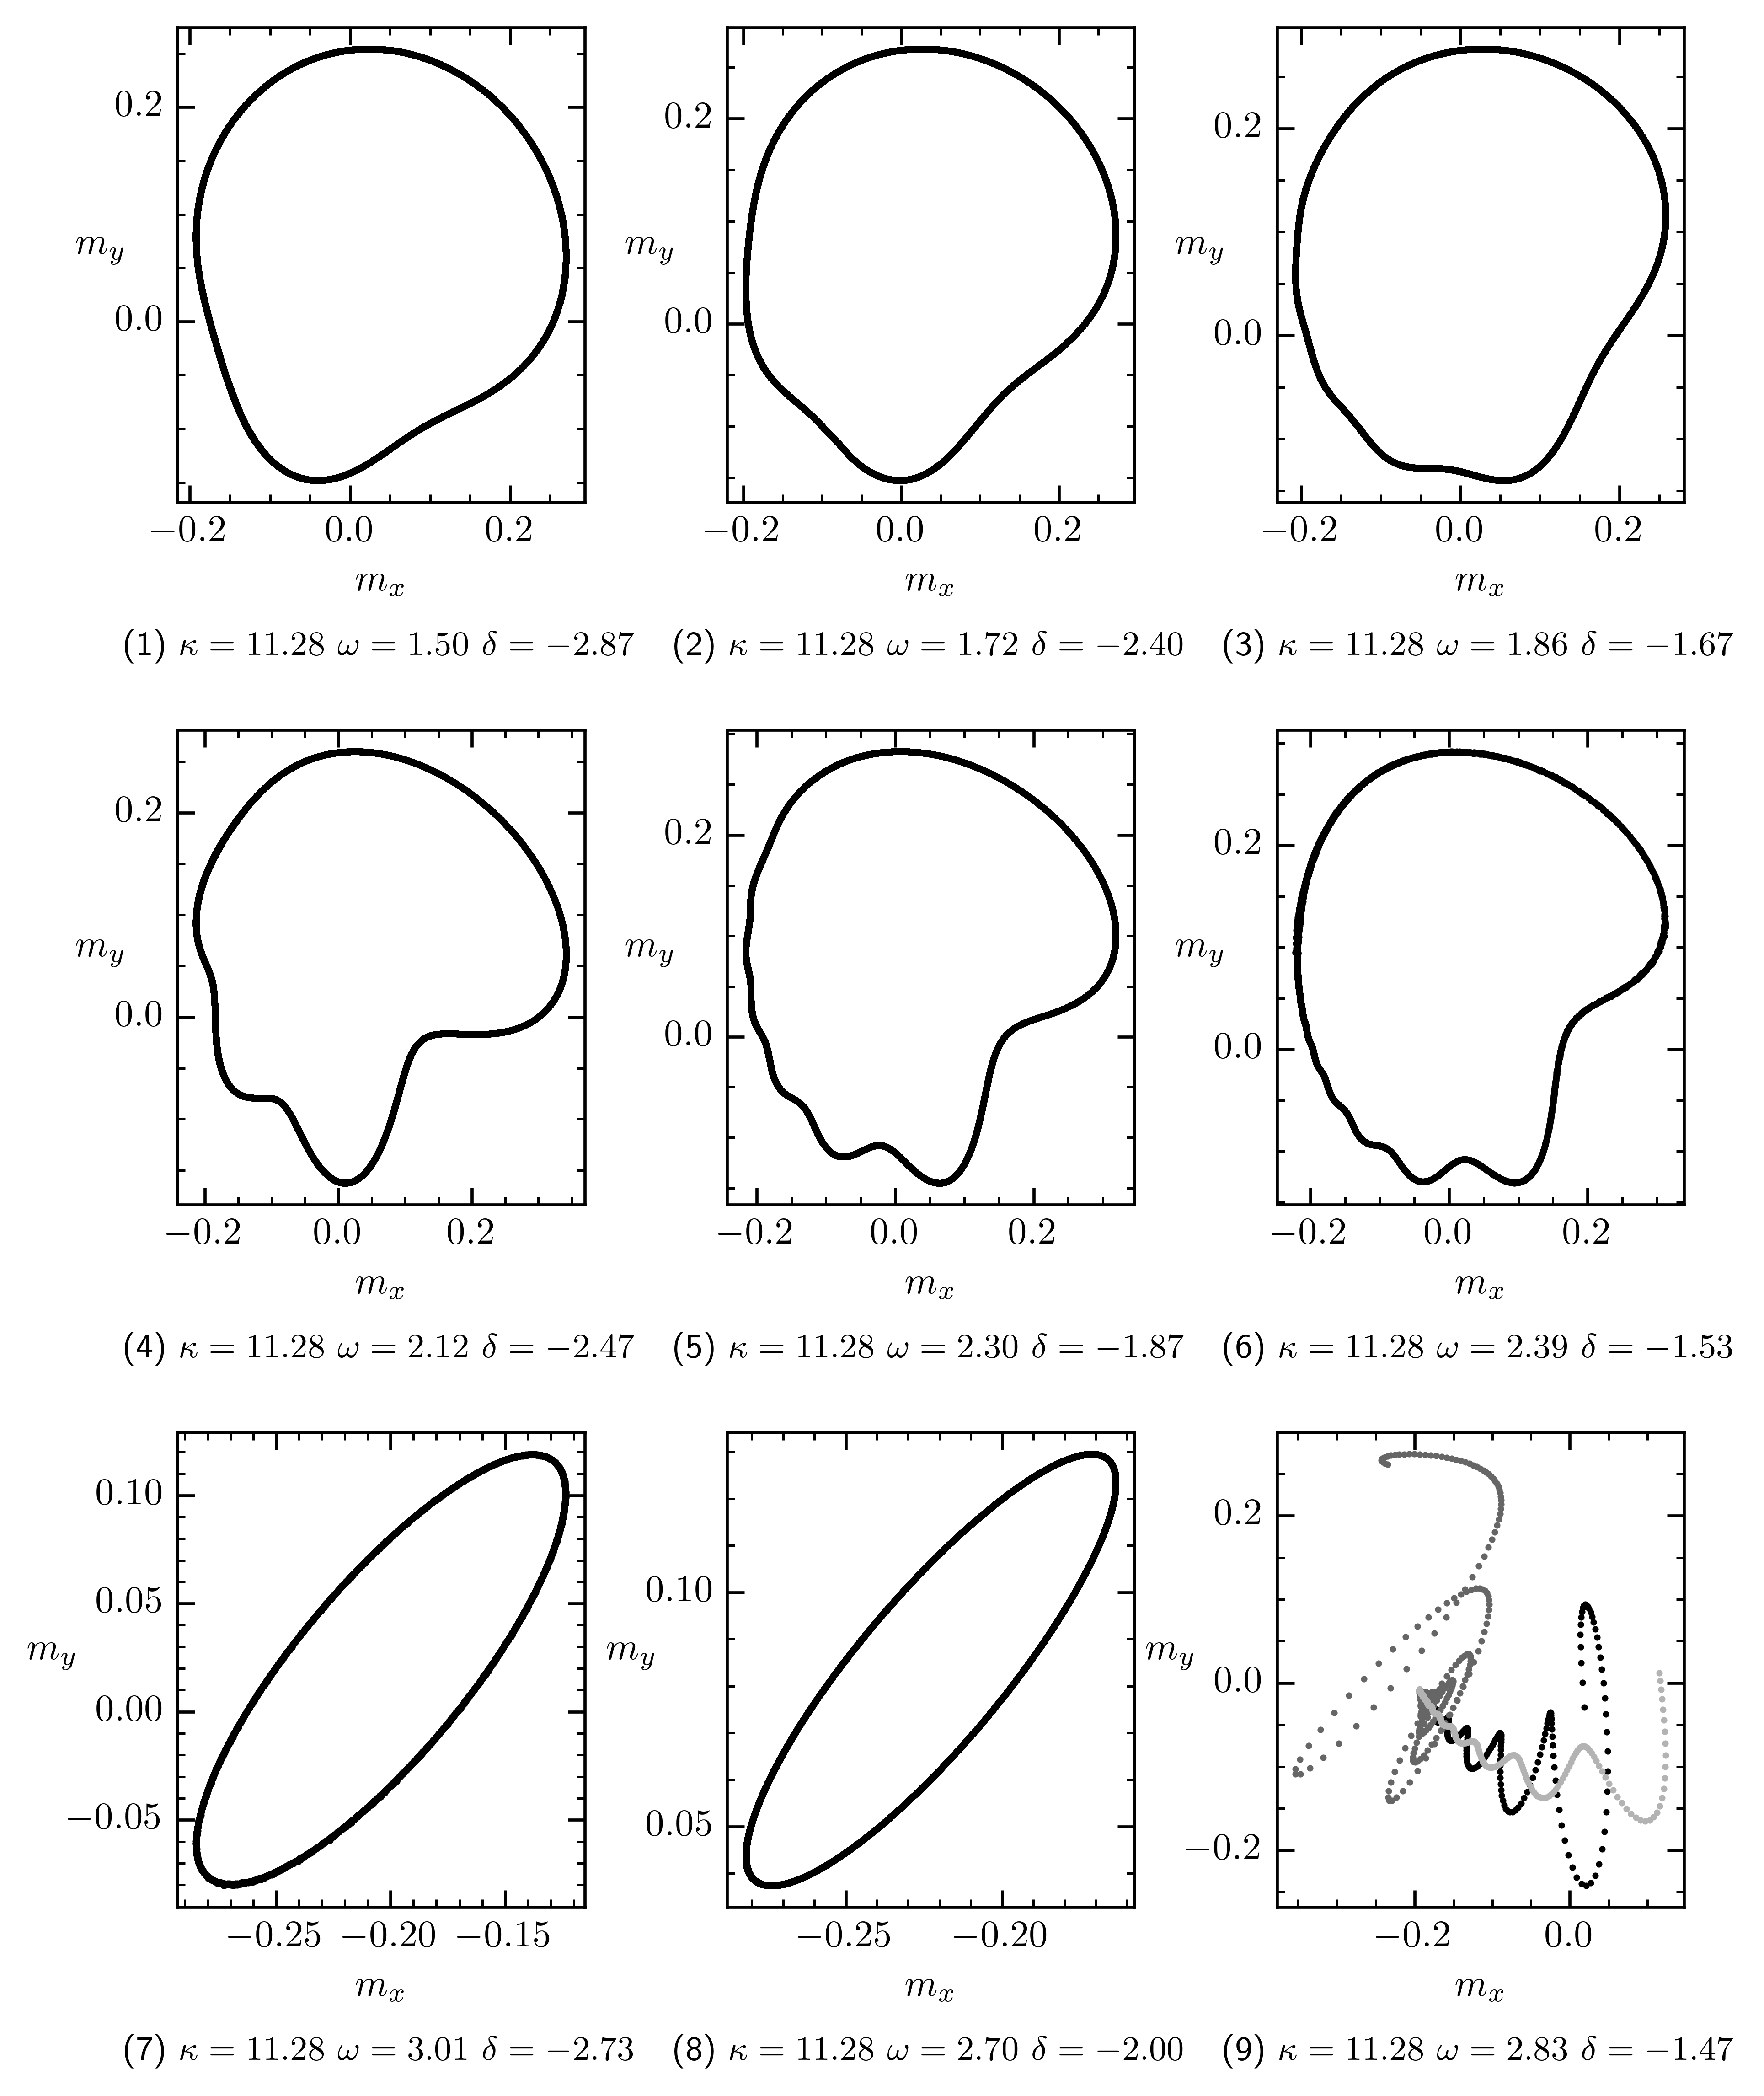
\includegraphics{pictures/lc_traj_kcut2.png}
        \caption{For $\kappa=11.28$ possible long time states are shown for random values from the parameter grid. Where stationary points exist, I also drew the transition from the starting points to the stationary point.}
    \end{figure}
    
    \begin{figure}[H]
        \centering
        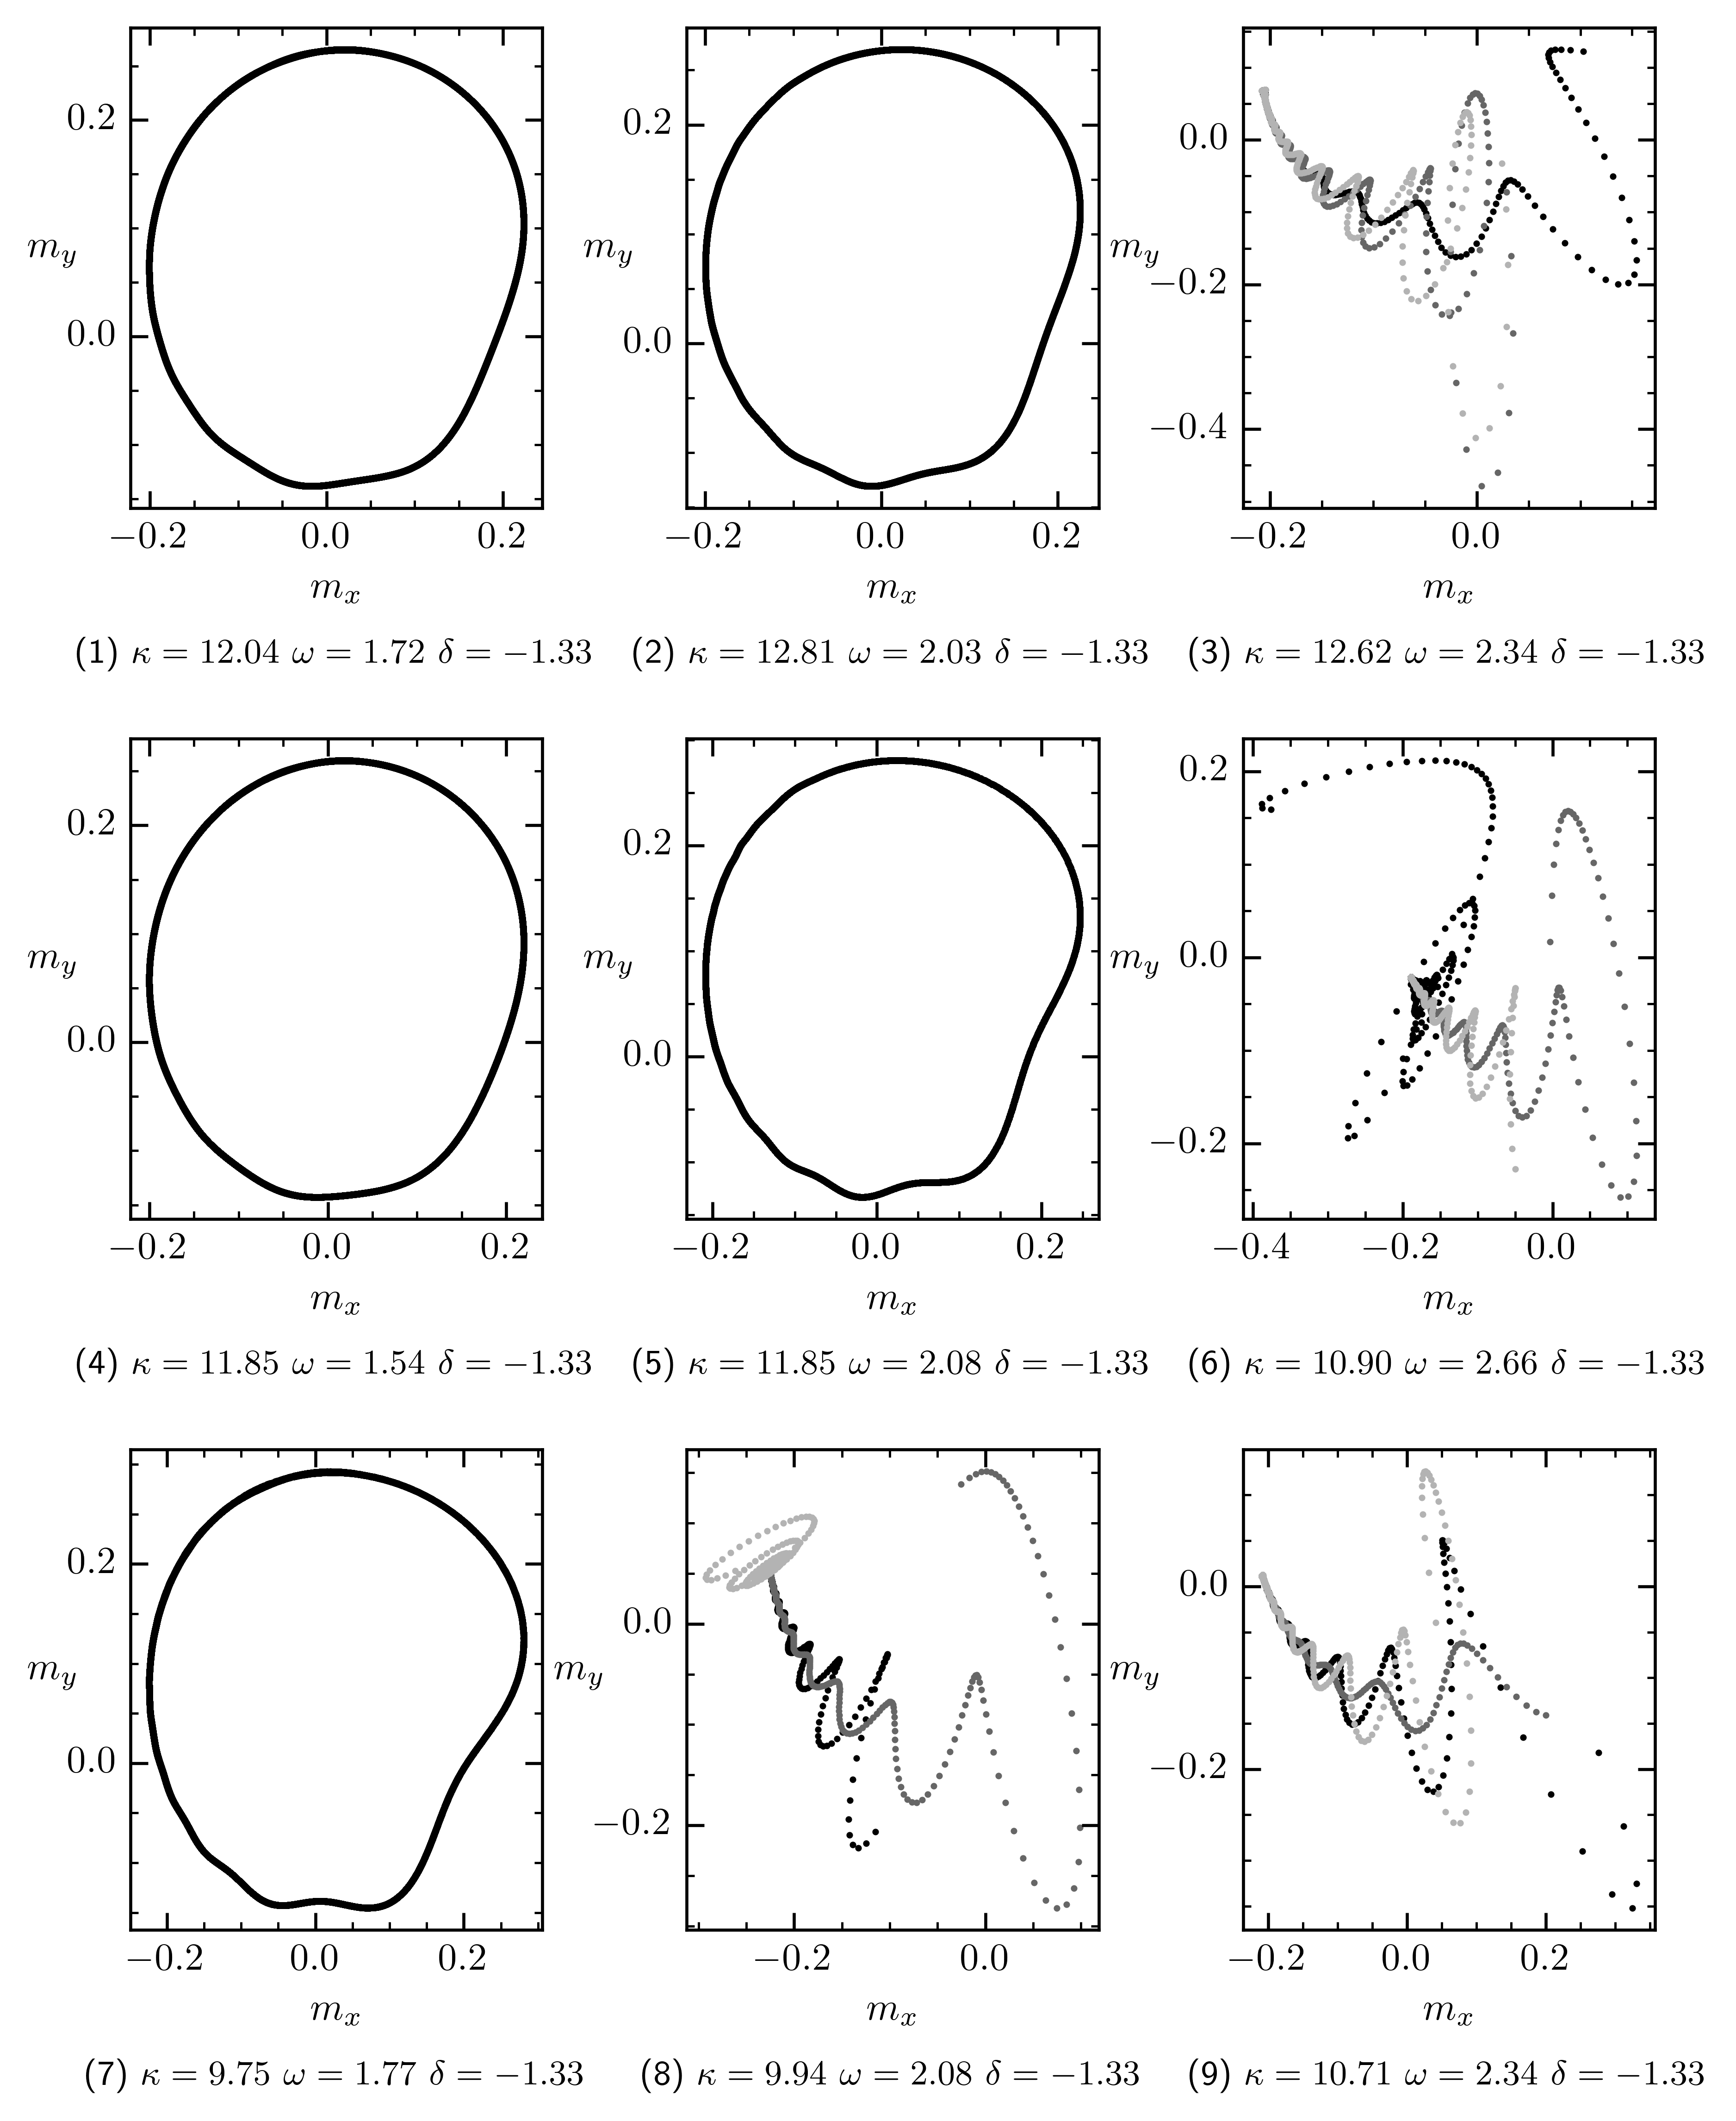
\includegraphics{pictures/lc_traj_dcut2.png}
        \caption{For $\delta=-1.33$ possible long time states are shown for random values from the parameter grid. Where stationary points exist, I also drew the transition from the starting points to the stationary point.}
    \end{figure}\newpage

    \section{Long-time states for varying dephasing strength}\label{app:gamma_analysis}
    An examination of the long-time states for different $\gamma$-values, which has been omitted in the main text, is briefly carried out at this point. For this purpose I again plot the stationary points as well as the average over a period of a limit cycle for different parameter values.
    \begin{figure}[H]
        \centering
        \caption{fixed points and averaged limit cycles over their period. In (a) $\gamma$ and $\delta$ are varied, while the other parameter a kept fixed. In (b) the cut with differing $\omega$ and $\delta$ is repeated for a different $\kappa$ and more importantly a different $\gamma$ value. $\Gamma=1$ as always. The white dashed line separates the region of limit cycles from that where stationary points exist. In both plots the area above the white line is the time crystal phase.}
        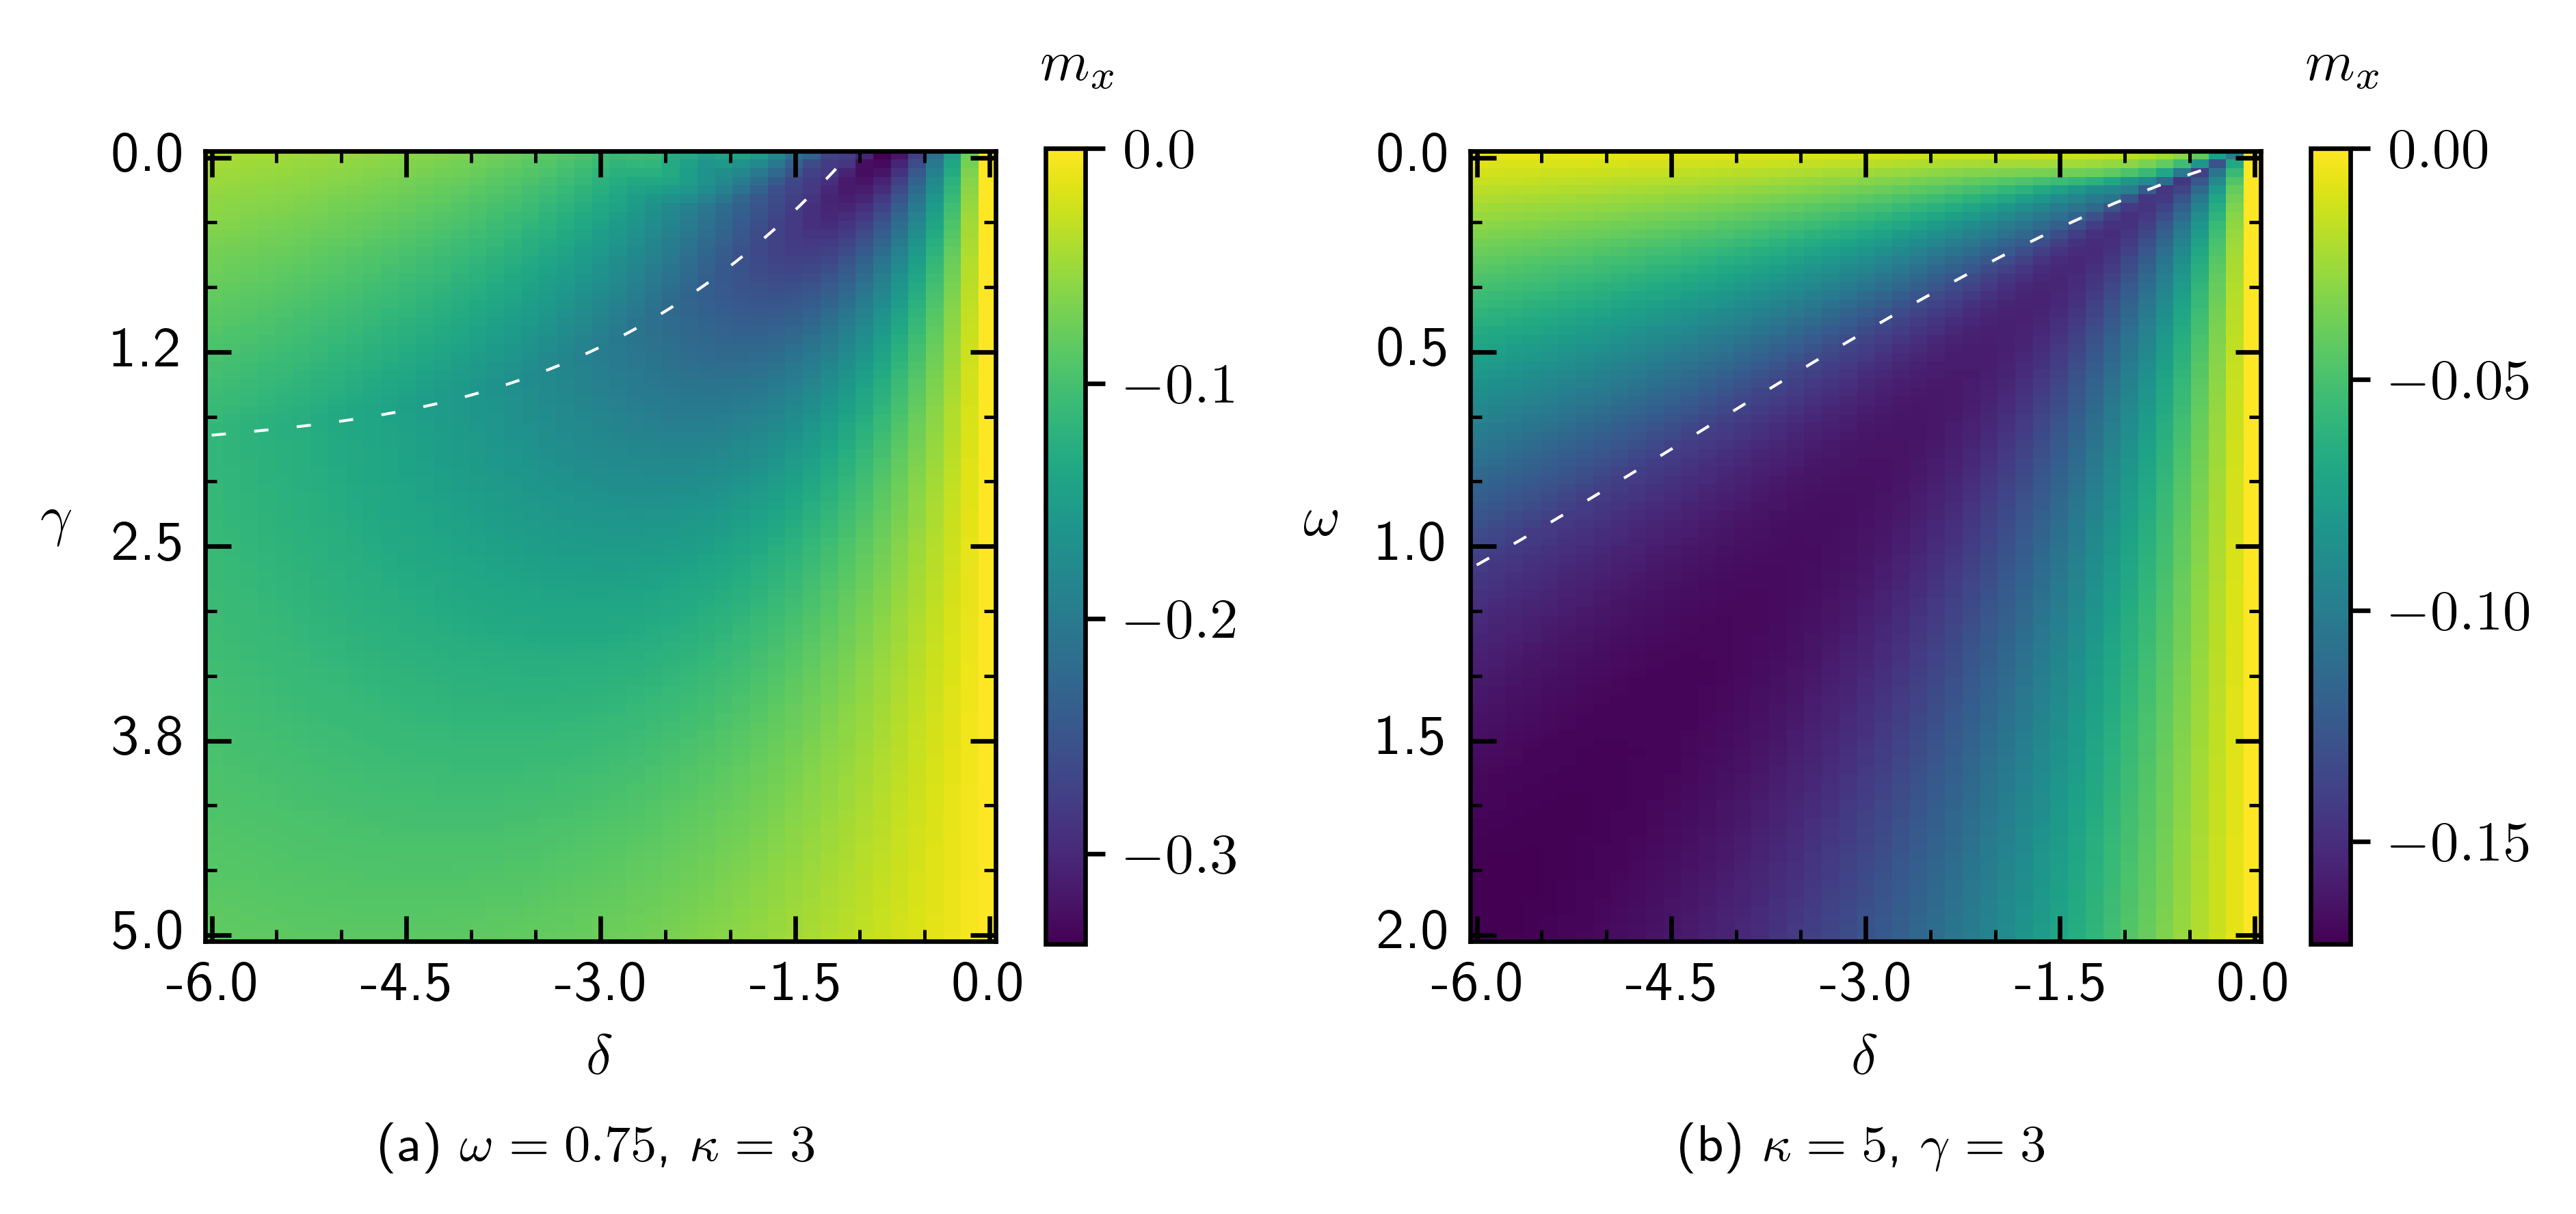
\includegraphics{pictures/limit_cycle_mean_gw.png}
        \label{fig:gamma_longtime}
    \end{figure}
    A several interesting observations can be made. Starting with \figref{fig:gamma_longtime}(b) one can see that the phase separation line has qualitatively the same shape as for $\gamma=0.2$. It again follows the property of synchronization effects that the larger the detuning between the considered systems is the larger the coupling between them has to be in order to see synchronization. I can also inform the reader that the parameter set that has been chosen in \figref{fig:gamma_longtime}  exhibits no multistability. For all configuration only one limit cycle or one stationary solution exists. \\
    What can be additionally observed is that the long-time states show a valley of small $m_x$ values, that lies near the phase separation line but does not coincide with it. \\\\
    Turning to \figref{fig:gamma_longtime}(a) one finds that the time crystal phase is stable for a wide range of dephasing strength for certain parameter constellations. What is also intriguing is that the higher $\gamma$ is the larger, in absolute value, the detuning has to be in order to observe a time crystal phase. The form of the phase separation line also suggests that there might be a maximal value of dephasing such that above that value no limit cycles can arise. But this definitively has to be yet verified, what could be an interesting subject of future analysis.




% \end{appendices}
% % \clearpage

% {
% 	\thispagestyle{plain}
% 	\chapter*{}
% 	\section*{Acknowledgements}
% 	First and foremost, I thank my two supervisors, Prof. Dr. Igor Lesanovsky and Dr. Federico Carollo. Your guidance, support, and mentorship have been invaluable throughout my master thesis and the related publication. After each of our discussions, I felt old questions answered and new ones raised.

% 	Of course, my gratitude also belongs to Prof. Dr. Daniel Braun, who appraised this thesis despite his current research semester.

% 	Also, I wish to extend my thanks to Priv.-Doz. Dr. Beatriz Olmos Sanchez, Chris Nill and Tom von Scheven. Your advices, encouragement and the professional exchange in each and every project during the last year provided me with a new perspective and have helped me approach problems from different angles. 

% 	Finally, I want to thank Moritz Eissler for proofreading this thesis and contributing valuable suggestions for its presentation. 
	
% 	\clearpage
	
% 	\thispagestyle{plain}
% 	\section*{Contact Information}
% 	Marcel Cech\\
% 	Institut für Theoretische Physik\\
% 	Auf der Morgenstelle 14\\
% 	Universität Tübingen\\
% 	72076 Tübingen\\
% 	Marcel.Cech@student.uni-tuebingen.de


% }

\end{document}
